% Options for packages loaded elsewhere
\PassOptionsToPackage{unicode}{hyperref}
\PassOptionsToPackage{hyphens}{url}
\PassOptionsToPackage{dvipsnames,svgnames,x11names}{xcolor}
\documentclass[
  11pt,
  oneside]{book}
\usepackage{xcolor}
\usepackage[margin=1in]{geometry}
\usepackage{amsmath,amssymb}
\setcounter{secnumdepth}{-\maxdimen} % remove section numbering
\usepackage{iftex}
\ifPDFTeX
  \usepackage[T1]{fontenc}
  \usepackage[utf8]{inputenc}
  \usepackage{textcomp} % provide euro and other symbols
\else % if luatex or xetex
  \usepackage{unicode-math} % this also loads fontspec
  \defaultfontfeatures{Scale=MatchLowercase}
  \defaultfontfeatures[\rmfamily]{Ligatures=TeX,Scale=1}
\fi
\usepackage{lmodern}
\ifPDFTeX\else
  % xetex/luatex font selection
  \setmainfont[]{Latin Modern Roman}
  \setsansfont[]{Latin Modern Sans}
  \setmonofont[]{Latin Modern Mono}
  \setmathfont[]{Latin Modern Math}
\fi
% Use upquote if available, for straight quotes in verbatim environments
\IfFileExists{upquote.sty}{\usepackage{upquote}}{}
\IfFileExists{microtype.sty}{% use microtype if available
  \usepackage[]{microtype}
  \UseMicrotypeSet[protrusion]{basicmath} % disable protrusion for tt fonts
}{}
\makeatletter
\@ifundefined{KOMAClassName}{% if non-KOMA class
  \IfFileExists{parskip.sty}{%
    \usepackage{parskip}
  }{% else
    \setlength{\parindent}{0pt}
    \setlength{\parskip}{6pt plus 2pt minus 1pt}}
}{% if KOMA class
  \KOMAoptions{parskip=half}}
\makeatother
\usepackage{color}
\usepackage{fancyvrb}
\newcommand{\VerbBar}{|}
\newcommand{\VERB}{\Verb[commandchars=\\\{\}]}
\DefineVerbatimEnvironment{Highlighting}{Verbatim}{commandchars=\\\{\}}
% Add ',fontsize=\small' for more characters per line
\usepackage{framed}
\definecolor{shadecolor}{RGB}{248,248,248}
\newenvironment{Shaded}{\begin{snugshade}}{\end{snugshade}}
\newcommand{\AlertTok}[1]{\textcolor[rgb]{0.94,0.16,0.16}{#1}}
\newcommand{\AnnotationTok}[1]{\textcolor[rgb]{0.56,0.35,0.01}{\textbf{\textit{#1}}}}
\newcommand{\AttributeTok}[1]{\textcolor[rgb]{0.13,0.29,0.53}{#1}}
\newcommand{\BaseNTok}[1]{\textcolor[rgb]{0.00,0.00,0.81}{#1}}
\newcommand{\BuiltInTok}[1]{#1}
\newcommand{\CharTok}[1]{\textcolor[rgb]{0.31,0.60,0.02}{#1}}
\newcommand{\CommentTok}[1]{\textcolor[rgb]{0.56,0.35,0.01}{\textit{#1}}}
\newcommand{\CommentVarTok}[1]{\textcolor[rgb]{0.56,0.35,0.01}{\textbf{\textit{#1}}}}
\newcommand{\ConstantTok}[1]{\textcolor[rgb]{0.56,0.35,0.01}{#1}}
\newcommand{\ControlFlowTok}[1]{\textcolor[rgb]{0.13,0.29,0.53}{\textbf{#1}}}
\newcommand{\DataTypeTok}[1]{\textcolor[rgb]{0.13,0.29,0.53}{#1}}
\newcommand{\DecValTok}[1]{\textcolor[rgb]{0.00,0.00,0.81}{#1}}
\newcommand{\DocumentationTok}[1]{\textcolor[rgb]{0.56,0.35,0.01}{\textbf{\textit{#1}}}}
\newcommand{\ErrorTok}[1]{\textcolor[rgb]{0.64,0.00,0.00}{\textbf{#1}}}
\newcommand{\ExtensionTok}[1]{#1}
\newcommand{\FloatTok}[1]{\textcolor[rgb]{0.00,0.00,0.81}{#1}}
\newcommand{\FunctionTok}[1]{\textcolor[rgb]{0.13,0.29,0.53}{\textbf{#1}}}
\newcommand{\ImportTok}[1]{#1}
\newcommand{\InformationTok}[1]{\textcolor[rgb]{0.56,0.35,0.01}{\textbf{\textit{#1}}}}
\newcommand{\KeywordTok}[1]{\textcolor[rgb]{0.13,0.29,0.53}{\textbf{#1}}}
\newcommand{\NormalTok}[1]{#1}
\newcommand{\OperatorTok}[1]{\textcolor[rgb]{0.81,0.36,0.00}{\textbf{#1}}}
\newcommand{\OtherTok}[1]{\textcolor[rgb]{0.56,0.35,0.01}{#1}}
\newcommand{\PreprocessorTok}[1]{\textcolor[rgb]{0.56,0.35,0.01}{\textit{#1}}}
\newcommand{\RegionMarkerTok}[1]{#1}
\newcommand{\SpecialCharTok}[1]{\textcolor[rgb]{0.81,0.36,0.00}{\textbf{#1}}}
\newcommand{\SpecialStringTok}[1]{\textcolor[rgb]{0.31,0.60,0.02}{#1}}
\newcommand{\StringTok}[1]{\textcolor[rgb]{0.31,0.60,0.02}{#1}}
\newcommand{\VariableTok}[1]{\textcolor[rgb]{0.00,0.00,0.00}{#1}}
\newcommand{\VerbatimStringTok}[1]{\textcolor[rgb]{0.31,0.60,0.02}{#1}}
\newcommand{\WarningTok}[1]{\textcolor[rgb]{0.56,0.35,0.01}{\textbf{\textit{#1}}}}
\usepackage{longtable,booktabs,array}
\usepackage{calc} % for calculating minipage widths
% Correct order of tables after \paragraph or \subparagraph
\usepackage{etoolbox}
\makeatletter
\patchcmd\longtable{\par}{\if@noskipsec\mbox{}\fi\par}{}{}
\makeatother
% Allow footnotes in longtable head/foot
\IfFileExists{footnotehyper.sty}{\usepackage{footnotehyper}}{\usepackage{footnote}}
\makesavenoteenv{longtable}
\usepackage{graphicx}
\makeatletter
\newsavebox\pandoc@box
\newcommand*\pandocbounded[1]{% scales image to fit in text height/width
  \sbox\pandoc@box{#1}%
  \Gscale@div\@tempa{\textheight}{\dimexpr\ht\pandoc@box+\dp\pandoc@box\relax}%
  \Gscale@div\@tempb{\linewidth}{\wd\pandoc@box}%
  \ifdim\@tempb\p@<\@tempa\p@\let\@tempa\@tempb\fi% select the smaller of both
  \ifdim\@tempa\p@<\p@\scalebox{\@tempa}{\usebox\pandoc@box}%
  \else\usebox{\pandoc@box}%
  \fi%
}
% Set default figure placement to htbp
\def\fps@figure{htbp}
\makeatother
\setlength{\emergencystretch}{3em} % prevent overfull lines
\providecommand{\tightlist}{%
  \setlength{\itemsep}{0pt}\setlength{\parskip}{0pt}}
% Abstract formatting for arXiv-style title page (book class lacks abstract)
\newenvironment{abstract}%
  {\vspace{1em}\small\quotation\noindent\textbf{Abstract.}\\}%
  {\endquotation\vspace{1em}}

% Unicode symbol fallback for Latin Modern
% DejaVu has box-drawing, subscripts, Greek, and check marks that LM lacks
\usepackage{newunicodechar}
\newfontfamily{\fallbackfont}{DejaVu Serif}
\newfontfamily{\fallbacksans}{DejaVu Sans}
\newfontfamily{\fallbackmono}{DejaVu Sans Mono}
\newunicodechar{✓}{{\fallbacksans ✓}}
\newunicodechar{✗}{{\fallbacksans ✗}}
\newunicodechar{✘}{{\fallbacksans ✘}}
\newunicodechar{₀}{{\fallbackfont ₀}}
\newunicodechar{₂}{{\fallbackfont ₂}}
\newunicodechar{₃}{{\fallbackfont ₃}}
\newunicodechar{₄}{{\fallbackfont ₄}}
\newunicodechar{≈}{{\fallbackfont ≈}}
\newunicodechar{≤}{{\fallbackfont ≤}}
\newunicodechar{≥}{{\fallbackfont ≥}}
\newunicodechar{↔}{{\fallbackfont ↔}}
\newunicodechar{μ}{{\fallbackfont μ}}
\newunicodechar{θ}{{\fallbackfont θ}}
\newunicodechar{⟨}{{\fallbackfont ⟨}}
\newunicodechar{⟩}{{\fallbackfont ⟩}}
\newunicodechar{═}{{\fallbackmono ═}}
\newunicodechar{α}{{\fallbackfont α}}
\newunicodechar{β}{{\fallbackfont β}}
\newunicodechar{δ}{{\fallbackfont δ}}
\newunicodechar{σ}{{\fallbackfont σ}}
\newunicodechar{→}{{\fallbackfont →}}

% Better table formatting
\usepackage{booktabs}
\usepackage{longtable}

% Prevent overfull hboxes in tables
\usepackage{array}
\setlength{\tabcolsep}{4pt}

% Pagination: prevent widows and orphans
\widowpenalty=10000
\clubpenalty=10000

% Image sizing: scale to text width but cap height at 40% of text height
\usepackage{graphicx}
\makeatletter
\def\maxwidth{\ifdim\Gin@nat@width>\linewidth\linewidth\else\Gin@nat@width\fi}
\def\maxheight{\ifdim\Gin@nat@height>0.4\textheight 0.4\textheight\else\Gin@nat@height\fi}
\makeatother
\setkeys{Gin}{width=\maxwidth,height=\maxheight,keepaspectratio}

% Smaller code font (one step down from body text)
\usepackage{fancyvrb}
\DefineVerbatimEnvironment{Highlighting}{Verbatim}{fontsize=\small,commandchars=\\\{\}}
\usepackage{bookmark}
\IfFileExists{xurl.sty}{\usepackage{xurl}}{} % add URL line breaks if available
\urlstyle{same}
\hypersetup{
  colorlinks=true,
  linkcolor={blue},
  filecolor={Maroon},
  citecolor={Blue},
  urlcolor={blue},
  pdfcreator={LaTeX via pandoc}}

\title{From Molecules to Quantum Circuits\thanks{Centre for Quantum Software and Information, University of Technology Sydney. Email: john.azariah@student.uts.edu.au}}
\usepackage{etoolbox}
\makeatletter
\providecommand{\subtitle}[1]{% add subtitle to \maketitle
  \apptocmd{\@title}{\par {\large #1 \par}}{}{}
}
\makeatother
\subtitle{A Computational Guide to Fermion-to-Qubit Encodings}
\author{John S Azariah}
\date{March 2026}

\begin{document}
\frontmatter
\maketitle
\begin{abstract}
This tutorial covers the complete pipeline from molecular electronic
structure to quantum circuit compilation for quantum simulation.
Starting from one-body and two-body integrals of the hydrogen molecule
(H₂) in the STO-3G basis, we construct the qubit Hamiltonian explicitly
under six fermion-to-qubit encodings (Jordan-Wigner, Bravyi-Kitaev,
Parity, balanced binary tree, balanced ternary tree, and a Vlasov
complete-ternary-tree encoding), verify spectral equivalence across
encodings, reduce qubit count via diagonal and Clifford Z₂ symmetry
tapering, decompose the tapered Hamiltonian into Trotter circuits with
explicit CNOT gate counts, and export the result to OpenQASM 3.0 and
Q\#. Every formula has a corresponding executable computation in the
companion FockMap library, an open-source F\# framework for symbolic
Fock-space operator algebra. Two running examples --- H₂ (4 qubits) and
H₂O (12--14 qubits) --- are developed from molecular geometry to quantum
circuit, including computing the H₂ dissociation curve and the H-O-H
bond angle from first principles. The tutorial comprises 23 chapters
with exercises, 10 companion scripts, and 10 interactive laboratory
sessions. Companion software and source at
https://github.com/johnazariah/encodings.
\end{abstract}

{
\hypersetup{linkcolor=}
\setcounter{tocdepth}{1}
\tableofcontents
}
\mainmatter
\chapter{From Molecules to Quantum
Circuits}\label{from-molecules-to-quantum-circuits}

\emph{A Computational Guide to Fermion-to-Qubit Encodings}

\textbf{John S Azariah}

Centre for Quantum Software and Information University of Technology
Sydney

\begin{center}\rule{0.5\linewidth}{0.5pt}\end{center}

\emph{For my parents, who believed before I did.}

\begin{center}\rule{0.5\linewidth}{0.5pt}\end{center}

\section{Preface}\label{preface}

Every chemistry textbook tells you that water's bond angle is 104.5° and
waves at VSEPR theory. Every quantum computing textbook tells you that
fermions need to be encoded as qubits and shows you the Jordan-Wigner
transform. Very few resources connect these two worlds with enough
detail that you could actually \emph{compute} the bond angle from the
quantum simulation, or understand \emph{why} the encoding choice matters
for the circuit you'll run on a quantum computer.

This book fills that gap.

We walk through the complete pipeline --- from molecular geometry to
quantum circuit --- with two running examples: the hydrogen molecule
(H₂), because it is the simplest system that exhibits all the essential
structure, and the water molecule (H₂O), because it is the most
important molecule on Earth and rich enough to make the engineering
trade-offs tangible.

Every formula in this book has a corresponding executable computation in
the FockMap library, an open-source F\# framework for symbolic
Fock-space operator algebra. Every sign, every coefficient, every
intermediate Pauli string is computed explicitly. Nothing is left as an
exercise for the reader --- though there are plenty of exercises at the
end of each chapter for readers who want to deepen their understanding.

The book follows a deliberate pedagogical ordering: chemistry and
physics first, mathematical formalism second, executable code third. We
believe the question ``why does this matter?'' should always be answered
before the question ``how does this work?'' --- and both should be
answered before ``how do I compute it?''

\subsection{Who This Book Is For}\label{who-this-book-is-for}

\begin{itemize}
\tightlist
\item
  \textbf{Graduate students} starting in quantum chemistry simulation
  who need to understand the encoding layer between chemistry and
  circuits
\item
  \textbf{Physicists} crossing into quantum computing who know
  Hamiltonians but not encodings
\item
  \textbf{Software engineers} building quantum simulation pipelines who
  need the physics explained carefully
\item
  \textbf{Lecturers} building a course module on quantum simulation who
  want homework exercises with verifiable answers
\end{itemize}

\subsection{What You Need to Know}\label{what-you-need-to-know}

We assume familiarity with linear algebra (vectors, matrices,
eigenvalues) and introductory quantum mechanics (wavefunctions, bra-ket
notation, the hydrogen atom). We do \emph{not} assume prior knowledge
of:

\begin{itemize}
\tightlist
\item
  Second quantization or Fock space
\item
  Pauli algebra or qubit representations
\item
  Fermion-to-qubit encodings
\item
  F\# or functional programming
\end{itemize}

All of these are developed from scratch within the book.

\subsection{How to Read This Book}\label{how-to-read-this-book}

The 23 chapters are organized into seven stages, following the quantum
simulation pipeline:

\begin{enumerate}
\def\labelenumi{\arabic{enumi}.}
\tightlist
\item
  \textbf{The Molecule} (Chapters 1--3) --- from molecules to integrals
\item
  \textbf{The Machine} (Chapter 4) --- qubits, gates, and circuits
\item
  \textbf{Encoding} (Chapters 5--9) --- from fermions to qubits
\item
  \textbf{Tapering} (Chapters 10--13) --- removing redundant qubits
\item
  \textbf{Circuits} (Chapters 14--17) --- Trotterization and cost
  analysis
\item
  \textbf{The Pipeline} (Chapters 18--21) --- complete pipeline, bond
  angle, algorithms, export
\item
  \textbf{Horizons} (Chapters 22--23) --- scaling and what comes next
\end{enumerate}

You can read straight through (recommended for first reading), or jump
to a specific stage if you already know the earlier material. Each
chapter begins with ``In This Chapter'' learning objectives and ends
with ``Key Takeaways'' and exercises.

\subsection{The Companion Software}\label{the-companion-software}

All computations in this book are reproducible using the FockMap
library:

\begin{itemize}
\tightlist
\item
  \textbf{Source code:} https://github.com/johnazariah/encodings
\item
  \textbf{NuGet package:} \texttt{dotnet\ add\ package\ FockMap}
\item
  \textbf{Web documentation:} https://johnazariah.github.io/encodings/
\end{itemize}

The library is open-source (MIT license), runs on Windows, macOS, and
Linux via .NET 10, and has zero runtime dependencies.

\subsection{Acknowledgements}\label{acknowledgements}

This work grew out of research at the Centre for Quantum Software and
Information at the University of Technology Sydney.

I am grateful to Dr Chris Ferrie for his patient guidance of my
exploration, to Dr Guang Hao Low for sparking the journey, and to Dr
Stephen Jordan and Dr Helmut Katzgraber for their continued
encouragement.

And to my family, for bearing all my burdens.

\emph{Sydney, March 2026}

\begin{center}\rule{0.5\linewidth}{0.5pt}\end{center}

\subsection{About the Author}\label{about-the-author}

John S Azariah is a software engineer, language designer, and quantum
computing researcher whose work sits at the intersection of chemistry,
computation, and executable mathematics. He earned a BA in Computer
Science and Chemistry from Dartmouth College, a combination that now
finds a natural expression in quantum simulation.

Over more than three decades in professional software development, he
has worked through successive technology shifts including desktop
software, the internet, cloud computing, quantum programming, and AI.
His career has included roles on Microsoft Excel and Microsoft Project,
early SharePoint prototypes, Visual J\#.NET, large-scale Azure systems,
and principal engineering work across Azure Batch, Azure Kubernetes
Service, and AI systems in APAC. He was also compiler lead and one of
the language designers behind Microsoft Q\#.

Alongside industry work, he has maintained a longstanding interest in
functional programming, scientific computing, and software craft. He is
currently a Principal AI SME at Microsoft and is pursuing a PhD in
Quantum Computing at the University of Technology Sydney under Dr.~Chris
Ferrie.

\chapter{Chapter 1: The Electronic Structure
Problem}\label{chapter-1-the-electronic-structure-problem}

\emph{We have a molecule. We want a quantum circuit. This chapter is
about the first question: what, exactly, are we trying to compute?}

\section{In This Chapter}\label{in-this-chapter}

\begin{itemize}
\tightlist
\item
  \textbf{What you'll learn:} How a molecule becomes a finite
  mathematical problem --- from the Schrödinger equation, through the
  Born--Oppenheimer approximation, to a small set of numbers called
  integrals.
\item
  \textbf{Why this matters:} Every step in the rest of this book ---
  encoding, tapering, Trotterization, circuit compilation --- operates
  on the output of this chapter. If you don't understand what the
  integrals represent, you can't understand what the quantum computer is
  computing.
\item
  \textbf{Prerequisites:} Linear algebra (matrices, eigenvalues).
  Introductory quantum mechanics (wavefunctions, bra-ket notation). No
  prior knowledge of molecular orbital theory or second quantization is
  assumed.
\end{itemize}

\begin{center}\rule{0.5\linewidth}{0.5pt}\end{center}

\section{The Question}\label{the-question}

Here is a question that a first-year chemistry student can state but no
classical computer can answer exactly for anything larger than helium:

\begin{quote}
\textbf{Given a molecule --- its atoms and their positions --- what is
its ground-state energy?}
\end{quote}

The ground-state energy determines whether a chemical reaction will
happen, how strong a bond is, what shape a molecule takes, and why water
boils at 100°C rather than −50°C. It is arguably the single most
important quantity in all of chemistry. And for any system with more
than one electron, we cannot compute it analytically --- the
electron--electron repulsion couples the electrons' coordinates, making
the Schrödinger equation non-separable. Even helium, the simplest
multi-electron atom, has no closed-form solution. Perturbation theory
can improve the picture incrementally --- each order of the expansion
buys another digit or two of accuracy --- but it never closes the gap to
an exact result, and it converges poorly (or not at all) for strongly
correlated systems.

Classical computational chemistry has developed an extraordinary arsenal
of approximation methods --- Hartree--Fock, density functional theory,
coupled cluster, configuration interaction --- each trading accuracy for
tractability in a different way. These methods have transformed
chemistry and earned multiple Nobel Prizes. But they all share a
fundamental limitation: the computational cost of capturing electron
correlation grows exponentially with the number of electrons.

This is where quantum simulation enters the picture. A quantum computer
can, in principle, represent the quantum state of the electrons directly
--- using qubits in place of orbitals --- and extract the ground-state
energy without the exponential cost. The catch is that translating the
molecular problem into a form that a quantum computer can execute
requires a specific sequence of mathematical transformations, each with
its own conventions, sign choices, and opportunities for error.

This chapter covers the first transformation: turning the continuous,
infinite-dimensional molecular problem into a finite-dimensional matrix
problem. The result will be a set of numbers --- the \textbf{molecular
integrals} --- that encode everything we need to know about the
molecule.

We will do this for the hydrogen molecule, H₂. Not because H₂ is
interesting in itself (it isn't --- any laptop can solve H₂ exactly in
milliseconds), but because H₂ is small enough that we can see every
step, check every number, and build intuition for what happens at larger
scale. Later, when we work with H₂O, the same pipeline will produce
larger numbers but the same kinds of objects.

\begin{center}\rule{0.5\linewidth}{0.5pt}\end{center}

\section{A Molecule Is a Collection of
Charges}\label{a-molecule-is-a-collection-of-charges}

Strip away the language of orbitals and bonds and wavefunctions, and
what remains is electrostatics: a molecule is a collection of positively
charged nuclei and negatively charged electrons, interacting via
Coulomb's law.

For H₂, this means: - \textbf{Two protons} (charge \(+e\) each),
separated by a distance \(R\) - \textbf{Two electrons} (charge \(-e\)
each), somewhere in the space around them

The total energy of this system depends on five types of interaction:

\begin{longtable}[]{@{}
  >{\raggedright\arraybackslash}p{(\linewidth - 6\tabcolsep) * \real{0.2353}}
  >{\raggedright\arraybackslash}p{(\linewidth - 6\tabcolsep) * \real{0.2353}}
  >{\centering\arraybackslash}p{(\linewidth - 6\tabcolsep) * \real{0.2941}}
  >{\raggedright\arraybackslash}p{(\linewidth - 6\tabcolsep) * \real{0.2353}}@{}}
\toprule\noalign{}
\begin{minipage}[b]{\linewidth}\raggedright
Interaction
\end{minipage} & \begin{minipage}[b]{\linewidth}\raggedright
Formula
\end{minipage} & \begin{minipage}[b]{\linewidth}\centering
Sign
\end{minipage} & \begin{minipage}[b]{\linewidth}\raggedright
Strength
\end{minipage} \\
\midrule\noalign{}
\endhead
\bottomrule\noalign{}
\endlastfoot
Proton kinetic energy & \(-\frac{\hbar^2}{2M_p}\nabla_A^2\) & --- & Tiny
(protons are heavy) \\
Electron kinetic energy & \(-\frac{\hbar^2}{2m_e}\nabla_i^2\) & --- &
Significant \\
Proton--proton repulsion &
\(\frac{e^2}{\lvert\mathbf{R}_A - \mathbf{R}_B\rvert}\) & \(+\) &
Repulsive \\
Electron--proton attraction &
\(-\frac{Z_A e^2}{\lvert\mathbf{r}_i - \mathbf{R}_A\rvert}\) & \(-\) &
Attractive (this is what holds the molecule together) \\
Electron--electron repulsion &
\(\frac{e^2}{\lvert\mathbf{r}_i - \mathbf{r}_j\rvert}\) & \(+\) &
Repulsive (and this is what makes the problem hard) \\
\end{longtable}

The full Hamiltonian is the sum of all five:

\[
\hat{H} = \underbrace{-\sum_{A=1}^{M} \frac{\hbar^2}{2M_A} \nabla_A^2}_{\text{nuclear KE}}
         \underbrace{-\sum_{i=1}^{N} \frac{\hbar^2}{2m_e} \nabla_i^2}_{\text{electronic KE}}
         + \underbrace{\sum_{A<B} \frac{Z_A Z_B e^2}{\lvert\mathbf{R}_A - \mathbf{R}_B\rvert}}_{\text{nuclear repulsion}}
         \underbrace{- \sum_{i,A} \frac{Z_A e^2}{\lvert\mathbf{r}_i - \mathbf{R}_A\rvert}}_{\text{electron-nuclear attraction}}
         + \underbrace{\sum_{i<j} \frac{e^2}{\lvert\mathbf{r}_i - \mathbf{r}_j\rvert}}_{\text{electron repulsion}}
\]

This is exact. No approximations. If we could solve this equation, we
would have the exact energy of any molecule.

We can't. Not for H₂, not for anything with more than one electron. The
electron--electron repulsion term couples the coordinates of every pair
of electrons, making the equation non-separable.

\begin{quote}
\textbf{Common Mistake \#1:} Students sometimes think the difficulty is
the number of particles. It isn't --- classical N-body problems with
gravitational interactions are also hard. The quantum difficulty is that
we must find the \emph{wavefunction}
\(\Psi(\mathbf{r}_1, \mathbf{r}_2, \ldots, \mathbf{r}_N)\), which lives
in a \(3N\)-dimensional space. For a modest molecule with 50 electrons,
this is a function of 150 continuous variables. No grid-based method can
touch that.
\end{quote}

\begin{center}\rule{0.5\linewidth}{0.5pt}\end{center}

\section{The Born--Oppenheimer Approximation: Freezing the
Nuclei}\label{the-bornoppenheimer-approximation-freezing-the-nuclei}

Protons are 1836 times heavier than electrons. On the timescale of
electronic motion, the nuclei are essentially stationary. This
observation --- due to Born and Oppenheimer (1927) --- is the first
simplification, and by far the most consequential: we treat the nuclear
positions \(\{\mathbf{R}_A\}\) as fixed parameters, not dynamical
variables.

The result is the \textbf{electronic Hamiltonian}:

\[
\hat{H}_\text{el} = -\sum_{i=1}^{N} \frac{\hbar^2}{2m_e} \nabla_i^2
                     - \sum_{i,A} \frac{Z_A e^2}{\lvert\mathbf{r}_i - \mathbf{R}_A\rvert}
                     + \sum_{i<j} \frac{e^2}{\lvert\mathbf{r}_i - \mathbf{r}_j\rvert}
\]

The nuclear repulsion energy becomes a constant for a given geometry:

\[V_{nn} = \frac{Z_A Z_B e^2}{R}\]

For H₂ at the equilibrium bond length \(R = 0.7414\) Å (= 1.401 Bohr):
\(V_{nn} = 0.7151\) Ha. We add this constant back at the end.

What remains is a problem in the electronic coordinates alone. Solve it
for one nuclear geometry, and you get the electronic energy
\(E_\text{el}(R)\). Repeat for many geometries, and you trace out the
\textbf{potential energy surface} --- the curve that tells you bond
lengths, bond angles, and vibrational frequencies.

\begin{quote}
\textbf{Why this matters for quantum simulation:} The Born--Oppenheimer
approximation is not unique to quantum computing --- every classical
electronic structure method uses it too. It means the quantum computer's
job is to solve the electronic problem at a \emph{fixed} geometry. If
you want a potential energy surface, you run the quantum computer many
times, once per geometry. (This is exactly what our H₂O bond-angle scan
will do in later chapters.)
\end{quote}

\begin{center}\rule{0.5\linewidth}{0.5pt}\end{center}

\section{Basis Sets: Making the Infinite
Finite}\label{basis-sets-making-the-infinite-finite}

The electronic Hamiltonian acts on wavefunctions
\(\Psi(\mathbf{r}_1, \mathbf{r}_2)\) --- functions of continuous 3D
coordinates. A computer (classical or quantum) cannot represent a
continuous function exactly. We need to discretize.

The standard approach: expand each molecular orbital as a \textbf{linear
combination of known functions}, called basis functions. This is the
same idea as representing a vector in a finite basis, except the
``vectors'' are functions and the ``basis'' is a set of atomic orbital
shapes.

\subsection{The Hydrogen Atom: Exact Solutions We Can't Use
Directly}\label{the-hydrogen-atom-exact-solutions-we-cant-use-directly}

For a single hydrogen atom, the Schrödinger equation has exact
solutions: the familiar \(1s\), \(2s\), \(2p\), \(3d\), \ldots{}
orbitals. These have the form

\[\phi_{1s}(r) \propto e^{-\zeta r}\]

where \(\zeta\) determines how tightly the electron is bound. These
Slater-type orbitals are physically correct, but they have a
computational problem: the integrals involving products of Slater
functions on \emph{different} atomic centres cannot be evaluated in
closed form.

\subsection{Gaussians: The Practical
Compromise}\label{gaussians-the-practical-compromise}

The solution, introduced by S. F. Boys in 1950, is to replace
Slater-type orbitals with sums of Gaussian functions:

\[g(r) \propto e^{-\alpha r^2}\]

The product of two Gaussians centred at different points is another
Gaussian centred at a third point --- a property that makes all the
necessary integrals analytically tractable. The price: Gaussians decay
too quickly at large \(r\) and have the wrong cusp at \(r = 0\). The
fix: use several Gaussians to approximate each Slater orbital.

\subsection{STO-3G: The Smallest Meaningful
Basis}\label{sto-3g-the-smallest-meaningful-basis}

The ``Slater-Type Orbital approximated by 3 Gaussians'' (STO-3G) basis
set fits three Gaussians to each atomic orbital. For hydrogen, STO-3G
provides one basis function per atom: an approximation to the \(1s\)
orbital.

Is STO-3G a good basis set? No --- it is the smallest possible choice,
and it captures only the crudest features of the electronic structure.
Serious computational chemistry uses much larger basis sets (cc-pVDZ,
cc-pVTZ, aug-cc-pVQZ, \ldots). But STO-3G is perfect for
\emph{learning}, because it keeps the numbers small enough to track by
hand while still exhibiting all the essential structure.

\begin{quote}
\textbf{Common Mistake \#2:} Confusing ``basis set'' with ``basis
states.'' The basis set (STO-3G) determines which \emph{orbitals} we
use. The basis states (the 6 configurations in the table below) are the
many-electron states built from those orbitals. A bigger basis set gives
more orbitals, which gives exponentially more configurations --- and
this is where the computational hardness lives.
\end{quote}

\begin{quote}
\textbf{What ``exact'' means in this book:} When we say a computation is
``exact'' (e.g., Full Configuration Interaction), we mean exact
\emph{within the chosen basis set}. STO-3G H₂ has only 4 spin-orbitals
and 6 configurations, so FCI is trivial and gives the exact answer for
that basis. But STO-3G itself is a crude approximation to the true
electronic wavefunction --- a larger basis set (cc-pVDZ, cc-pVTZ) would
give a more accurate energy. The quantum simulation pipeline operates at
the basis-set level: it solves the finite-dimensional problem exactly,
but the finite-dimensional problem is only as good as the basis set that
defines it. Throughout this book, ``exact'' always means ``exact within
the basis.''
\end{quote}

\begin{center}\rule{0.5\linewidth}{0.5pt}\end{center}

\section{Molecular Orbitals for
H₂}\label{molecular-orbitals-for-hux2082}

With one STO-3G basis function on each hydrogen atom (\(1s_A\) and
\(1s_B\)), the Linear Combination of Atomic Orbitals (LCAO) procedure
gives two molecular orbitals:

\[\sigma_g = \frac{1s_A + 1s_B}{\sqrt{2(1+S)}} \qquad \text{(bonding)}\]

\[\sigma_u = \frac{1s_A - 1s_B}{\sqrt{2(1-S)}} \qquad \text{(antibonding)}\]

where \(S = \langle 1s_A \mid 1s_B \rangle\) is the overlap integral
between the two atomic orbitals.

The \textbf{bonding} orbital \(\sigma_g\) has its electron density
concentrated \emph{between} the nuclei --- this is what holds the
molecule together. The \textbf{antibonding} orbital \(\sigma_u\) has a
nodal plane at the midpoint --- electron density here pushes the nuclei
apart.

Each spatial orbital can hold one electron of each spin (\(\alpha\) =
spin-up, \(\beta\) = spin-down), giving us 2 spatial orbitals × 2 spins
= \textbf{4 spin-orbitals}:

\begin{longtable}[]{@{}ccc@{}}
\toprule\noalign{}
Index \(p\) & Spatial orbital & Spin \\
\midrule\noalign{}
\endhead
\bottomrule\noalign{}
\endlastfoot
0 & \(\sigma_g\) & \(\alpha\) \\
1 & \(\sigma_g\) & \(\beta\) \\
2 & \(\sigma_u\) & \(\alpha\) \\
3 & \(\sigma_u\) & \(\beta\) \\
\end{longtable}

\begin{center}\rule{0.5\linewidth}{0.5pt}\end{center}

\section{The Six Configurations of
H₂}\label{the-six-configurations-of-hux2082}

Two electrons distributed among 4 spin-orbitals can occupy
\(\binom{4}{2} = 6\) distinct configurations. We write each as an
occupation vector \(\lvert n_0 n_1 n_2 n_3\rangle\), where
\(n_p \in \{0, 1\}\) indicates whether spin-orbital \(p\) is occupied:

\begin{longtable}[]{@{}
  >{\centering\arraybackslash}p{(\linewidth - 4\tabcolsep) * \real{0.3571}}
  >{\centering\arraybackslash}p{(\linewidth - 4\tabcolsep) * \real{0.3571}}
  >{\raggedright\arraybackslash}p{(\linewidth - 4\tabcolsep) * \real{0.2857}}@{}}
\toprule\noalign{}
\begin{minipage}[b]{\linewidth}\centering
Configuration
\end{minipage} & \begin{minipage}[b]{\linewidth}\centering
Occupation
\end{minipage} & \begin{minipage}[b]{\linewidth}\raggedright
Description
\end{minipage} \\
\midrule\noalign{}
\endhead
\bottomrule\noalign{}
\endlastfoot
\(\lvert 1100\rangle\) & \(\sigma_{g\alpha}\, \sigma_{g\beta}\) & Both
electrons in the bonding orbital (ground state in Hartree--Fock) \\
\(\lvert 1010\rangle\) & \(\sigma_{g\alpha}\, \sigma_{u\alpha}\) & One
in each orbital, same spin (triplet) \\
\(\lvert 1001\rangle\) & \(\sigma_{g\alpha}\, \sigma_{u\beta}\) & One in
each, opposite spin \\
\(\lvert 0110\rangle\) & \(\sigma_{g\beta}\, \sigma_{u\alpha}\) & One in
each, opposite spin \\
\(\lvert 0101\rangle\) & \(\sigma_{g\beta}\, \sigma_{u\beta}\) & One in
each, same spin (triplet) \\
\(\lvert 0011\rangle\) & \(\sigma_{u\alpha}\, \sigma_{u\beta}\) & Both
in antibonding orbital (highest energy) \\
\end{longtable}

The \textbf{exact} ground state of H₂ is a \emph{superposition} of some
of these configurations. The Hartree--Fock approximation uses only the
first (\(\lvert 1100\rangle\)), capturing about 99\% of the ground-state
energy. The remaining \textasciitilde1\% is the \textbf{correlation
energy} --- the part that arises from electron--electron interactions
that a single-configuration picture misses.

This 1\% sounds small. It isn't. The correlation energy determines
whether a reaction happens, which isomer is more stable, and what the
dissociation curve looks like. Classical methods that capture
correlation (CCSD(T), full CI) scale exponentially. This is precisely
the gap that quantum simulation aims to fill.

\begin{quote}
\textbf{A hint of what's coming:} Those occupation vectors
\(\lvert n_0 n_1 n_2 n_3\rangle\) look exactly like qubit computational
basis states \(\lvert q_0 q_1 q_2 q_3\rangle\). Four spin-orbitals →
four qubits. Six configurations → a 16-dimensional Hilbert space (of
which 6 states have two electrons). A quantum computer can represent
superpositions of these configurations natively.

The mapping is less straightforward than it appears, though --- we'll
see why in Chapter 4.
\end{quote}

\begin{center}\rule{0.5\linewidth}{0.5pt}\end{center}

\section{Second Quantization: A
Preview}\label{second-quantization-a-preview}

At this point we could write down the \(6 \times 6\) Hamiltonian matrix
in the configuration basis and diagonalize it. For H₂, that would work
fine. But it wouldn't scale --- for H₂O with 14 spin-orbitals, the
configuration space has \(\binom{14}{10} = 1001\) states, and for larger
molecules the dimension grows combinatorially.

There is a more compact way to write the Hamiltonian --- using
\textbf{creation and annihilation operators} rather than wavefunctions.
We will develop this formalism properly in Chapter 4, where we'll need
it to understand encoding. For now, the key result is that the
electronic Hamiltonian can be written as:

\[\hat{H} = \sum_{pq} h_{pq}\, a_p^\dagger a_q + \frac{1}{2}\sum_{pqrs} \langle pq \mid rs\rangle\, a_p^\dagger a_q^\dagger a_s a_r + V_{nn}\]

where \(h_{pq}\) are \textbf{one-body integrals},
\(\langle pq \mid rs\rangle\) are \textbf{two-body integrals}, and
\(V_{nn}\) is the nuclear repulsion constant. The operators
\(a_p^\dagger\) and \(a_p\) create and destroy electrons in specific
spin-orbitals, and they obey algebraic rules (the canonical
anti-commutation relations) that automatically enforce the Pauli
exclusion principle.

This is the object that the rest of the book operates on. Everything
that follows --- encoding, tapering, Trotterization --- takes this
Hamiltonian and transforms it into something a quantum computer can
execute.

\begin{center}\rule{0.5\linewidth}{0.5pt}\end{center}

\section{The Numbers: H₂ Integrals in
STO-3G}\label{the-numbers-hux2082-integrals-in-sto-3g}

For H₂ in STO-3G at the equilibrium bond length, the non-zero one-body
integrals (in the spatial orbital basis) are:

\begin{longtable}[]{@{}
  >{\centering\arraybackslash}p{(\linewidth - 4\tabcolsep) * \real{0.3571}}
  >{\centering\arraybackslash}p{(\linewidth - 4\tabcolsep) * \real{0.3571}}
  >{\raggedright\arraybackslash}p{(\linewidth - 4\tabcolsep) * \real{0.2857}}@{}}
\toprule\noalign{}
\begin{minipage}[b]{\linewidth}\centering
Integral
\end{minipage} & \begin{minipage}[b]{\linewidth}\centering
Value (Hartree)
\end{minipage} & \begin{minipage}[b]{\linewidth}\raggedright
Physical meaning
\end{minipage} \\
\midrule\noalign{}
\endhead
\bottomrule\noalign{}
\endlastfoot
\(h_{00}\) & \(-1.2563\) & \(\sigma_g\) orbital energy (kinetic +
nuclear attraction) \\
\(h_{11}\) & \(-0.4719\) & \(\sigma_u\) orbital energy \\
\end{longtable}

The off-diagonal elements \(h_{01} = h_{10} = 0\) by symmetry
(\(\sigma_g\) and \(\sigma_u\) are orthogonal).

The two-body integrals are a \(2 \times 2 \times 2 \times 2\) tensor ---
16 elements, of which only a few are distinct by symmetry. We will
develop these fully in Chapter 3, after sorting out the notation
conventions in Chapter 2.

The nuclear repulsion constant is \(V_{nn} = 0.7151\) Ha.

These numbers --- the integrals and the nuclear repulsion --- are the
\emph{output} of this chapter and the \emph{input} to everything that
follows. A classical electronic structure code (PySCF, Gaussian, ORCA)
computes them from the molecular geometry and basis set. We will treat
them as given.

\begin{center}\rule{0.5\linewidth}{0.5pt}\end{center}

\section{Key Takeaways}\label{key-takeaways}

\begin{itemize}
\tightlist
\item
  A molecule is a collection of charged particles interacting via
  Coulomb's law. The ground-state energy is the lowest eigenvalue of the
  molecular Hamiltonian.
\item
  The \textbf{Born--Oppenheimer approximation} fixes the nuclear
  positions, reducing the problem to the electronic Hamiltonian at a
  specific geometry.
\item
  A \textbf{basis set} (STO-3G) discretizes the continuous orbital space
  into a finite set of molecular orbitals. For H₂, this gives 2 spatial
  orbitals → 4 spin-orbitals → 6 two-electron configurations.
\item
  \textbf{Second quantization} rewrites the Hamiltonian in terms of
  creation and annihilation operators, encoding the Pauli exclusion
  principle through anti-commutation relations (CAR).
\item
  The result is a Hamiltonian specified by one-body integrals
  \(h_{pq}\), two-body integrals \(\langle pq \mid rs\rangle\), and a
  nuclear repulsion constant \(V_{nn}\). These numbers are the starting
  point for encoding.
\end{itemize}

\section{Common Mistakes}\label{common-mistakes}

\begin{enumerate}
\def\labelenumi{\arabic{enumi}.}
\item
  \textbf{Confusing basis set with basis states.} The basis set (STO-3G)
  determines the \emph{orbitals}. The basis states
  (\(\lvert 1100\rangle\), etc.) are many-electron configurations built
  from those orbitals. More orbitals → exponentially more
  configurations.
\item
  \textbf{Thinking the difficulty is the particle count.} The quantum
  difficulty is not that we have many particles --- it's that the
  wavefunction lives in an exponentially large Hilbert space. 50
  electrons in 100 spin-orbitals gives
  \(\binom{100}{50} \approx 10^{29}\) configurations.
\item
  \textbf{Forgetting \(V_{nn}\).} The nuclear repulsion energy is a
  constant, not an operator, but it must be added back to get the total
  energy. Many encoding tutorials drop it, leading to energies that are
  off by \textasciitilde0.7 Ha for H₂.
\end{enumerate}

\section{Exercises}\label{exercises}

\begin{enumerate}
\def\labelenumi{\arabic{enumi}.}
\item
  \textbf{Configuration counting.} How many two-electron configurations
  exist for H₂O in a minimal (STO-3G) basis with 7 spatial orbitals (14
  spin-orbitals, 10 electrons)? How does this compare with H₂?
\item
  \textbf{Born--Oppenheimer curve.} If you vary the bond length \(R\)
  from 0.5 to 3.0 Å and compute the electronic energy \(E_\text{el}(R)\)
  at each point, what shape does the curve
  \(E_\text{el}(R) + V_{nn}(R)\) have? Where is the minimum? (You don't
  need to compute this --- sketch it from physical reasoning.)
\item
  \textbf{Basis set scaling.} If we used the cc-pVDZ basis instead of
  STO-3G, hydrogen would have 5 basis functions per atom instead of 1.
  How many spatial orbitals, spin-orbitals, and two-electron
  configurations would H₂ have?
\end{enumerate}

\section{Further Reading}\label{further-reading}

\begin{itemize}
\tightlist
\item
  Szabo, A. and Ostlund, N. S. \emph{Modern Quantum Chemistry:
  Introduction to Advanced Electronic Structure Theory.} Dover, 1996.
  Chapters 1--3 cover the material in this chapter at greater depth.
\item
  Helgaker, T., Jørgensen, P., and Olsen, J. \emph{Molecular
  Electronic-Structure Theory.} Wiley, 2000. The definitive reference
  for basis sets and integral evaluation.
\end{itemize}

\begin{center}\rule{0.5\linewidth}{0.5pt}\end{center}

\chapter{Chapter 2: The Notation
Minefield}\label{chapter-2-the-notation-minefield}

\emph{Two communities, two integral conventions, one factor-of-two error
that will derail your entire Hamiltonian if you get it wrong. This
chapter exists to make sure you don't.}

\section{In This Chapter}\label{in-this-chapter-1}

\begin{itemize}
\tightlist
\item
  \textbf{What you'll learn:} The difference between chemist's
  (Mulliken) and physicist's (Dirac) two-electron integral notation, how
  to convert between them, and the three most common errors that produce
  plausible-but-wrong Hamiltonians.
\item
  \textbf{Why this matters:} Every sign, every coefficient, every
  eigenvalue in the rest of this book depends on getting the integral
  convention right \emph{here}. The errors are insidious:
  wrong-convention Hamiltonians have the right structure, the right
  symmetry, and the right number of terms. Only the numbers are wrong.
\item
  \textbf{Prerequisites:} Chapter 1 (you know what \(h_{pq}\) and the
  two-body integrals represent physically).
\end{itemize}

\begin{center}\rule{0.5\linewidth}{0.5pt}\end{center}

\section{The Problem}\label{the-problem}

There are two standard notations for two-electron repulsion integrals.
They are both in widespread use. They are both perfectly valid. And they
index the same physical quantity with the indices in \textbf{different
positions}.

If you take integrals from a chemistry code (which typically outputs
chemist's notation) and plug them into a physics formula (which uses
physicist's notation) without converting, you will get the wrong
Hamiltonian. You will not get an error message. Your code will run. Your
Pauli strings will have the right structure. Your eigenvalues will be
wrong --- silently, plausibly, maddeningly wrong.

This chapter names the two conventions, shows you exactly how they
differ, gives you the conversion rule, and then catalogues the three
errors that trap essentially every student who encounters this material
for the first time. If you remember nothing else from this chapter,
remember the boxed equation at the centre.

\begin{center}\rule{0.5\linewidth}{0.5pt}\end{center}

\section{Convention 1: Chemist's Notation
(Mulliken)}\label{convention-1-chemists-notation-mulliken}

Chemist's notation --- also called Mulliken notation or charge-density
notation --- groups indices by \textbf{spatial coordinate}. The integral
is written with square brackets:

\[[pq \mid rs] = \iint \phi_p^*(\mathbf{r}_1)\,\phi_q(\mathbf{r}_1)\;\frac{1}{r_{12}}\;\phi_r^*(\mathbf{r}_2)\,\phi_s(\mathbf{r}_2)\;d\mathbf{r}_1\,d\mathbf{r}_2\]

Read it as: ``the charge density \(\phi_p^* \phi_q\) at position
\(\mathbf{r}_1\) interacts via Coulomb repulsion with the charge density
\(\phi_r^* \phi_s\) at position \(\mathbf{r}_2\).''

The bracket \([pq\mid\) contains the two orbitals that share electron
1's coordinate. The bracket \(\mid rs]\) contains the two orbitals that
share electron 2's coordinate. Within each bracket: complex conjugate
(bra) first, ket second.

\textbf{Why chemists like it:} The indices are grouped the way charge
densities are:
\(\rho_1(\mathbf{r}_1) = \phi_p^*(\mathbf{r}_1)\phi_q(\mathbf{r}_1)\),
and the integral is just the Coulomb interaction between two charge
distributions. It makes the \emph{physics} of repulsion visually clear.

\begin{quote}
I first encountered this notation in Dr.~Robert Ditchfield's Quantum
Chemistry course (Chem 81) at Dartmouth in 1992. He would write the
charge-density form on the blackboard and say, ``This is the natural way
to think about it.'' He was right --- it \emph{is} the natural way to
think about it. It's just not the way the second-quantized Hamiltonian
is written.
\end{quote}

\textbf{Where you'll encounter it:} Most quantum chemistry codes (PySCF,
Gaussian, ORCA, NWChem) output integrals natively in chemist's notation.
OpenFermion's \texttt{MolecularData} object stores them this way. If you
import integrals from a chemistry pipeline, assume chemist's notation
unless the documentation explicitly says otherwise.

\begin{center}\rule{0.5\linewidth}{0.5pt}\end{center}

\section{Convention 2: Physicist's Notation
(Dirac)}\label{convention-2-physicists-notation-dirac}

Physicist's notation --- sometimes called Dirac notation for integrals
(not to be confused with Dirac bra-ket notation for states) --- groups
indices by \textbf{particle identity}:

\[\langle pq \mid rs\rangle = \iint \phi_p^*(\mathbf{r}_1)\,\phi_q^*(\mathbf{r}_2)\;\frac{1}{r_{12}}\;\phi_r(\mathbf{r}_1)\,\phi_s(\mathbf{r}_2)\;d\mathbf{r}_1\,d\mathbf{r}_2\]

Read it as: ``electron 1 scatters from orbital \(p\) to orbital \(r\),
while electron 2 scatters from orbital \(q\) to orbital \(s\).''

Here \(p\) and \(r\) both belong to electron 1 (bra and ket
respectively), while \(q\) and \(s\) both belong to electron 2. The
angle brackets \(\langle\,\rangle\) signal physicist's convention; the
square brackets \([\,]\) signal chemist's.

\textbf{Why physicists like it:} The operator ordering in second
quantization directly mirrors the integral indices:
\(\langle pq \mid rs\rangle \, a_p^\dagger a_q^\dagger a_s a_r\). The
bra indices (\(p, q\)) match the creation operators; the ket indices
(\(r, s\)) match the annihilation operators (in reverse order --- more
on this below).

\textbf{Where you'll encounter it:} Most quantum computing papers,
including the foundational encoding papers (Jordan--Wigner,
Bravyi--Kitaev, Seeley--Richard--Love), use physicist's notation. The
second-quantized Hamiltonian is almost always written with angle
brackets.

\begin{center}\rule{0.5\linewidth}{0.5pt}\end{center}

\section{The Conversion: One Equation to Rule Them
All}\label{the-conversion-one-equation-to-rule-them-all}

Comparing the two definitions term by term --- matching which orbital
sits at which coordinate --- yields:

\[\boxed{\langle pq \mid rs\rangle = [pr \mid qs]}\]

That's it. Memorize this. Tattoo it if necessary.

The indices are \textbf{shuffled}, not just relabelled. The physicist's
pair \((p, r)\) --- the two orbitals for electron 1 --- becomes the
\emph{left} bracket of the chemist's notation, with \(p\) in the bra
position and \(r\) in the ket position. The physicist's pair \((q, s)\)
--- the two orbitals for electron 2 --- becomes the \emph{right}
bracket.

\subsection{Worked example}\label{worked-example}

Suppose you have the chemist's integral \([00 \mid 00] = 0.6745\) Ha
(the Coulomb self-repulsion of two electrons both in the \(\sigma_g\)
orbital). What is the corresponding physicist's integral?

Use the conversion: \(\langle pq \mid rs\rangle = [pr \mid qs]\). We
need \([pr \mid qs] = [00 \mid 00]\), so \(p = 0, r = 0, q = 0, s = 0\).
Therefore:

\[\langle 00 \mid 00\rangle = [00 \mid 00] = 0.6745 \text{ Ha}\]

That one was trivial --- all indices are the same. Now consider a more
revealing example: \([00 \mid 11] = 0.6636\) Ha (the Coulomb repulsion
between an electron in \(\sigma_g\) and one in \(\sigma_u\)). We need
\([pr \mid qs] = [00 \mid 11]\), so \(p = 0, r = 0, q = 1, s = 1\).
Therefore:

\[\langle 01 \mid 01\rangle = [00 \mid 11] = 0.6636 \text{ Ha}\]

Notice: \(\langle 01 \mid 01\rangle \neq \langle 00 \mid 11\rangle\) in
general. The integral \(\langle 00 \mid 11\rangle = [01 \mid 01]\) is a
different integral (the exchange integral). For H₂ in STO-3G,
\([01 \mid 01] = 0.6976\) Ha --- a different value from
\([00 \mid 11] = 0.6636\) Ha.

\begin{quote}
\textbf{Common Mistake \#1: Using the wrong convention.} If you take
\([00 \mid 11]\) from PySCF and use it as \(\langle 00 \mid 11\rangle\)
in the physicist's Hamiltonian, you have swapped a Coulomb integral for
an exchange integral. The Hamiltonian will have plausible structure, but
the eigenvalues will be wrong. There is no error message. The only way
to catch it is to verify against a known result.
\end{quote}

\begin{center}\rule{0.5\linewidth}{0.5pt}\end{center}

\section{The Hamiltonian: Which Convention Goes
Where?}\label{the-hamiltonian-which-convention-goes-where}

The standard second-quantized electronic Hamiltonian is written in
\textbf{physicist's} notation:

\[\hat{H} = \sum_{pq} h_{pq}\, a_p^\dagger a_q + \frac{1}{2}\sum_{pqrs} \langle pq \mid rs\rangle\, a_p^\dagger a_q^\dagger a_s a_r + V_{nn}\]

Note three things:

\begin{enumerate}
\def\labelenumi{\arabic{enumi}.}
\item
  \textbf{The one-body term} \(h_{pq}\, a_p^\dagger a_q\) is
  convention-independent --- there's only one standard for one-electron
  integrals.
\item
  \textbf{The two-body term} uses physicist's notation
  \(\langle pq \mid rs\rangle\). If you have chemist's integrals,
  convert first: \(\langle pq \mid rs\rangle = [pr \mid qs]\).
\item
  \textbf{The operator ordering is \(a_p^\dagger a_q^\dagger a_s a_r\)}
  --- the annihilation operators are in \emph{reverse} order relative to
  the ket indices of the integral (\(r, s\) become \(a_s a_r\), not
  \(a_r a_s\)). This is not a typo. It follows from the definition of
  the antisymmetrized matrix element and the anti-commutation relations.
  Getting this order wrong flips the sign on certain exchange terms.
\end{enumerate}

If you prefer to work entirely in chemist's notation, the Hamiltonian
reads:

\[\hat{H} = \sum_{pq} h_{pq}\, a_p^\dagger a_q + \frac{1}{2}\sum_{pqrs} [pr \mid qs]\, a_p^\dagger a_q^\dagger a_s a_r + V_{nn}\]

This is the same equation --- we just substituted the conversion rule.
Use whichever form matches your integral source, but be consistent.

\begin{center}\rule{0.5\linewidth}{0.5pt}\end{center}

\section{The Symmetries That Save You (and Can Mislead
You)}\label{the-symmetries-that-save-you-and-can-mislead-you}

Two-electron integrals have symmetries that reduce the number of
independent values:

\subsection{Chemist's notation
symmetries}\label{chemists-notation-symmetries}

\[[pq \mid rs] = [qp \mid rs]^* = [pq \mid sr]^* = [rs \mid pq]\]

For \textbf{real} orbitals (which is the case for all our examples):

\[[pq \mid rs] = [qp \mid rs] = [pq \mid sr] = [qp \mid sr] = [rs \mid pq] = [sr \mid pq] = [rs \mid qp] = [sr \mid qp]\]

That's 8-fold symmetry --- the number of independent integrals is
roughly \(n^4/8\) rather than \(n^4\).

\subsection{Physicist's notation
symmetries}\label{physicists-notation-symmetries}

\[\langle pq \mid rs\rangle = \langle qp \mid sr\rangle = \langle rs \mid pq\rangle^*\]

For real orbitals:

\[\langle pq \mid rs\rangle = \langle qp \mid sr\rangle = \langle rs \mid pq\rangle = \langle sr \mid qp\rangle\]

Note the difference: the symmetry in physicist's notation swaps
\emph{both} bra indices and \emph{both} ket indices simultaneously,
while in chemist's notation you can swap within each bracket
independently.

\begin{quote}
\textbf{Common Mistake \#2: Applying chemist's symmetries to physicist's
integrals.} If you assume
\(\langle pq \mid rs\rangle = \langle qp \mid rs\rangle\) (swapping only
the bra indices), you are applying a chemist's symmetry to a physicist's
integral. In physicist's notation, the correct symmetry is
\(\langle pq \mid rs\rangle = \langle qp \mid sr\rangle\) --- you must
swap \emph{both} bra indices and \emph{both} ket indices together.
\end{quote}

\begin{center}\rule{0.5\linewidth}{0.5pt}\end{center}

\section{\texorpdfstring{The \(\frac{1}{2}\)
Prefactor}{The \textbackslash frac\{1\}\{2\} Prefactor}}\label{the-frac12-prefactor}

The factor of \(\frac{1}{2}\) in front of the two-body term:

\[\frac{1}{2}\sum_{pqrs} \langle pq \mid rs\rangle\, a_p^\dagger a_q^\dagger a_s a_r\]

exists because the sum over all four indices counts every pair of
electrons twice (once as \((p, q)\) and once as \((q, p)\)). The
\(\frac{1}{2}\) corrects for this double-counting.

Some references absorb the \(\frac{1}{2}\) into the integrals, defining
\(g_{pqrs} = \frac{1}{2}\langle pq \mid rs\rangle\). Others restrict the
summation to \(p < q\) and \(r < s\) to avoid double-counting,
eliminating the prefactor. Both are correct. But if you mix conventions
--- using the unrestricted sum without the \(\frac{1}{2}\), or using the
restricted sum with it --- your two-body energy will be off by a factor
of 2.

\begin{quote}
\textbf{Common Mistake \#3: Losing the \(\frac{1}{2}\).} This one
produces eigenvalues that are in the right ballpark but wrong in the
second decimal place. Because the one-body terms are unaffected, the
error is systematic and can look like a ``correlation energy
correction'' rather than a bug. It is a bug.
\end{quote}

\begin{center}\rule{0.5\linewidth}{0.5pt}\end{center}

\section{A Complete Example: H₂ Two-Body
Integrals}\label{a-complete-example-hux2082-two-body-integrals}

Here are all the non-zero two-body integrals for H₂ in STO-3G, in
\emph{both} conventions, so you can verify conversions:

\begin{longtable}[]{@{}
  >{\centering\arraybackslash}p{(\linewidth - 6\tabcolsep) * \real{0.2632}}
  >{\centering\arraybackslash}p{(\linewidth - 6\tabcolsep) * \real{0.2632}}
  >{\centering\arraybackslash}p{(\linewidth - 6\tabcolsep) * \real{0.2632}}
  >{\raggedright\arraybackslash}p{(\linewidth - 6\tabcolsep) * \real{0.2105}}@{}}
\toprule\noalign{}
\begin{minipage}[b]{\linewidth}\centering
Chemist's \([pq \mid rs]\)
\end{minipage} & \begin{minipage}[b]{\linewidth}\centering
Value (Ha)
\end{minipage} & \begin{minipage}[b]{\linewidth}\centering
Physicist's \(\langle pq \mid rs\rangle\)
\end{minipage} & \begin{minipage}[b]{\linewidth}\raggedright
Conversion used
\end{minipage} \\
\midrule\noalign{}
\endhead
\bottomrule\noalign{}
\endlastfoot
\([00 \mid 00]\) & \(0.6745\) & \(\langle 00 \mid 00\rangle\) &
\(\langle 00 \mid 00\rangle = [00 \mid 00]\) \\
\([11 \mid 11]\) & \(0.6974\) & \(\langle 11 \mid 11\rangle\) &
\(\langle 11 \mid 11\rangle = [11 \mid 11]\) \\
\([00 \mid 11]\) & \(0.6636\) & \(\langle 01 \mid 01\rangle\) &
\(\langle 01 \mid 01\rangle = [00 \mid 11]\) \\
\([01 \mid 01]\) & \(0.6976\) & \(\langle 00 \mid 11\rangle\) &
\(\langle 00 \mid 11\rangle = [01 \mid 01]\) \\
\([01 \mid 10]\) & \(0.1809\) & \(\langle 01 \mid 10\rangle\) &
\(\langle 01 \mid 10\rangle = [01 \mid 10]\) \\
\end{longtable}

Study this table. Make sure you can derive each entry in the rightmost
column from the boxed conversion rule. If you can do that, you will
never make error \#1.

\begin{center}\rule{0.5\linewidth}{0.5pt}\end{center}

\section{The Companion Library:
FockMap}\label{the-companion-library-fockmap}

Throughout this book, we verify every formula and every table against
executable code. The library we use is \textbf{FockMap} --- an
open-source F\# framework for symbolic Fock-space operator algebra.

A few things worth knowing about it:

\begin{itemize}
\item
  \textbf{It is symbolic, not numerical.} When FockMap multiplies two
  Pauli strings, it uses the exact Pauli multiplication table with
  algebraic phase tracking --- not floating-point matrix multiplication.
  Intermediate results are inspectable and exact down to the sign.
\item
  \textbf{It is functional.} FockMap is written in F\#, a
  functional-first language on .NET. If you've never used F\#, don't
  worry --- the code snippets in this book are short and read like
  mathematical notation. You don't need to be an F\# programmer to
  follow them; you only need to be able to read \texttt{let\ x\ =\ ...}
  as ``define x to be \ldots{}''
\item
  \textbf{It runs anywhere.} FockMap targets .NET 10 and runs on
  Windows, macOS, and Linux. Install it with
  \texttt{dotnet\ add\ package\ FockMap}, or clone the repository and
  build from source.
\item
  \textbf{It is the subject of the JOSS paper} cited in the preface. If
  you want to understand the library's design --- the type system, the
  two encoding frameworks, the test suite --- that paper is the place to
  look. This book focuses on \emph{using} the library to learn the
  physics.
\end{itemize}

When you see code in this book, it serves one purpose: to show that the
mathematics we just derived actually computes the right answer. The code
is evidence, not the lesson.

\begin{center}\rule{0.5\linewidth}{0.5pt}\end{center}

\section{FockMap's Convention}\label{fockmaps-convention}

FockMap uses \textbf{physicist's notation} throughout. The
\texttt{computeHamiltonianWith} function expects integrals in
physicist's convention:

\begin{itemize}
\tightlist
\item
  One-body key \texttt{"p,q"} → \(h_{pq}\)
\item
  Two-body key \texttt{"p,q,r,s"} → \(\langle pq \mid rs\rangle\)
\end{itemize}

If your integral source provides chemist's notation (most do), convert
the indices before building the coefficient factory:

\begin{Shaded}
\begin{Highlighting}[]
\NormalTok{//}\CommentTok{ chemist\_integrals stores [pq|rs] indexed as (p,q,r,s)}
\NormalTok{//}\CommentTok{ physicist\textquotesingle{}s convention: ⟨pq|rs⟩ = [pr|qs]}
\KeywordTok{let}\NormalTok{ physicistFactory }\OperatorTok{(}\NormalTok{key : }\DataTypeTok{string}\OperatorTok{)}\NormalTok{ =}
    \KeywordTok{let}\NormalTok{ parts = key.Split}\OperatorTok{(}\CharTok{\textquotesingle{},\textquotesingle{}}\OperatorTok{)}\NormalTok{ |\textgreater{} Array}\KeywordTok{.}\NormalTok{map }\DataTypeTok{int}
    \KeywordTok{match}\NormalTok{ parts.Length }\KeywordTok{with}
\NormalTok{    | }\DecValTok{2}\NormalTok{ {-}\textgreater{} //}\CommentTok{ one{-}body: same convention}
        \KeywordTok{let}\NormalTok{ p, q = parts.}\OperatorTok{[}\DecValTok{0}\OperatorTok{]}\NormalTok{, parts.}\OperatorTok{[}\DecValTok{1}\OperatorTok{]}
\NormalTok{        chemist\_integrals |\textgreater{} Map}\KeywordTok{.}\NormalTok{tryFind }\OperatorTok{(}\NormalTok{sprintf }\StringTok{"\%d,\%d"}\NormalTok{ p q}\OperatorTok{)}
\NormalTok{    | }\DecValTok{4}\NormalTok{ {-}\textgreater{} //}\CommentTok{ two{-}body: convert ⟨pq|rs⟩ → [pr|qs]}
        \KeywordTok{let}\NormalTok{ p, q, r, s = parts.}\OperatorTok{[}\DecValTok{0}\OperatorTok{]}\NormalTok{, parts.}\OperatorTok{[}\DecValTok{1}\OperatorTok{]}\NormalTok{, parts.}\OperatorTok{[}\DecValTok{2}\OperatorTok{]}\NormalTok{, parts.}\OperatorTok{[}\DecValTok{3}\OperatorTok{]}
\NormalTok{        chemist\_integrals |\textgreater{} Map}\KeywordTok{.}\NormalTok{tryFind }\OperatorTok{(}\NormalTok{sprintf }\StringTok{"\%d,\%d,\%d,\%d"}\NormalTok{ p r q s}\OperatorTok{)}
\NormalTok{    | \_ {-}\textgreater{} None}
\end{Highlighting}
\end{Shaded}

This is the single most important function in any quantum chemistry
pipeline. Get it right and everything downstream works. Get it wrong and
everything downstream is silently, plausibly wrong.

\begin{center}\rule{0.5\linewidth}{0.5pt}\end{center}

\section{Key Takeaways}\label{key-takeaways-1}

\begin{itemize}
\tightlist
\item
  Two-electron integrals come in two flavours: chemist's
  \([pq \mid rs]\) (grouped by coordinate) and physicist's
  \(\langle pq \mid rs\rangle\) (grouped by particle).
\item
  The conversion is \(\langle pq \mid rs\rangle = [pr \mid qs]\) ---
  indices are shuffled, not just relabelled.
\item
  The second-quantized Hamiltonian uses physicist's notation. If your
  integrals come from a chemistry code, convert first.
\item
  The three most common errors are: (1) using integrals in the wrong
  convention, (2) applying chemist's symmetries to physicist's
  integrals, and (3) mishandling the \(\frac{1}{2}\) prefactor.
\item
  When in doubt, verify against known eigenvalues. There is no other
  reliable check.
\end{itemize}

\section{Common Mistakes}\label{common-mistakes-1}

\begin{enumerate}
\def\labelenumi{\arabic{enumi}.}
\item
  \textbf{Wrong convention.} Using \([pq \mid rs]\) where
  \(\langle pq \mid rs\rangle\) is expected (or vice versa). Produces
  plausible but wrong Hamiltonians.
\item
  \textbf{Wrong symmetries.} Physicist's integrals have 4-fold symmetry
  (\(\langle pq \mid rs\rangle = \langle qp \mid sr\rangle\)), not
  8-fold. Apply the wrong symmetry rule and you'll generate integrals
  that don't exist.
\item
  \textbf{The missing \(\frac{1}{2}\).} Double-counts the two-body
  interaction. The error looks like a systematic energy shift, not a
  bug.
\end{enumerate}

\section{Exercises}\label{exercises-1}

\begin{enumerate}
\def\labelenumi{\arabic{enumi}.}
\item
  \textbf{Conversion drill.} Given \([01 \mid 10] = 0.1809\) Ha, what is
  \(\langle 00 \mid 11\rangle\)? What is \(\langle 01 \mid 10\rangle\)?
  (Hint: one of these equals \([01 \mid 10]\); the other does not.)
\item
  \textbf{Symmetry check.} Starting from
  \(\langle 01 \mid 01\rangle = 0.6636\) Ha, use the physicist's
  symmetry \(\langle pq \mid rs\rangle = \langle qp \mid sr\rangle\) to
  find \(\langle 10 \mid 10\rangle\). Now convert both to chemist's
  notation and verify they correspond to the same integral.
\item
  \textbf{Error detection.} You compute a 4-qubit H₂ Hamiltonian and get
  a ground-state energy of \(-1.72\) Ha (before adding \(V_{nn}\)). The
  correct value is \(-1.89\) Ha. Which of the three errors is most
  likely, and why?
\end{enumerate}

\section{Further Reading}\label{further-reading-1}

\begin{itemize}
\tightlist
\item
  Szabo, A. and Ostlund, N. S. \emph{Modern Quantum Chemistry.} Chapter
  2, §2.3.2--2.3.3 gives both conventions and the conversion explicitly.
\item
  Helgaker, T., Jørgensen, P., and Olsen, J. \emph{Molecular
  Electronic-Structure Theory.} Chapter 10 is the definitive treatment
  of two-electron integrals, including symmetry properties.
\item
  PySCF documentation on
  \texttt{mol.intor(\textquotesingle{}int2e\textquotesingle{})} ---
  returns integrals in chemist's notation.
\end{itemize}

\begin{center}\rule{0.5\linewidth}{0.5pt}\end{center}

\chapter{Chapter 3: From Spatial to Spin-Orbital
Integrals}\label{chapter-3-from-spatial-to-spin-orbital-integrals}

\emph{Every electron has a spin. Every integral must account for it.
This chapter doubles the index space and fills in the complete integral
tables that drive the encoding pipeline.}

\section{In This Chapter}\label{in-this-chapter-2}

\begin{itemize}
\tightlist
\item
  \textbf{What you'll learn:} How to expand spatial-orbital integrals
  into spin-orbital one-body and two-body terms, including cross-spin
  interactions that many implementations forget.
\item
  \textbf{Why this matters:} The encoding step (Jordan--Wigner,
  Bravyi--Kitaev, etc.) operates on spin-orbital creation and
  annihilation operators. If your integral tables are in the spatial
  basis, you must expand them to spin-orbitals first. Get this wrong and
  your Hamiltonian will be missing the off-diagonal (XX, YY) Pauli terms
  entirely.
\item
  \textbf{Prerequisites:} Chapters 1--2 (you know the spatial integrals
  and the notation conventions).
\end{itemize}

\begin{center}\rule{0.5\linewidth}{0.5pt}\end{center}

\section{Why We Need Spin-Orbitals}\label{why-we-need-spin-orbitals}

In Chapter 1, we worked with \textbf{spatial orbitals} --- the molecular
orbitals \(\sigma_g\) and \(\sigma_u\), described by their spatial
wavefunctions. There were two of them, and the integrals were
\(2 \times 2\) matrices and \(2 \times 2 \times 2 \times 2\) tensors.

But an electron is not just a spatial wavefunction. It also has
\textbf{spin}.

\subsection{What spin is (and isn't)}\label{what-spin-is-and-isnt}

Electron spin is an intrinsic angular momentum that has no classical
analogue. It is not the electron ``spinning on its axis'' --- that
mental picture, while universal in introductory courses, breaks down
immediately under scrutiny (the electron would need to rotate faster
than light). Spin is a purely quantum-mechanical degree of freedom that
happens to behave like angular momentum: it has a magnitude
(\(s = 1/2\)) and a projection along any chosen axis.

For a spin-\(1/2\) particle, the projection along the \(z\)-axis can
take only two values: - \(m_s = +1/2\), which we call \(\alpha\) or
``spin-up'' (\(\uparrow\)) - \(m_s = -1/2\), which we call \(\beta\) or
``spin-down'' (\(\downarrow\))

This is not a choice of convention --- it is a consequence of the
mathematics of angular momentum in quantum mechanics. The state space of
a single electron's spin is exactly two-dimensional:
\(\{\lvert\alpha\rangle, \lvert\beta\rangle\}\). This is, not
coincidentally, the same dimension as a qubit.

\subsection{Why spin doubles the orbital
space}\label{why-spin-doubles-the-orbital-space}

The \textbf{Pauli exclusion principle} says that no two electrons can
occupy exactly the same quantum state. A quantum state is specified by
\emph{both} the spatial orbital \emph{and} the spin. So the spatial
orbital \(\sigma_g\) can hold: - one electron with spin \(\alpha\) (the
spin-orbital \(\sigma_g, \alpha\)) - one electron with spin \(\beta\)
(the spin-orbital \(\sigma_g, \beta\)) - but NOT two electrons with the
same spin

Each spatial orbital produces \textbf{two} spin-orbitals. Two spatial
orbitals give four spin-orbitals. Seven spatial orbitals (H₂O in STO-3G)
give fourteen spin-orbitals. The spin degree of freedom doubles the
index space --- and quadruples the two-body integral tensor.

\subsection{Spin-orbit coupling: when spin and space talk to each
other}\label{spin-orbit-coupling-when-spin-and-space-talk-to-each-other}

In the non-relativistic Hamiltonian we've been using, spin and spatial
degrees of freedom are completely independent --- the Hamiltonian
contains no term that couples them. An electron in \(\sigma_g\) with
spin \(\alpha\) has exactly the same energy as one with spin \(\beta\).
The one-body integrals are spin-independent, and the two-body integrals
only require each electron to conserve its own spin (as we'll see
below).

This is an approximation. In reality, \textbf{spin-orbit coupling} ---
the interaction between an electron's spin angular momentum and its
orbital angular momentum --- mixes the spin and spatial degrees of
freedom. The coupling strength scales as \(Z^4\) (the fourth power of
the nuclear charge), so it is negligible for hydrogen (\(Z=1\)) and
small for light elements like carbon and oxygen, but significant for
heavy atoms (iodine, lead, actinides).

For the molecules in this book (H₂, H₂O), spin-orbit coupling is
negligible and we work with the non-relativistic Hamiltonian throughout.
This means: - One-body integrals are diagonal in spin:
\(\langle \alpha \mid \beta \rangle = 0\) - Two-body integrals conserve
each electron's spin independently - The total spin quantum numbers
(\(S\), \(M_S\)) are good quantum numbers

When spin-orbit coupling matters (heavy-element chemistry, relativistic
quantum chemistry), the spin-orbital structure becomes more complex ---
spin is no longer a good quantum number, and the integral expansion
rules in this chapter must be modified. We won't need that here, but
it's worth knowing the boundary of our approximation.

\subsection{The upshot for encoding}\label{the-upshot-for-encoding}

The second-quantized Hamiltonian

\[\hat{H} = \sum_{pq} h_{pq}\, a_p^\dagger a_q + \frac{1}{2}\sum_{pqrs} \langle pq \mid rs\rangle\, a_p^\dagger a_q^\dagger a_s a_r\]

sums over \textbf{spin-orbital} indices \(p, q, r, s\). The creation
operator \(a_p^\dagger\) creates an electron in spin-orbital \(p\) --- a
specific spatial orbital \emph{with a specific spin}. This means we need
integral tables indexed by spin-orbitals, not spatial orbitals.

For H₂: 2 spatial orbitals → \textbf{4 spin-orbitals}. The one-body
integral matrix goes from \(2 \times 2\) to \(4 \times 4\). The two-body
integral tensor goes from \(2^4 = 16\) elements to \(4^4 = 256\)
elements (most of which are zero).

\begin{center}\rule{0.5\linewidth}{0.5pt}\end{center}

\section{Spin-Orbital Indexing}\label{spin-orbital-indexing}

Each spatial orbital \(\mu\) gives rise to two spin-orbitals. We use
\textbf{interleaved} indexing --- alternating \(\alpha\) and \(\beta\)
for each spatial orbital:

\begin{longtable}[]{@{}cccc@{}}
\toprule\noalign{}
Spin-orbital index \(p\) & Spatial orbital & Spin & Notation \\
\midrule\noalign{}
\endhead
\bottomrule\noalign{}
\endlastfoot
0 & \(\sigma_g\) (orbital 0) & \(\alpha\) & \(0\alpha\) \\
1 & \(\sigma_g\) (orbital 0) & \(\beta\) & \(0\beta\) \\
2 & \(\sigma_u\) (orbital 1) & \(\alpha\) & \(1\alpha\) \\
3 & \(\sigma_u\) (orbital 1) & \(\beta\) & \(1\beta\) \\
\end{longtable}

The conversion between spin-orbital index \(p\) and spatial
orbital/spin:

\[\text{spatial orbital} = \lfloor p/2 \rfloor \qquad \text{spin} = p \bmod 2 \quad (0 = \alpha,\; 1 = \beta)\]

\begin{quote}
\textbf{Convention alert:} Some references use \textbf{blocked} indexing
(\(\alpha\) orbitals first, then all \(\beta\)), so the ordering would
be \(0\alpha, 1\alpha, 0\beta, 1\beta\). We use interleaved indexing
because it matches PySCF's default and FockMap's convention. If your
integral source uses a different spin-orbital ordering, you must permute
before proceeding. This is another silent-error source.
\end{quote}

\begin{center}\rule{0.5\linewidth}{0.5pt}\end{center}

\section{One-Body Expansion}\label{one-body-expansion}

The spin-orbital one-body integral is straightforward: the spatial
integral survives only when the spins match.

\[h^{\text{spin}}_{pq} = h^{\text{spatial}}_{\lfloor p/2 \rfloor,\, \lfloor q/2 \rfloor} \times \delta(\sigma_p, \sigma_q)\]

In words: the one-body integral between spin-orbitals \(p\) and \(q\)
equals the spatial integral between their parent spatial orbitals,
\emph{provided they have the same spin}. If the spins differ, the
integral is zero.

Why? The one-body Hamiltonian (kinetic energy + electron-nucleus
attraction) does not act on spin. The spin part of the wavefunction
integrates to \(\langle \alpha \mid \alpha \rangle = 1\) or
\(\langle \beta \mid \beta \rangle = 1\) for same spins, and
\(\langle \alpha \mid \beta \rangle = 0\) for opposite spins.

\subsection{H₂ one-body integrals (spin-orbital
basis)}\label{hux2082-one-body-integrals-spin-orbital-basis}

\begin{longtable}[]{@{}
  >{\centering\arraybackslash}p{(\linewidth - 6\tabcolsep) * \real{0.2632}}
  >{\centering\arraybackslash}p{(\linewidth - 6\tabcolsep) * \real{0.2632}}
  >{\centering\arraybackslash}p{(\linewidth - 6\tabcolsep) * \real{0.2632}}
  >{\raggedright\arraybackslash}p{(\linewidth - 6\tabcolsep) * \real{0.2105}}@{}}
\toprule\noalign{}
\begin{minipage}[b]{\linewidth}\centering
\(p\)
\end{minipage} & \begin{minipage}[b]{\linewidth}\centering
\(q\)
\end{minipage} & \begin{minipage}[b]{\linewidth}\centering
\(h^{\text{spin}}_{pq}\) (Ha)
\end{minipage} & \begin{minipage}[b]{\linewidth}\raggedright
How we got it
\end{minipage} \\
\midrule\noalign{}
\endhead
\bottomrule\noalign{}
\endlastfoot
0 (\(\sigma_g, \alpha\)) & 0 (\(\sigma_g, \alpha\)) & \(-1.2563\) &
\(h^{\text{spatial}}_{00}\), same spin ✓ \\
1 (\(\sigma_g, \beta\)) & 1 (\(\sigma_g, \beta\)) & \(-1.2563\) &
\(h^{\text{spatial}}_{00}\), same spin ✓ \\
2 (\(\sigma_u, \alpha\)) & 2 (\(\sigma_u, \alpha\)) & \(-0.4719\) &
\(h^{\text{spatial}}_{11}\), same spin ✓ \\
3 (\(\sigma_u, \beta\)) & 3 (\(\sigma_u, \beta\)) & \(-0.4719\) &
\(h^{\text{spatial}}_{11}\), same spin ✓ \\
\end{longtable}

All off-diagonal entries (\(p \neq q\)) are zero --- either because the
spatial integral is zero (\(h^{\text{spatial}}_{01} = 0\) by symmetry)
or because the spins don't match.

This is the simple case. The two-body expansion is where the subtlety
lives.

\begin{center}\rule{0.5\linewidth}{0.5pt}\end{center}

\section{Two-Body Expansion}\label{two-body-expansion}

The spin-orbital two-body integral in physicist's notation is:

\[\langle pq \mid rs\rangle_{\text{spin}} = \left[\frac{p}{2}\frac{r}{2}\,\bigg|\,\frac{q}{2}\frac{s}{2}\right]_{\text{spatial}} \times \delta(\sigma_p, \sigma_r) \times \delta(\sigma_q, \sigma_s)\]

where we've used the conversion
\(\langle pq \mid rs\rangle = [pr \mid qs]\) from Chapter 2 to express
the result in terms of chemist's spatial integrals.

The key insight: \textbf{each electron independently conserves its
spin}. Electron 1 (described by indices \(p\) and \(r\)) must have the
same spin in both orbitals. Electron 2 (indices \(q\) and \(s\)) must
also conserve its spin. But the two electrons \textbf{need not have the
same spin as each other}.

This means there are \textbf{four spin blocks} that contribute non-zero
integrals:

\begin{longtable}[]{@{}
  >{\centering\arraybackslash}p{(\linewidth - 6\tabcolsep) * \real{0.2500}}
  >{\centering\arraybackslash}p{(\linewidth - 6\tabcolsep) * \real{0.2500}}
  >{\centering\arraybackslash}p{(\linewidth - 6\tabcolsep) * \real{0.2500}}
  >{\centering\arraybackslash}p{(\linewidth - 6\tabcolsep) * \real{0.2500}}@{}}
\toprule\noalign{}
\begin{minipage}[b]{\linewidth}\centering
Block
\end{minipage} & \begin{minipage}[b]{\linewidth}\centering
Electron 1
\end{minipage} & \begin{minipage}[b]{\linewidth}\centering
Electron 2
\end{minipage} & \begin{minipage}[b]{\linewidth}\centering
Contributes?
\end{minipage} \\
\midrule\noalign{}
\endhead
\bottomrule\noalign{}
\endlastfoot
\(\alpha\alpha - \alpha\alpha\) & \(\sigma_p = \sigma_r = \alpha\) &
\(\sigma_q = \sigma_s = \alpha\) & ✓ \\
\(\beta\beta - \beta\beta\) & \(\sigma_p = \sigma_r = \beta\) &
\(\sigma_q = \sigma_s = \beta\) & ✓ \\
\(\alpha\beta - \alpha\beta\) & \(\sigma_p = \sigma_r = \alpha\) &
\(\sigma_q = \sigma_s = \beta\) & ✓ \\
\(\beta\alpha - \beta\alpha\) & \(\sigma_p = \sigma_r = \beta\) &
\(\sigma_q = \sigma_s = \alpha\) & ✓ \\
\end{longtable}

All four blocks contribute. The cross-spin blocks (\(\alpha\beta\) and
\(\beta\alpha\)) are the ones that beginners most commonly forget.

\begin{quote}
\textbf{Common Mistake \#1: Omitting cross-spin integrals.} If you
include only the same-spin blocks (\(\alpha\alpha\) and \(\beta\beta\))
and forget the cross-spin blocks, your encoded Hamiltonian will contain
only Z-type (diagonal) Pauli terms and no XX/YY excitation terms. The
Hamiltonian will commute with all computational basis states, meaning it
cannot produce entanglement or represent any quantum correlation. The
eigenvalues will be the Hartree--Fock values, not the exact (full-CI)
values. This was our actual first-implementation bug.
\end{quote}

\subsection{Worked example: a cross-spin
integral}\label{worked-example-a-cross-spin-integral}

Consider \(\langle 0\alpha,\, 1\beta \mid 0\alpha,\, 1\beta \rangle\).
In our index scheme: \(p = 0, q = 3, r = 0, s = 3\).

Check spin conservation: - Electron 1: \(\sigma_p = \alpha\),
\(\sigma_r = \alpha\) → same spin ✓ - Electron 2: \(\sigma_q = \beta\),
\(\sigma_s = \beta\) → same spin ✓

Spatial indices: \(\lfloor p/2 \rfloor = 0\),
\(\lfloor q/2 \rfloor = 1\), \(\lfloor r/2 \rfloor = 0\),
\(\lfloor s/2 \rfloor = 1\).

Convert to chemist's spatial:
\([\lfloor p/2 \rfloor \lfloor r/2 \rfloor \mid \lfloor q/2 \rfloor \lfloor s/2 \rfloor] = [00 \mid 11] = 0.6636\)
Ha.

This integral represents the Coulomb repulsion between a spin-\(\alpha\)
electron in \(\sigma_g\) and a spin-\(\beta\) electron in \(\sigma_u\).
It has nothing to do with spin flips --- both electrons keep their
original spins --- but it is a \emph{cross-spin interaction} because the
two electrons have different spins.

\begin{center}\rule{0.5\linewidth}{0.5pt}\end{center}

\section{The Complete Integral
Tables}\label{the-complete-integral-tables}

For reference, here are all the inputs to the encoding pipeline.

\subsection{Molecular Parameters}\label{molecular-parameters}

\begin{longtable}[]{@{}ll@{}}
\toprule\noalign{}
Parameter & Value \\
\midrule\noalign{}
\endhead
\bottomrule\noalign{}
\endlastfoot
Bond length \(R\) & 0.7414 Å = 1.401 Bohr \\
Nuclear repulsion \(V_{nn}\) & 0.7151043391 Ha \\
Spatial orbitals & 2 (\(\sigma_g\), \(\sigma_u\)) \\
Spin-orbitals & 4 \\
Electrons & 2 \\
Two-electron configurations & \(\binom{4}{2} = 6\) \\
\end{longtable}

\subsection{\texorpdfstring{Spatial One-Body Integrals \(h_{pq}\)
(Ha)}{Spatial One-Body Integrals h\_\{pq\} (Ha)}}\label{spatial-one-body-integrals-h_pq-ha}

\begin{longtable}[]{@{}ccc@{}}
\toprule\noalign{}
& \(q = 0\) (\(\sigma_g\)) & \(q = 1\) (\(\sigma_u\)) \\
\midrule\noalign{}
\endhead
\bottomrule\noalign{}
\endlastfoot
\(p = 0\) & \(-1.2563390730\) & \(0\) \\
\(p = 1\) & \(0\) & \(-0.4718960244\) \\
\end{longtable}

\subsection{\texorpdfstring{Spatial Two-Body Integrals \([pq \mid rs]\)
(Ha)}{Spatial Two-Body Integrals {[}pq \textbackslash mid rs{]} (Ha)}}\label{spatial-two-body-integrals-pq-mid-rs-ha}

\begin{longtable}[]{@{}
  >{\centering\arraybackslash}p{(\linewidth - 4\tabcolsep) * \real{0.3333}}
  >{\centering\arraybackslash}p{(\linewidth - 4\tabcolsep) * \real{0.3333}}
  >{\centering\arraybackslash}p{(\linewidth - 4\tabcolsep) * \real{0.3333}}@{}}
\toprule\noalign{}
\begin{minipage}[b]{\linewidth}\centering
Chemist's integral
\end{minipage} & \begin{minipage}[b]{\linewidth}\centering
Value
\end{minipage} & \begin{minipage}[b]{\linewidth}\centering
Physicist's equivalent
\end{minipage} \\
\midrule\noalign{}
\endhead
\bottomrule\noalign{}
\endlastfoot
\([00 \mid 00]\) & \(0.6744887663\) & \(\langle 00 \mid 00\rangle\) \\
\([11 \mid 11]\) & \(0.6973979495\) & \(\langle 11 \mid 11\rangle\) \\
\([00 \mid 11] = [11 \mid 00]\) & \(0.6636340479\) &
\(\langle 01 \mid 01\rangle = \langle 10 \mid 10\rangle\) \\
\([01 \mid 10] = [10 \mid 01]\) & \(0.1809312700\) &
\(\langle 01 \mid 10\rangle = \langle 10 \mid 01\rangle\) \\
\([01 \mid 01] = [10 \mid 10]\) & \(0.6975782469\) &
\(\langle 00 \mid 11\rangle = \langle 11 \mid 00\rangle\) \\
\end{longtable}

All other spatial two-body integrals are zero.

\begin{quote}
\textbf{Note:} We show both conventions side by side so you can verify
the conversion \(\langle pq \mid rs\rangle = [pr \mid qs]\) from Chapter
2 on every line. If any entry surprises you, stop and work through the
index shuffle until it doesn't.
\end{quote}

\begin{center}\rule{0.5\linewidth}{0.5pt}\end{center}

\section{From Tables to Code}\label{from-tables-to-code}

With the integral tables complete, we can build the coefficient factory
that FockMap's Hamiltonian construction functions consume:

\begin{Shaded}
\begin{Highlighting}[]
\OtherTok{open}\NormalTok{ System}\KeywordTok{.}\NormalTok{Numerics}
\OtherTok{open}\NormalTok{ Encodings}

\KeywordTok{let}\NormalTok{ h2Integrals = Map }\OperatorTok{[}
\NormalTok{    //}\CommentTok{ One{-}body (spin{-}orbital, interleaved indexing)}
    \OperatorTok{(}\StringTok{"0,0"}\NormalTok{, Complex}\OperatorTok{(}\FloatTok{{-}1.2563390730}\NormalTok{, }\FloatTok{0.0}\OperatorTok{))}
    \OperatorTok{(}\StringTok{"1,1"}\NormalTok{, Complex}\OperatorTok{(}\FloatTok{{-}1.2563390730}\NormalTok{, }\FloatTok{0.0}\OperatorTok{))}
    \OperatorTok{(}\StringTok{"2,2"}\NormalTok{, Complex}\OperatorTok{(}\FloatTok{{-}0.4718960244}\NormalTok{, }\FloatTok{0.0}\OperatorTok{))}
    \OperatorTok{(}\StringTok{"3,3"}\NormalTok{, Complex}\OperatorTok{(}\FloatTok{{-}0.4718960244}\NormalTok{, }\FloatTok{0.0}\OperatorTok{))}

\NormalTok{    //}\CommentTok{ Two{-}body (physicist\textquotesingle{}s convention, spin{-}orbital)}
\NormalTok{    //}\CommentTok{ Same{-}spin αα{-}αα}
    \OperatorTok{(}\StringTok{"0,0,0,0"}\NormalTok{, Complex}\OperatorTok{(}\FloatTok{0.6744887663}\NormalTok{, }\FloatTok{0.0}\OperatorTok{))}
    \OperatorTok{(}\StringTok{"2,2,2,2"}\NormalTok{, Complex}\OperatorTok{(}\FloatTok{0.6973979495}\NormalTok{, }\FloatTok{0.0}\OperatorTok{))}
    \OperatorTok{(}\StringTok{"0,2,2,0"}\NormalTok{, Complex}\OperatorTok{(}\FloatTok{0.1809312700}\NormalTok{, }\FloatTok{0.0}\OperatorTok{))}
    \OperatorTok{(}\StringTok{"2,0,0,2"}\NormalTok{, Complex}\OperatorTok{(}\FloatTok{0.1809312700}\NormalTok{, }\FloatTok{0.0}\OperatorTok{))}
    \OperatorTok{(}\StringTok{"0,2,0,2"}\NormalTok{, Complex}\OperatorTok{(}\FloatTok{0.6975782469}\NormalTok{, }\FloatTok{0.0}\OperatorTok{))}
    \OperatorTok{(}\StringTok{"2,0,2,0"}\NormalTok{, Complex}\OperatorTok{(}\FloatTok{0.6975782469}\NormalTok{, }\FloatTok{0.0}\OperatorTok{))}
    \OperatorTok{(}\StringTok{"0,0,2,2"}\NormalTok{, Complex}\OperatorTok{(}\FloatTok{0.6636340479}\NormalTok{, }\FloatTok{0.0}\OperatorTok{))}
    \OperatorTok{(}\StringTok{"2,2,0,0"}\NormalTok{, Complex}\OperatorTok{(}\FloatTok{0.6636340479}\NormalTok{, }\FloatTok{0.0}\OperatorTok{))}

\NormalTok{    //}\CommentTok{ Same{-}spin ββ{-}ββ (identical values, odd indices)}
    \OperatorTok{(}\StringTok{"1,1,1,1"}\NormalTok{, Complex}\OperatorTok{(}\FloatTok{0.6744887663}\NormalTok{, }\FloatTok{0.0}\OperatorTok{))}
    \OperatorTok{(}\StringTok{"3,3,3,3"}\NormalTok{, Complex}\OperatorTok{(}\FloatTok{0.6973979495}\NormalTok{, }\FloatTok{0.0}\OperatorTok{))}
    \OperatorTok{(}\StringTok{"1,3,3,1"}\NormalTok{, Complex}\OperatorTok{(}\FloatTok{0.1809312700}\NormalTok{, }\FloatTok{0.0}\OperatorTok{))}
    \OperatorTok{(}\StringTok{"3,1,1,3"}\NormalTok{, Complex}\OperatorTok{(}\FloatTok{0.1809312700}\NormalTok{, }\FloatTok{0.0}\OperatorTok{))}
    \OperatorTok{(}\StringTok{"1,3,1,3"}\NormalTok{, Complex}\OperatorTok{(}\FloatTok{0.6975782469}\NormalTok{, }\FloatTok{0.0}\OperatorTok{))}
    \OperatorTok{(}\StringTok{"3,1,3,1"}\NormalTok{, Complex}\OperatorTok{(}\FloatTok{0.6975782469}\NormalTok{, }\FloatTok{0.0}\OperatorTok{))}
    \OperatorTok{(}\StringTok{"1,1,3,3"}\NormalTok{, Complex}\OperatorTok{(}\FloatTok{0.6636340479}\NormalTok{, }\FloatTok{0.0}\OperatorTok{))}
    \OperatorTok{(}\StringTok{"3,3,1,1"}\NormalTok{, Complex}\OperatorTok{(}\FloatTok{0.6636340479}\NormalTok{, }\FloatTok{0.0}\OperatorTok{))}

\NormalTok{    //}\CommentTok{ Cross{-}spin αβ{-}αβ (electron 1 = α, electron 2 = β)}
    \OperatorTok{(}\StringTok{"0,1,0,1"}\NormalTok{, Complex}\OperatorTok{(}\FloatTok{0.6744887663}\NormalTok{, }\FloatTok{0.0}\OperatorTok{))}
    \OperatorTok{(}\StringTok{"0,3,0,3"}\NormalTok{, Complex}\OperatorTok{(}\FloatTok{0.6636340479}\NormalTok{, }\FloatTok{0.0}\OperatorTok{))}
    \OperatorTok{(}\StringTok{"2,1,2,1"}\NormalTok{, Complex}\OperatorTok{(}\FloatTok{0.6636340479}\NormalTok{, }\FloatTok{0.0}\OperatorTok{))}
    \OperatorTok{(}\StringTok{"2,3,2,3"}\NormalTok{, Complex}\OperatorTok{(}\FloatTok{0.6973979495}\NormalTok{, }\FloatTok{0.0}\OperatorTok{))}
    \OperatorTok{(}\StringTok{"0,1,2,3"}\NormalTok{, Complex}\OperatorTok{(}\FloatTok{0.6975782469}\NormalTok{, }\FloatTok{0.0}\OperatorTok{))}
    \OperatorTok{(}\StringTok{"2,3,0,1"}\NormalTok{, Complex}\OperatorTok{(}\FloatTok{0.6975782469}\NormalTok{, }\FloatTok{0.0}\OperatorTok{))}
    \OperatorTok{(}\StringTok{"0,3,2,1"}\NormalTok{, Complex}\OperatorTok{(}\FloatTok{0.1809312700}\NormalTok{, }\FloatTok{0.0}\OperatorTok{))}
    \OperatorTok{(}\StringTok{"2,1,0,3"}\NormalTok{, Complex}\OperatorTok{(}\FloatTok{0.1809312700}\NormalTok{, }\FloatTok{0.0}\OperatorTok{))}

\NormalTok{    //}\CommentTok{ Cross{-}spin βα{-}βα (electron 1 = β, electron 2 = α)}
    \OperatorTok{(}\StringTok{"1,0,1,0"}\NormalTok{, Complex}\OperatorTok{(}\FloatTok{0.6744887663}\NormalTok{, }\FloatTok{0.0}\OperatorTok{))}
    \OperatorTok{(}\StringTok{"1,2,1,2"}\NormalTok{, Complex}\OperatorTok{(}\FloatTok{0.6636340479}\NormalTok{, }\FloatTok{0.0}\OperatorTok{))}
    \OperatorTok{(}\StringTok{"3,0,3,0"}\NormalTok{, Complex}\OperatorTok{(}\FloatTok{0.6636340479}\NormalTok{, }\FloatTok{0.0}\OperatorTok{))}
    \OperatorTok{(}\StringTok{"3,2,3,2"}\NormalTok{, Complex}\OperatorTok{(}\FloatTok{0.6973979495}\NormalTok{, }\FloatTok{0.0}\OperatorTok{))}
    \OperatorTok{(}\StringTok{"1,0,3,2"}\NormalTok{, Complex}\OperatorTok{(}\FloatTok{0.6975782469}\NormalTok{, }\FloatTok{0.0}\OperatorTok{))}
    \OperatorTok{(}\StringTok{"3,2,1,0"}\NormalTok{, Complex}\OperatorTok{(}\FloatTok{0.6975782469}\NormalTok{, }\FloatTok{0.0}\OperatorTok{))}
    \OperatorTok{(}\StringTok{"1,2,3,0"}\NormalTok{, Complex}\OperatorTok{(}\FloatTok{0.1809312700}\NormalTok{, }\FloatTok{0.0}\OperatorTok{))}
    \OperatorTok{(}\StringTok{"3,0,1,2"}\NormalTok{, Complex}\OperatorTok{(}\FloatTok{0.1809312700}\NormalTok{, }\FloatTok{0.0}\OperatorTok{))}
\OperatorTok{]}

\KeywordTok{let}\NormalTok{ h2Factory key = h2Integrals |\textgreater{} Map}\KeywordTok{.}\NormalTok{tryFind key}

\NormalTok{//}\CommentTok{ Build the 4{-}qubit H₂ Hamiltonian with Jordan{-}Wigner}
\KeywordTok{let}\NormalTok{ h2Hamiltonian = computeHamiltonianWith jordanWignerTerms h2Factory }\DecValTok{4}\NormalTok{u}
\end{Highlighting}
\end{Shaded}

This is our first substantial code block --- the coefficient factory
that will feed the entire encoding pipeline. Notice the pattern: we
built the chemistry understanding (Chapter 1), pinned down the notation
(Chapter 2), expanded to spin-orbitals (this chapter), and only now
convert to code. The code is evidence that the tables are correct, not a
substitute for understanding them.

\begin{center}\rule{0.5\linewidth}{0.5pt}\end{center}

\section{A Preview of What's Coming}\label{a-preview-of-whats-coming}

The \texttt{h2Hamiltonian} produced by the code above is a
\texttt{PauliRegisterSequence} --- a symbolic sum of Pauli strings with
complex coefficients. It will have 15 terms (the famous H₂ Hamiltonian
that appears in virtually every quantum computing tutorial). We will
derive those 15 terms step by step in Chapter 5.

But first, Chapter 4 will introduce the encoding itself: what is a Pauli
string, why can't we just use the occupation vectors directly, and how
does Jordan--Wigner inject the fermion signs that qubits don't naturally
produce?

\begin{center}\rule{0.5\linewidth}{0.5pt}\end{center}

\section{Key Takeaways}\label{key-takeaways-2}

\begin{itemize}
\tightlist
\item
  Each spatial orbital produces two spin-orbitals (\(\alpha\) and
  \(\beta\)). The spin-orbital index space is twice the spatial index
  space.
\item
  One-body integrals require same-spin:
  \(h^{\text{spin}}_{pq} = h^{\text{spatial}}_{\lfloor p/2 \rfloor, \lfloor q/2 \rfloor} \times \delta(\sigma_p, \sigma_q)\).
\item
  Two-body integrals require each electron to independently conserve
  spin:
  \(\delta(\sigma_p, \sigma_r) \times \delta(\sigma_q, \sigma_s)\). This
  admits \textbf{four} spin blocks, including the cross-spin blocks
  \(\alpha\beta\) and \(\beta\alpha\).
\item
  Omitting cross-spin integrals is the most common implementation error
  at this stage. It produces a diagonal-only Hamiltonian that cannot
  represent quantum correlations.
\item
  FockMap expects spin-orbital integrals in physicist's convention with
  interleaved indexing.
\end{itemize}

\section{Common Mistakes}\label{common-mistakes-2}

\begin{enumerate}
\def\labelenumi{\arabic{enumi}.}
\item
  \textbf{Omitting cross-spin blocks.} The \(\alpha\beta\) and
  \(\beta\alpha\) blocks produce the off-diagonal Pauli terms (XX, YY)
  that create entanglement. Without them, your quantum simulation is
  classical. \textbf{This is the single most common implementation
  failure at the integral stage} --- if your encoded Hamiltonian has no
  off-diagonal terms, check the cross-spin blocks first.
\item
  \textbf{Wrong spin-orbital ordering.} Interleaved
  (\(0\alpha, 0\beta, 1\alpha, 1\beta\)) vs blocked
  (\(0\alpha, 1\alpha, 0\beta, 1\beta\)) indexing produces different
  integral tables. The eigenvalues are independent of indexing, but the
  Pauli string structure changes. Always check your convention.
\item
  \textbf{Spatial-to-physicist conversion errors.} This chapter combines
  two index transformations: spatial→spin-orbital \emph{and}
  chemist→physicist. It's easy to get one right and the other wrong. Use
  the dual-convention table above as a cross-check.
\end{enumerate}

\section{Exercises}\label{exercises-2}

\begin{enumerate}
\def\labelenumi{\arabic{enumi}.}
\item
  \textbf{Cross-spin counting.} How many non-zero spin-orbital two-body
  integrals does H₂/STO-3G have in total? How many of those are
  cross-spin? (Answer: 32 total, 16 cross-spin --- exactly half.)
\item
  \textbf{Missing block detection.} If you compute the H₂ Hamiltonian
  without the cross-spin blocks, how many Pauli terms do you get? What
  types of Pauli operators appear? (Hint: only I and Z.)
\item
  \textbf{Blocked indexing.} Rewrite the one-body spin-orbital table
  using blocked indexing (\(0\alpha, 1\alpha, 0\beta, 1\beta\) → indices
  0, 1, 2, 3). Which entries of the matrix change? Do the eigenvalues
  change?
\item
  \textbf{H₂O scale-up.} Water has 7 spatial orbitals in STO-3G (after
  frozen core), giving 14 spin-orbitals. How many one-body spin-orbital
  integrals can be non-zero? How many two-body? (Answer: up to
  \(14^2 = 196\) one-body, up to \(14^4 = 38{,}416\) two-body --- though
  symmetry reduces these significantly.)
\end{enumerate}

\section{Further Reading}\label{further-reading-2}

\begin{itemize}
\tightlist
\item
  Szabo, A. and Ostlund, N. S. \emph{Modern Quantum Chemistry.} §2.3
  covers the spin-orbital expansion in detail.
\item
  Crawford, T. D. and Schaefer, H. F. ``An Introduction to Coupled
  Cluster Theory for Computational Chemists.'' \emph{Reviews in
  Computational Chemistry}, Vol. 14, 2000. Appendix A gives explicit
  spin-orbital integral formulae.
\end{itemize}

\begin{center}\rule{0.5\linewidth}{0.5pt}\end{center}

\chapter{Chapter 4: The Quantum Computer's
Vocabulary}\label{chapter-4-the-quantum-computers-vocabulary}

\emph{We've spent three chapters learning what the molecule wants to
say. Now we need to learn what the quantum computer can hear.}

\section{In This Chapter}\label{in-this-chapter-3}

\begin{itemize}
\tightlist
\item
  \textbf{What you'll learn:} What qubits are and why they're powerful,
  what operations you can perform on them, why creating entanglement is
  the hard part, and why Pauli operators and CNOT gates are sufficient
  for everything we need.
\item
  \textbf{Why this matters:} The encoding (next chapter) translates
  fermionic operators into qubit operations. If you don't understand the
  target language, you can't evaluate the translation.
\item
  \textbf{Prerequisites:} Chapters 1--3 (you have the molecular
  Hamiltonian). Basic familiarity with 2×2 matrices is helpful but not
  essential.
\end{itemize}

\begin{center}\rule{0.5\linewidth}{0.5pt}\end{center}

\section{Two Worlds, One Problem}\label{two-worlds-one-problem}

At this point in the story, we have two things that don't talk to each
other.

On the \textbf{chemistry side}: a Hamiltonian written as a polynomial in
creation and annihilation operators,
\(\hat{H} = \sum h_{pq} a_p^\dagger a_q + \ldots\), parameterized by
molecular integrals. Finding its ground-state energy requires exploring
an exponentially large space of electron configurations.

On the \textbf{computing side}: a quantum processor made of qubits ---
two-level quantum systems that can be in superposition and can be
entangled with each other.

The promise of quantum simulation is that the second can solve the
first. But to see \emph{how}, we need to understand what a quantum
computer can actually do --- not in the abstract ``it tries all
possibilities at once'' sense (which is wrong), but concretely: what are
the elementary operations, what do they cost, and are they enough?

\begin{center}\rule{0.5\linewidth}{0.5pt}\end{center}

\section{Qubits: The Power of
Superposition}\label{qubits-the-power-of-superposition}

A classical bit is 0 or 1. End of story.

A \textbf{qubit} can be in any superposition of \(\lvert 0\rangle\) and
\(\lvert 1\rangle\):

\[\lvert\psi\rangle = \alpha\lvert 0\rangle + \beta\lvert 1\rangle\]

where \(\alpha\) and \(\beta\) are complex amplitudes with
\(\lvert\alpha\rvert^2 + \lvert\beta\rvert^2 = 1\). When you measure the
qubit, you get 0 with probability \(\lvert\alpha\rvert^2\) and 1 with
probability \(\lvert\beta\rvert^2\). The superposition collapses --- you
can't read out both amplitudes.

This seems limiting: if measurement destroys the superposition, what
good is it? The answer is \textbf{interference}. By carefully
manipulating the amplitudes before measurement, you can arrange for
wrong answers to cancel (destructive interference) and correct answers
to reinforce (constructive interference). This is how every quantum
algorithm works --- not by trying all possibilities, but by engineering
interference to amplify the right answer.

For our purposes, the key fact is this: an \(n\)-qubit register stores
\(2^n\) complex amplitudes. For 4 qubits: 16 amplitudes --- matching the
Hilbert space of our H₂ problem. For 100 qubits:
\(2^{100} \approx 10^{30}\) amplitudes. A classical computer cannot even
\emph{store} this state, let alone manipulate it. A quantum computer
encodes it naturally in the physical state of 100 two-level systems.

\begin{center}\rule{0.5\linewidth}{0.5pt}\end{center}

\section{Operations on a Single
Qubit}\label{operations-on-a-single-qubit}

If a qubit is a vector in a 2D complex space, an operation on a qubit is
a \(2 \times 2\) unitary matrix. The universe of single-qubit operations
is rich --- any unitary matrix is a valid gate --- but a few show up
constantly:

\textbf{The Pauli operators} --- you've already met them from the
chemistry side (Chapter 1's Hamiltonian lives in Pauli space after
encoding). Now meet them as gates:

\begin{itemize}
\tightlist
\item
  \textbf{\(X\)} (bit-flip): swaps \(\lvert 0\rangle\) and
  \(\lvert 1\rangle\). The quantum analogue of a NOT gate.
\item
  \textbf{\(Z\)} (phase-flip): leaves \(\lvert 0\rangle\) alone, applies
  a minus sign to \(\lvert 1\rangle\). This is a purely quantum
  operation --- it changes the \emph{phase} of the superposition without
  changing the measurement probabilities.
\item
  \textbf{\(Y\)} = \(iXZ\): both a bit-flip and a phase-flip.
\end{itemize}

Why are the Paulis special? Because they form a \textbf{basis} for all
\(2 \times 2\) Hermitian matrices. Any single-qubit operator --- any
observable, any Hamiltonian term --- can be written as a linear
combination of \(I\), \(X\), \(Y\), \(Z\). This is why the encoded
Hamiltonian is a sum of Pauli strings: it's the natural basis for qubit
operators, just as \(\{\lvert 0\rangle, \lvert 1\rangle\}\) is the
natural basis for qubit states.

\textbf{The Hadamard gate} (\(H\)) creates superposition from a definite
state:

\[H\lvert 0\rangle = \frac{\lvert 0\rangle + \lvert 1\rangle}{\sqrt{2}}, \qquad H\lvert 1\rangle = \frac{\lvert 0\rangle - \lvert 1\rangle}{\sqrt{2}}\]

This is the gate that takes a classical bit and makes it quantum.
Without \(H\) (or something equivalent), you could never create
superpositions and quantum computing would reduce to classical
computing.

\textbf{Rotation gates} (\(R_z(\theta)\), \(R_x(\theta)\)) rotate the
qubit's state by a continuous angle \(\theta\). These are the gates that
implement the actual physics: the Hamiltonian's coefficients (like
\(-0.1744\) Ha for the exchange terms) become rotation angles in the
circuit.

On current quantum processors --- IBM's Eagle and Heron chips
(superconducting transmon qubits), IonQ's Aria (trapped ytterbium ions),
Quantinuum's H-series (trapped calcium ions) --- single-qubit gates take
20--100 nanoseconds with error rates around \(10^{-4}\). They are the
cheapest thing a quantum computer does. For cost accounting, we treat
them as essentially free; the expensive operations are the two-qubit
gates we're about to meet.

\begin{center}\rule{0.5\linewidth}{0.5pt}\end{center}

\section{The Hard Part: Entanglement}\label{the-hard-part-entanglement}

Single-qubit operations are not enough. If each qubit could only be
manipulated independently, a quantum computer would be nothing more than
\(n\) independent coin-flips --- powerful for random sampling, useless
for computation.

The power of quantum computing comes from \textbf{entanglement}:
correlations between qubits that have no classical analogue.

Consider two qubits in the state
\(\frac{1}{\sqrt{2}}(\lvert 00\rangle + \lvert 11\rangle)\). If you
measure the first qubit and get 0, the second qubit is \emph{guaranteed}
to be 0 --- even though, before measurement, neither qubit had a
definite value. This correlation cannot be explained by any shared
classical information prepared in advance (this is the content of Bell's
theorem, which we won't prove but which decades of experiments have
confirmed).

Entanglement is what allows a quantum computer to explore the
exponentially large Hilbert space \emph{coherently} --- maintaining
phase relationships between configurations rather than just sampling
them independently. And it is what allows the correlation energy
(Chapter 5's off-diagonal coherences in the density matrix) to be
represented on quantum hardware.

\subsection{The CNOT gate: the entanglement
maker}\label{the-cnot-gate-the-entanglement-maker}

The \textbf{controlled-NOT} (CNOT) gate is the simplest operation that
creates entanglement. It acts on two qubits --- a \emph{control} and a
\emph{target} --- and flips the target if the control is
\(\lvert 1\rangle\):

\[\text{CNOT}\lvert 00\rangle = \lvert 00\rangle, \quad \text{CNOT}\lvert 01\rangle = \lvert 01\rangle, \quad \text{CNOT}\lvert 10\rangle = \lvert 11\rangle, \quad \text{CNOT}\lvert 11\rangle = \lvert 10\rangle\]

On its own, CNOT doesn't look quantum --- it's just a conditional flip.
But apply it after a Hadamard:

\[\lvert 00\rangle \xrightarrow{H \otimes I} \frac{\lvert 0\rangle + \lvert 1\rangle}{\sqrt{2}} \otimes \lvert 0\rangle \xrightarrow{\text{CNOT}} \frac{\lvert 00\rangle + \lvert 11\rangle}{\sqrt{2}}\]

Two gates --- one Hadamard, one CNOT --- and we've created a maximally
entangled state from a product state. No classical operation can do
this.

\subsection{Why CNOT is expensive}\label{why-cnot-is-expensive}

On physical quantum processors, the CNOT gate is the bottleneck. Here's
what it actually costs on current hardware:

\begin{longtable}[]{@{}
  >{\raggedright\arraybackslash}p{(\linewidth - 8\tabcolsep) * \real{0.1739}}
  >{\raggedright\arraybackslash}p{(\linewidth - 8\tabcolsep) * \real{0.1739}}
  >{\centering\arraybackslash}p{(\linewidth - 8\tabcolsep) * \real{0.2174}}
  >{\centering\arraybackslash}p{(\linewidth - 8\tabcolsep) * \real{0.2174}}
  >{\centering\arraybackslash}p{(\linewidth - 8\tabcolsep) * \real{0.2174}}@{}}
\toprule\noalign{}
\begin{minipage}[b]{\linewidth}\raggedright
Platform
\end{minipage} & \begin{minipage}[b]{\linewidth}\raggedright
Vendor
\end{minipage} & \begin{minipage}[b]{\linewidth}\centering
CNOT time
\end{minipage} & \begin{minipage}[b]{\linewidth}\centering
CNOT error rate
\end{minipage} & \begin{minipage}[b]{\linewidth}\centering
Single-qubit error rate
\end{minipage} \\
\midrule\noalign{}
\endhead
\bottomrule\noalign{}
\endlastfoot
Superconducting transmon & IBM (Heron) & \textasciitilde300 ns &
\textasciitilde{}\(5 \times 10^{-3}\) &
\textasciitilde{}\(3 \times 10^{-4}\) \\
Trapped ion & Quantinuum (H2) & \textasciitilde2 ms &
\textasciitilde{}\(2 \times 10^{-3}\) & \textasciitilde{}\(10^{-5}\) \\
Trapped ion & IonQ (Forte) & \textasciitilde600 μs &
\textasciitilde{}\(4 \times 10^{-3}\) &
\textasciitilde{}\(3 \times 10^{-4}\) \\
\end{longtable}

The pattern: CNOT is \textbf{10--100× slower} and \textbf{10--100×
noisier} than single-qubit gates, regardless of the hardware platform.
The physics is different in each case --- microwave cross-resonance
pulses for superconducting qubits, laser-driven Mølmer--Sørensen
interactions for trapped ions --- but the engineering reality is the
same: making two quantum systems interact controllably is harder than
manipulating one.

There is also a \textbf{connectivity constraint}. On many architectures
(especially superconducting), CNOT is only available between physically
adjacent qubits. If you need to entangle qubit 0 with qubit 15, you must
first ``swap'' the quantum state through the intervening qubits --- and
each swap costs 3 CNOTs.

\begin{quote}
\textbf{If you don't have access to quantum hardware}, you can still run
everything in this book using a \textbf{quantum simulator}. The
\href{https://www.quokkacomputing.com/}{Quokka} (by Eigensystems,
co-founded by Dr Chris Ferrie at UTS) is a dedicated quantum simulation
appliance --- available as a standalone device or accessible over the
web --- that can simulate up to \textasciitilde30 qubits. That's more
than enough for H₂ (4 qubits), H₂O (12 qubits), and most textbook-scale
problems. IBM's Qiskit Aer and Google's Cirq also provide free software
simulators. The circuits we generate in the later pipeline chapters can
target any of these backends.

The CNOT cost analysis is still relevant for simulated circuits: it
tells you how the circuit \emph{would} perform on real hardware, and
whether your molecule is within reach of current or near-term quantum
processors.
\end{quote}

\begin{quote}
\textbf{The bottom line:} Single-qubit gates are cheap. CNOT is
expensive. Circuit cost ≈ CNOT count. Everything else follows from this.
\end{quote}

\begin{center}\rule{0.5\linewidth}{0.5pt}\end{center}

\section{Is This Enough?
Universality}\label{is-this-enough-universality}

A natural question: are Pauli gates and CNOT sufficient for \emph{all}
quantum computation? Or do we need exotic gates that we haven't
mentioned?

The answer is yes, they are sufficient --- and this is a theorem.

Any unitary operation on \(n\) qubits can be decomposed into a sequence
of: - \textbf{Single-qubit rotations} (\(R_x(\theta)\), \(R_y(\theta)\),
\(R_z(\theta)\) for arbitrary \(\theta\)) - \textbf{CNOT gates}

This is called \textbf{universality}. The set
\(\{R_z, R_x, \text{CNOT}\}\) (or equivalently
\(\{H, T, \text{CNOT}\}\), where \(T\) is a \(\pi/8\) rotation) can
approximate any quantum operation to arbitrary precision. Every quantum
algorithm --- Shor's, Grover's, VQE, QPE --- can be compiled down to
these elementary gates.

For quantum simulation specifically, we need even less. The Hamiltonian
is a sum of Pauli strings, and each Pauli string's time evolution
\(e^{-i\theta P}\) decomposes into: - A few single-qubit gates (to
rotate into the right basis) - A chain of CNOTs (to entangle the
relevant qubits) - One \(R_z\) rotation (to apply the phase) - The
reverse of the above (to undo the basis change and entanglement)

This decomposition --- the \textbf{CNOT staircase} --- is the circuit
that appears for every term in the Hamiltonian. Its cost is \(2(w-1)\)
CNOT gates, where \(w\) is the Pauli weight of the term. We will develop
it in full detail in the Circuits stage (Chapters 14--17).

For now, the key formula is:

\[\boxed{\text{CNOTs per Pauli rotation} = 2(w - 1)}\]

This single equation connects everything: the molecular integrals (which
determine the Hamiltonian terms), the encoding (which determines the
Pauli weight \(w\)), and the circuit cost (which determines whether the
simulation is feasible).

\begin{center}\rule{0.5\linewidth}{0.5pt}\end{center}

\section{The Cost Table}\label{the-cost-table}

To make this concrete:

\begin{longtable}[]{@{}ccl@{}}
\toprule\noalign{}
Pauli weight \(w\) & CNOTs & Example \\
\midrule\noalign{}
\endhead
\bottomrule\noalign{}
\endlastfoot
1 & 0 & Single \(Z\) --- just an \(R_z\) \\
2 & 2 & \(ZZ\) --- one CNOT, one \(R_z\), one reverse CNOT \\
4 & 6 & \(XXYY\) --- the H₂ exchange terms \\
12 & 22 & Typical JW term for H₂O \\
100 & 198 & JW term for FeMo-co --- infeasible \\
5 & 8 & Same FeMo-co term under ternary tree --- feasible \\
\end{longtable}

The last two rows are the entire argument for encoding choice, in two
numbers.

\begin{center}\rule{0.5\linewidth}{0.5pt}\end{center}

\section{Key Takeaways}\label{key-takeaways-3}

\begin{itemize}
\tightlist
\item
  A \textbf{qubit} stores a superposition of \(\lvert 0\rangle\) and
  \(\lvert 1\rangle\). An \(n\)-qubit register stores \(2^n\) amplitudes
  --- an exponentially large state space.
\item
  \textbf{Pauli operators} (\(I\), \(X\), \(Y\), \(Z\)) form a basis for
  all single-qubit operations. Every Hamiltonian term can be written as
  a Pauli string.
\item
  \textbf{CNOT} is the gate that creates entanglement --- and it is
  10--100× more expensive than single-qubit gates. Circuit cost ≈ CNOT
  count.
\item
  The set \(\{R_z, R_x, \text{CNOT}\}\) is \textbf{universal}: it can
  implement any quantum operation, including everything we need for
  quantum simulation.
\item
  The \textbf{CNOT staircase} decomposes a Pauli rotation into
  \(2(w-1)\) CNOTs, where \(w\) is the Pauli weight. This is the
  conversion factor from encoding choice to circuit cost.
\end{itemize}

\begin{quote}
\textbf{Multi-qubit states and tensor products:} An \(n\)-qubit state is
described by the \textbf{tensor product} (Kronecker product) of
individual qubit states:
\(\lvert\psi\rangle = \lvert q_0\rangle \otimes \lvert q_1\rangle \otimes \cdots \otimes \lvert q_{n-1}\rangle\).
A Pauli string like \(X_0 Z_1 I_2\) means ``apply \(X\) to qubit 0,
\(Z\) to qubit 1, and \(I\) to qubit 2'' --- formally, the
\(4 \times 4 \times 2 = 8\)-dimensional matrix
\(X \otimes Z \otimes I\). When we say two operators ``commute''
(\([A, B] = AB - BA = 0\)) or ``anti-commute''
(\(\{A, B\} = AB + BA = 0\)), we mean these tensor-product matrices. The
encoding problem (next chapter) is precisely the challenge of
translating anti-commuting fermionic operators into operators built from
commuting qubit tensor products.
\end{quote}

\section{Common Mistakes}\label{common-mistakes-3}

\begin{enumerate}
\def\labelenumi{\arabic{enumi}.}
\item
  \textbf{``A quantum computer tries all possibilities at once.''} It
  doesn't. It maintains a superposition and uses interference to amplify
  the right answer. The exponential speedup comes from interference, not
  parallelism.
\item
  \textbf{Counting all gates instead of CNOT gates.} Single-qubit gates
  are effectively free on modern hardware. Only CNOTs matter for
  feasibility.
\item
  \textbf{Forgetting that CNOT requires physical connectivity.} On most
  architectures, you can only CNOT adjacent qubits. Distant interactions
  cost additional swaps (3 CNOTs each).
\end{enumerate}

\section{Exercises}\label{exercises-3}

\begin{enumerate}
\def\labelenumi{\arabic{enumi}.}
\item
  \textbf{Bell state.} Starting from \(\lvert 00\rangle\), apply \(H\)
  to qubit 0, then CNOT(0→1). Write out the resulting state. Why is it
  entangled? (Hint: can you write it as a product
  \(\lvert\psi_1\rangle \otimes \lvert\psi_2\rangle\)?)
\item
  \textbf{CNOT cost.} A Hamiltonian has 100 terms. Under JW, 20 of them
  have weight 50 and the rest have weight 2. Under ternary tree, the 20
  heavy terms have weight 5 and the rest still have weight 2. What are
  the total CNOT counts per Trotter step for each encoding?
\item
  \textbf{Universality.} Why can't you build a useful quantum computer
  using only single-qubit gates? What computation would it be equivalent
  to?
\end{enumerate}

\section{Further Reading}\label{further-reading-3}

\begin{itemize}
\tightlist
\item
  Nielsen, M. A. and Chuang, I. L. \emph{Quantum Computation and Quantum
  Information.} Cambridge UP, 2000. The standard reference --- we've
  barely scratched the surface.
\item
  Preskill, J. ``Quantum Computing in the NISQ Era and Beyond.''
  \emph{Quantum} 2, 79 (2018). Why gate count matters on near-term
  hardware.
\item
  Mermin, N. D. \emph{Quantum Computer Science: An Introduction.}
  Cambridge UP, 2007. A gentler introduction to the gate model, written
  for computer scientists.
\end{itemize}

\begin{center}\rule{0.5\linewidth}{0.5pt}\end{center}

\chapter{Chapter 5: A Visual Guide to
Encodings}\label{chapter-5-a-visual-guide-to-encodings}

\emph{We have a Hamiltonian written in terms of electrons and orbitals.
A quantum computer only has qubits. This chapter explains why the
translation is not as obvious as it looks, and introduces three ways to
do it.}

\section{In This Chapter}\label{in-this-chapter-4}

\begin{itemize}
\tightlist
\item
  \textbf{What you'll learn:} Why occupation vectors cannot be mapped
  directly to qubits, how the Jordan--Wigner encoding solves the problem
  but at a cost, and how Bravyi--Kitaev and tree-based encodings reduce
  that cost.
\item
  \textbf{Why this matters:} The encoding choice directly determines
  circuit depth, CNOT count, and measurement cost --- and therefore
  whether a quantum simulation is feasible on a given device.
\item
  \textbf{Prerequisites:} Chapters 1--3 (you know the second-quantized
  Hamiltonian and the spin-orbital integral tables).
\end{itemize}

\begin{center}\rule{0.5\linewidth}{0.5pt}\end{center}

\section{Where We Stand}\label{where-we-stand}

Let's take stock of what the first three chapters gave us.

\textbf{Chapter 1} told us the chemistry: a molecule is a collection of
charged particles, and its ground-state energy is the lowest eigenvalue
of the electronic Hamiltonian. We introduced a finite basis set (STO-3G)
that turned the continuous problem into a finite one: 2 spatial
orbitals, 4 spin-orbitals, 6 two-electron configurations.

\textbf{Chapters 2--3} told us the numbers: one-body integrals
\(h_{pq}\), two-body integrals \(\langle pq \mid rs\rangle\), and the
nuclear repulsion constant \(V_{nn}\). We navigated the notation
minefield, expanded to spin-orbitals, and ended up with a complete set
of tables.

But we glossed over something important. Let's go back and address it
now.

\subsection{The problem with
wavefunctions}\label{the-problem-with-wavefunctions}

The \emph{natural} way to describe the quantum state of two electrons in
four spin-orbitals is as a superposition of configurations:

\[\lvert \Psi \rangle = c_{1100}\lvert 1100\rangle + c_{1010}\lvert 1010\rangle + c_{1001}\lvert 1001\rangle + \cdots\]

where each \(\lvert n_0 n_1 n_2 n_3\rangle\) is an \textbf{occupation
vector} --- a list of 0s and 1s telling us which spin-orbitals have an
electron and which don't. The \(c\) coefficients are complex amplitudes.
Finding the ground state means finding the \(c\) values that minimize
the energy.

For H₂ with 4 spin-orbitals, this is a vector with 6 components (the 6
two-electron configurations from Chapter 1). We could write down the
\(6 \times 6\) Hamiltonian matrix, plug in our integrals, and
diagonalize it. Done. No quantum computer needed.

For H₂O with 14 spin-orbitals and 10 electrons, the number of
configurations is \(\binom{14}{10} = 1{,}001\). A
\(1{,}001 \times 1{,}001\) matrix is trivial for a laptop.

For a modest catalyst with 50 electrons in 100 spin-orbitals:
\(\binom{100}{50} \approx 10^{29}\) configurations. That matrix will not
fit in any computer that will ever be built.

This is the \textbf{exponential wall}: the dimension of the
configuration space grows combinatorially with the number of orbitals.
Classical methods (Hartree--Fock, DFT, coupled cluster) get around this
by approximating --- they never build the full matrix. But those
approximations break down for strongly correlated systems, which are
precisely the systems where quantum simulation promises an advantage.

\subsection{Why operators instead of
wavefunctions}\label{why-operators-instead-of-wavefunctions}

Rather than tracking the full wavefunction vector (exponentially many
coefficients), \textbf{second quantization} lets us write the
Hamiltonian as a polynomial in creation and annihilation operators:

\[\hat{H} = \sum_{pq} h_{pq}\, a_p^\dagger a_q + \frac{1}{2}\sum_{pqrs} \langle pq \mid rs\rangle\, a_p^\dagger a_q^\dagger a_s a_r\]

The operators \(a_p^\dagger\) (create an electron in spin-orbital \(p\))
and \(a_p\) (remove one) obey the \textbf{canonical anti-commutation
relations}:

\[\{a_p^\dagger, a_q\} = \delta_{pq}, \qquad \{a_p^\dagger, a_q^\dagger\} = 0, \qquad \{a_p, a_q\} = 0\]

These three rules encode the Pauli exclusion principle algebraically:
you can't create two electrons in the same orbital
(\(a_p^\dagger a_p^\dagger = 0\)), and swapping the order of two
creation operators flips a sign
(\(a_p^\dagger a_q^\dagger = -a_q^\dagger a_p^\dagger\)).

The beauty of this formulation is that the Hamiltonian is written as a
sum of \(O(n^4)\) terms --- polynomial in the number of orbitals, not
exponential. A classical computer can \emph{write down} the Hamiltonian
easily. The hard part is \emph{solving} it --- finding the eigenvalues
of the operator that this polynomial represents.

\subsection{Why quantum computing}\label{why-quantum-computing}

A quantum computer can represent the exponentially large state vector
\(\lvert \Psi \rangle\) using only \(n\) qubits --- one per
spin-orbital. The \(2^n\)-dimensional Hilbert space of \(n\) qubits
matches the \(\binom{n}{N_e}\)-dimensional configuration space (embedded
in the full \(2^n\)-dimensional space). Superpositions of configurations
are \emph{native} to quantum hardware.

But there's a catch: the operators \(a_p^\dagger\) and \(a_p\)
anti-commute, and qubit operations don't. We need a \textbf{translation}
--- an encoding --- that maps the fermionic operators to qubit operators
while preserving the anti-commutation relations.

That's what this chapter is about.

\begin{center}\rule{0.5\linewidth}{0.5pt}\end{center}

\section{The Tempting (Wrong) Idea}\label{the-tempting-wrong-idea}

At the end of Chapter 1, we noticed something suggestive: the occupation
vector \(\lvert 1100\rangle\) --- the Hartree--Fock ground state of H₂,
with both electrons in the bonding orbital \(\sigma_g\) --- looks
exactly like a 4-qubit computational basis state. Four spin-orbitals,
four qubits, each qubit storing the occupation of one orbital. Simple.

\pandocbounded{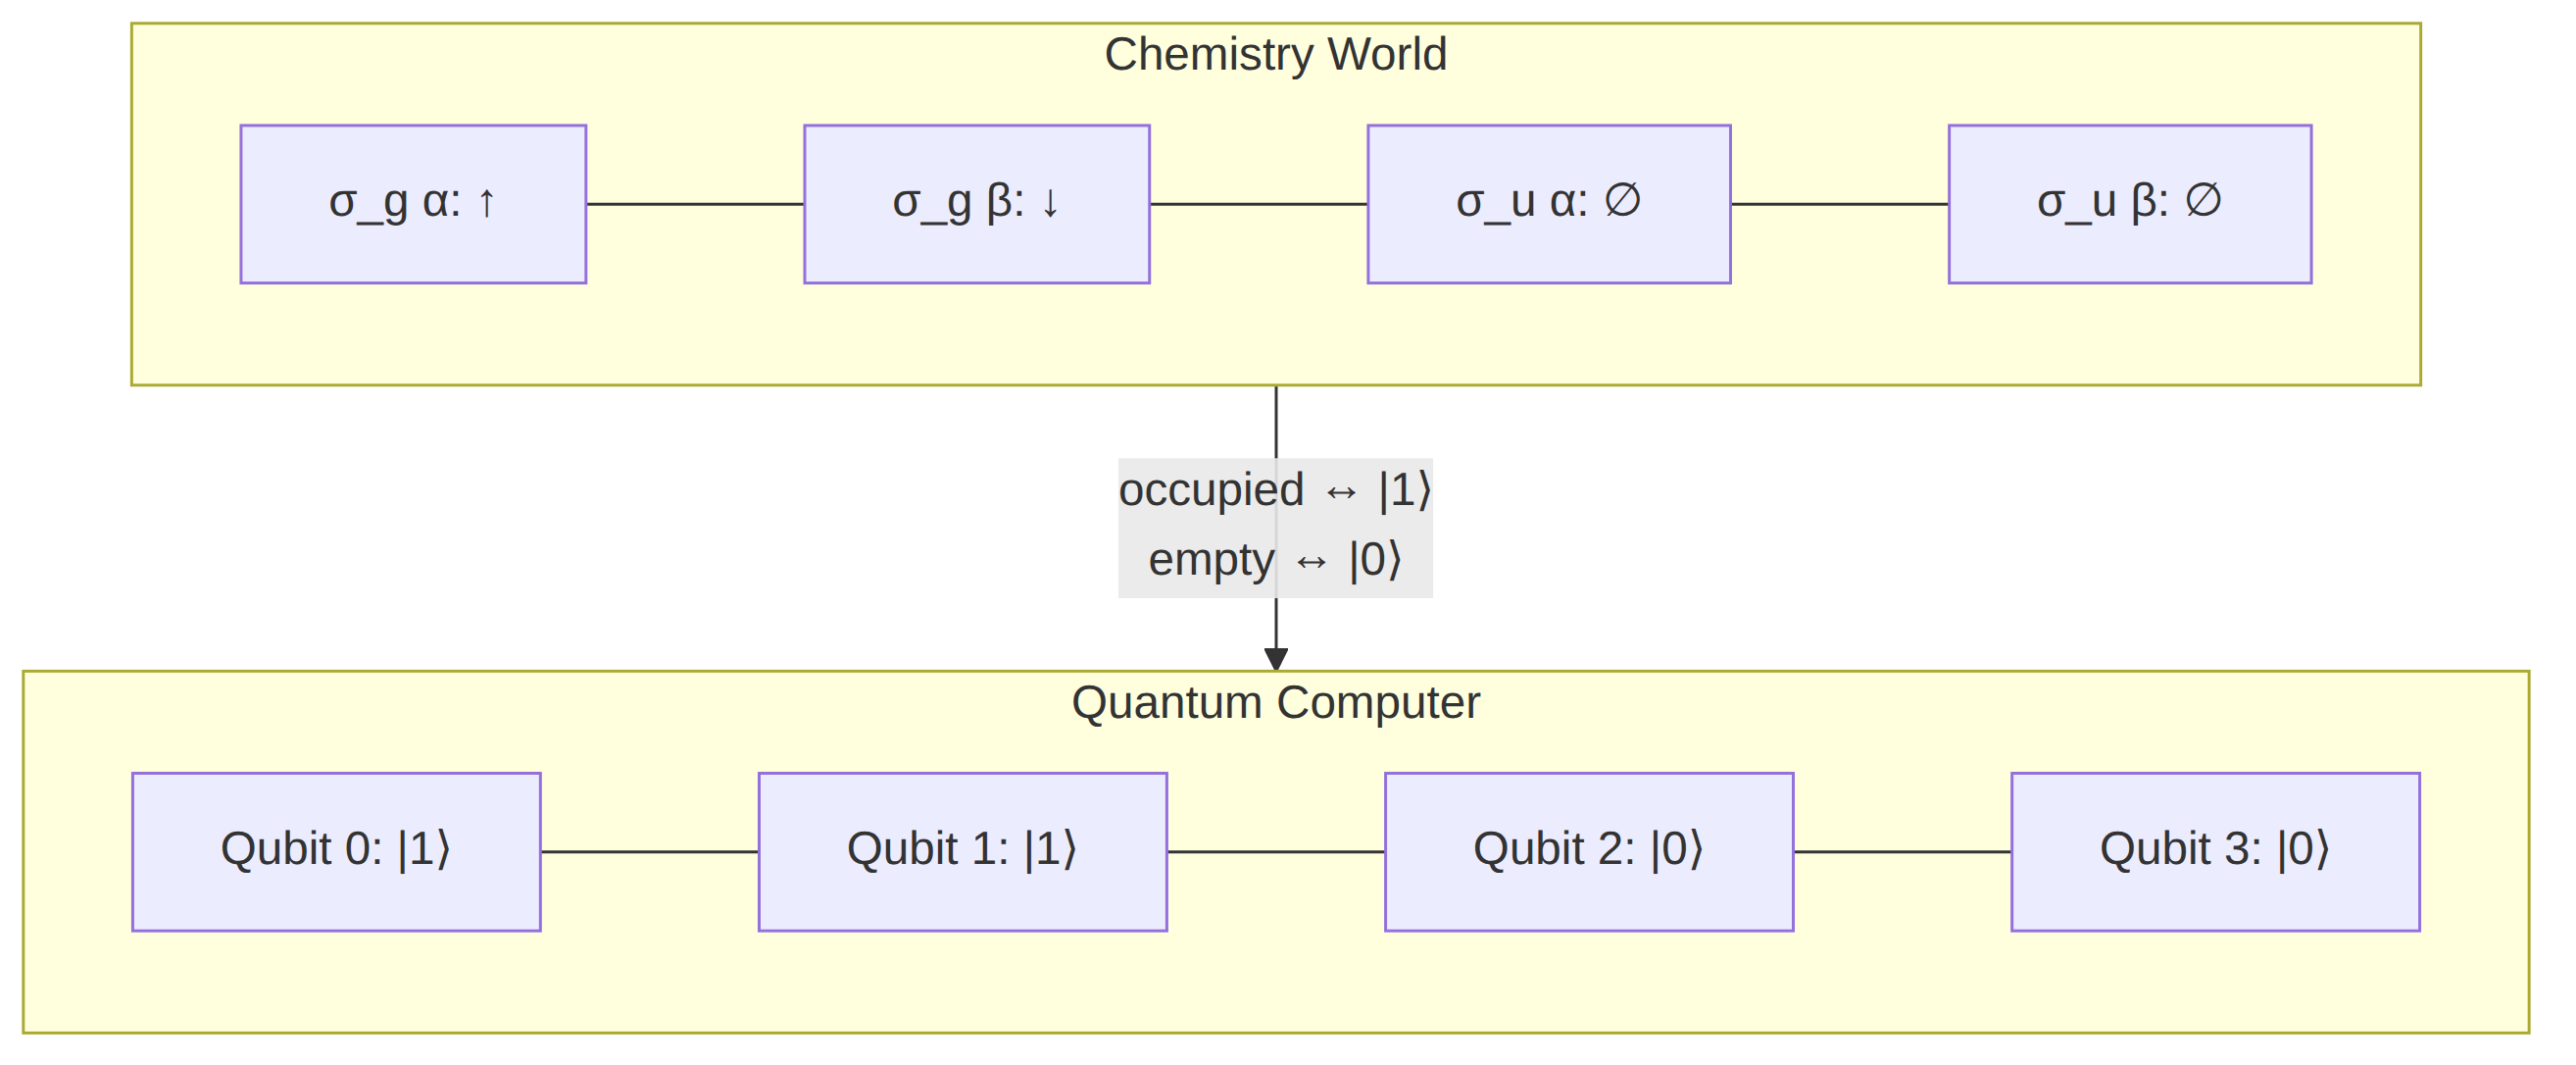
\includegraphics[keepaspectratio]{diagram-01.png}}

This mapping is correct for the \textbf{basis states}. But it is wrong
for the \textbf{operators}.

The creation operator \(a_2^\dagger\) does not simply flip qubit 2 from
\(\lvert 0\rangle\) to \(\lvert 1\rangle\). It must also check how many
electrons are in orbitals 0 and 1, and apply a minus sign if that count
is odd. This is the \textbf{fermion sign} --- the physical consequence
of the anti-commutation relations from Chapter 1.

Qubits don't anti-commute. If we flip qubit 2 without tracking the
fermion sign, we get the wrong quantum state. The encoding exists to
inject those signs.

\begin{center}\rule{0.5\linewidth}{0.5pt}\end{center}

\section{What Makes Electrons Different from
Qubits}\label{what-makes-electrons-different-from-qubits}

When we swap two electrons, the quantum state picks up a factor of
\(-1\):

\[\lvert A, B\rangle_{\text{fermion}} = -\lvert B, A\rangle_{\text{fermion}}\]

When we swap two qubits, nothing happens to the sign:

\[\lvert 0, 1\rangle_{\text{qubit}} = +\lvert 0, 1\rangle_{\text{qubit}}\]

This minus sign is not optional bookkeeping. It affects interference
patterns, bonding energies, and reaction rates. A faithful encoding must
reproduce it.

\begin{quote}
\textbf{The fermion sign, operationally:} Consider the occupation state
\(\lvert 1010\rangle\) (orbitals 0 and 2 occupied). To create an
electron in orbital 3, we apply \(a_3^\dagger\). No other occupied
orbitals lie between positions 2 and 3 (positions are counted from the
right), so the sign is \((-1)^0 = +1\). But to create an electron in
orbital 1, we must ``pass through'' the electron in orbital 2. The
anti-commutation rule charges one factor of \(-1\) for each occupied
orbital we pass: the sign is \((-1)^1 = -1\). This is the
\textbf{fermion sign} --- the net parity of occupied orbitals below the
target position. Every encoding must inject this sign into the qubit
representation.
\end{quote}

The mathematical statement is the anti-commutation relation:

\[a_p^\dagger a_q^\dagger = -a_q^\dagger a_p^\dagger\]

Creating an electron in orbital \(p\) and then orbital \(q\) gives the
opposite sign from creating in \(q\) then \(p\). On a qubit register,
flipping qubit \(p\) then qubit \(q\) gives the \emph{same} result as
flipping \(q\) then \(p\). The encoding must bridge this gap.

\begin{center}\rule{0.5\linewidth}{0.5pt}\end{center}

\section{Jordan--Wigner: The Z-Chain}\label{jordanwigner-the-z-chain}

The Jordan--Wigner encoding (1928) is the oldest and simplest solution.
Each qubit directly stores the occupation of one orbital --- same as the
``tempting idea'' --- but every creation or annihilation operator
carries a \textbf{chain of Z gates} that enforces the fermion sign.

\subsection{How the Z-chain works}\label{how-the-z-chain-works}

The \(Z\) gate acts on a qubit as a parity detector: - On
\(\lvert 0\rangle\) (empty orbital): \(Z\) gives \(+1\) - On
\(\lvert 1\rangle\) (occupied orbital): \(Z\) gives \(-1\)

To create an electron in orbital \(j\), we apply \(Z\) to every qubit
below \(j\) and then flip qubit \(j\). The product of all those \(Z\)
values gives \((-1)^{\text{count of occupied orbitals below } j}\) ---
exactly the fermion sign.

\pandocbounded{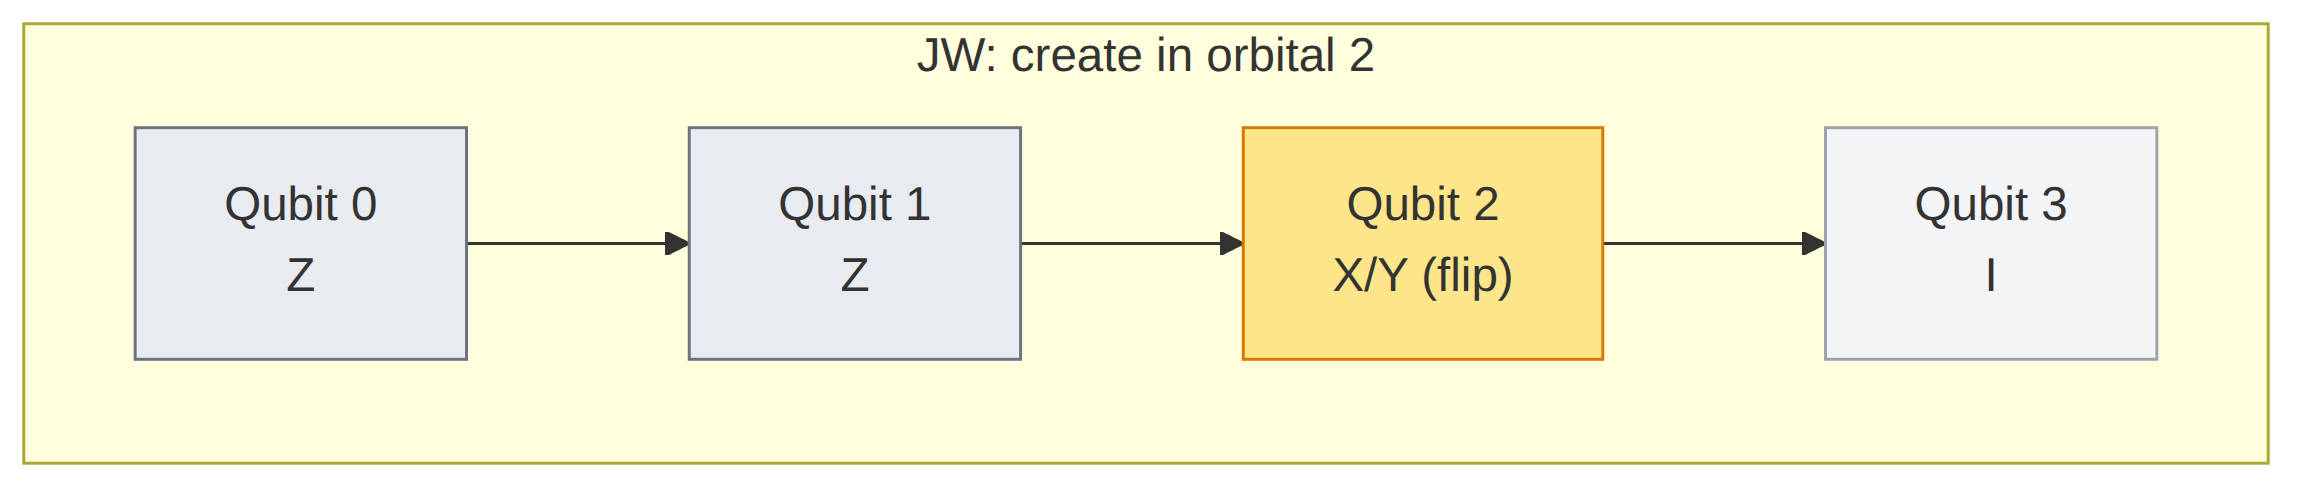
\includegraphics[keepaspectratio]{diagram-02.png}}

The Z-chain grows linearly: for orbital \(j\), we need \(j\) extra Z
operations. This is the \textbf{Pauli weight} of the encoded operator
--- the number of qubits it touches.

\subsection{JW Pauli weight for all four
orbitals}\label{jw-pauli-weight-for-all-four-orbitals}

\begin{longtable}[]{@{}cccccc@{}}
\toprule\noalign{}
Operator & q0 & q1 & q2 & q3 & Weight \\
\midrule\noalign{}
\endhead
\bottomrule\noalign{}
\endlastfoot
\(a_0^\dagger\) & \textbf{X/Y} & I & I & I & 1 \\
\(a_1^\dagger\) & Z & \textbf{X/Y} & I & I & 2 \\
\(a_2^\dagger\) & Z & Z & \textbf{X/Y} & I & 3 \\
\(a_3^\dagger\) & Z & Z & Z & \textbf{X/Y} & 4 \\
\end{longtable}

For a molecule with \(n\) spin-orbitals, the worst-case Pauli weight
under JW is \(n\). For FeMo-co (the iron-molybdenum cofactor of
nitrogenase --- the enzyme that fixes atmospheric nitrogen) with
\textasciitilde100 spin-orbitals, that's a chain of 99 Z gates for the
last orbital --- a very deep circuit on quantum hardware.

\subsection{When JW is the right
choice}\label{when-jw-is-the-right-choice}

Despite the linear scaling, JW excels when interactions are
\textbf{local} --- between neighboring orbitals. A hopping term
\(a_2^\dagger a_3 + a_3^\dagger a_2\) only needs a short Z-chain because
the two orbitals are adjacent. For 1D molecular chains or systems with
sequential orbital numbering, JW often has the lowest \emph{average}
weight even if its worst case is high.

\begin{center}\rule{0.5\linewidth}{0.5pt}\end{center}

\section{Bravyi--Kitaev: Partial Parity
Sums}\label{bravyikitaev-partial-parity-sums}

\subsection{The key insight}\label{the-key-insight}

The JW Z-chain answers the question: ``what is the parity (odd/even
count) of electrons in orbitals \(0, 1, \ldots, j-1\)?'' It answers this
by checking every orbital individually --- an \(O(n)\) scan.

What if some qubits pre-computed \textbf{partial parity sums}? Then we
could answer the question by reading \(O(\log n)\) qubits instead of
\(O(n)\).

This is the Bravyi--Kitaev (BK) encoding. It uses a data structure from
computer science --- the \textbf{Fenwick tree} (binary indexed tree) ---
to organize partial sums.

\subsection{How BK stores information}\label{how-bk-stores-information}

In JW, each qubit stores one orbital's occupation:

\pandocbounded{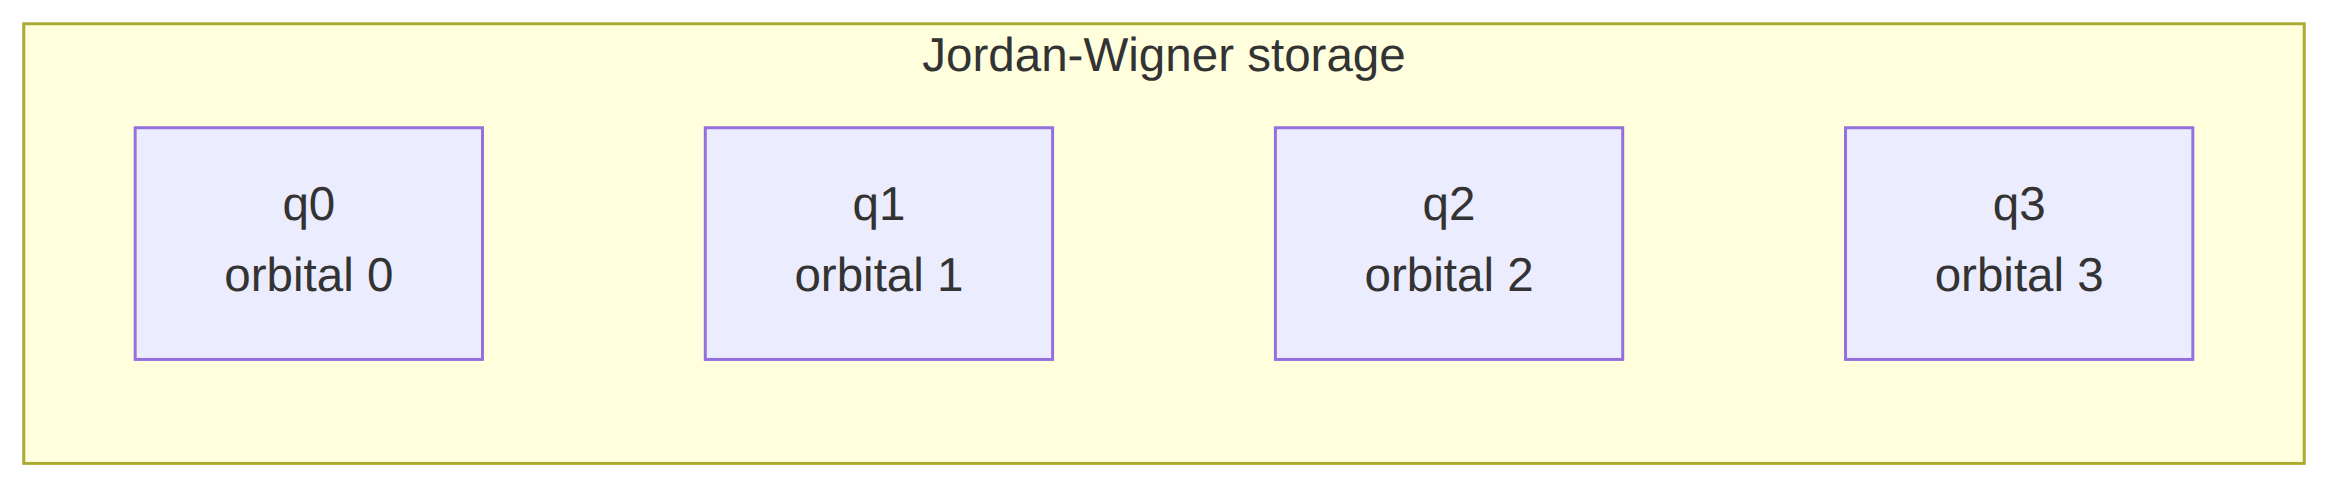
\includegraphics[keepaspectratio]{diagram-03.png}}

In BK, some qubits store \textbf{cumulative parity} --- the XOR of
multiple orbital occupations:

\pandocbounded{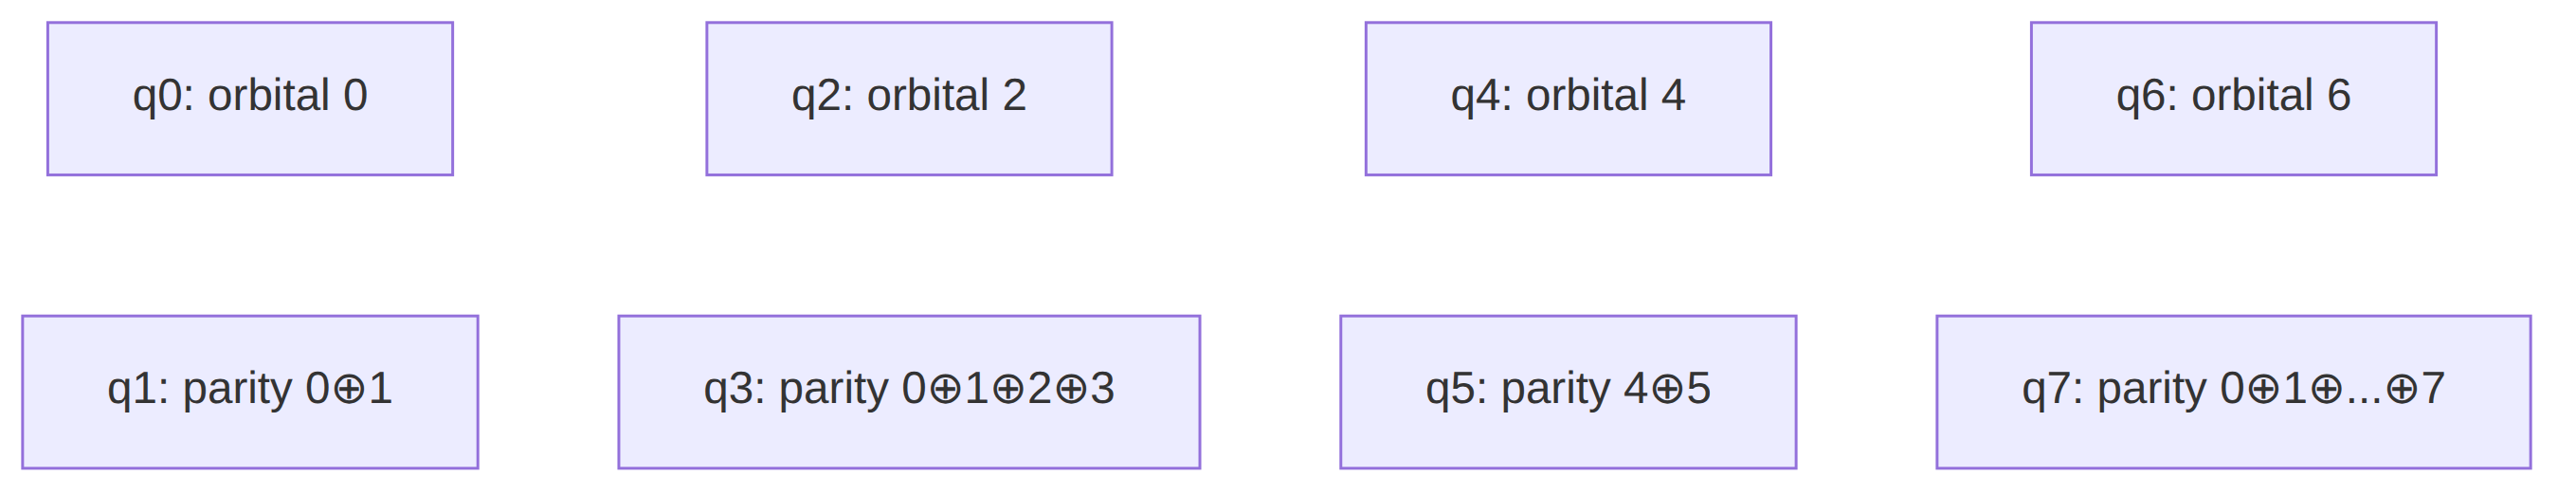
\includegraphics[keepaspectratio]{diagram-04.png}}

The pattern comes from a Fenwick tree. Each node stores the parity of
the orbitals in its subtree:

\pandocbounded{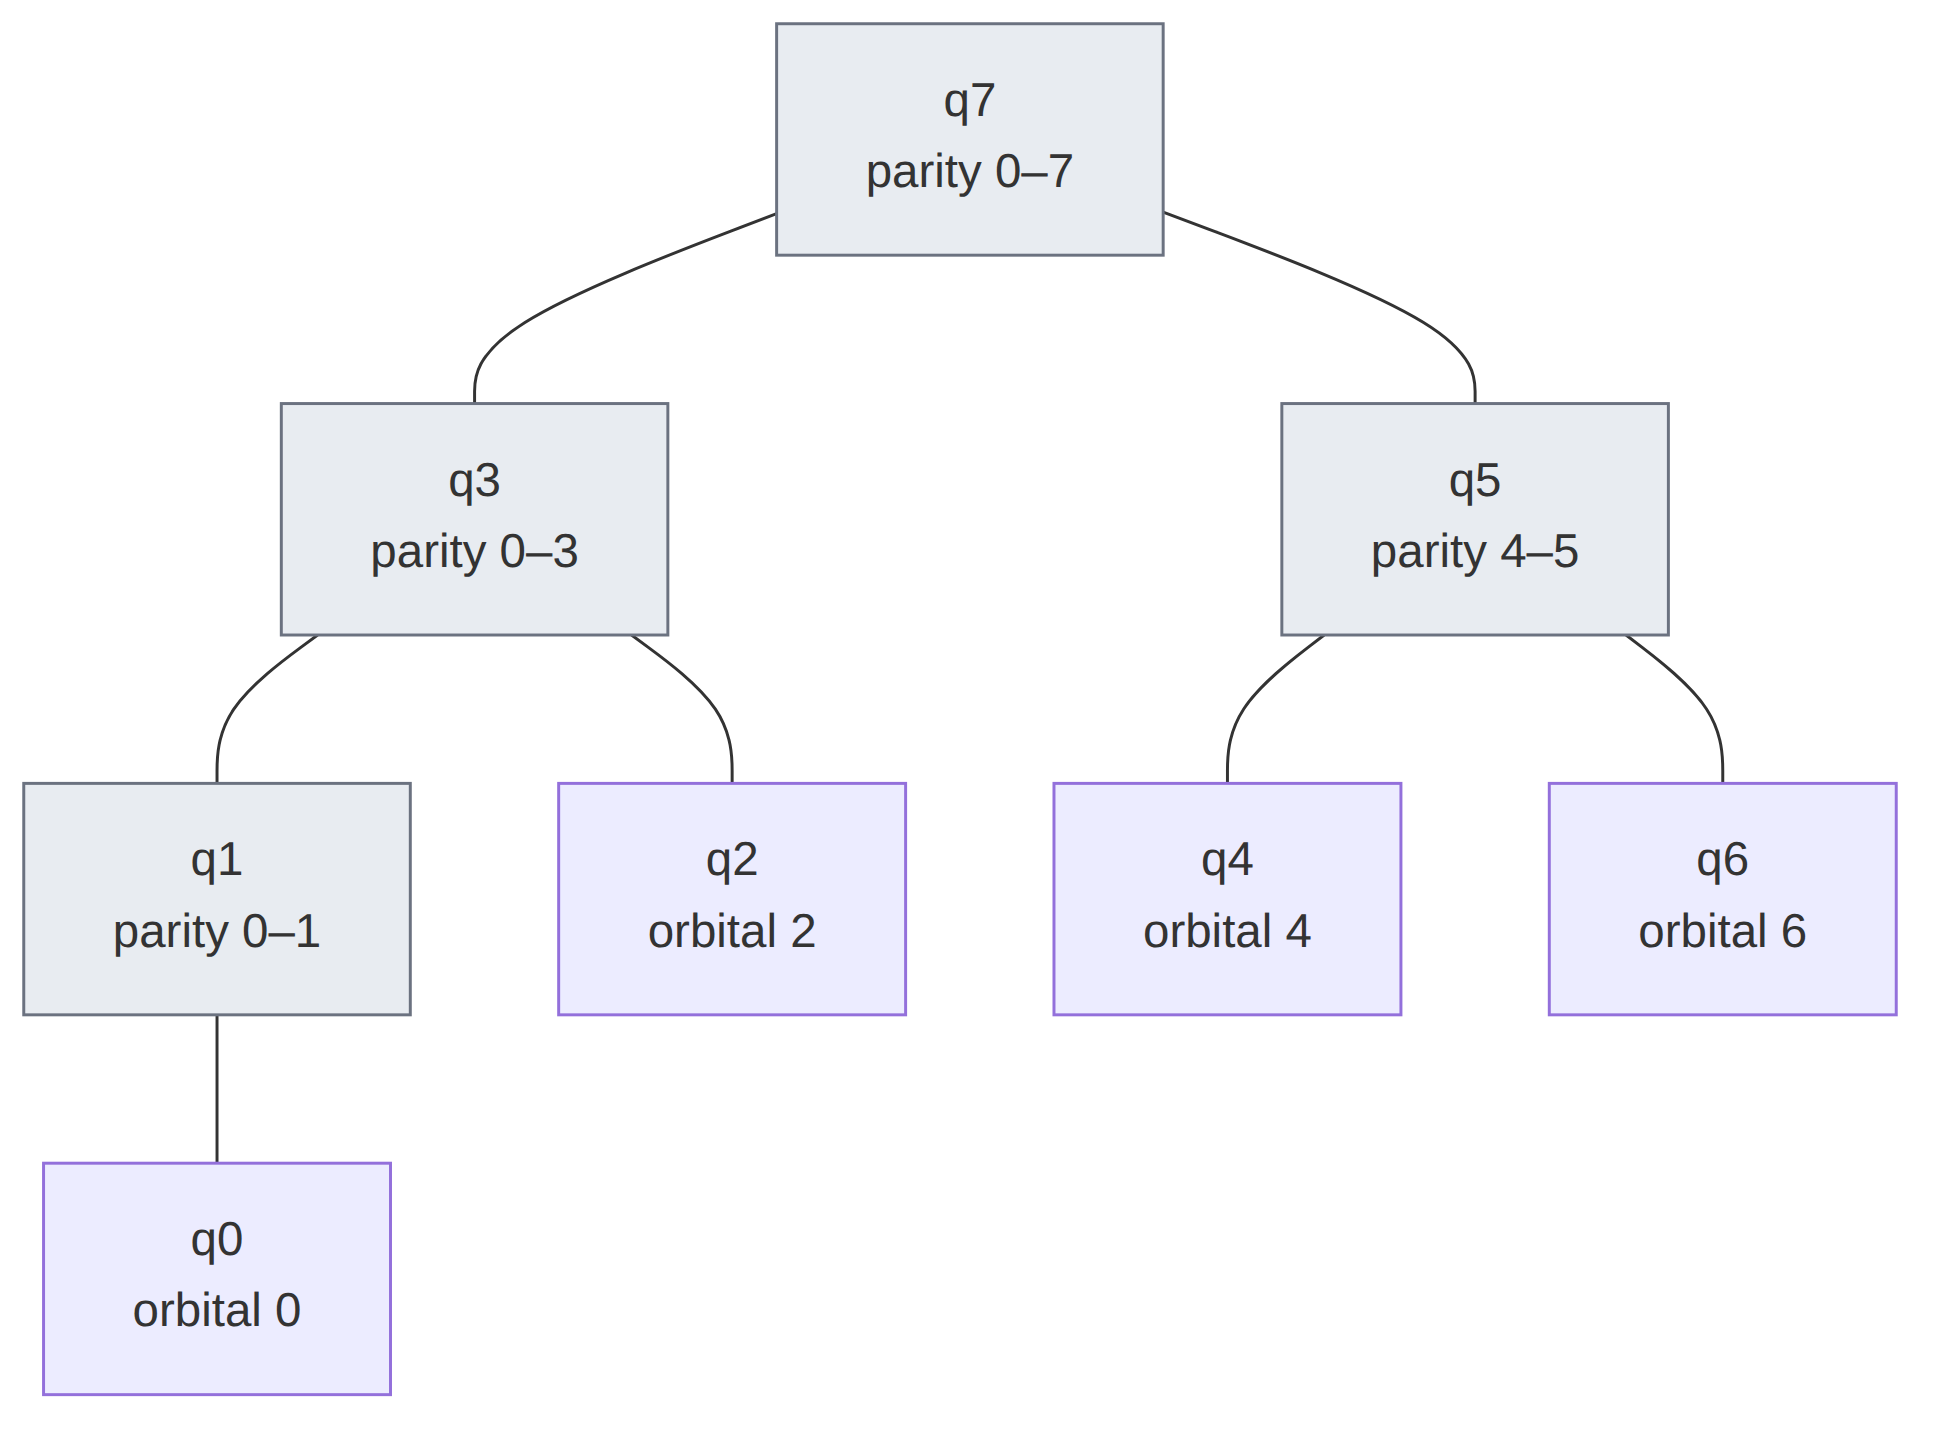
\includegraphics[keepaspectratio]{diagram-05.png}}

To find the parity of orbitals \(0\) through \(j-1\), you read the nodes
on the \emph{path} from node \(j\) up to the root --- at most
\(\log_2 n\) nodes.

\subsection{The three questions every encoding
answers}\label{the-three-questions-every-encoding-answers}

For each orbital \(j\), the encoding must answer three questions:

\begin{longtable}[]{@{}
  >{\raggedright\arraybackslash}p{(\linewidth - 4\tabcolsep) * \real{0.3333}}
  >{\raggedright\arraybackslash}p{(\linewidth - 4\tabcolsep) * \real{0.3333}}
  >{\raggedright\arraybackslash}p{(\linewidth - 4\tabcolsep) * \real{0.3333}}@{}}
\toprule\noalign{}
\begin{minipage}[b]{\linewidth}\raggedright
Question
\end{minipage} & \begin{minipage}[b]{\linewidth}\raggedright
JW answer
\end{minipage} & \begin{minipage}[b]{\linewidth}\raggedright
BK answer
\end{minipage} \\
\midrule\noalign{}
\endhead
\bottomrule\noalign{}
\endlastfoot
\textbf{Parity:} which qubits encode the fermion sign? & All qubits
\(0 \ldots j-1\) (\(O(n)\)) & \(\leq \log_2 n\) qubits on the Fenwick
path \\
\textbf{Update:} which qubits must change when orbital \(j\) is
filled/emptied? & Just qubit \(j\) & \(\leq \log_2 n\) ancestor
qubits \\
\textbf{Occupation:} which qubits reveal whether orbital \(j\) is
occupied? & Just qubit \(j\) & \(\leq \log_2 n\) descendant qubits \\
\end{longtable}

Every answer in BK involves at most \(\log_2 n\) qubits. That's the
advantage.

\subsection{Weight comparison at
scale}\label{weight-comparison-at-scale}

\begin{longtable}[]{@{}
  >{\centering\arraybackslash}p{(\linewidth - 6\tabcolsep) * \real{0.2500}}
  >{\centering\arraybackslash}p{(\linewidth - 6\tabcolsep) * \real{0.2500}}
  >{\centering\arraybackslash}p{(\linewidth - 6\tabcolsep) * \real{0.2500}}
  >{\centering\arraybackslash}p{(\linewidth - 6\tabcolsep) * \real{0.2500}}@{}}
\toprule\noalign{}
\begin{minipage}[b]{\linewidth}\centering
Spin-orbitals (\(n\))
\end{minipage} & \begin{minipage}[b]{\linewidth}\centering
JW worst-case weight
\end{minipage} & \begin{minipage}[b]{\linewidth}\centering
BK worst-case weight
\end{minipage} & \begin{minipage}[b]{\linewidth}\centering
Ratio
\end{minipage} \\
\midrule\noalign{}
\endhead
\bottomrule\noalign{}
\endlastfoot
4 & 4 & 3 & 1.3× \\
8 & 8 & 4 & 2× \\
16 & 16 & 5 & 3.2× \\
64 & 64 & 7 & 9× \\
100 & 100 & 7 & 14× \\
\end{longtable}

At 100 spin-orbitals, BK's worst-case operator touches 7 qubits while
JW's touches 100. On noisy hardware, this is the difference between a
feasible and an infeasible circuit.

\begin{center}\rule{0.5\linewidth}{0.5pt}\end{center}

\section{\texorpdfstring{Tree Encodings: Going Below
\(\log_2 n\)}{Tree Encodings: Going Below \textbackslash log\_2 n}}\label{tree-encodings-going-below-log_2-n}

\subsection{Beyond binary}\label{beyond-binary}

The Fenwick tree is a \emph{binary} tree --- each node has at most two
children. What if we used a \textbf{ternary} tree instead? Each internal
node would have three children, the tree would be shallower, and the
path lengths (and hence Pauli weights) would be shorter.

This is the insight behind the ternary tree encoding (Jiang et al.,
2020). It achieves worst-case Pauli weight \(O(\log_3 n)\) --- the best
known asymptotic scaling for any fermion-to-qubit encoding.

\pandocbounded{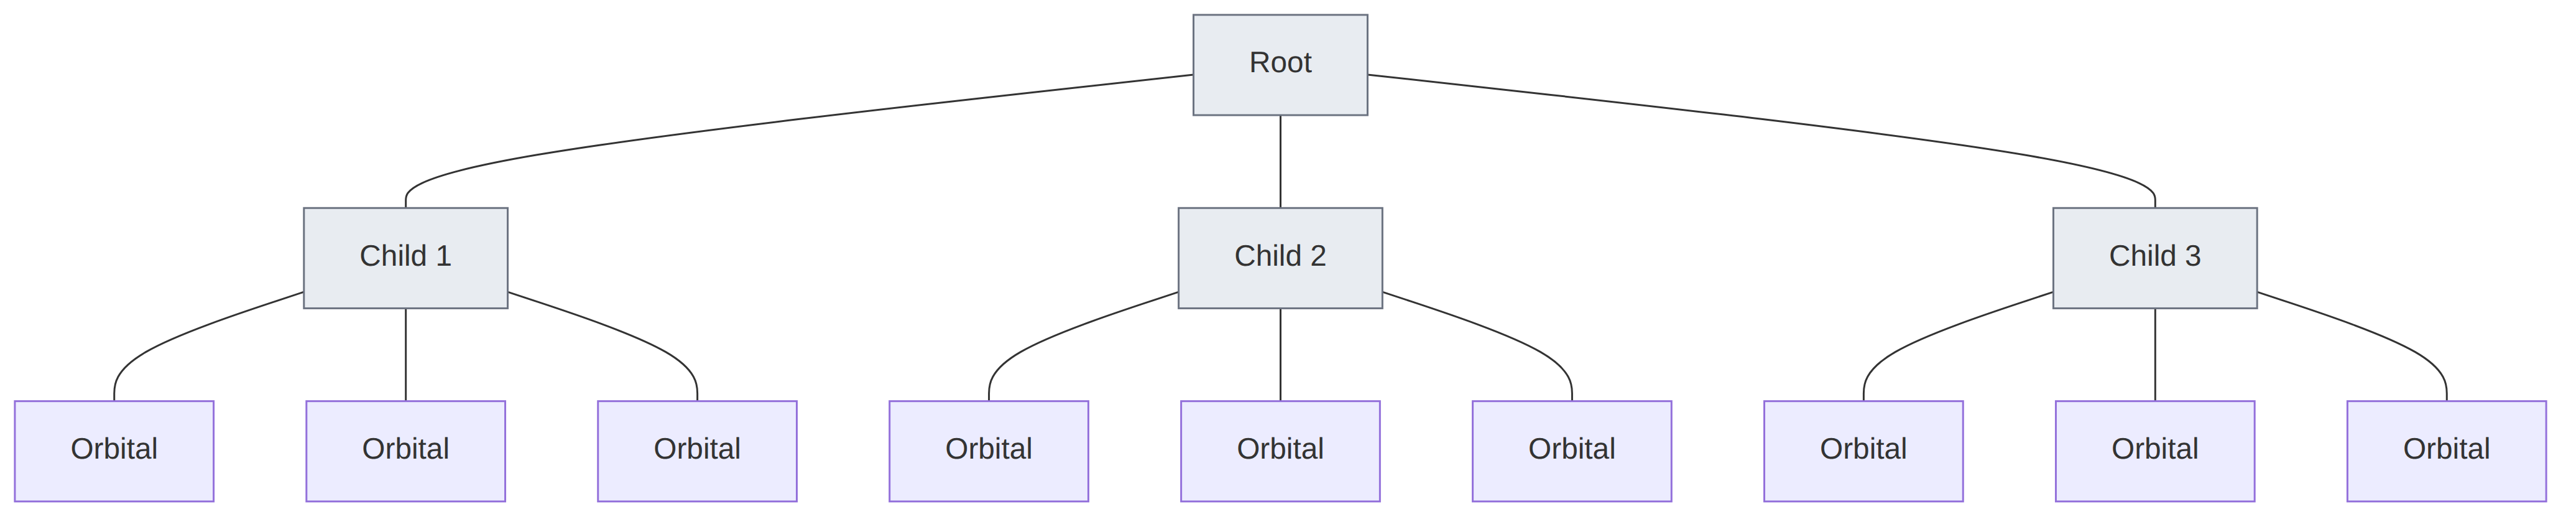
\includegraphics[keepaspectratio]{diagram-06.png}}

The three edges emerging from each node are labelled with the three
non-identity Pauli operators: X, Y, and Z. This labelling is what gives
the encoding its structure --- the Pauli string for each orbital is read
off by collecting edge labels on the path from root to leaf.

FockMap supports both balanced binary and balanced ternary tree
encodings, plus \textbf{arbitrary} tree topologies --- you can define
your own tree shape and derive a valid encoding from it.

\begin{center}\rule{0.5\linewidth}{0.5pt}\end{center}

\section{The Complete Picture}\label{the-complete-picture}

\pandocbounded{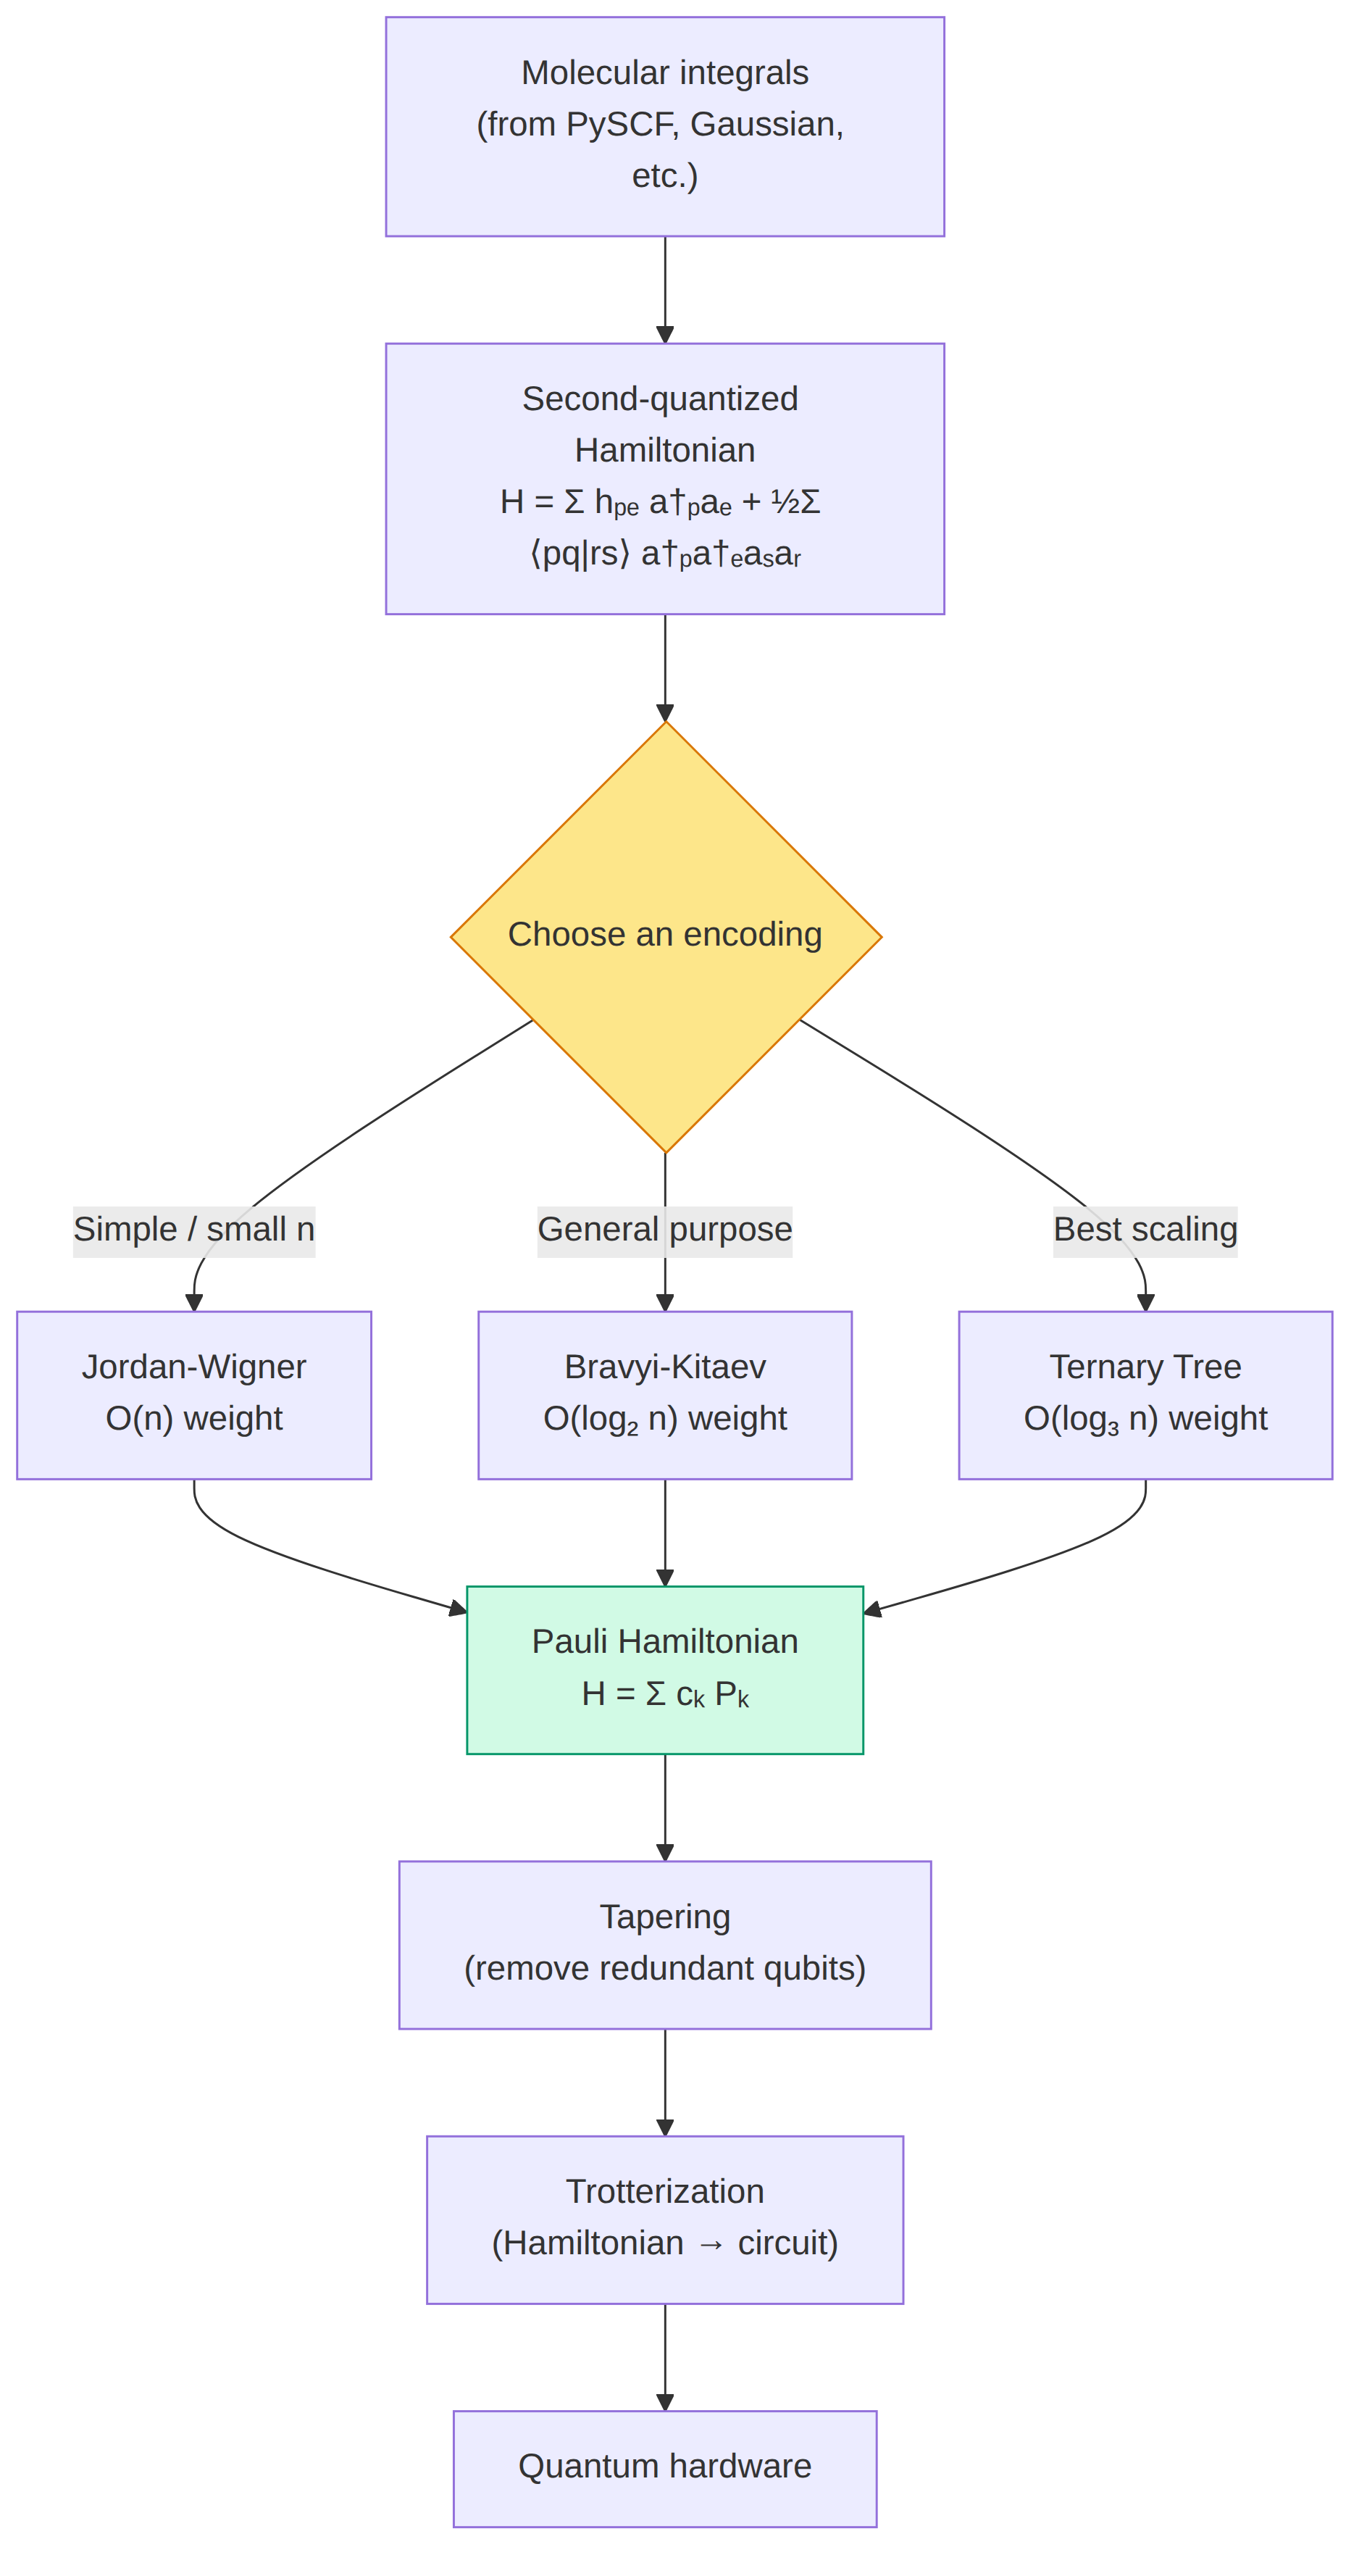
\includegraphics[keepaspectratio]{diagram-07.png}}

All six encodings in FockMap (JW, BK, Parity, balanced binary tree,
balanced ternary tree, Vlasov tree) produce the same output type: a
\texttt{PauliRegisterSequence}. They all give the same eigenvalues ---
the same physics. They differ only in how many qubits each Pauli string
touches, which determines circuit depth and measurement cost.

\begin{center}\rule{0.5\linewidth}{0.5pt}\end{center}

\section{One More Thing: Number Operators Stay
Cheap}\label{one-more-thing-number-operators-stay-cheap}

A reassuring fact: the \textbf{number operator}
\(n_j = a_j^\dagger a_j\) (which tests whether orbital \(j\) is
occupied) simplifies to just two terms under \emph{every} encoding:

\[n_j \;\mapsto\; \frac{1}{2}(I - Z_j) \quad \text{under JW}\]

That's Pauli weight 1 --- regardless of \(n\), regardless of encoding.
The Z-chains from the creation and annihilation operators cancel in the
product.

So while \emph{creating} or \emph{moving} electrons gets expensive under
JW (the Z-chains grow), simply \emph{counting} them stays cheap in all
encodings. The overhead only hits terms that change the electron
configuration --- and those are precisely the terms that represent
quantum correlations.

\begin{center}\rule{0.5\linewidth}{0.5pt}\end{center}

\section{Choosing an Encoding: A Decision
Guide}\label{choosing-an-encoding-a-decision-guide}

\begin{longtable}[]{@{}
  >{\raggedright\arraybackslash}p{(\linewidth - 4\tabcolsep) * \real{0.3333}}
  >{\raggedright\arraybackslash}p{(\linewidth - 4\tabcolsep) * \real{0.3333}}
  >{\raggedright\arraybackslash}p{(\linewidth - 4\tabcolsep) * \real{0.3333}}@{}}
\toprule\noalign{}
\begin{minipage}[b]{\linewidth}\raggedright
If your situation is\ldots{}
\end{minipage} & \begin{minipage}[b]{\linewidth}\raggedright
Use\ldots{}
\end{minipage} & \begin{minipage}[b]{\linewidth}\raggedright
Why
\end{minipage} \\
\midrule\noalign{}
\endhead
\bottomrule\noalign{}
\endlastfoot
Small molecule (\(n \leq 20\)) & Jordan--Wigner & Simplest, and the
weight overhead is manageable \\
1D chain / local Hamiltonian & Jordan--Wigner & Adjacent orbitals have
short Z-chains \\
Medium molecule (\(20 < n \leq 100\)) & Bravyi--Kitaev & \(O(\log_2 n)\)
weight saves significant circuit depth \\
Large molecule / all-to-all interactions & Ternary Tree &
\(O(\log_3 n)\) --- the best known scaling \\
Research / exploring custom topologies & Custom tree & FockMap supports
arbitrary tree shapes \\
\end{longtable}

In the next chapter, we will use all six encodings to build the complete
15-term H₂ Hamiltonian --- and see that they all agree.

\begin{center}\rule{0.5\linewidth}{0.5pt}\end{center}

\section{Key Takeaways}\label{key-takeaways-4}

\begin{itemize}
\tightlist
\item
  Electrons anti-commute; qubits don't. An encoding bridges this gap by
  injecting fermion signs into the qubit representation.
\item
  \textbf{Jordan--Wigner} uses a linear Z-chain: simple but \(O(n)\)
  weight.
\item
  \textbf{Bravyi--Kitaev} uses a Fenwick tree to pre-compute partial
  parities: \(O(\log_2 n)\) weight.
\item
  \textbf{Ternary tree} encodings go further: \(O(\log_3 n)\) weight ---
  the best known scaling.
\item
  All encodings produce the same physics (same eigenvalues). The choice
  affects only circuit cost.
\item
  Number operators are cheap (\(O(1)\)) in all encodings.
\end{itemize}

\section{Common Mistakes}\label{common-mistakes-4}

\begin{enumerate}
\def\labelenumi{\arabic{enumi}.}
\item
  \textbf{Forgetting fermion signs entirely.} Mapping occupation
  directly to qubits without an encoding gives classical (Hartree--Fock)
  results, not quantum results. The encoding is not optional --- it
  \emph{is} the quantum part.
\item
  \textbf{Assuming JW is always the worst.} For small systems and local
  interactions, JW often has the lowest \emph{average} weight. The
  \(O(n)\) scaling only becomes problematic at larger \(n\).
\item
  \textbf{Comparing raw term counts instead of Pauli weight.} All
  encodings produce the same number of Hamiltonian terms. The difference
  is in the weight (number of non-identity Paulis) per term, which
  determines CNOT count.
\end{enumerate}

\section{Exercises}\label{exercises-4}

\begin{enumerate}
\def\labelenumi{\arabic{enumi}.}
\item
  \textbf{Z-chain length.} For a system with 10 spin-orbitals, what is
  the JW Pauli weight of \(a_7^\dagger\)? What is the BK worst-case
  weight? (Use \(\lfloor \log_2 10 \rfloor + 1\).)
\item
  \textbf{Number operator.} Verify that the JW number operator
  \(n_j = \frac{1}{2}(I - Z_j)\) has eigenvalues 0 and 1 by applying it
  to \(\lvert 0 \rangle\) and \(\lvert 1 \rangle\).
\item
  \textbf{Tree branching.} If you used a 4-ary (quaternary) tree instead
  of ternary, what would the worst-case weight scaling be? Would it be
  better or worse than ternary, and why might it not work as easily?
\end{enumerate}

\section{Further Reading}\label{further-reading-4}

\begin{itemize}
\tightlist
\item
  Jordan, P. and Wigner, E. ``Über das Paulische Äquivalenzverbot.''
  \emph{Z. Physik} 47, 631 (1928). The original encoding --- a
  mathematical trick for mapping spin chains that found its second life
  in quantum computing 77 years later.
\item
  Aspuru-Guzik, A., Dutoi, A. D., Love, P. J., and Head-Gordon, M.
  ``Simulated Quantum Computation of Molecular Energies.''
  \emph{Science} 309, 1704 (2005). The paper that launched quantum
  computational chemistry: showed that the Jordan--Wigner encoding could
  be plugged into a quantum phase estimation algorithm to compute
  molecular ground-state energies. Before this work, JW was a
  mathematical curiosity; after it, an entire field was born.
\item
  Seeley, J. T., Richard, M. J., and Love, P. J. ``The Bravyi--Kitaev
  transformation for quantum computation of electronic structure.''
  \emph{J. Chem. Phys.} 137, 224109 (2012). Formalized the
  \textbf{index-set framework} --- the three set-valued functions
  (Update, Parity, Occupation) that unify JW, BK, and Parity under a
  single abstraction. This is the framework that FockMap's
  \texttt{EncodingScheme} type directly implements.
\item
  Bravyi, S. B. and Kitaev, A. Yu. ``Fermionic Quantum Computation.''
  \emph{Ann. Phys.} 298, 210 (2002). The logarithmic-weight encoding
  using Fenwick trees.
\item
  Jiang, Z. et al.~``Optimal fermion-to-qubit mapping via ternary
  trees.'' \emph{PRX Quantum} 1, 010306 (2020). The ternary tree
  encoding with optimal asymptotic scaling.
\end{itemize}

\begin{center}\rule{0.5\linewidth}{0.5pt}\end{center}

\chapter{Chapter 6: Building the Qubit
Hamiltonian}\label{chapter-6-building-the-qubit-hamiltonian}

\emph{This is where the pipeline pays off. We take the integral tables
from Chapter 3, the encoding from Chapter 5, and produce the actual
qubit Hamiltonian --- the object that a quantum computer will simulate.}

\section{In This Chapter}\label{in-this-chapter-5}

\begin{itemize}
\tightlist
\item
  \textbf{What you'll learn:} Why the distinction between diagonal and
  off-diagonal Hamiltonian terms is the central idea of quantum
  simulation, how to systematically encode fermionic terms into Pauli
  strings, and how to read the resulting 15-term H₂ Hamiltonian as a map
  of classical vs quantum physics.
\item
  \textbf{Why this matters:} This is the exact object used by VQE, QPE,
  and every other quantum simulation algorithm. Understanding its
  structure --- which parts are classical, which parts are quantum ---
  is the key to understanding why quantum computing matters for
  chemistry.
\item
  \textbf{Prerequisites:} Chapters 1--5 (integrals, notation,
  spin-orbitals, gates, encoding concepts).
\end{itemize}

\begin{center}\rule{0.5\linewidth}{0.5pt}\end{center}

\section{The Density Matrix: Where Classical Ends and Quantum
Begins}\label{the-density-matrix-where-classical-ends-and-quantum-begins}

Before we compute anything, we need to understand what we're looking for
--- because the structure of the qubit Hamiltonian will tell us exactly
where classical physics ends and quantum physics begins.

\subsection{Classical: a probability
distribution}\label{classical-a-probability-distribution}

If electrons were classical particles, we could describe their state as
a \textbf{probability distribution} over configurations:

\[\text{Prob}(\lvert 1100\rangle) = 0.95, \quad \text{Prob}(\lvert 0011\rangle) = 0.03, \quad \text{Prob}(\lvert 1010\rangle) = 0.02, \quad \ldots\]

This tells us: ``if we look, there's a 95\% chance both electrons are in
the bonding orbital, a 3\% chance both are in the antibonding orbital,''
and so on. The expected energy is just a weighted average:
\(E_{\text{classical}} = \sum_i p_i \, E_i\).

Mathematically, this is a \textbf{diagonal} density matrix --- numbers
along the diagonal (the probabilities) and zeros everywhere else:

\[\rho_{\text{classical}} = \begin{pmatrix}
0.95 & 0 & 0 & \cdots \\
0 & 0.03 & 0 & \cdots \\
0 & 0 & 0.02 & \cdots \\
\vdots & \vdots & \vdots & \ddots
\end{pmatrix}\]

Hartree--Fock is essentially this picture: the electrons are in
\(\lvert 1100\rangle\) with probability 1. One non-zero diagonal entry.
No mixing, no uncertainty beyond what's already baked into the orbital
structure.

\subsection{Quantum: coherences change
everything}\label{quantum-coherences-change-everything}

A quantum state is fundamentally different. The ground state of H₂ is
not ``95\% chance of \(\lvert 1100\rangle\).'' It is a
\textbf{superposition}:

\[\lvert\Psi\rangle = c_1\lvert 1100\rangle + c_2\lvert 0011\rangle + \cdots\]

The density matrix \(\rho = \lvert\Psi\rangle\langle\Psi\rvert\) now has
off-diagonal elements:

\[\rho_{\text{quantum}} = \begin{pmatrix}
\lvert c_1\rvert^2 & c_1 c_2^* & \cdots \\
c_2 c_1^* & \lvert c_2\rvert^2 & \cdots \\
\vdots & \vdots & \ddots
\end{pmatrix}\]

The diagonal entries \(\lvert c_i\rvert^2\) are probabilities --- same
as the classical case. But the off-diagonal entries \(c_i c_j^*\) are
\textbf{coherences}. They have no classical analogue. They encode the
\emph{phase relationships} between configurations --- the interference
patterns that allow the quantum state to have a lower energy than any
classical mixture of the same configurations.

\begin{quote}
\textbf{The off-diagonal elements of the density matrix are the quantum
difference.}
\end{quote}

A classical mixture with the same occupation probabilities would have a
\emph{higher} energy. But why? To see this, we need to understand how
energy is actually computed from a density matrix.

\subsection{The trace: a machine for computing
averages}\label{the-trace-a-machine-for-computing-averages}

The expected energy of a system in state \(\rho\) is:

\[\langle H \rangle = \text{Tr}(\rho H)\]

The \textbf{trace} of a matrix is the sum of its diagonal elements. But
\(\text{Tr}(\rho H)\) is not just summing the diagonal of \(\rho\) ---
it's summing the diagonal of the \emph{product} \(\rho H\). And the
product of two matrices mixes their rows and columns:

\[\text{Tr}(\rho H) = \sum_i (\rho H)_{ii} = \sum_i \sum_j \rho_{ij} H_{ji}\]

We can split this into two parts:

\[\langle H \rangle = \underbrace{\sum_i \rho_{ii} H_{ii}}_{\text{classical}} + \underbrace{\sum_{i \neq j} \rho_{ij} H_{ji}}_{\text{quantum}}\]

The first sum is the \textbf{classical energy}: each configuration's
probability times its diagonal energy. This is what Hartree--Fock
computes --- a single \(\rho_{ii} = 1\), everything else zero, and
\(\langle H \rangle = H_{ii}\).

The second sum is the \textbf{quantum correction}: the off-diagonal
elements of \(\rho\) (the coherences) multiplied by the off-diagonal
elements of \(H\) (the exchange terms). This sum can be \emph{negative}
--- it can lower the energy below the classical minimum. This is the
correlation energy.

But notice: for this second sum to be nonzero, \textbf{both} \(\rho\)
and \(H\) must have off-diagonal elements. If the Hamiltonian is
diagonal (no X or Y terms), then \(H_{ji} = 0\) for \(i \neq j\), and
the quantum correction vanishes regardless of what \(\rho\) looks like.
If \(\rho\) is diagonal (no coherences), the correction vanishes
regardless of \(H\).

The trace formula makes the thesis mathematically precise: quantum
advantage requires off-diagonal elements in \emph{both} the state and
the Hamiltonian, working together through the trace to produce an energy
that no diagonal (classical) computation can reach.

\subsection{What generates coherences?}\label{what-generates-coherences}

\textbf{Diagonal Hamiltonian terms} (built from I and Z only) do not mix
configurations. They assign energies --- ``configuration
\(\lvert 1100\rangle\) costs this much, configuration
\(\lvert 0011\rangle\) costs that much.'' Under time evolution, they
rotate phases but never create superpositions. A diagonal Hamiltonian
cannot generate off-diagonal density matrix elements. Its ground state
is always a single configuration.

\textbf{Off-diagonal Hamiltonian terms} (containing X or Y) \emph{mix}
configurations. They connect \(\lvert 1100\rangle\) to
\(\lvert 0011\rangle\), creating the superposition --- the coherences
--- that lower the energy below the classical minimum.

The chain of implications is absolute:

\[\text{No off-diagonal } H \;\Rightarrow\; \text{no coherences in } \rho \;\Rightarrow\; \text{no correlation energy} \;\Rightarrow\; \text{HF is exact} \;\Rightarrow\; \text{no quantum computer needed}\]

\subsection{What this means for
encoding}\label{what-this-means-for-encoding}

Now we can state precisely what the encoding must accomplish:

The \textbf{diagonal part} of the Hamiltonian (orbital energies, Coulomb
repulsion) is cheap. It maps to I and Z Pauli operators, diagonal in the
computational basis. Measuring them is trivial. Simulating their time
evolution requires only single-qubit Z-rotations. No entanglement, no
deep circuits.

The \textbf{off-diagonal part} (exchange interactions) is expensive. It
maps to X and Y Pauli operators, which flip qubits and create
entanglement. Simulating these terms requires multi-qubit gates --- CNOT
staircases, as we'll see in the Circuits stage (Chapters 14--17). The
Pauli weight of these off-diagonal terms directly determines the circuit
depth.

\textbf{The encoding choice determines the cost of the off-diagonal
terms.} JW, BK, and tree encodings all produce the same diagonal terms
--- they differ only in how they handle the Z-chains that accompany the
off-diagonal X/Y operators.

\textbf{This is the thesis of the entire book:} the correlation energy
lives in the off-diagonal coherences of the density matrix, and the
encoding determines how expensive it is to create and maintain those
coherences on quantum hardware.

With this lens in place, let's build the Hamiltonian and see the
structure emerge.

\begin{center}\rule{0.5\linewidth}{0.5pt}\end{center}

\section{What We Have and What We'll
Do}\label{what-we-have-and-what-well-do}

Chapters 1--4 gave us everything we need:

\begin{itemize}
\tightlist
\item
  \textbf{The chemistry} (Chapter 1): H₂ in STO-3G, 4 spin-orbitals, the
  second-quantized Hamiltonian.
\item
  \textbf{The notation} (Chapter 2): physicist's convention, the
  conversion rule, the traps to avoid.
\item
  \textbf{The numbers} (Chapter 3): complete spin-orbital integral
  tables and a coefficient factory in F\#.
\item
  \textbf{The quantum computer} (Chapter 4): qubits, gates, CNOT cost,
  and the \(2(w-1)\) formula.
\item
  \textbf{The encoding} (Chapter 5): Jordan--Wigner's Z-chain mechanism
  for translating fermionic operators to Pauli strings.
\end{itemize}

The procedure from here is mechanical. Once you see it done for one
term, you can do it for any term, for any molecule, in any encoding. The
insight is behind us; what remains is careful bookkeeping.

\begin{center}\rule{0.5\linewidth}{0.5pt}\end{center}

\section{The Recipe}\label{the-recipe}

\pandocbounded{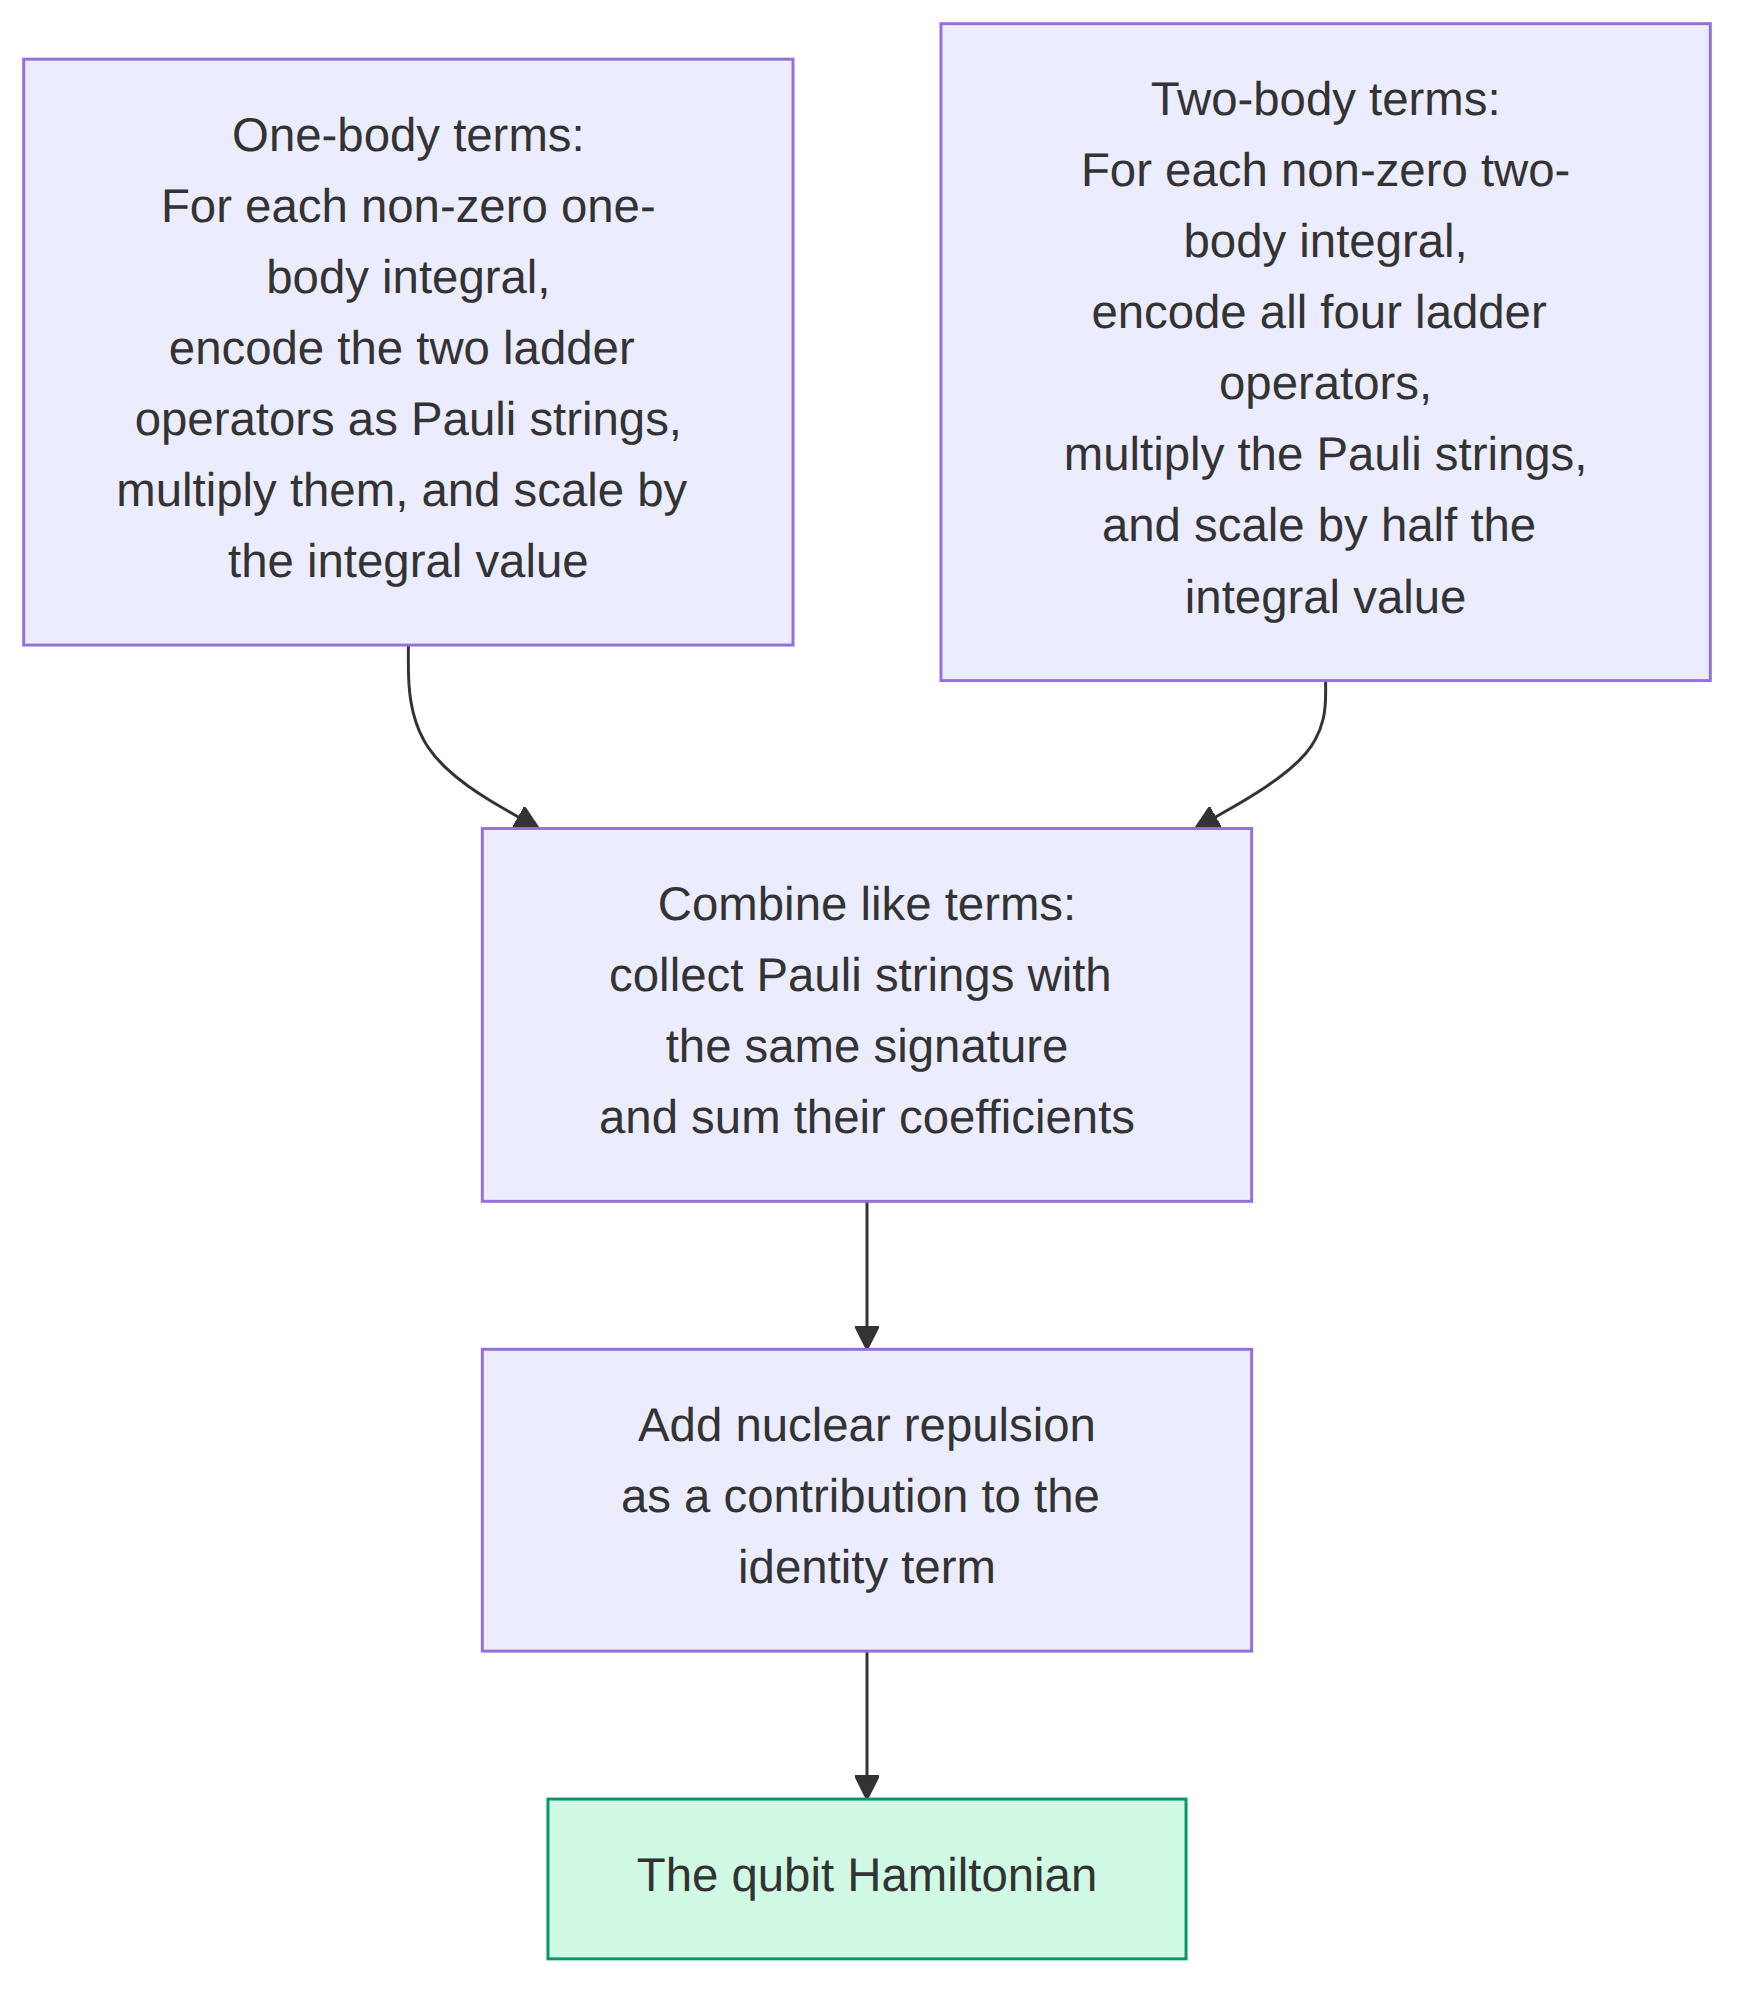
\includegraphics[keepaspectratio]{diagram-08.png}}

FockMap does this symbolically --- no matrices, no floats in the
intermediate algebra. We'll work through one representative term by
hand, then show the complete result.

\subsection{One-body terms: number
operators}\label{one-body-terms-number-operators}

The non-zero one-body integrals for H₂ are all diagonal (Chapter 3):
\(h_{00} = h_{11} = -1.2563\) Ha and \(h_{22} = h_{33} = -0.4719\) Ha.
Under Jordan--Wigner, the number operator simplifies --- the Z-chains
cancel:

\[\hat{n}_j = a_j^\dagger a_j = \frac{1}{2}(I - Z_j)\]

Weight 1, regardless of system size. The one-body Hamiltonian produces
five terms --- all diagonal, all classical:

\begin{longtable}[]{@{}ccl@{}}
\toprule\noalign{}
Pauli term & Coefficient (Ha) & Origin \\
\midrule\noalign{}
\endhead
\bottomrule\noalign{}
\endlastfoot
\(IIII\) & \(-1.7282\) & Sum of all orbital energies, halved \\
\(IIIZ\) & \(+0.6282\) & \(-h_{00}/2\) (energy of
\(\sigma_g, \alpha\)) \\
\(IIZI\) & \(+0.6282\) & \(-h_{11}/2\) (energy of
\(\sigma_g, \beta\)) \\
\(IZII\) & \(+0.2359\) & \(-h_{22}/2\) (energy of
\(\sigma_u, \alpha\)) \\
\(ZIII\) & \(+0.2359\) & \(-h_{33}/2\) (energy of
\(\sigma_u, \beta\)) \\
\end{longtable}

All I and Z. No off-diagonal terms. No coherences generated. If this
were the whole Hamiltonian, a laptop would suffice.

\subsection{Two-body terms: one by
hand}\label{two-body-terms-one-by-hand}

Consider the Coulomb repulsion between two electrons in \(\sigma_g\)
with opposite spins:
\(\frac{1}{2}\langle 01 \mid 01\rangle\; a_0^\dagger a_1^\dagger a_1 a_0\),
with integral value \(0.6745\) Ha.

Encode each operator under JW, multiply the four Pauli strings, and
simplify. Three observations make the algebra tractable: the Z-chains
cancel (\(Z_0 \cdot Z_0 = I\)), and each raising-lowering pair
simplifies via \((X - iY)(X + iY) = 2(I - Z)\).

\[a_0^\dagger a_1^\dagger a_1 a_0 = \frac{1}{4}(IIII - IIIZ - IIZI + IIZZ)\]

Scaled by the integral: four diagonal Pauli contributions. This is a
Coulomb term --- pure classical electrostatics, no off-diagonal
structure. Exactly as the density matrix framework predicted.

The \textbf{exchange} integrals \(\langle 02 \mid 20\rangle\) tell a
different story. They produce terms like
\(a_0^\dagger a_2^\dagger a_0 a_2\), where electrons swap orbitals.
Under JW, these don't simplify to pure Z --- they leave XX and YY Pauli
operators. These are the off-diagonal terms. They generate coherences.
They produce the correlation energy.

Let's see this happen explicitly.

\subsection{One exchange term, fully
expanded}\label{one-exchange-term-fully-expanded}

Consider
\(\frac{1}{2}\langle 02 \mid 20\rangle\; a_0^\dagger a_2^\dagger a_2 a_0\),
with integral value \(\langle 02 \mid 20\rangle = 0.1809\) Ha. This is
an exchange integral --- electron 1 scatters from orbital 0 to orbital
2, electron 2 scatters from orbital 2 to orbital 0.

\textbf{Encode under Jordan--Wigner:}

\[a_0^\dagger = \frac{1}{2}(X_0 - iY_0) \otimes I_1 \otimes I_2 \otimes I_3\]

\[a_2^\dagger = \frac{1}{2}\,Z_0 Z_1 \otimes (X_2 - iY_2) \otimes I_3\]

\[a_2 = \frac{1}{2}\,Z_0 Z_1 \otimes (X_2 + iY_2) \otimes I_3\]

\[a_0 = \frac{1}{2}(X_0 + iY_0) \otimes I_1 \otimes I_2 \otimes I_3\]

Note: \(a_2^\dagger\) has a Z-chain of length 2 (\(Z_0 Z_1\)), not
length 1.

\textbf{Multiply.}

\[a_0^\dagger a_2^\dagger a_2 a_0 = \frac{1}{16}(X_0 - iY_0)\,Z_0 Z_1(X_2 - iY_2)\,Z_0 Z_1(X_2 + iY_2)\,(X_0 + iY_0)\]

\textbf{Simplify.} The Z-chains cancel on qubits 0 and 1:
\(Z_0 Z_0 = I\), \(Z_1 Z_1 = I\). The qubit-2 pair simplifies as before:
\((X_2 - iY_2)(X_2 + iY_2) = 2(I - Z_2)\). But now qubit 0 has something
new:

\[(X_0 - iY_0) \cdot (X_0 + iY_0) = 2(I - Z_0)\]

Wait --- that's the same identity as the Coulomb case. So where do the
XX/YY terms come from?

They come from a \emph{different} index combination. Consider instead:

\[\frac{1}{2}\langle 02 \mid 02\rangle\; a_0^\dagger a_2^\dagger a_0 a_2\]

Here the operator ordering is \(a_0^\dagger a_2^\dagger a_0 a_2\) ---
note the annihilation operators are \(a_0 a_2\), not \(a_2 a_0\). When
we encode and multiply:

\[a_0^\dagger a_2^\dagger a_0 a_2 = \frac{1}{16}(X_0 - iY_0)\,Z_0 Z_1(X_2 - iY_2)\,(X_0 + iY_0)\,Z_0 Z_1(X_2 + iY_2)\]

Now the Z-chains don't cancel cleanly --- the \((X_0 + iY_0)\) sits
\emph{between} the two Z₀ factors instead of outside them. Expanding
qubit 0:

\[(X_0 - iY_0)\,Z_0\,(X_0 + iY_0)\,Z_0\]

Using \(X Z = -iY\), \(Y Z = iX\), and carefully tracking the phases,
this produces terms proportional to \(X_0 X_2\), \(Y_0 Y_2\),
\(X_0 Y_2\), and \(Y_0 X_2\) --- the off-diagonal Pauli operators.

The full expansion (which FockMap performs symbolically) yields
contributions to \(XXYY\), \(XYYX\), \(YXXY\), and \(YYXX\) ---
precisely the four exchange terms in the final Hamiltonian, with
coefficient \(\pm 0.1744\).

\begin{quote}
\textbf{What just happened:} When the annihilation operators are in a
different order from the creation operators (electrons change orbitals),
the Z-chains interleave with the X/Y flips instead of cancelling. The
result is an off-diagonal Pauli string --- exactly the structure that
generates coherences in the density matrix.
\end{quote}

\begin{center}\rule{0.5\linewidth}{0.5pt}\end{center}

\section{The Complete 15-Term
Hamiltonian}\label{the-complete-15-term-hamiltonian}

After processing all 32 non-zero two-body integrals, combining like
terms, and adding \(V_{nn} = 0.7151\) Ha:

\begin{longtable}[]{@{}cccl@{}}
\toprule\noalign{}
\# & Pauli String & Coefficient (Ha) & Character \\
\midrule\noalign{}
\endhead
\bottomrule\noalign{}
\endlastfoot
1 & \(IIII\) & \(-1.0704\) & Energy offset \\
2 & \(IIIZ\) & \(-0.0958\) & Orbital energy \\
3 & \(IIZI\) & \(-0.0958\) & Orbital energy \\
4 & \(IZII\) & \(+0.3021\) & Orbital energy \\
5 & \(ZIII\) & \(+0.3021\) & Orbital energy \\
6 & \(IIZZ\) & \(+0.1743\) & Coulomb repulsion \\
7 & \(IZIZ\) & \(-0.0085\) & Coulomb repulsion \\
8 & \(IZZI\) & \(+0.1659\) & Coulomb repulsion \\
9 & \(ZIIZ\) & \(+0.1659\) & Coulomb repulsion \\
10 & \(ZIZI\) & \(-0.0085\) & Coulomb repulsion \\
11 & \(ZZII\) & \(+0.1686\) & Coulomb repulsion \\
12 & \(XXYY\) & \(-0.1744\) & \textbf{Exchange} \\
13 & \(XYYX\) & \(+0.1744\) & \textbf{Exchange} \\
14 & \(YXXY\) & \(+0.1744\) & \textbf{Exchange} \\
15 & \(YYXX\) & \(-0.1744\) & \textbf{Exchange} \\
\end{longtable}

\begin{center}\rule{0.5\linewidth}{0.5pt}\end{center}

\section{Reading the Hamiltonian: What's Hartree--Fock, What's
Quantum}\label{reading-the-hamiltonian-whats-hartreefock-whats-quantum}

Now we read this table through the density matrix lens.

\textbf{Terms 1--5} (weight 0--1, I and Z only): orbital energies and a
constant offset. These are eigenvalues of the number operators --- the
energy cost of occupying each orbital. Purely diagonal. This is the
one-body part of Hartree--Fock.

\textbf{Terms 6--11} (weight 2, ZZ pairs): Coulomb repulsion between
pairs of orbitals. Still diagonal --- they refine the classical energy
by accounting for pairwise electron-electron repulsion. Measurable by
reading qubit values, no entanglement needed. This is the two-body part
of Hartree--Fock.

\textbf{Terms 12--15} (weight 4, XXYY-type): \textbf{quantum exchange}.
These are the off-diagonal terms --- the ones that mix configurations,
generate coherences in \(\rho\), and produce the correlation energy.

Four terms out of fifteen. They come in two pairs with equal magnitude
and opposite sign (\(\pm 0.1744\)) --- a consequence of fermionic
antisymmetry.

\textbf{Delete terms 12--15} and the ground state would be
\(\lvert 1100\rangle\) with a purely diagonal density matrix --- a
classical probability distribution, not a quantum state. The quantum
advantage vanishes.

\textbf{Keep them} and the ground state becomes a superposition with
coherences. The energy drops by \textasciitilde12 kcal/mol --- the
correlation energy that no classical single-reference method can
capture. This is the energy that determines whether a bond breaks,
whether a reaction goes forward, whether a drug binds.

Four Pauli strings. That's where quantum computing earns its keep.

\begin{center}\rule{0.5\linewidth}{0.5pt}\end{center}

\section{Reproducing This with
FockMap}\label{reproducing-this-with-fockmap}

The library computes the entire Hamiltonian from the integral tables in
Chapter 3:

\begin{Shaded}
\begin{Highlighting}[]
\OtherTok{open}\NormalTok{ System}\KeywordTok{.}\NormalTok{Numerics}
\OtherTok{open}\NormalTok{ Encodings}

\NormalTok{//}\CommentTok{ Coefficient factory (from Chapter 3)}
\KeywordTok{let}\NormalTok{ h2Factory key = h2Integrals |\textgreater{} Map}\KeywordTok{.}\NormalTok{tryFind key}

\NormalTok{//}\CommentTok{ Build the JW Hamiltonian on 4 qubits}
\KeywordTok{let}\NormalTok{ hamiltonian = computeHamiltonianWith jordanWignerTerms h2Factory }\DecValTok{4}\NormalTok{u}

\NormalTok{//}\CommentTok{ Print all terms}
\KeywordTok{for}\NormalTok{ t }\KeywordTok{in}\NormalTok{ hamiltonian.DistributeCoefficient}\KeywordTok{.}\NormalTok{SummandTerms }\KeywordTok{do}
\NormalTok{    printfn }\StringTok{"\%+.4f  \%s"}\NormalTok{ t.Coefficient}\KeywordTok{.}\NormalTok{Real t.Signature}
\end{Highlighting}
\end{Shaded}

Output:

\begin{verbatim}
-1.0704  IIII
-0.0958  IIIZ
-0.0958  IIZI
+0.3021  IZII
+0.3021  ZIII
+0.1743  IIZZ
-0.0085  IZIZ
+0.1659  IZZI
+0.1659  ZIIZ
-0.0085  ZIZI
+0.1686  ZZII
-0.1744  XXYY
+0.1744  XYYX
+0.1744  YXXY
-0.1744  YYXX
\end{verbatim}

Every coefficient matches the table.

\subsection{Trying a different
encoding}\label{trying-a-different-encoding}

Changing the encoding is one function name:

\begin{Shaded}
\begin{Highlighting}[]
\KeywordTok{let}\NormalTok{ h2\_bk  = computeHamiltonianWith bravyiKitaevTerms  h2Factory }\DecValTok{4}\NormalTok{u}
\KeywordTok{let}\NormalTok{ h2\_tt  = computeHamiltonianWith ternaryTreeTerms    h2Factory }\DecValTok{4}\NormalTok{u}
\KeywordTok{let}\NormalTok{ h2\_par = computeHamiltonianWith parityTerms         h2Factory }\DecValTok{4}\NormalTok{u}
\end{Highlighting}
\end{Shaded}

All four produce different Pauli strings but the \textbf{same
eigenvalues}. We'll verify this in Chapter 9.

\begin{center}\rule{0.5\linewidth}{0.5pt}\end{center}

\section{Key Takeaways}\label{key-takeaways-5}

\begin{itemize}
\tightlist
\item
  The \textbf{density matrix} distinguishes classical from quantum:
  diagonal entries are probabilities (classical); off-diagonal entries
  are coherences (quantum).
\item
  Off-diagonal Hamiltonian terms \textbf{generate} those coherences. No
  off-diagonal terms → no correlation energy → no quantum advantage.
\item
  The H₂ Hamiltonian has 11 diagonal terms (Hartree--Fock) and 4
  off-diagonal terms (quantum exchange). The correlation energy lives
  entirely in those 4 terms.
\item
  The encoding determines how many qubits each off-diagonal term touches
  --- and therefore the circuit cost of quantum simulation.
\end{itemize}

\section{Common Mistakes}\label{common-mistakes-5}

\begin{enumerate}
\def\labelenumi{\arabic{enumi}.}
\item
  \textbf{Forgetting \(V_{nn}\).} The nuclear repulsion contributes to
  the \(IIII\) coefficient. Without it, the ground-state energy will be
  off by 0.7151 Ha.
\item
  \textbf{Wrong operator ordering.} The annihilation operators in
  \(a_p^\dagger a_q^\dagger a_s a_r\) are in \emph{reverse} order.
  Writing \(a_r a_s\) instead of \(a_s a_r\) flips signs on exchange
  terms.
\item
  \textbf{Not combining like terms.} The 32 two-body integrals produce
  many duplicate Pauli signatures that must be summed.
\end{enumerate}

\section{Exercises}\label{exercises-5}

\begin{enumerate}
\def\labelenumi{\arabic{enumi}.}
\item
  \textbf{Number operator by hand.} Verify that
  \(a_2^\dagger a_2 = \frac{1}{2}(I - Z_2)\) by expanding the JW-encoded
  operators.
\item
  \textbf{Exchange term sign.} Explain why \(XXYY\) has coefficient
  \(-0.1744\) and \(XYYX\) has \(+0.1744\) in terms of fermionic
  antisymmetry.
\item
  \textbf{Diagonal-only energy.} Delete terms 12--15. What is the
  ground-state energy of the remaining diagonal Hamiltonian? Compare
  with \(E_{\text{HF}} = -1.1168\) Ha.
\item
  \textbf{Encoding comparison.} Run the code with all six encodings. Do
  they all produce the same number of terms for H₂?
\end{enumerate}

\section{Further Reading}\label{further-reading-5}

\begin{itemize}
\tightlist
\item
  Whitfield, J. D., Biamonte, J., and Aspuru-Guzik, A. ``Simulation of
  electronic structure Hamiltonians using quantum computers.''
  \emph{Mol. Phys.} 109, 735 (2011).
\item
  McArdle, S. et al.~``Quantum computational chemistry.''
  \emph{Rev.~Mod. Phys.} 92, 015003 (2020). Section III.
\end{itemize}

\begin{center}\rule{0.5\linewidth}{0.5pt}\end{center}

\chapter{Chapter 7: Six Encodings, One
Interface}\label{chapter-7-six-encodings-one-interface}

\emph{We built the H₂ Hamiltonian with Jordan--Wigner. But JW has a
problem --- its Z-chains grow linearly with system size. This chapter
asks: can we do better? And if we use a different encoding, do we get
the same physics?}

\section{In This Chapter}\label{in-this-chapter-6}

\begin{itemize}
\tightlist
\item
  \textbf{What you'll learn:} Why we need alternatives to
  Jordan--Wigner, whether different encodings give the same answer (they
  do --- and we'll see why), and how to compare their costs.
\item
  \textbf{Why this matters:} Encoding choice is the single biggest lever
  you have for reducing circuit depth before you write a single gate.
  But only if you trust that all encodings produce the same physics.
\item
  \textbf{Prerequisites:} Chapters 1--6 (you have the 15-term JW
  Hamiltonian and understand the diagonal/off-diagonal structure).
\end{itemize}

\begin{center}\rule{0.5\linewidth}{0.5pt}\end{center}

\section{Why Would We Want a Different
Encoding?}\label{why-would-we-want-a-different-encoding}

In Chapter 6, we saw that 4 of the 15 Pauli terms --- the exchange terms
XXYY, XYYX, YXXY, YYXX --- are off-diagonal. These are the terms that
generate coherences in the density matrix and produce the correlation
energy. They are also the terms that are expensive to simulate on a
quantum computer, because each one requires a CNOT staircase
proportional to its Pauli weight.

Under Jordan--Wigner, the worst-case Pauli weight of an operator grows
linearly with system size: \(O(n)\). For H₂ with 4 qubits, the maximum
weight is 4 --- manageable. But for H₂O with 12 active spin-orbitals
(frozen core), it's 12. For the FeMo-co nitrogen-fixation catalyst with
\textasciitilde100 qubits, it's \textasciitilde100. Each off-diagonal
term would require \textasciitilde200 CNOT gates.

This is the motivation for alternative encodings: \textbf{can we
represent the same physics with shorter Pauli strings?}

Chapter 5 showed that Bravyi--Kitaev achieves \(O(\log_2 n)\) weight
using a Fenwick tree, and ternary tree encodings achieve
\(O(\log_3 n)\). But a natural question arises: if the Pauli strings are
different, how do we know we're still computing the same molecule?

The answer is that all valid encodings preserve the \textbf{canonical
anti-commutation relations} (CAR):
\(\{a_p^\dagger, a_q\} = \delta_{pq}\). Any encoding that faithfully
maps the CAR from fermionic operators to Pauli operators must produce a
Hamiltonian with the same spectrum --- because the eigenvalues of the
Hamiltonian depend only on the algebraic relations among the operators,
not on the specific matrix form. Different encodings are related by a
unitary change of basis on the qubit Hilbert space, and unitary
transformations preserve eigenvalues. This is the mathematical guarantee
that the physics is encoding-independent.

\begin{center}\rule{0.5\linewidth}{0.5pt}\end{center}

\section{Do Different Encodings Give the Same
Answer?}\label{do-different-encodings-give-the-same-answer}

Let's find out empirically. Build the H₂ Hamiltonian with all six
encodings and compare:

\begin{Shaded}
\begin{Highlighting}[]
\KeywordTok{let}\NormalTok{ h2Factory key = h2Integrals |\textgreater{} Map}\KeywordTok{.}\NormalTok{tryFind key}

\KeywordTok{for} \OperatorTok{(}\NormalTok{name, encoder}\OperatorTok{)} \KeywordTok{in}\NormalTok{ encoders }\KeywordTok{do}
    \KeywordTok{let}\NormalTok{ ham = computeHamiltonianWith encoder h2Factory }\DecValTok{4}\NormalTok{u}
    \KeywordTok{let}\NormalTok{ terms = ham.DistributeCoefficient}\KeywordTok{.}\NormalTok{SummandTerms}
\NormalTok{    printfn }\StringTok{"\%{-}25s  \%d terms"}\NormalTok{ name terms.Length}
\end{Highlighting}
\end{Shaded}

\begin{verbatim}
Jordan-Wigner              15 terms
Bravyi-Kitaev              15 terms
Parity                     15 terms
Balanced Binary Tree       15 terms
Balanced Ternary Tree      15 terms
Vlasov Tree                15 terms
\end{verbatim}

Same number of terms. Same identity coefficient (\(-1.0704\) Ha in every
case). And if we diagonalize each --- as we'll do in Chapter 9 --- the
eigenvalues agree to machine precision (\(< 5 \times 10^{-16}\) Ha).

For H₂ with 4 qubits, the Pauli strings are actually identical across
all six encodings. With only 4 qubits, there isn't enough room for the
different encodings to diverge --- the Z-chain is at most length 3, and
BK's tree structure on 4 nodes provides at most a marginal improvement.

This is an important lesson: \textbf{for small molecules, encoding
choice barely matters.} The differences emerge at scale. But the
equivalence --- the fact that they all give the same answer --- holds at
every scale. Let's understand why.

\begin{center}\rule{0.5\linewidth}{0.5pt}\end{center}

\section{Why Equivalence Holds: The CAR
Theorem}\label{why-equivalence-holds-the-car-theorem}

An encoding maps fermionic operators \(a_p^\dagger\), \(a_p\) to qubit
operators (Pauli strings). Different encodings produce different Pauli
strings for the same ladder operator. But the second-quantized
Hamiltonian

\[\hat{H} = \sum_{pq} h_{pq}\, a_p^\dagger a_q + \frac{1}{2}\sum_{pqrs} \langle pq \mid rs\rangle\, a_p^\dagger a_q^\dagger a_s a_r\]

is defined in terms of the \emph{algebra} of the operators --- their
products and commutation relations --- not their specific matrix
representations.

The key property that any valid encoding must preserve is the
\textbf{canonical anti-commutation relations (CAR)}:

\[\{a_p^\dagger, a_q\} = \delta_{pq}, \qquad \{a_p^\dagger, a_q^\dagger\} = 0, \qquad \{a_p, a_q\} = 0\]

Here is the theorem:

\begin{quote}
\textbf{If an encoding preserves the CAR, then the encoded Hamiltonian
has the same eigenvalues as the original fermionic Hamiltonian.}
\end{quote}

Why? Because the Hamiltonian is a polynomial in the operators
\(a_p^\dagger\) and \(a_p\). If two representations of these operators
satisfy the same algebraic relations (the CAR), then any polynomial in
them produces the same algebraic object --- and therefore the same
eigenvalues. This is a standard result in operator algebra: the CAR
define the algebra up to unitary equivalence.

In practice, this means the encoding is a \textbf{unitary change of
basis} on the qubit Hilbert space. The eigenvalues of a matrix are
invariant under unitary conjugation --- the spectrum is preserved
exactly.

FockMap's test suite verifies the CAR at the Pauli string level for
every encoding: it checks that

\[(\text{encoded } a_i^\dagger)(\text{encoded } a_j) + (\text{encoded } a_j)(\text{encoded } a_i^\dagger) = \delta_{ij} \cdot I\]

for all pairs \((i, j)\), using symbolic Pauli multiplication. If this
check passes, the encoding is algebraically valid and the encoded
Hamiltonian is guaranteed to preserve the spectrum in principle. In
practice, we still compare eigenvalues numerically in Chapter 9 to
verify the full pipeline implementation --- because algebraic
correctness of the encoding does not protect against bugs in integral
processing, coefficient assembly, or like-term combination.

This is not just a theoretical nicety. It is what makes encoding choice
a \textbf{free optimization}: you can pick the encoding that minimizes
circuit cost, knowing --- with mathematical certainty, not just
empirical evidence --- that the physics is preserved.

\begin{center}\rule{0.5\linewidth}{0.5pt}\end{center}

\section{Six Encodings in Six Lines}\label{six-encodings-in-six-lines}

With equivalence established, let's see all six. Chapter 5 introduced
three encoding concepts --- JW, BK, and ternary trees. FockMap ships six
concrete implementations, because the path-based tree framework (which
we'll see shortly) makes it trivial to define new tree shapes:

\begin{Shaded}
\begin{Highlighting}[]
\KeywordTok{let}\NormalTok{ encoders = }\OperatorTok{[}
    \OperatorTok{(}\StringTok{"Jordan{-}Wigner"}\NormalTok{,         jordanWignerTerms}\OperatorTok{)}
    \OperatorTok{(}\StringTok{"Bravyi{-}Kitaev"}\NormalTok{,         bravyiKitaevTerms}\OperatorTok{)}
    \OperatorTok{(}\StringTok{"Parity"}\NormalTok{,                parityTerms}\OperatorTok{)}
    \OperatorTok{(}\StringTok{"Balanced Binary Tree"}\NormalTok{,  balancedBinaryTreeTerms}\OperatorTok{)}
    \OperatorTok{(}\StringTok{"Balanced Ternary Tree"}\NormalTok{, ternaryTreeTerms}\OperatorTok{)}
    \OperatorTok{(}\StringTok{"Vlasov Tree"}\NormalTok{,           vlasovTreeTerms}\OperatorTok{)}
\OperatorTok{]}
\end{Highlighting}
\end{Shaded}

All six have the same function signature. All six produce
\texttt{PauliRegisterSequence}. Swapping one for another is a one-word
change. The first five will be familiar from Chapter 5; the sixth ---
the Vlasov tree --- is a second ternary tree encoding that we'll
introduce in the frameworks section below.

\begin{center}\rule{0.5\linewidth}{0.5pt}\end{center}

\section{Where the Differences Emerge:
Scaling}\label{where-the-differences-emerge-scaling}

The differences show up in Pauli weight at larger system sizes:

\begin{longtable}[]{@{}ccccc@{}}
\toprule\noalign{}
\(n\) & JW & BK & Ternary Tree & JW/TT ratio \\
\midrule\noalign{}
\endhead
\bottomrule\noalign{}
\endlastfoot
4 & 4 & 3 & 3 & 1.3× \\
8 & 8 & 4 & 4 & 2× \\
16 & 16 & 5 & 5 & 3.2× \\
32 & 32 & 6 & 5 & 6.4× \\
\end{longtable}

At 32 spin-orbitals, JW's worst-case operator touches 32 qubits. The
ternary tree touches 5. Since each Pauli rotation costs \(2(w-1)\) CNOT
gates (Chapter 4), this is the difference between 62 CNOTs and 8 CNOTs
\emph{per term} --- compounded across every term and every Trotter step.

Recall from Chapter 6 that the off-diagonal terms are the expensive
ones. The encoding determines how many qubits those off-diagonal terms
touch --- and therefore the circuit depth required to create and
maintain the coherences that capture the correlation energy.

\begin{center}\rule{0.5\linewidth}{0.5pt}\end{center}

\section{The Three Frameworks}\label{the-three-frameworks}

FockMap implements encodings through two complementary frameworks (plus
one special case):

\pandocbounded{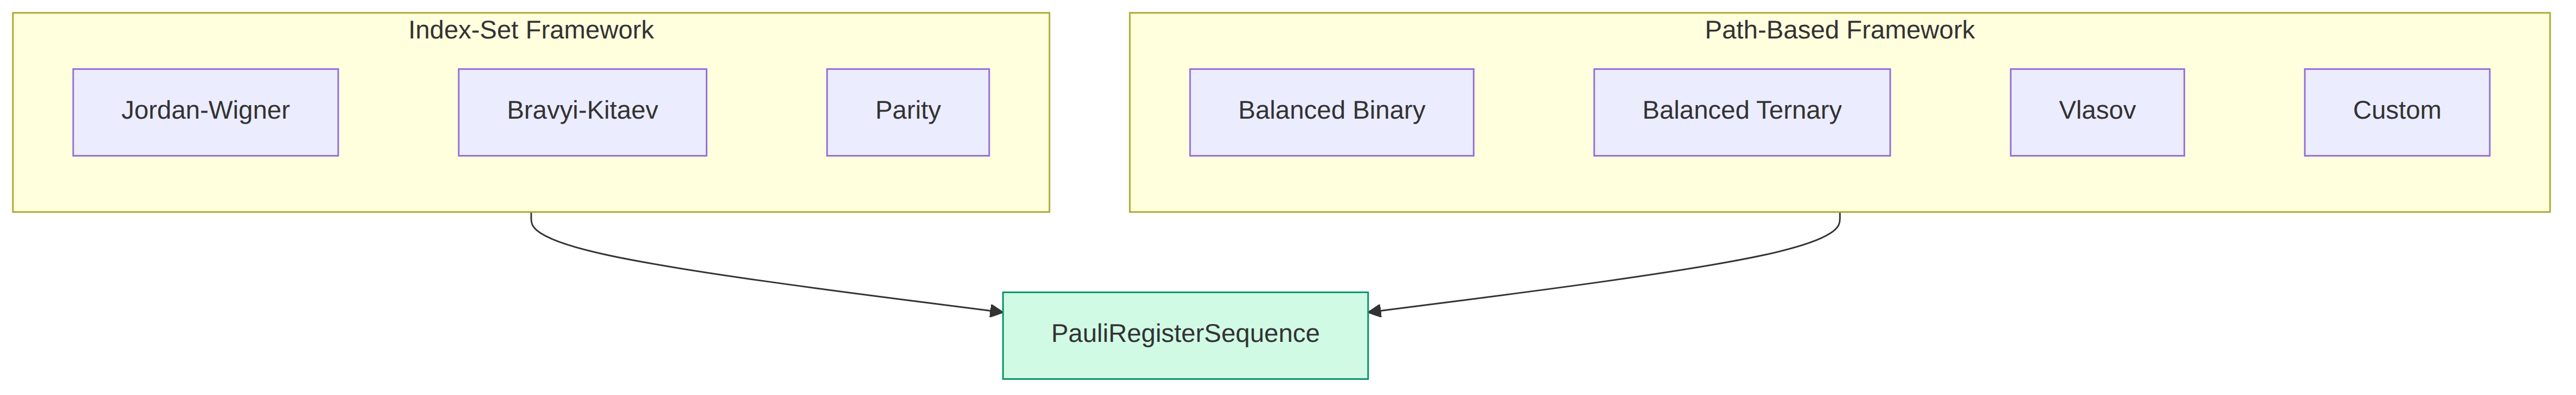
\includegraphics[keepaspectratio]{diagram-09.png}}

\textbf{Index-set framework} (MajoranaEncoding.fs): An encoding is
defined by three set-valued functions --- Update(\(j\)), Parity(\(j\)),
and Occupation(\(j\)). JW, BK, and Parity are each defined in 3--5 lines
of F\#.

\textbf{Path-based framework} (TreeEncoding.fs): An encoding is derived
from a labelled rooted tree. Any tree topology works --- strictly more
general than the index-set framework.

\textbf{Fenwick-specific} (BravyiKitaev.fs): BK uses hand-derived
bit-manipulation formulas specific to the Fenwick tree. Faster than
generic tree traversal, same result.

\begin{quote}
\textbf{Design note:} The index-set framework was introduced by Seeley,
Richard, and Love (2012) as a unifying abstraction. Our investigation
showed that it produces correct encodings \emph{only} for star-shaped
(depth-1) trees --- a previously undocumented constraint. The path-based
framework (Jiang et al., 2020) removes this restriction. FockMap
provides both because the index-set framework is simpler and faster when
it applies.
\end{quote}

\subsection{Two ternary trees: why tree shape
matters}\label{two-ternary-trees-why-tree-shape-matters}

The path-based framework's generality has a concrete payoff: FockMap
ships \emph{two} ternary tree encodings that achieve the same optimal
\(O(\log_3 n)\) worst-case Pauli weight but use different tree shapes
--- the balanced ternary tree (Jiang et al., 2020) and the Vlasov tree
(Vlasov, arXiv:1904.09912). Both preserve the CAR, both produce the same
eigenvalues, but they assign qubits to tree nodes differently.

How does one go from a tree shape to a working encoding? That's the
subject of the next chapter, where we'll build the Vlasov tree step by
step --- define the tree, plug it into the framework, and verify that it
works.

\begin{center}\rule{0.5\linewidth}{0.5pt}\end{center}

\section{Defining Custom Encodings}\label{defining-custom-encodings}

FockMap supports two routes for custom encodings beyond the six built-in
options:

\textbf{Index-set route.} Define three set-valued functions --- Update,
Parity, Occupation --- and pass them as an \texttt{EncodingScheme}. This
works for star-shaped trees (JW, Parity) and is the simplest path.

\textbf{Tree-based route.} Define a tree shape and plug it into the
path-based framework. This is strictly more general and is the subject
of the next chapter, where we build the Vlasov tree from scratch.

\begin{quote}
\textbf{Warning:} Not every custom scheme produces a valid encoding.
Always verify the CAR before trusting results --- Chapter 8 shows how.
\end{quote}

\begin{center}\rule{0.5\linewidth}{0.5pt}\end{center}

\section{A Decision Framework}\label{a-decision-framework}

\begin{longtable}[]{@{}
  >{\raggedright\arraybackslash}p{(\linewidth - 4\tabcolsep) * \real{0.3333}}
  >{\raggedright\arraybackslash}p{(\linewidth - 4\tabcolsep) * \real{0.3333}}
  >{\raggedright\arraybackslash}p{(\linewidth - 4\tabcolsep) * \real{0.3333}}@{}}
\toprule\noalign{}
\begin{minipage}[b]{\linewidth}\raggedright
Situation
\end{minipage} & \begin{minipage}[b]{\linewidth}\raggedright
Recommended encoding
\end{minipage} & \begin{minipage}[b]{\linewidth}\raggedright
Reasoning
\end{minipage} \\
\midrule\noalign{}
\endhead
\bottomrule\noalign{}
\endlastfoot
Learning / prototyping & Jordan--Wigner & Simplest to understand and
debug \\
Small system (\(n \leq 16\)) & Jordan--Wigner & Weight overhead is
manageable \\
1D chain / local interactions & Jordan--Wigner & Adjacent-orbital terms
have short Z-chains \\
General-purpose (\(n \leq 100\)) & Bravyi--Kitaev & \(O(\log_2 n)\)
weight, well-studied \\
Minimum circuit depth & Ternary Tree or Vlasov Tree & \(O(\log_3 n)\)
--- best known asymptotic scaling \\
Exploring custom topologies & Path-based & Arbitrary tree shapes
supported \\
Comparing ternary tree variants & Vlasov Tree & Same scaling, different
qubit assignment \\
Comparing multiple encodings & All six & FockMap's interchangeable
interface makes this trivial \\
\end{longtable}

\begin{center}\rule{0.5\linewidth}{0.5pt}\end{center}

\section{Key Takeaways}\label{key-takeaways-6}

\begin{itemize}
\tightlist
\item
  JW's \(O(n)\) Pauli weight motivates the search for alternative
  encodings.
\item
  All valid encodings produce Hamiltonians with the \textbf{same
  eigenvalues} --- this follows from CAR preservation, not just
  empirical observation.
\item
  For H₂ (4 qubits), the encodings produce identical Pauli strings. The
  differences emerge at larger \(n\).
\item
  The scaling advantage of tree-based encodings becomes dramatic above
  \textasciitilde16 spin-orbitals.
\item
  Defining a custom encoding is 3--5 lines of F\# --- but verify CAR
  before trusting it.
\end{itemize}

\section{Common Mistakes}\label{common-mistakes-6}

\begin{enumerate}
\def\labelenumi{\arabic{enumi}.}
\item
  \textbf{Assuming different Pauli strings mean different physics.} They
  don't --- if the CAR is preserved, eigenvalues are preserved.
  Different strings, same physics.
\item
  \textbf{Choosing an encoding by term count.} All encodings produce the
  same number of Hamiltonian terms. The difference is Pauli
  \emph{weight} per term, which determines CNOT count.
\item
  \textbf{Using a custom encoding without verifying CAR.} An encoding
  that violates anti-commutation will produce plausible but wrong
  Hamiltonians. Always test.
\end{enumerate}

\section{Exercises}\label{exercises-6}

\begin{enumerate}
\def\labelenumi{\arabic{enumi}.}
\item
  \textbf{Weight table.} Run the scaling comparison for \(n = 64\) and
  \(n = 128\). At what point does the ternary tree's maximum weight
  exceed 10?
\item
  \textbf{CAR verification.} Define a custom encoding and use FockMap's
  test infrastructure to check whether it satisfies anti-commutation.
  What happens if it doesn't?
\item
  \textbf{Encoding comparison for H₂O.} Build the H₂O/STO-3G Hamiltonian
  (12 active spin-orbitals, frozen core) with all six encodings. Compare
  maximum and average Pauli weight.
\end{enumerate}

\section{Further Reading}\label{further-reading-6}

\begin{itemize}
\tightlist
\item
  Seeley, J. T., Richard, M. J., and Love, P. J. ``The Bravyi--Kitaev
  transformation for quantum computation of electronic structure.''
  \emph{J. Chem. Phys.} 137, 224109 (2012). The index-set framework.
\item
  Jiang, Z. et al.~``Optimal fermion-to-qubit mapping via ternary
  trees.'' \emph{PRX Quantum} 1, 010306 (2020). The path-based ternary
  tree encoding.
\item
  Vlasov, A. Yu. ``Clifford algebras, Spin groups and qubit trees.''
  arXiv:1904.09912 (2019/2022). The complete ternary tree encoding via
  Clifford algebra.
\item
  Tranter, A. et al.~``The Bravyi--Kitaev transformation: Properties and
  applications.'' \emph{Int. J. Quantum Chem.} 115, 1431 (2015).
  Practical JW vs BK comparison.
\end{itemize}

\begin{center}\rule{0.5\linewidth}{0.5pt}\end{center}

\chapter{Chapter 8: Building a Tree
Encoding}\label{chapter-8-building-a-tree-encoding}

\emph{Chapter 7 gave us six encodings. This chapter shows how we got the
sixth --- by building it from scratch.}

\section{In This Chapter}\label{in-this-chapter-7}

\begin{itemize}
\tightlist
\item
  \textbf{What you'll learn:} How the path-based tree framework turns a
  tree shape into a valid fermion-to-qubit encoding, how to define the
  Vlasov tree in a few lines of code, and how to verify that a new
  encoding preserves the canonical anti-commutation relations (CAR).
\item
  \textbf{Why this matters:} Understanding the framework well enough to
  build your own encoding means you're not limited to the built-in
  options. And the verification skills you'll develop here --- checking
  CAR, comparing eigenvalues --- are the same skills you'll need for
  every pipeline you build.
\item
  \textbf{Prerequisites:} Chapter 7 (you know the six encodings, the two
  frameworks, and the CAR theorem).
\end{itemize}

\begin{quote}
\textbf{Scope note:} This chapter covers the tree-based (path-based)
route to custom encodings. Chapter 7 briefly introduced the index-set
route, which works for star-shaped trees. The tree-based route is
strictly more general.
\end{quote}

\begin{center}\rule{0.5\linewidth}{0.5pt}\end{center}

\section{The Goal}\label{the-goal}

In Chapter 7, we listed six encodings and noted that FockMap ships
\emph{two} ternary tree encodings: the balanced ternary tree (Jiang et
al., 2020) and the Vlasov tree (Vlasov, arXiv:1904.09912). Both achieve
\(O(\log_3 n)\) worst-case Pauli weight, but they assign qubits to tree
nodes differently.

How did the Vlasov tree get into FockMap? Someone had to define the tree
shape, plug it into the path-based framework, and verify that the result
was a valid encoding. In this chapter, we'll walk through exactly that
process --- and by the end, you'll be able to do the same for any tree
shape you can imagine.

\begin{quote}
I am grateful to Dr Robin Kothari and Dr Stephen Jordan for bringing
Vlasov's construction to my attention. Their suggestion led directly to
the implementation we'll develop here.
\end{quote}

\begin{center}\rule{0.5\linewidth}{0.5pt}\end{center}

\section{Step 1: Define the Tree
Shape}\label{step-1-define-the-tree-shape}

The Vlasov tree is a \textbf{complete ternary tree} with
\textbf{breadth-first (level-order) indexing}. Node 0 is the root. The
children of node \(j\) are \(3j+1\), \(3j+2\), and \(3j+3\) --- the same
formula used to index a heap in computer science.

For \(n = 9\) modes:

\pandocbounded{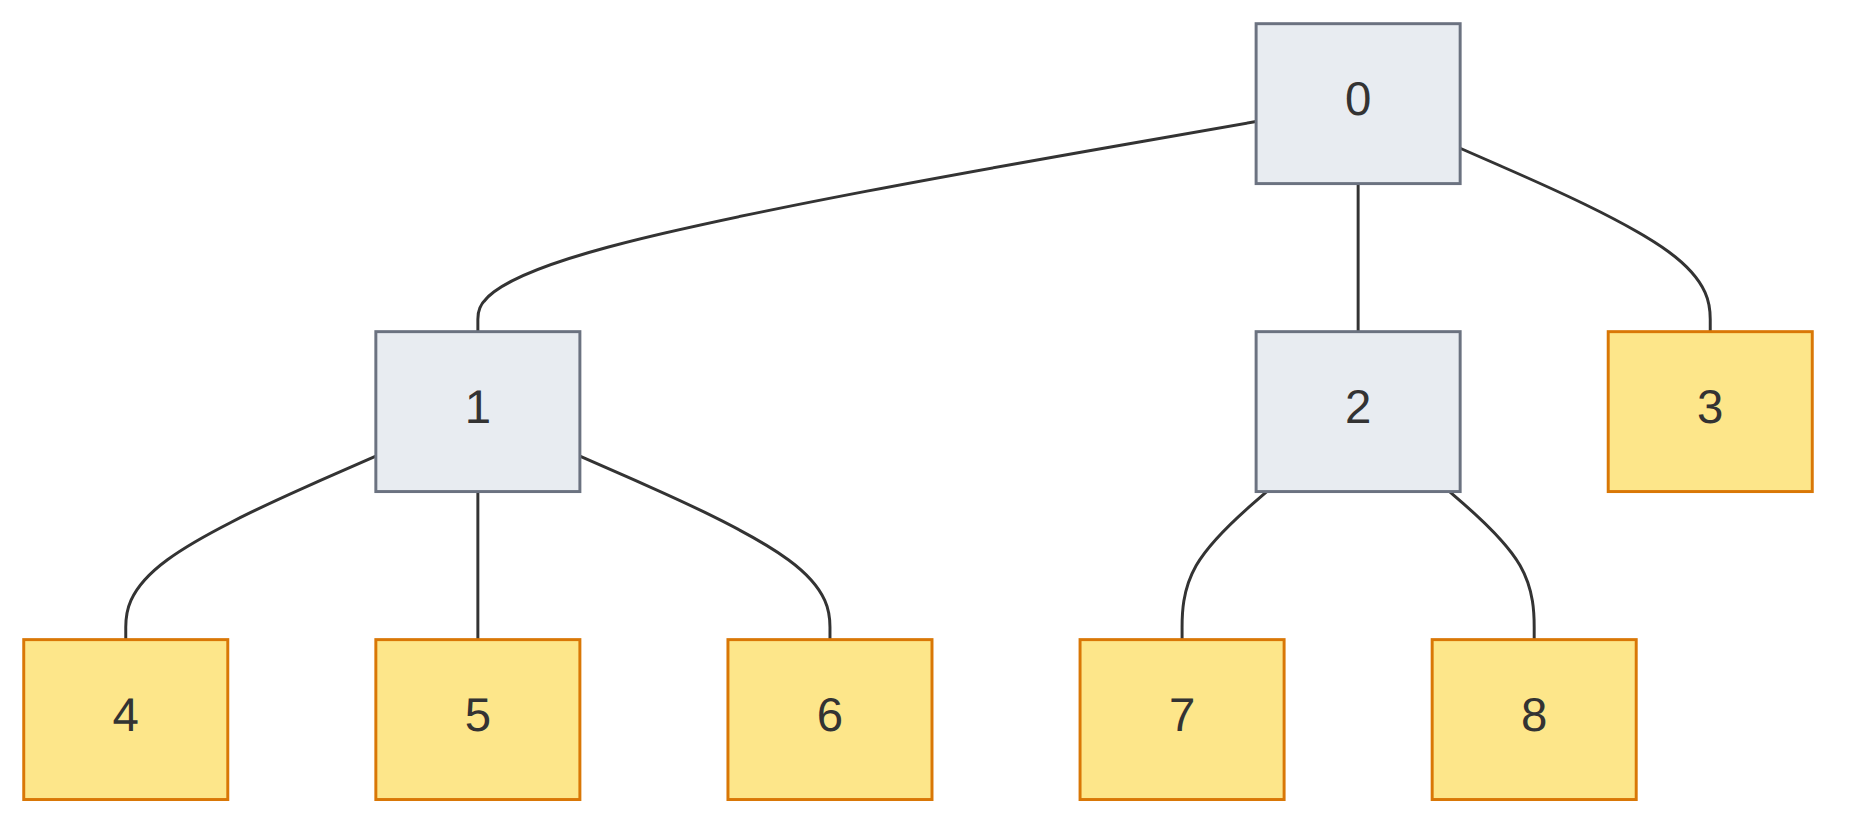
\includegraphics[keepaspectratio]{diagram-10.png}}

Node 0 has children 1, 2, 3. Node 1 has children 4, 5, 6. Node 2 has
children 7, 8. Node 3 is a leaf --- its would-be children (9, 10, 11)
all fall outside \(n = 9\).

Compare this with the balanced ternary tree, which uses a recursive
midpoint partition: for 9 modes, it puts modes 0--2 in the left subtree,
modes 3--5 in the middle, and modes 6--8 on the right. The tree has the
same branching factor but a completely different assignment of mode
indices to tree positions.

\subsection{The code}\label{the-code}

In FockMap, a tree is built from \texttt{TreeNode} records:

\begin{Shaded}
\begin{Highlighting}[]
\KeywordTok{let} \KeywordTok{rec}\NormalTok{ buildNode j parent =}
    \KeywordTok{let}\NormalTok{ childIndices =}
        \OperatorTok{[}\DecValTok{3}\NormalTok{*j+}\DecValTok{1}\NormalTok{; }\DecValTok{3}\NormalTok{*j+}\DecValTok{2}\NormalTok{; }\DecValTok{3}\NormalTok{*j+}\DecValTok{3}\OperatorTok{]}\NormalTok{ |\textgreater{} List}\KeywordTok{.}\NormalTok{filter }\OperatorTok{(}\KeywordTok{fun}\NormalTok{ c {-}\textgreater{} c \textless{} n}\OperatorTok{)}
    \KeywordTok{let}\NormalTok{ children =}
\NormalTok{        childIndices |\textgreater{} List}\KeywordTok{.}\NormalTok{map }\OperatorTok{(}\KeywordTok{fun}\NormalTok{ c {-}\textgreater{} buildNode c }\OperatorTok{(}\NormalTok{Some j}\OperatorTok{))}
\NormalTok{    mkNode j children parent}

\KeywordTok{let}\NormalTok{ tree = mkTree }\OperatorTok{(}\NormalTok{buildNode }\DecValTok{0}\NormalTok{ None}\OperatorTok{)}\NormalTok{ n}
\end{Highlighting}
\end{Shaded}

Three lines of logic --- the rest is plumbing. The key is the child
formula: \texttt{3*j+1}, \texttt{3*j+2}, \texttt{3*j+3}. Everything else
follows from this.

\begin{center}\rule{0.5\linewidth}{0.5pt}\end{center}

\section{Step 2: Plug It Into the
Framework}\label{step-2-plug-it-into-the-framework}

The path-based framework takes an \texttt{EncodingTree} and produces
Pauli strings. Internally, it traces the path from the root to each
leaf, collecting Pauli labels (X, Y, Z) on each edge. The tree shape
determines the paths; the paths determine the Pauli strings; the Pauli
strings determine the encoding.

FockMap wraps this in a one-line convenience function:

\begin{Shaded}
\begin{Highlighting}[]
\KeywordTok{let}\NormalTok{ vlasovTreeTerms }\OperatorTok{(}\NormalTok{op : LadderOperatorUnit}\OperatorTok{)} \OperatorTok{(}\NormalTok{j : }\DataTypeTok{uint32}\OperatorTok{)} \OperatorTok{(}\NormalTok{n : }\DataTypeTok{uint32}\OperatorTok{)}\NormalTok{ =}
    \KeywordTok{let}\NormalTok{ tree = vlasovTree }\OperatorTok{(}\DataTypeTok{int}\NormalTok{ n}\OperatorTok{)}
\NormalTok{    encodeWithTernaryTree tree op j n}
\end{Highlighting}
\end{Shaded}

That's the complete encoding --- define the tree, call the generic
encoder. The \texttt{encodeWithTernaryTree} function handles edge
labelling, path traversal, Majorana construction, and phase tracking.
You provide only the shape.

\begin{center}\rule{0.5\linewidth}{0.5pt}\end{center}

\section{Step 3: Compare the Tree
Shapes}\label{step-3-compare-the-tree-shapes}

Before we verify correctness, let's see what the two ternary trees
actually look like for \(n = 8\):

\begin{Shaded}
\begin{Highlighting}[]
\KeywordTok{let}\NormalTok{ vlTree = vlasovTree }\DecValTok{8}
\KeywordTok{let}\NormalTok{ btTree = balancedTernaryTree }\DecValTok{8}
\end{Highlighting}
\end{Shaded}

\textbf{Vlasov tree} (\(n = 8\), level-order):

\pandocbounded{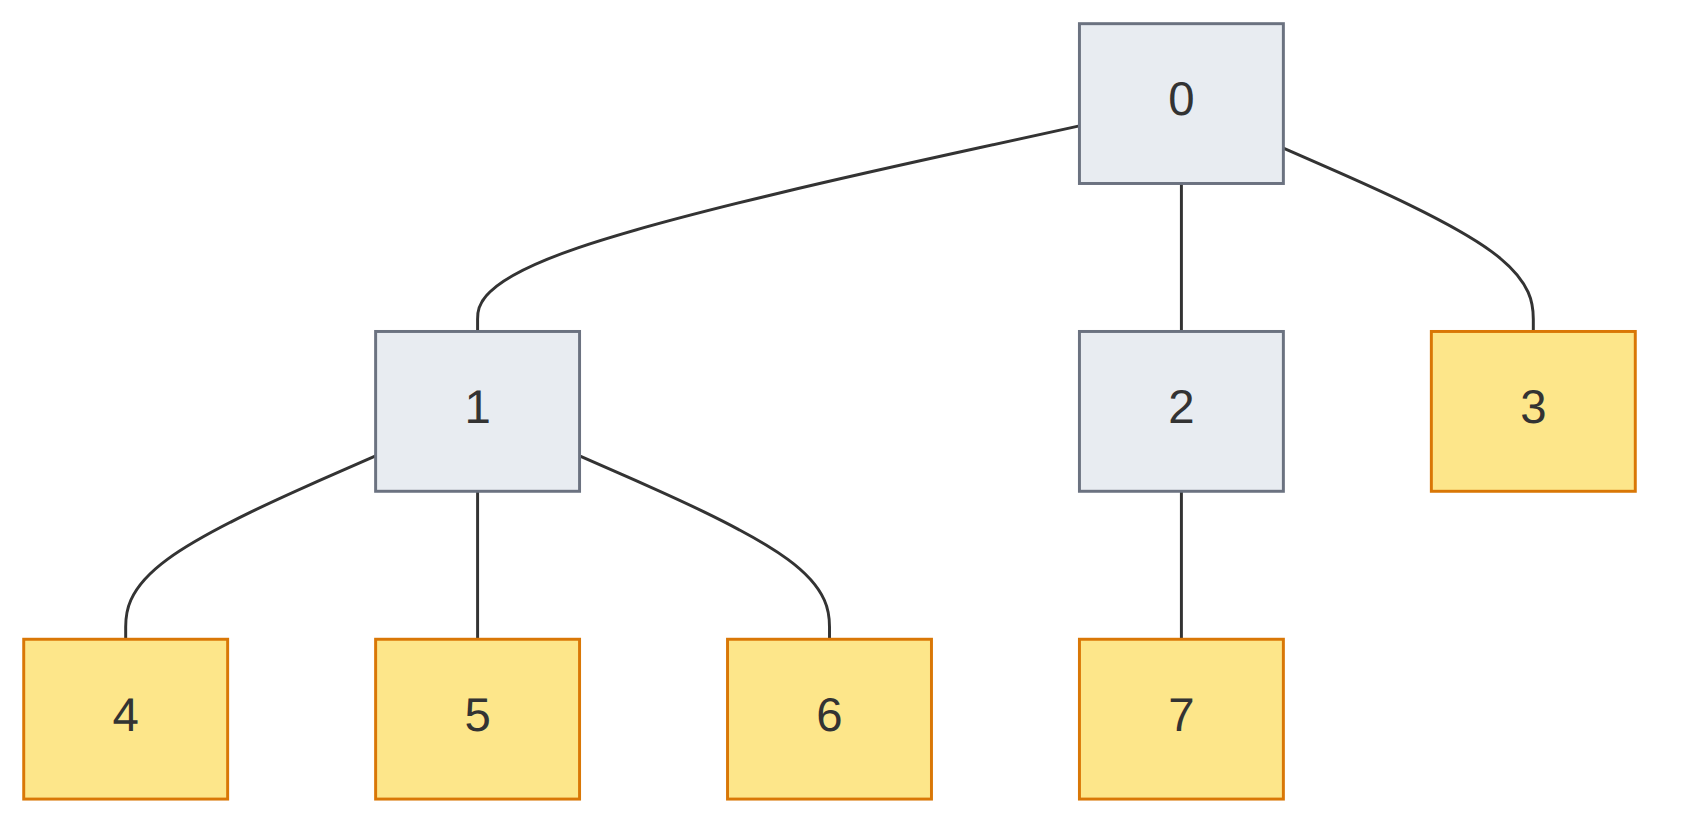
\includegraphics[keepaspectratio]{diagram-11.png}}

\textbf{Balanced ternary tree} (\(n = 8\), midpoint-split, root = mode
4):

\pandocbounded{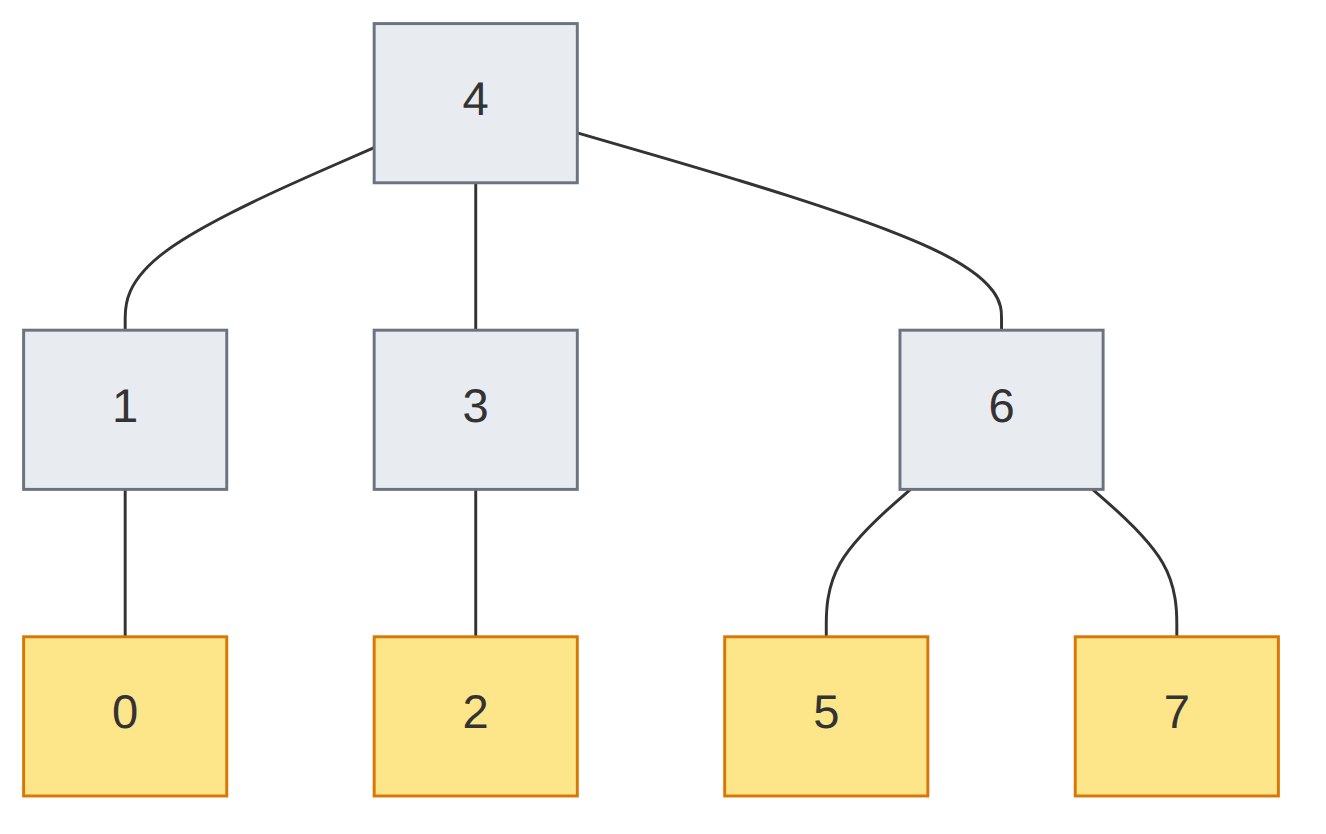
\includegraphics[keepaspectratio]{diagram-12.png}}

Different roots, different parent--child relationships, different path
lengths for some modes. Yet both produce valid encodings with the same
asymptotic weight.

\subsection{What do the Pauli strings look
like?}\label{what-do-the-pauli-strings-look-like}

Encode the creation operator \(a_3^\dagger\) on 8 modes with both trees:

\begin{Shaded}
\begin{Highlighting}[]
\KeywordTok{let}\NormalTok{ btTerms = ternaryTreeTerms Raise }\DecValTok{3}\NormalTok{u }\DecValTok{8}\NormalTok{u}
\KeywordTok{let}\NormalTok{ vlTerms = vlasovTreeTerms Raise }\DecValTok{3}\NormalTok{u }\DecValTok{8}\NormalTok{u}
\end{Highlighting}
\end{Shaded}

The Pauli strings are \emph{different} --- different signatures,
different coefficients. But both satisfy the CAR, and both produce
Hamiltonians with the same eigenvalues.

\begin{center}\rule{0.5\linewidth}{0.5pt}\end{center}

\section{Step 4: Verify Correctness}\label{step-4-verify-correctness}

There are two levels of verification, and you should do both.

\subsection{Level 1: Check the CAR}\label{level-1-check-the-car}

A valid encoding must satisfy the canonical anti-commutation relations:

\[\{a_i^\dagger, a_j\} = \delta_{ij} \cdot I, \qquad \{a_i^\dagger, a_j^\dagger\} = 0, \qquad \{a_i, a_j\} = 0\]

FockMap's test infrastructure checks these symbolically --- multiplying
encoded Pauli strings and verifying the algebra. If the CAR check
passes, the encoding is algebraically valid: the encoded Hamiltonian is
guaranteed to have the correct spectrum.

\begin{Shaded}
\begin{Highlighting}[]
\NormalTok{//}\CommentTok{ For each pair (i, j), verify anti{-}commutation}
\KeywordTok{for}\NormalTok{ i }\KeywordTok{in} \DecValTok{0}\NormalTok{u .. n}\DecValTok{{-}1}\NormalTok{u }\KeywordTok{do}
    \KeywordTok{for}\NormalTok{ j }\KeywordTok{in} \DecValTok{0}\NormalTok{u .. n}\DecValTok{{-}1}\NormalTok{u }\KeywordTok{do}
        \KeywordTok{let}\NormalTok{ ai\_dag = vlasovTreeTerms Raise i n}
        \KeywordTok{let}\NormalTok{ aj     = vlasovTreeTerms Lower j n}
\NormalTok{        //}\CommentTok{ Compute \{a†\_i, a\_j\} and check = delta\_ij * I}
\end{Highlighting}
\end{Shaded}

This is what FockMap's property tests do for all six encodings at every
system size from 1 to 32.

\subsection{Level 2: Compare
eigenvalues}\label{level-2-compare-eigenvalues}

Build the H₂ Hamiltonian with the new encoding and compare eigenvalues
against a known-good encoding:

\begin{Shaded}
\begin{Highlighting}[]
\KeywordTok{let}\NormalTok{ vlHam = computeHamiltonianWith vlasovTreeTerms factory }\DecValTok{4}\NormalTok{u}
\KeywordTok{let}\NormalTok{ jwHam = computeHamiltonianWith jordanWignerTerms factory }\DecValTok{4}\NormalTok{u}
\NormalTok{//}\CommentTok{ Diagonalize both → eigenvalues must match to machine precision}
\end{Highlighting}
\end{Shaded}

The CAR check tells you the algebra is right. The eigenvalue comparison
tells you the full pipeline --- tree construction, path traversal,
Majorana assembly, Hamiltonian construction --- is correct end-to-end.

\begin{center}\rule{0.5\linewidth}{0.5pt}\end{center}

\section{The Weight Comparison}\label{the-weight-comparison}

Now that we trust the encoding, let's see how it compares:

\begin{longtable}[]{@{}ccccc@{}}
\toprule\noalign{}
Mode & JW & BK & Balanced Ternary & Vlasov \\
\midrule\noalign{}
\endhead
\bottomrule\noalign{}
\endlastfoot
0 & 1 & 1 & 3 & 3 \\
1 & 2 & 2 & 3 & 3 \\
2 & 3 & 2 & 3 & 3 \\
3 & 4 & 3 & 3 & 3 \\
4 & 5 & 3 & 3 & 3 \\
5 & 6 & 3 & 3 & 3 \\
6 & 7 & 3 & 3 & 3 \\
7 & 8 & 4 & 4 & 3 \\
\end{longtable}

For \(n = 8\), both ternary trees have maximum weight 3--4, while JW
reaches 8 and BK reaches 4. The ternary trees are consistently better
for the high-index modes where JW's Z-chains are longest.

The two ternary trees have \emph{slightly} different per-mode weights
--- because different tree shapes put different modes at different
depths --- but the same worst-case scaling. This is the point: the
\(O(\log_3 n)\) guarantee comes from the ternary branching factor, not
from the specific assignment of modes to nodes.

\begin{center}\rule{0.5\linewidth}{0.5pt}\end{center}

\section{The Recipe for Any Tree}\label{the-recipe-for-any-tree}

You've now seen the complete process. Here it is as a recipe:

\begin{enumerate}
\def\labelenumi{\arabic{enumi}.}
\item
  \textbf{Choose a tree shape.} Any rooted tree with at most 3 children
  per internal node works. The branching factor determines the Pauli
  weight scaling.
\item
  \textbf{Implement the tree.} Use \texttt{mkNode} and \texttt{mkTree}
  to build the \texttt{EncodingTree}. The only creative part is the
  child-assignment rule.
\item
  \textbf{Call \texttt{encodeWithTernaryTree}.} The framework handles
  edge labelling, path traversal, and Majorana construction.
\item
  \textbf{Verify CAR.} Run the anti-commutation check for all pairs
  \((i, j)\) at several system sizes. If it fails, your tree
  construction has a bug.
\item
  \textbf{Compare eigenvalues.} Build a Hamiltonian and compare against
  a known encoding. If eigenvalues match to machine precision, the full
  pipeline is correct.
\end{enumerate}

The entire Vlasov encoding --- from Vlasov's paper to a verified FockMap
function --- took 6 lines of tree construction, 3 lines of wrapper, and
a test suite that matches the property tests used for every other
encoding.

\begin{center}\rule{0.5\linewidth}{0.5pt}\end{center}

\section{Key Takeaways}\label{key-takeaways-7}

\begin{itemize}
\tightlist
\item
  The path-based framework turns \textbf{any tree shape} into a valid
  encoding. You provide the shape; the framework provides the algebra.
\item
  The Vlasov tree uses level-order indexing (\(3j+1\), \(3j+2\),
  \(3j+3\)) --- a different qubit assignment than the balanced ternary
  tree, but the same asymptotic weight.
\item
  \textbf{Verification is non-negotiable.} A tree that looks reasonable
  can still violate the CAR. Always check anti-commutation before
  trusting results.
\item
  Two verification levels: symbolic CAR check (algebraic guarantee) and
  eigenvalue comparison (end-to-end pipeline check).
\item
  Building a new encoding is \textbf{fast} --- a few lines of tree
  construction, plus the validation effort. The path-based framework
  removes all the hard algebra.
\end{itemize}

\section{Exercises}\label{exercises-7}

\begin{enumerate}
\def\labelenumi{\arabic{enumi}.}
\item
  \textbf{A lopsided ternary tree.} Build a ternary tree for \(n = 9\)
  where each node has exactly one child --- node 0's only child is node
  1, node 1's only child is node 2, and so on. What is the worst-case
  Pauli weight? How does it compare to JW? (You've just rediscovered why
  JW has \(O(n)\) scaling --- it \emph{is} a depth-\(n\) chain tree.)
\item
  \textbf{Asymmetric tree.} Build a ternary tree where the left subtree
  has depth 2 and the right subtree has depth 4. How does the per-mode
  weight distribution differ from a balanced tree? Is the worst case
  better or worse?
\item
  \textbf{Vlasov vs balanced at scale.} Compare the Vlasov and balanced
  ternary trees at \(n = 27\) (a perfect power of 3). Do the per-mode
  weights differ? What about \(n = 30\) (not a perfect power)?
\item
  \textbf{Try the lab.} Run the
  \href{../labs/10-vlasov-tree.html}{Vlasov tree lab} to see the tree
  shapes and per-mode weight comparisons in action.
\end{enumerate}

\section{Further Reading}\label{further-reading-7}

\begin{itemize}
\tightlist
\item
  Vlasov, A. Yu. ``Clifford algebras, Spin groups and qubit trees.''
  \emph{Quanta} 11, 97--114 (2022). arXiv:1904.09912 (2019). The
  original construction.
\item
  Jiang, Z. et al.~``Optimal fermion-to-qubit mapping via ternary
  trees.'' \emph{PRX Quantum} 1, 010306 (2020). The balanced ternary
  tree and path-based framework.
\end{itemize}

\begin{center}\rule{0.5\linewidth}{0.5pt}\end{center}

\chapter{Chapter 9: Checking Our
Answer}\label{chapter-9-checking-our-answer}

\emph{We have fifteen Pauli strings and fifteen coefficients. How do we
know they're right? Chapter 8 showed how to verify an encoding
algebraically --- checking that the CAR hold at the Pauli string level.
This chapter adds the second, independent check: compute the eigenvalues
and compare with a known reference.}

\section{In This Chapter}\label{in-this-chapter-8}

\begin{itemize}
\tightlist
\item
  \textbf{What you'll learn:} How to verify an encoded Hamiltonian by
  exact diagonalization, how to interpret the eigenspectrum by
  particle-number sector, and how to confirm that all six encodings
  produce the same physics.
\item
  \textbf{Why this matters:} Algebraic validation (Chapter 8) guarantees
  the encoding is correct in isolation. But the full pipeline ---
  integrals, coefficient assembly, like-term combination --- has many
  other places where bugs can hide. Eigenvalue comparison catches them
  all. If you skip this step, you will eventually publish a wrong
  number.
\item
  \textbf{Prerequisites:} Chapters 1--8 (you have the 15-term
  Hamiltonian from all six encodings and understand both algebraic and
  numerical verification).
\end{itemize}

\begin{center}\rule{0.5\linewidth}{0.5pt}\end{center}

\section{The Verification Problem}\label{the-verification-problem}

Here is a sobering fact about fermion-to-qubit encoding: \textbf{most
bugs produce plausible output.}

A wrong-convention Hamiltonian (Chapter 2, Error \#1) has 15 terms with
real coefficients and the right Pauli symmetries. A missing cross-spin
block (Chapter 3, Mistake \#1) has fewer exchange terms but still looks
like a valid Hamiltonian. A reversed operator ordering (Chapter 6,
Mistake \#2) flips some signs but leaves the structure intact.

None of these errors will crash your code. All of them will give wrong
eigenvalues. The only way to catch them is to compute those eigenvalues
and compare with a known reference.

For H₂ in STO-3G, we have exact classical reference values. For larger
molecules, we can still cross-check between encodings --- if all six
give the same spectrum, we can be confident in the pipeline (though not
in the integrals, which must be checked separately).

\begin{center}\rule{0.5\linewidth}{0.5pt}\end{center}

\section{From Pauli Sum to Matrix}\label{from-pauli-sum-to-matrix}

This is the one place where we leave the symbolic world and build a
matrix. We do this \emph{only} for verification --- the actual quantum
simulation never needs a matrix.

Each single-qubit Pauli operator has a \(2 \times 2\) matrix:

\[I = \begin{pmatrix}1&0\\0&1\end{pmatrix}, \quad X = \begin{pmatrix}0&1\\1&0\end{pmatrix}, \quad Y = \begin{pmatrix}0&-i\\i&0\end{pmatrix}, \quad Z = \begin{pmatrix}1&0\\0&-1\end{pmatrix}\]

A 4-qubit Pauli string like \(IIZZ\) is the tensor product
\(I \otimes I \otimes Z \otimes Z\) --- a \(16 \times 16\) matrix. The
full Hamiltonian matrix is the weighted sum:

\[H = \sum_{\alpha=1}^{15} c_\alpha \cdot (\text{tensor product of } \sigma_{\alpha,0} \otimes \sigma_{\alpha,1} \otimes \sigma_{\alpha,2} \otimes \sigma_{\alpha,3})\]

For 4 qubits, this is a \(16 \times 16\) Hermitian matrix. Diagonalizing
it gives 16 eigenvalues.

\begin{quote}
\textbf{Why 16 and not 6?} The 4-qubit Hilbert space has \(2^4 = 16\)
basis states, but H₂ has only 2 electrons --- so only 6 of those states
(\(\binom{4}{2} = 6\)) have the right particle number. The remaining 10
eigenvalues belong to the 0-electron, 1-electron, 3-electron, and
4-electron sectors. They are physically meaningful (they represent the
spectrum with different electron counts) but they are not the ground
state we are looking for.
\end{quote}

\begin{center}\rule{0.5\linewidth}{0.5pt}\end{center}

\section{The Eigenspectrum of H₂}\label{the-eigenspectrum-of-hux2082}

Diagonalizing the 15-term JW Hamiltonian gives eigenvalues grouped by
particle-number sector:

\begin{longtable}[]{@{}
  >{\centering\arraybackslash}p{(\linewidth - 4\tabcolsep) * \real{0.3571}}
  >{\centering\arraybackslash}p{(\linewidth - 4\tabcolsep) * \real{0.3571}}
  >{\raggedright\arraybackslash}p{(\linewidth - 4\tabcolsep) * \real{0.2857}}@{}}
\toprule\noalign{}
\begin{minipage}[b]{\linewidth}\centering
Sector (\(N_e\))
\end{minipage} & \begin{minipage}[b]{\linewidth}\centering
States
\end{minipage} & \begin{minipage}[b]{\linewidth}\raggedright
Eigenvalues \(E_\text{el}\) (Ha)
\end{minipage} \\
\midrule\noalign{}
\endhead
\bottomrule\noalign{}
\endlastfoot
0 & 1 & \(0\) \\
1 & 4 & \(-1.2563,\; -1.2563,\; -0.4719,\; -0.4719\) \\
\textbf{2} & \textbf{6} &
\(\mathbf{-1.8573},\; -1.3390,\; -0.9032,\; -0.9032,\; -0.6753,\; 0.0\) \\
3 & 4 & \(-1.7282,\; -1.7282,\; -0.9438,\; -0.9438\) \\
4 & 1 & \(-2.2001\) \\
\end{longtable}

The ground state of the physical 2-electron sector is
\(E_0^\text{el} = -1.8573\) Ha. Adding nuclear repulsion:

\[\boxed{E_0^\text{total} = E_0^\text{el} + V_{nn} = -1.8573 + 0.7151 = -1.1422 \text{ Ha}}\]

This is the \textbf{exact} ground-state energy of H₂ in the STO-3G basis
--- not an approximation, not a truncation, but the answer you'd get
from full configuration interaction (Full CI). A quantum computer
running VQE or QPE on this Hamiltonian should converge to this value.

\begin{center}\rule{0.5\linewidth}{0.5pt}\end{center}

\section{How Good Is This?}\label{how-good-is-this}

Let's put the number in context by comparing with simpler
approximations:

\begin{longtable}[]{@{}
  >{\raggedright\arraybackslash}p{(\linewidth - 6\tabcolsep) * \real{0.2222}}
  >{\centering\arraybackslash}p{(\linewidth - 6\tabcolsep) * \real{0.2778}}
  >{\centering\arraybackslash}p{(\linewidth - 6\tabcolsep) * \real{0.2778}}
  >{\raggedright\arraybackslash}p{(\linewidth - 6\tabcolsep) * \real{0.2222}}@{}}
\toprule\noalign{}
\begin{minipage}[b]{\linewidth}\raggedright
Method
\end{minipage} & \begin{minipage}[b]{\linewidth}\centering
\(E_\text{total}\) (Ha)
\end{minipage} & \begin{minipage}[b]{\linewidth}\centering
Error (kcal/mol)
\end{minipage} & \begin{minipage}[b]{\linewidth}\raggedright
What it captures
\end{minipage} \\
\midrule\noalign{}
\endhead
\bottomrule\noalign{}
\endlastfoot
Hartree--Fock & \(-1.1168\) & \(15.9\) & Mean-field (no correlation) \\
MP2 & \(-1.1381\) & \(2.6\) & Perturbative correlation \\
Full CI (= our result) & \(-1.1422\) & \(0\) & Exact (within basis) \\
Chemical accuracy target & --- & \(< 1.0\) & The goal for quantum
chemistry \\
\end{longtable}

The Hartree--Fock error of 15.9 kcal/mol is large --- it would
mispredict reaction rates by orders of magnitude. Our Full CI result
captures the entire correlation energy within the STO-3G basis. In the
language of Chapter 6, this 15.9 kcal/mol is exactly the energy
contribution of the off-diagonal terms in \(\text{Tr}(\rho H)\) --- the
coherences in the density matrix, generated by the 4 exchange Pauli
strings, that Hartree--Fock's diagonal \(\rho\) cannot capture.

Of course, STO-3G is a minimal basis --- the absolute energy is still
far from the true Born--Oppenheimer value. But within the model space
we've defined, our answer is exact.

\begin{quote}
\textbf{The point of quantum simulation is not to replace the basis set}
--- it's to solve the electronic problem \emph{exactly} within whatever
basis the user chooses, even for molecules where Full CI is classically
intractable. For H₂ in STO-3G (6 configurations), any laptop can do Full
CI. For a molecule with 50 electrons in 100 spin-orbitals
(\(\binom{100}{50} \approx 10^{29}\) configurations), only a quantum
computer can.
\end{quote}

\begin{center}\rule{0.5\linewidth}{0.5pt}\end{center}

\section{Cross-Encoding Verification}\label{cross-encoding-verification}

The most powerful check: build the Hamiltonian with all six encodings
and verify that they produce the \textbf{same eigenspectrum}.

\begin{Shaded}
\begin{Highlighting}[]
\KeywordTok{for} \OperatorTok{(}\NormalTok{name, encoder}\OperatorTok{)} \KeywordTok{in}\NormalTok{ encoders }\KeywordTok{do}
    \KeywordTok{let}\NormalTok{ ham = computeHamiltonianWith encoder h2Factory }\DecValTok{4}\NormalTok{u}
\NormalTok{    //}\CommentTok{ ... build 16×16 matrix, diagonalize ...}
\NormalTok{    printfn }\StringTok{"\%{-}25s  E₀ = \%.10f Ha"}\NormalTok{ name groundStateEnergy}
\end{Highlighting}
\end{Shaded}

\begin{longtable}[]{@{}lcc@{}}
\toprule\noalign{}
Encoding & \(E_0^\text{el}\) (Ha) & \(\lvert\Delta E\rvert\) from JW \\
\midrule\noalign{}
\endhead
\bottomrule\noalign{}
\endlastfoot
Jordan--Wigner & \(-1.8572750302\) & --- \\
Bravyi--Kitaev & \(-1.8572750302\) & \(< 10^{-15}\) \\
Parity & \(-1.8572750302\) & \(< 10^{-15}\) \\
Balanced Binary Tree & \(-1.8572750302\) & \(< 10^{-15}\) \\
Balanced Ternary Tree & \(-1.8572750302\) & \(< 10^{-15}\) \\
Vlasov Tree & \(-1.8572750302\) & \(< 10^{-15}\) \\
\end{longtable}

\textbf{Agreement to \(5 \times 10^{-16}\) Ha} --- the limit of 64-bit
floating-point precision. The eigenvalues are identical to machine
epsilon.

This is not a coincidence. It is a mathematical guarantee: every valid
encoding preserves the canonical anti-commutation relations, and
therefore preserves the operator algebra, and therefore preserves every
eigenvalue. FockMap's test suite verifies the anti-commutation relations
symbolically (no eigenvalues needed), but the eigenvalue comparison
provides an independent numerical cross-check.

\begin{center}\rule{0.5\linewidth}{0.5pt}\end{center}

\section{A Verification Checklist}\label{a-verification-checklist}

When building and verifying an encoded Hamiltonian, check these in
order:

\begin{longtable}[]{@{}
  >{\centering\arraybackslash}p{(\linewidth - 6\tabcolsep) * \real{0.2941}}
  >{\raggedright\arraybackslash}p{(\linewidth - 6\tabcolsep) * \real{0.2353}}
  >{\raggedright\arraybackslash}p{(\linewidth - 6\tabcolsep) * \real{0.2353}}
  >{\raggedright\arraybackslash}p{(\linewidth - 6\tabcolsep) * \real{0.2353}}@{}}
\toprule\noalign{}
\begin{minipage}[b]{\linewidth}\centering
\#
\end{minipage} & \begin{minipage}[b]{\linewidth}\raggedright
Check
\end{minipage} & \begin{minipage}[b]{\linewidth}\raggedright
How
\end{minipage} & \begin{minipage}[b]{\linewidth}\raggedright
What failure means
\end{minipage} \\
\midrule\noalign{}
\endhead
\bottomrule\noalign{}
\endlastfoot
1 & Term count & Count Pauli strings & Missing/extra integrals \\
2 & Identity coefficient & Read \(IIII\) coefficient & Wrong \(V_{nn}\)
or integral sum \\
3 & Diagonal symmetry & All Z-only terms come in pairs (\(IIIZ/IIZI\),
etc.) & Broken spin symmetry \\
4 & Exchange terms present & Look for XX/YY terms & Missing cross-spin
integrals \\
5 & Cross-encoding agreement & Build with 2+ encodings, compare spectra
& Encoding bug \\
6 & Known reference & Compare \(E_0\) against published value &
Convention error \\
\end{longtable}

If check 4 fails (no exchange terms), the most likely cause is the
cross-spin bug from Chapter 3. If check 5 fails (different eigenvalues
from different encodings), there is a bug in the encoding implementation
itself --- which, if you're using FockMap, should not happen.

\begin{center}\rule{0.5\linewidth}{0.5pt}\end{center}

\section{Encoding Stage Complete}\label{encoding-stage-complete}

With verification done, we have walked the complete path from molecule
to validated qubit Hamiltonian:

\pandocbounded{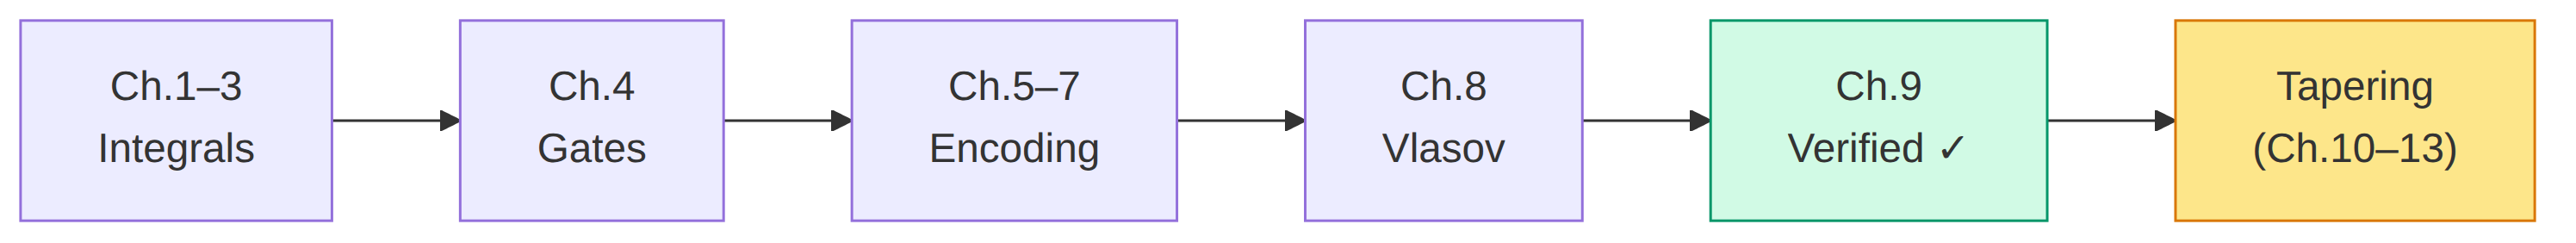
\includegraphics[keepaspectratio]{diagram-13.png}}

The Hamiltonian is correct. It is the exact qubit representation of H₂
in STO-3G for any of six encodings. It has 15 Pauli terms, its
ground-state energy is \(-1.1422\) Ha, and it captures all the electron
correlation that a quantum computer would extract.

But can we make it \emph{smaller}? Can we remove qubits without losing
physics? That's what tapering does --- and it's where we go next.

\begin{center}\rule{0.5\linewidth}{0.5pt}\end{center}

\section{Key Takeaways}\label{key-takeaways-8}

\begin{itemize}
\tightlist
\item
  Chapter 8 established \textbf{algebraic verification} (CAR checks).
  This chapter adds \textbf{numerical verification} (eigenvalue
  comparison). Both are necessary: algebraic checks validate the
  encoding; numerical checks validate the full pipeline.
\item
  The H₂/STO-3G ground-state energy is \(E_0 = -1.1422\) Ha (Full CI,
  exact within basis).
\item
  All six encodings produce eigenvalues that agree to
  \(< 5 \times 10^{-16}\) Ha --- machine precision.
\item
  Encoding bugs produce structurally plausible but numerically wrong
  Hamiltonians. Check eigenvalues early and often.
\item
  Matrix diagonalization is used \emph{only} for verification. The
  actual quantum simulation operates on the symbolic Pauli sum.
\end{itemize}

\section{Common Mistakes}\label{common-mistakes-7}

\begin{enumerate}
\def\labelenumi{\arabic{enumi}.}
\item
  \textbf{Verifying only the ground state.} Check the full spectrum (all
  particle-number sectors), not just \(E_0\). Some bugs preserve the
  ground state but corrupt excited states.
\item
  \textbf{Comparing absolute energies across basis sets.} STO-3G and
  cc-pVDZ give different energies for the same molecule. Only compare
  within the same basis.
\item
  \textbf{Skipping verification for ``trusted'' code.} Even well-tested
  libraries can produce wrong results if the integral input is wrong.
  Verify the first Hamiltonian you build for any new molecule.
\end{enumerate}

\section{Exercises}\label{exercises-8}

\begin{enumerate}
\def\labelenumi{\arabic{enumi}.}
\item
  \textbf{Sector analysis.} The 0-electron sector has eigenvalue 0. Why?
  (Hint: what does the Hamiltonian do to the vacuum state
  \(\lvert 0000\rangle\)?)
\item
  \textbf{Correlation energy.} Compute the Hartree--Fock energy of H₂ by
  hand: \(E_\text{HF} = h_{00} + h_{11} + [00\mid00] + V_{nn}\)
  (one-body energy for each spin-orbital in \(\sigma_g\), plus Coulomb
  repulsion, plus nuclear repulsion). Verify that
  \(E_\text{corr} = E_\text{FCI} - E_\text{HF} \approx -0.019\) Ha
  \(\approx -12\) kcal/mol. This is exactly the contribution of the
  off-diagonal exchange terms from Chapter 6.
\item
  \textbf{Cross-encoding lab.} Run the
  \href{../labs/03-compare-encodings.html}{Compare Encodings lab} and
  verify 6-encoding eigenvalue agreement for yourself.
\end{enumerate}

\section{Further Reading}\label{further-reading-8}

\begin{itemize}
\tightlist
\item
  Szabo, A. and Ostlund, N. S. \emph{Modern Quantum Chemistry.} §4.1
  gives the Full CI eigenvalues for H₂/STO-3G.
\item
  Helgaker, T., Jørgensen, P., and Olsen, J. \emph{Molecular
  Electronic-Structure Theory.} Chapter 12 covers Full CI theory and
  implementation.
\end{itemize}

\begin{center}\rule{0.5\linewidth}{0.5pt}\end{center}

\chapter{Chapter 10: Why Tapering?}\label{chapter-10-why-tapering}

\emph{The Hamiltonian is correct and verified. But it may be bigger than
it needs to be. This chapter shows why encoded Hamiltonians often
contain redundant qubits --- and how to detect them.}

\section{In This Chapter}\label{in-this-chapter-9}

\begin{itemize}
\tightlist
\item
  \textbf{What you'll learn:} How fermion-to-qubit encoding creates Z₂
  symmetries that allow safe qubit removal, and why this is one of the
  highest-leverage optimizations in the entire pipeline.
\item
  \textbf{Why this matters:} Removing even one qubit halves the Hilbert
  space. For near-term quantum hardware with limited qubit counts and
  high error rates, tapering can mean the difference between a feasible
  and an infeasible simulation.
\item
  \textbf{Prerequisites:} Chapters 1--9 (you have a verified qubit
  Hamiltonian and understand Pauli strings).
\end{itemize}

\begin{center}\rule{0.5\linewidth}{0.5pt}\end{center}

\section{The Observation}\label{the-observation}

Look again at the 15-term H₂ Hamiltonian from Chapter 6. Focus on the
Pauli operators at each qubit position:

\begin{longtable}[]{@{}
  >{\centering\arraybackslash}p{(\linewidth - 6\tabcolsep) * \real{0.2500}}
  >{\centering\arraybackslash}p{(\linewidth - 6\tabcolsep) * \real{0.2500}}
  >{\centering\arraybackslash}p{(\linewidth - 6\tabcolsep) * \real{0.2500}}
  >{\centering\arraybackslash}p{(\linewidth - 6\tabcolsep) * \real{0.2500}}@{}}
\toprule\noalign{}
\begin{minipage}[b]{\linewidth}\centering
Qubit 0
\end{minipage} & \begin{minipage}[b]{\linewidth}\centering
Qubit 1
\end{minipage} & \begin{minipage}[b]{\linewidth}\centering
Qubit 2
\end{minipage} & \begin{minipage}[b]{\linewidth}\centering
Qubit 3
\end{minipage} \\
\midrule\noalign{}
\endhead
\bottomrule\noalign{}
\endlastfoot
I, I, I, I, I, I, I, I, I, Z, Z, X, X, Y, Y & I, I, I, Z, Z, I, Z, Z, I,
I, Z, X, Y, X, Y & I, I, I, I, I, Z, I, Z, Z, Z, I, Y, Y, X, X & I, Z,
Z, I, I, Z, Z, I, Z, I, I, Y, X, Y, X \\
\end{longtable}

Every qubit has at least some terms with X or Y --- no qubit is purely
diagonal (I/Z only) across all 15 terms. So H₂ under JW has \textbf{no
diagonal Z₂ symmetries} at first glance.

But this is specific to H₂'s structure and the JW encoding. Many
molecular Hamiltonians --- especially larger ones --- \emph{do} have
qubits where every term is I or Z. And even when no single qubit is
diagonal, there may be \textbf{multi-qubit} Z₂ symmetries (like
\(Z_0 Z_1\)) that a Clifford rotation can exploit.

\subsection{Where diagonal symmetries come
from}\label{where-diagonal-symmetries-come-from}

Particle-number conservation is the most common source. In many
encodings, the total electron number operator
\(\hat{N} = \sum_j \hat{n}_j\) commutes with the Hamiltonian. Under JW,
\(\hat{N}\) maps to a sum of \(Z\) operators. If certain linear
combinations of these \(Z\) operators commute with every Hamiltonian
term, the corresponding qubits can be fixed and removed.

The Parity encoding makes this especially transparent: the last qubit
often stores the total parity of the electron number, which is conserved
--- making it immediately taperable.

\begin{center}\rule{0.5\linewidth}{0.5pt}\end{center}

\section{What Tapering Gains You}\label{what-tapering-gains-you}

The benefits are concrete and multiplicative:

\pandocbounded{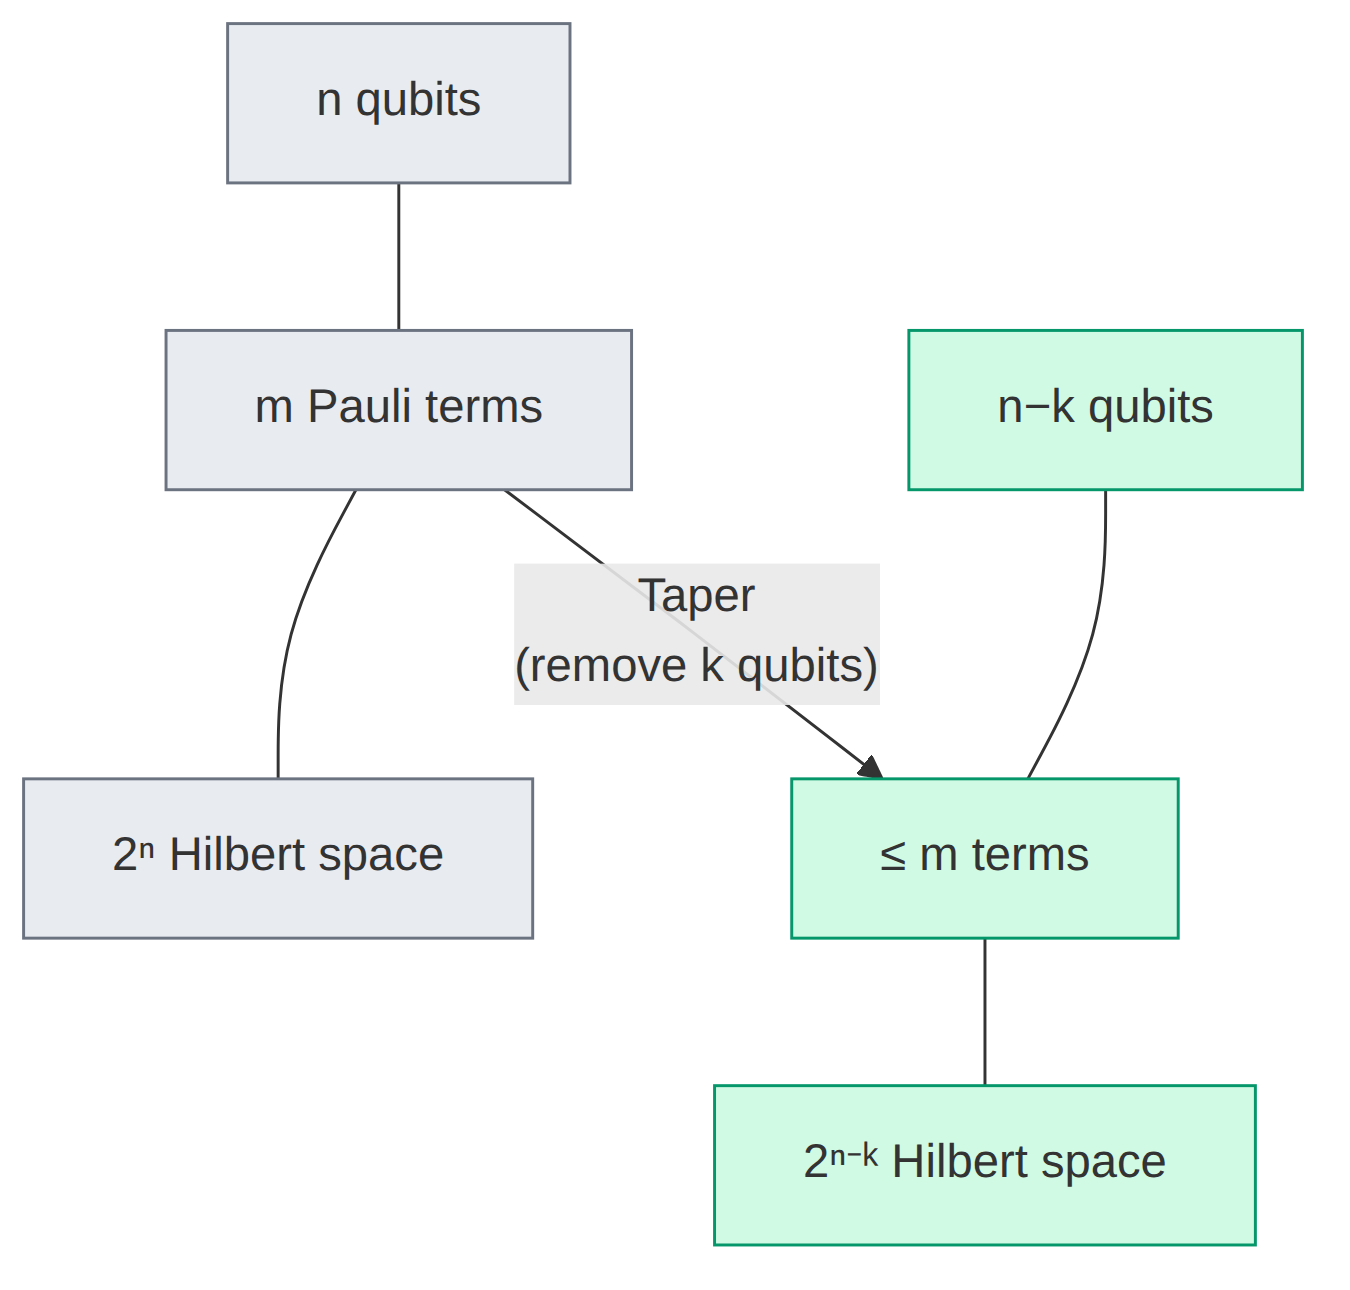
\includegraphics[keepaspectratio]{diagram-14.png}}

\begin{longtable}[]{@{}lcl@{}}
\toprule\noalign{}
What shrinks & Factor & Example (12 → 9 qubits) \\
\midrule\noalign{}
\endhead
\bottomrule\noalign{}
\endlastfoot
Qubit count & \(-k\) & 3 fewer physical qubits needed \\
Hilbert space & \(2^{-k}\) & \(4096 \to 512\) (8× smaller) \\
Circuit width & \(-k\) & 3 fewer wires in every gate layer \\
Pauli weight & often reduces & Shorter Z-chains after qubit removal \\
Term count & often reduces & Some terms collapse to identity \\
\end{longtable}

And these savings \textbf{compound} with encoding choice. A ternary-tree
encoding on a tapered Hamiltonian gets both the \(O(\log_3 n)\) weight
advantage \emph{and} the reduced qubit count.

\begin{center}\rule{0.5\linewidth}{0.5pt}\end{center}

\section{The Two Levels of Tapering}\label{the-two-levels-of-tapering}

FockMap implements two levels of increasing generality:

\subsection{Level 1: Diagonal Z₂}\label{level-1-diagonal-zux2082}

A qubit \(j\) is \emph{diagonally taperable} if every term in the
Hamiltonian has only I or Z at position \(j\) --- never X or Y. This
means qubit \(j\)'s value is determined by symmetry: it is always \(+1\)
or always \(-1\) in the sector we care about, and it never gets flipped
during the simulation. We can fix it to that value and remove it from
the problem entirely.

\textbf{How you detect it:} Look at each qubit position across all Pauli
terms. If you never see X or Y in that column, the qubit is taperable.
It's a simple scan --- FockMap checks this in one pass over the
Hamiltonian.

\subsection{Level 2: General Clifford}\label{level-2-general-clifford}

Sometimes no \emph{single} qubit is purely diagonal, but a
\emph{combination} of qubits is. For example, \(Z_0 Z_1\) might commute
with every Hamiltonian term even though \(Z_0\) alone does not. This
means the \emph{product} of qubits 0 and 1 is conserved, even though
neither one is individually.

In this case, we can apply a small rotation circuit (built from
Hadamard, S, and CNOT gates --- the same gates from Chapter 4) that
rearranges the Hamiltonian so that the conserved combination ends up on
a single qubit. After the rotation, that qubit is diagonally taperable,
and we remove it just like in Level 1.

\textbf{How you detect it:} FockMap searches for Pauli operators that
commute with every term in the Hamiltonian --- these are the symmetry
generators. The mathematical machinery behind this search involves
binary linear algebra, which we'll develop step by step in Chapter 12.

The important thing at this stage is the \emph{idea}: even when the
symmetry isn't visible on a single qubit, it may be hiding in a
combination of qubits, and a rotation can expose it.

We'll work through the diagonal case in Chapter 11, the Clifford
generalization in Chapter 12, and concrete benchmarks in Chapter 13.

\begin{center}\rule{0.5\linewidth}{0.5pt}\end{center}

\section{Why Tapering Is Free}\label{why-tapering-is-free}

It's worth emphasizing: tapering does not approximate. It does not
truncate. It does not discard information.

When we remove a tapered qubit, we are removing a degree of freedom
whose value was \emph{already determined} --- fixed by a conservation
law (like particle number or spin parity) that the Hamiltonian respects.
The qubit was never free to vary in the first place; it was constrained
by symmetry to a single eigenvalue in the sector we're studying.
Removing it simply acknowledges this constraint explicitly.

The eigenvalues of the tapered Hamiltonian are a \emph{subset} of the
eigenvalues of the original --- specifically, the eigenvalues in the
chosen symmetry sector. No eigenvalue is lost; we just stop tracking the
ones that belong to other sectors.

This is why we taper \emph{before} Trotterization, not after: the
circuit should operate on the physically relevant Hilbert space from the
start, not carry redundant qubits through every gate layer.

\begin{center}\rule{0.5\linewidth}{0.5pt}\end{center}

\section{Key Takeaways}\label{key-takeaways-9}

\begin{itemize}
\tightlist
\item
  Encoded Hamiltonians often have Z₂ symmetries --- qubits whose value
  is determined by conservation laws rather than dynamics.
\item
  Removing these qubits is free: it preserves the physics exactly while
  reducing every downstream cost.
\item
  Diagonal Z₂ symmetries (single-qubit Z generators) are the simplest
  case. General Z₂ symmetries require Clifford rotation.
\item
  Tapering compounds with encoding choice: taper first, then the
  encoding operates on a smaller system.
\end{itemize}

\section{Common Mistakes}\label{common-mistakes-8}

\begin{enumerate}
\def\labelenumi{\arabic{enumi}.}
\item
  \textbf{Assuming H₂ has taperable qubits under JW.} It doesn't --- the
  exchange terms (XXYY) put X/Y on every qubit. Tapering is most
  effective for larger molecules with more conservation laws.
\item
  \textbf{Confusing tapering with truncation.} Truncation (e.g.,
  active-space reduction) discards orbitals and loses information.
  Tapering removes redundant \emph{qubits} without losing any
  information --- the eigenvalues are exactly preserved.
\item
  \textbf{Tapering after circuit compilation.} Taper before
  Trotterization, not after. The circuit should be built on the smaller
  Hamiltonian.
\end{enumerate}

\section{Exercises}\label{exercises-9}

\begin{enumerate}
\def\labelenumi{\arabic{enumi}.}
\item
  \textbf{Conservation laws.} For a molecule with \(N\) electrons, what
  conservation laws might produce Z₂ symmetries? (Hint: total electron
  number, spin projection \(S_z\), point-group symmetry.)
\item
  \textbf{Parity encoding advantage.} Under the Parity encoding, the
  last qubit stores the total electron-number parity. Show that this
  qubit is always diagonally taperable for any Hamiltonian that
  conserves particle number.
\item
  \textbf{Scaling impact.} If tapering removes 3 qubits from a 14-qubit
  H₂O system, by what factor does the Hilbert space shrink? How many
  fewer CNOT gates does each Trotter step require (approximately)?
\end{enumerate}

\section{Further Reading}\label{further-reading-9}

\begin{itemize}
\tightlist
\item
  Bravyi, S., Gambetta, J. M., Mezzacapo, A., and Temme, K. ``Tapering
  off qubits to simulate fermionic Hamiltonians.'' arXiv:1701.08213
  (2017). The foundational paper on qubit tapering.
\end{itemize}

\begin{center}\rule{0.5\linewidth}{0.5pt}\end{center}

\chapter{Chapter 11: Diagonal Z₂
Symmetries}\label{chapter-11-diagonal-zux2082-symmetries}

\emph{The simplest form of tapering: find qubits that are always I or Z,
fix their eigenvalue, and remove them.}

\section{In This Chapter}\label{in-this-chapter-10}

\begin{itemize}
\tightlist
\item
  \textbf{What you'll learn:} The algorithm for detecting diagonal Z₂
  symmetries, how sector choice works, and how fixing a sector modifies
  each Pauli term.
\item
  \textbf{Why this matters:} Diagonal tapering is fast, easy to
  implement, and often removes 1--3 qubits from molecular Hamiltonians
  with zero information loss.
\item
  \textbf{Prerequisites:} Chapter 10 (you understand why tapering is
  valuable and what Z₂ symmetries are).
\end{itemize}

\begin{center}\rule{0.5\linewidth}{0.5pt}\end{center}

\section{The Detection Algorithm}\label{the-detection-algorithm}

Given a Hamiltonian \(\hat{H} = \sum_\alpha c_\alpha \sigma_\alpha\), we
say qubit \(j\) is \textbf{diagonal Z₂ symmetric} if:

\[\forall \alpha:\; \sigma_\alpha[j] \in \{I, Z\}\]

The algorithm is a single scan:

\pandocbounded{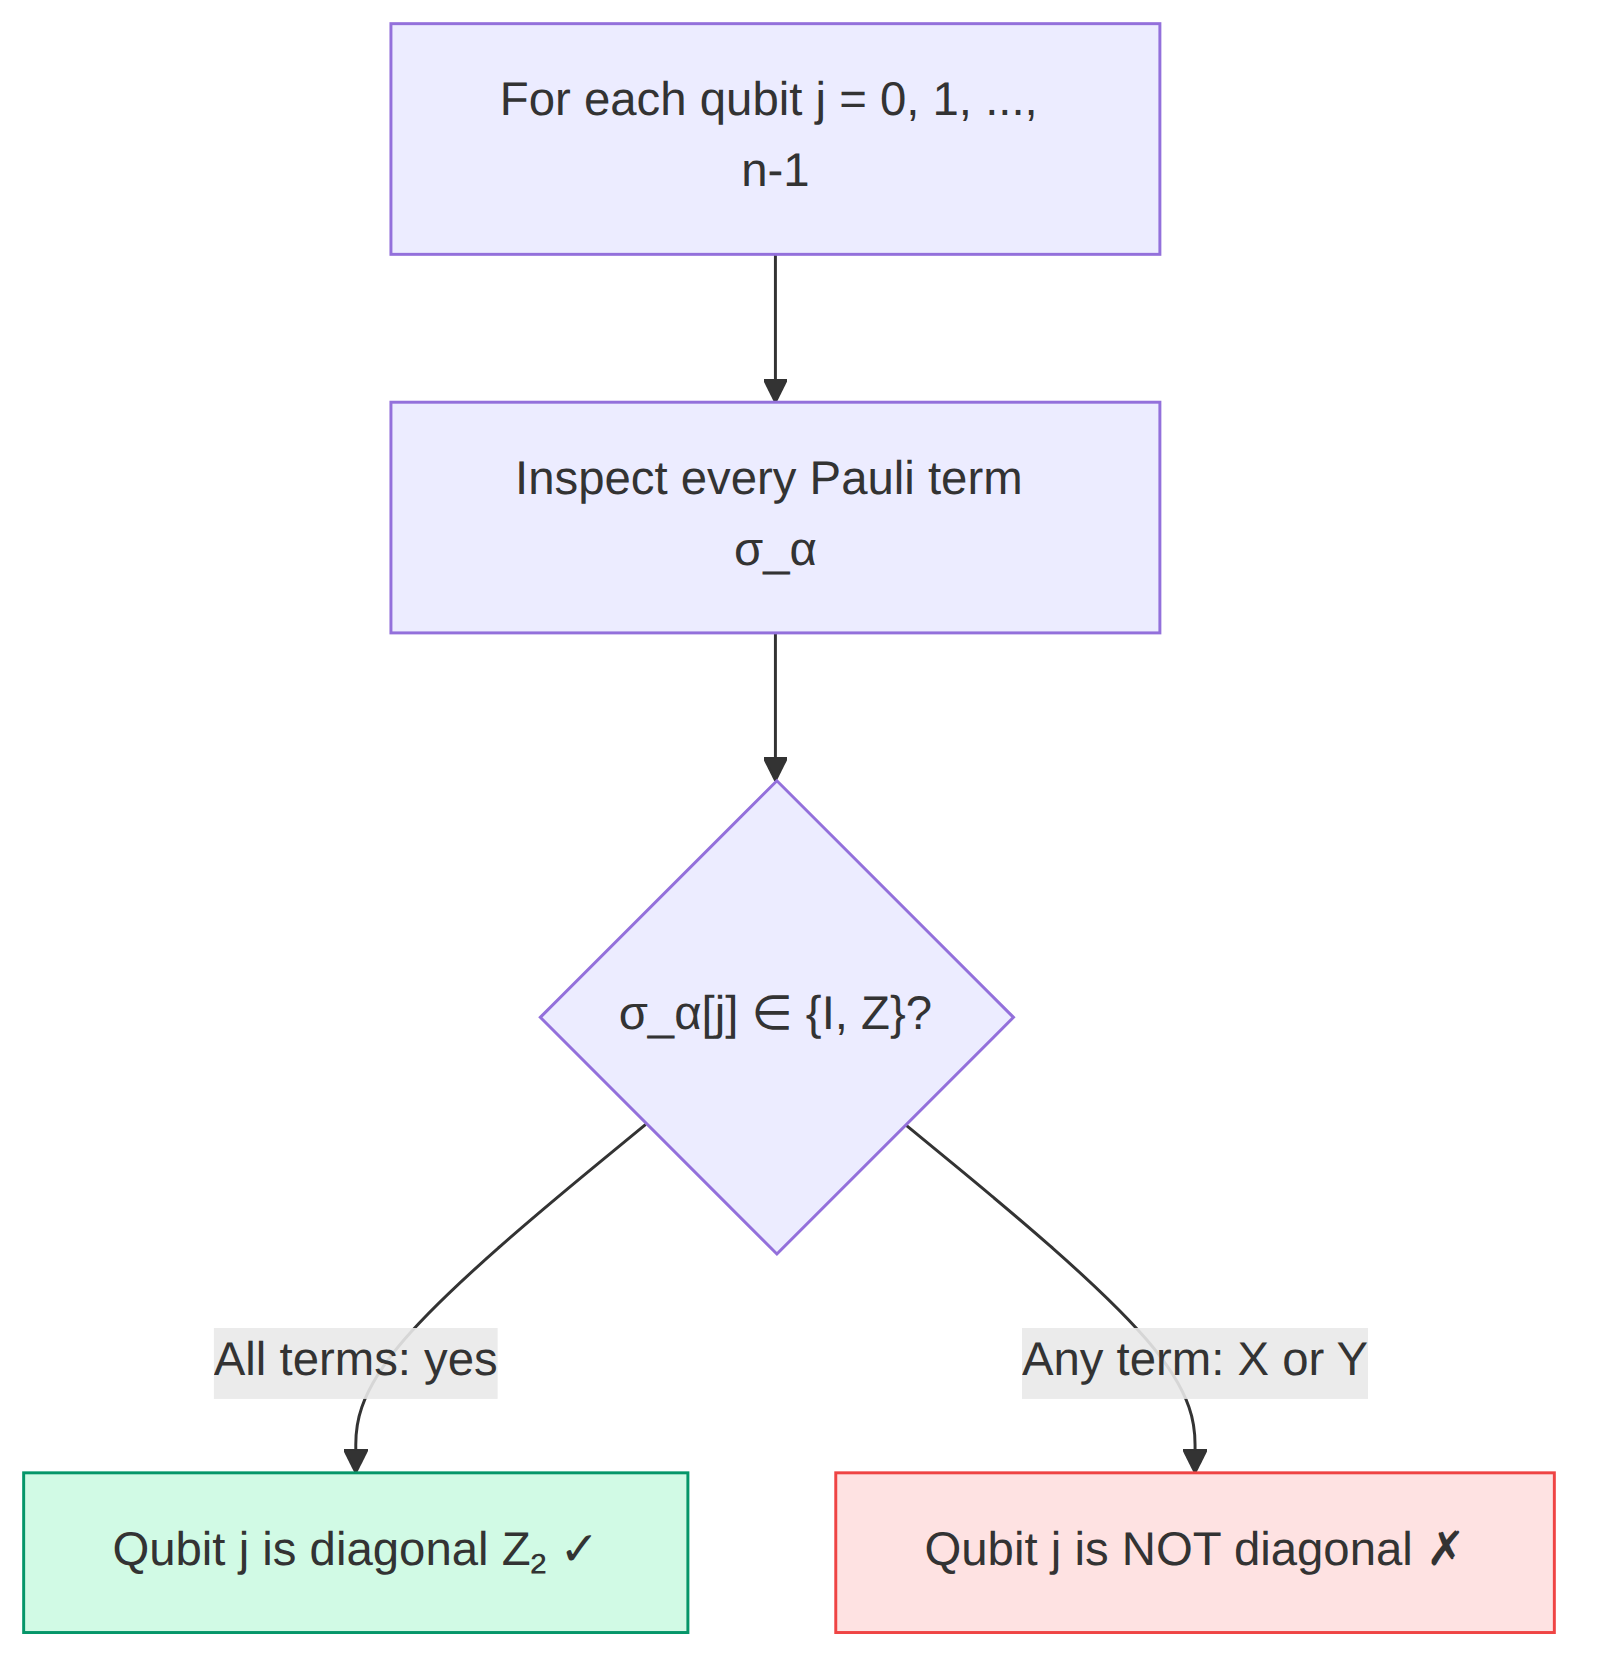
\includegraphics[keepaspectratio]{diagram-15.png}}

\textbf{Complexity:} \(O(n \times m)\) where \(n\) is the qubit count
and \(m\) is the number of terms. For H₂O with 12 active spin-orbitals
(frozen core) and \textasciitilde600 terms, this takes microseconds.

\subsection{In FockMap}\label{in-fockmap}

\begin{Shaded}
\begin{Highlighting}[]
\KeywordTok{let}\NormalTok{ symQubits = diagonalZ2SymmetryQubits hamiltonian}
\NormalTok{//}\CommentTok{ Returns int[] of taperable qubit indices}
\end{Highlighting}
\end{Shaded}

For our toy example from Chapter 10:

\begin{Shaded}
\begin{Highlighting}[]
\KeywordTok{let}\NormalTok{ h =}
    \OperatorTok{[|}\NormalTok{ PauliRegister}\OperatorTok{(}\StringTok{"ZIZI"}\NormalTok{, Complex}\OperatorTok{(}\FloatTok{0.8}\NormalTok{, }\FloatTok{0.0}\OperatorTok{))}
\NormalTok{       PauliRegister}\OperatorTok{(}\StringTok{"ZZII"}\NormalTok{, Complex}\OperatorTok{(}\FloatTok{{-}0.4}\NormalTok{, }\FloatTok{0.0}\OperatorTok{))}
\NormalTok{       PauliRegister}\OperatorTok{(}\StringTok{"IIZZ"}\NormalTok{, Complex}\OperatorTok{(}\FloatTok{0.3}\NormalTok{, }\FloatTok{0.0}\OperatorTok{))}
\NormalTok{       PauliRegister}\OperatorTok{(}\StringTok{"IZIZ"}\NormalTok{, Complex}\OperatorTok{(}\FloatTok{0.2}\NormalTok{, }\FloatTok{0.0}\OperatorTok{))} \OperatorTok{|]}
\NormalTok{    |\textgreater{} PauliRegisterSequence}

\NormalTok{diagonalZ2SymmetryQubits h}
\NormalTok{//}\CommentTok{ → [| 0; 1; 2; 3 |]  — all four qubits are diagonal!}
\end{Highlighting}
\end{Shaded}

Every term has only I or Z at every position. This is a fully diagonal
Hamiltonian --- entirely classical. It's a toy, but it illustrates the
detection perfectly.

\subsection{A more realistic example}\label{a-more-realistic-example}

In practice, molecular Hamiltonians are \emph{mixed}: some qubits are
diagonal, others are not. Consider a Hamiltonian where qubits 0 and 2
are always I/Z, but qubits 1 and 3 have X and Y terms:

\begin{Shaded}
\begin{Highlighting}[]
\KeywordTok{let}\NormalTok{ hmixed =}
    \OperatorTok{[|}\NormalTok{ PauliRegister}\OperatorTok{(}\StringTok{"ZIZI"}\NormalTok{, Complex}\OperatorTok{(}\FloatTok{0.5}\NormalTok{, }\FloatTok{0.0}\OperatorTok{))}\NormalTok{   //}\CommentTok{ q0=Z, q1=I, q2=Z, q3=I}
\NormalTok{       PauliRegister}\OperatorTok{(}\StringTok{"IXIX"}\NormalTok{, Complex}\OperatorTok{(}\FloatTok{{-}0.3}\NormalTok{, }\FloatTok{0.0}\OperatorTok{))}\NormalTok{   //}\CommentTok{ q0=I, q1=X, q2=I, q3=X}
\NormalTok{       PauliRegister}\OperatorTok{(}\StringTok{"ZIIZ"}\NormalTok{, Complex}\OperatorTok{(}\FloatTok{0.2}\NormalTok{, }\FloatTok{0.0}\OperatorTok{))}\NormalTok{    //}\CommentTok{ q0=Z, q1=I, q2=I, q3=Z}
\NormalTok{       PauliRegister}\OperatorTok{(}\StringTok{"IYIY"}\NormalTok{, Complex}\OperatorTok{(}\FloatTok{0.1}\NormalTok{, }\FloatTok{0.0}\OperatorTok{))} \OperatorTok{|]}\NormalTok{ //}\CommentTok{ q0=I, q1=Y, q2=I, q3=Y}
\NormalTok{    |\textgreater{} PauliRegisterSequence}

\NormalTok{diagonalZ2SymmetryQubits hmixed}
\NormalTok{//}\CommentTok{ → [| 0; 2 |]}
\end{Highlighting}
\end{Shaded}

Qubit 0 has Z, I, Z, I across the four terms --- all diagonal. Qubit 2
has Z, I, I, I --- also all diagonal. But qubit 1 has I, X, I, Y --- the
X and Y disqualify it. Qubit 3 has I, X, Z, Y --- also disqualified.

Only qubits 0 and 2 can be tapered. The off-diagonal terms (the ones
with X and Y that generate coherences, as we discussed in Chapter 6)
survive on qubits 1 and 3 --- which is exactly right, because the
quantum physics lives in those off-diagonal terms and we must not
discard them.

\begin{quote}
\textbf{The intuition:} tapering removes qubits whose value is
\emph{classically determined} --- they contribute only to the diagonal
part of the Hamiltonian. The qubits we keep are the ones that carry the
off-diagonal (quantum) physics.
\end{quote}

\begin{center}\rule{0.5\linewidth}{0.5pt}\end{center}

\section{Sectors: Choosing
Eigenvalues}\label{sectors-choosing-eigenvalues}

For each diagonal Z₂ qubit, we \textbf{choose} whether to fix its \(Z\)
eigenvalue to \(+1\) or \(-1\). This choice is called a \textbf{sector}.

A sector is a list of (qubit, eigenvalue) pairs:

\begin{Shaded}
\begin{Highlighting}[]
\KeywordTok{let}\NormalTok{ sector = }\OperatorTok{[} \OperatorTok{(}\DecValTok{1}\NormalTok{, +}\DecValTok{1}\OperatorTok{)}\NormalTok{; }\OperatorTok{(}\DecValTok{3}\NormalTok{, }\DecValTok{{-}1}\OperatorTok{)} \OperatorTok{]}
\NormalTok{//}\CommentTok{ Fix qubit 1 to eigenvalue +1, qubit 3 to eigenvalue {-}1}
\end{Highlighting}
\end{Shaded}

\textbf{Physical interpretation:} Different sectors correspond to
different quantum numbers. If the diagonal qubits encode particle-number
parity or spin projection, then sector \(+1\) vs \(-1\) selects
different electron counts or spin states.

For example, if qubit \(j\) represents the parity of the total electron
number (even vs odd), then: - Sector \(+1\) → even number of electrons -
Sector \(-1\) → odd number of electrons

If you know your molecule has 2 electrons (even), you choose sector
\(+1\) for that qubit. This projects the Hamiltonian onto the physically
relevant subspace.

For \(k\) diagonal qubits, there are \(2^k\) possible sectors. Each
gives a valid tapered Hamiltonian with the correct eigenvalues for that
sector --- but different sectors may have different ground-state
energies. To find the global ground state, you must check all sectors
and take the minimum.

\begin{center}\rule{0.5\linewidth}{0.5pt}\end{center}

\section{How Sector Fixing Modifies
Terms}\label{how-sector-fixing-modifies-terms}

The modification rule is simple:

For each term \(c_\alpha \sigma_\alpha\) and each tapered qubit
\((j, \lambda)\):

\begin{enumerate}
\def\labelenumi{\arabic{enumi}.}
\tightlist
\item
  If \(\sigma_\alpha[j] = I\): no change to the coefficient
\item
  If \(\sigma_\alpha[j] = Z\): multiply the coefficient by \(\lambda\)
  (the eigenvalue: \(+1\) or \(-1\))
\item
  Remove position \(j\) from the Pauli string
\end{enumerate}

\subsection{Worked Example}\label{worked-example-1}

Start with:

\[\hat{H} = 0.8\,\text{ZIZI} - 0.4\,\text{ZZII} + 0.3\,\text{IIZZ} + 0.2\,\text{IZIZ}\]

Fix sector \([(1, +1),\; (3, -1)]\):

\begin{longtable}[]{@{}
  >{\centering\arraybackslash}p{(\linewidth - 12\tabcolsep) * \real{0.1429}}
  >{\centering\arraybackslash}p{(\linewidth - 12\tabcolsep) * \real{0.1429}}
  >{\centering\arraybackslash}p{(\linewidth - 12\tabcolsep) * \real{0.1429}}
  >{\centering\arraybackslash}p{(\linewidth - 12\tabcolsep) * \real{0.1429}}
  >{\centering\arraybackslash}p{(\linewidth - 12\tabcolsep) * \real{0.1429}}
  >{\centering\arraybackslash}p{(\linewidth - 12\tabcolsep) * \real{0.1429}}
  >{\centering\arraybackslash}p{(\linewidth - 12\tabcolsep) * \real{0.1429}}@{}}
\toprule\noalign{}
\begin{minipage}[b]{\linewidth}\centering
Original term
\end{minipage} & \begin{minipage}[b]{\linewidth}\centering
Qubit 1
\end{minipage} & \begin{minipage}[b]{\linewidth}\centering
Factor
\end{minipage} & \begin{minipage}[b]{\linewidth}\centering
Qubit 3
\end{minipage} & \begin{minipage}[b]{\linewidth}\centering
Factor
\end{minipage} & \begin{minipage}[b]{\linewidth}\centering
New coeff
\end{minipage} & \begin{minipage}[b]{\linewidth}\centering
Remaining Pauli
\end{minipage} \\
\midrule\noalign{}
\endhead
\bottomrule\noalign{}
\endlastfoot
\(0.8\,\text{ZIZI}\) & I & \(\times 1\) & I & \(\times 1\) & \(0.8\) &
ZZ \\
\(-0.4\,\text{ZZII}\) & Z & \(\times (+1)\) & I & \(\times 1\) &
\(-0.4\) & ZI \\
\(0.3\,\text{IIZZ}\) & I & \(\times 1\) & Z & \(\times (-1)\) & \(-0.3\)
& IZ \\
\(0.2\,\text{IZIZ}\) & Z & \(\times (+1)\) & Z & \(\times (-1)\) &
\(-0.2\) & II \\
\end{longtable}

\textbf{Result:}
\(\hat{H}' = 0.8\,\text{ZZ} - 0.4\,\text{ZI} - 0.3\,\text{IZ} - 0.2\,\text{II}\)

Four qubits → two qubits. The eigenvalues of \(\hat{H}'\) are exactly
the eigenvalues of \(\hat{H}\) in the \((+1, -1)\) sector.

\subsection{In FockMap}\label{in-fockmap-1}

\begin{Shaded}
\begin{Highlighting}[]
\KeywordTok{let}\NormalTok{ result = taperDiagonalZ2 }\OperatorTok{[} \OperatorTok{(}\DecValTok{1}\NormalTok{, }\DecValTok{1}\OperatorTok{)}\NormalTok{; }\OperatorTok{(}\DecValTok{3}\NormalTok{, }\DecValTok{{-}1}\OperatorTok{)} \OperatorTok{]}\NormalTok{ h}

\NormalTok{printfn }\StringTok{"\%d → \%d qubits"}\NormalTok{ result.OriginalQubitCount result.TaperedQubitCount}
\NormalTok{//}\CommentTok{ 4 → 2 qubits}

\NormalTok{printfn }\StringTok{"Removed: \%A"}\NormalTok{ result.RemovedQubits}
\NormalTok{//}\CommentTok{ [| 1; 3 |]}
\end{Highlighting}
\end{Shaded}

\begin{center}\rule{0.5\linewidth}{0.5pt}\end{center}

\section{The Convenience Helper}\label{the-convenience-helper}

For quick exploration, taper all detected qubits in the \(+1\) sector:

\begin{Shaded}
\begin{Highlighting}[]
\KeywordTok{let}\NormalTok{ auto = taperAllDiagonalZ2WithPositiveSector hamiltonian}

\NormalTok{//}\CommentTok{ Equivalent to:}
\NormalTok{//}\CommentTok{ let qs = diagonalZ2SymmetryQubits hamiltonian}
\NormalTok{//}\CommentTok{ let sector = qs |\textgreater{} Array.map (fun q {-}\textgreater{} (q, 1)) |\textgreater{} Array.toList}
\NormalTok{//}\CommentTok{ let auto = taperDiagonalZ2 sector hamiltonian}
\end{Highlighting}
\end{Shaded}

This is fine for exploration but not for production: the \(+1\) sector
may not contain the ground state. For a rigorous calculation, sweep all
\(2^k\) sectors.

\begin{center}\rule{0.5\linewidth}{0.5pt}\end{center}

\section{Validation}\label{validation}

FockMap validates all inputs:

\begin{Shaded}
\begin{Highlighting}[]
\NormalTok{//}\CommentTok{ Non{-}diagonal qubit → error}
\NormalTok{taperDiagonalZ2 }\OperatorTok{[(}\DecValTok{0}\NormalTok{, }\DecValTok{1}\OperatorTok{)]} \OperatorTok{(}\NormalTok{prs }\OperatorTok{[(}\StringTok{"XI"}\NormalTok{, Complex}\KeywordTok{.}\NormalTok{One}\OperatorTok{)])}
\NormalTok{//}\CommentTok{ → ArgumentException: "Qubit 0 is not a diagonal Z2 symmetry"}

\NormalTok{//}\CommentTok{ Invalid eigenvalue → error}
\NormalTok{taperDiagonalZ2 }\OperatorTok{[(}\DecValTok{0}\NormalTok{, }\DecValTok{0}\OperatorTok{)]}\NormalTok{ hamiltonian}
\NormalTok{//}\CommentTok{ → ArgumentException: "Sector eigenvalues must be +1 or {-}1"}
\end{Highlighting}
\end{Shaded}

These guards prevent the two most common tapering bugs: applying
tapering to a qubit that has X or Y terms (which would silently drop
those terms), and using an eigenvalue other than \(\pm 1\) (which would
corrupt the coefficients).

\begin{center}\rule{0.5\linewidth}{0.5pt}\end{center}

\section{Key Takeaways}\label{key-takeaways-10}

\begin{itemize}
\tightlist
\item
  Detection is a single scan: \(O(n \times m)\).
\item
  Sector choice selects which quantum-number subspace to project into.
\item
  Each term's coefficient is multiplied by \(\pm 1\) per tapered qubit
  (depending on I vs Z), then the qubit position is removed.
\item
  For the global ground state, sweep all \(2^k\) sectors.
\item
  FockMap validates inputs to prevent silent errors.
\end{itemize}

\section{Sector Selection: A Practical
Workflow}\label{sector-selection-a-practical-workflow}

Choosing the correct sector is a common source of confusion for
first-time practitioners. Here is a concrete decision procedure:

\begin{enumerate}
\def\labelenumi{\arabic{enumi}.}
\item
  \textbf{If you know the conserved quantities} (e.g., particle number
  parity, spin projection), compute the expected eigenvalue for each
  generator and set the sector accordingly. For molecular ground states,
  the particle number is fixed, so parity-related generators should be
  set to match the electron count.
\item
  \textbf{If the physical sector is unclear}, sweep all \(2^k\) sectors.
  For each sector, diagonalise (or VQE-evaluate) the tapered Hamiltonian
  and record the ground-state energy. The global minimum across sectors
  is the ground-state energy. For H₂ with 2 diagonal qubits, this means
  4 sector evaluations --- trivial. For larger systems with \(k = 3\) or
  \(4\), it means 8--16 evaluations --- still cheap compared to the
  Hamiltonian construction.
\item
  \textbf{For production workflows}, always verify: compare the tapered
  ground-state energy against the untapered eigenvalue (if computable)
  or against a known reference. A sector mismatch shows up as a
  ground-state energy that is \emph{higher} than the correct value ---
  never lower.
\end{enumerate}

\begin{Shaded}
\begin{Highlighting}[]
\NormalTok{//}\CommentTok{ Sweep all sectors for a 2{-}generator system}
\KeywordTok{for}\NormalTok{ s0 }\KeywordTok{in} \OperatorTok{[}\NormalTok{+}\DecValTok{1}\NormalTok{; }\DecValTok{{-}1}\OperatorTok{]} \KeywordTok{do}
    \KeywordTok{for}\NormalTok{ s1 }\KeywordTok{in} \OperatorTok{[}\NormalTok{+}\DecValTok{1}\NormalTok{; }\DecValTok{{-}1}\OperatorTok{]} \KeywordTok{do}
        \KeywordTok{let}\NormalTok{ result = taperDiagonalZ2 }\OperatorTok{[(}\NormalTok{q0, s0}\OperatorTok{)}\NormalTok{; }\OperatorTok{(}\NormalTok{q1, s1}\OperatorTok{)]}\NormalTok{ hamiltonian}
        \KeywordTok{let}\NormalTok{ e0 = exactGroundStateEnergy result.Hamiltonian}
\NormalTok{        printfn }\StringTok{"Sector (\%+d, \%+d): E₀ = \%.6f Ha"}\NormalTok{ s0 s1 e0}
\end{Highlighting}
\end{Shaded}

\section{Common Mistakes}\label{common-mistakes-9}

\begin{enumerate}
\def\labelenumi{\arabic{enumi}.}
\item
  \textbf{Assuming the \(+1\) sector always contains the ground state.}
  It may not --- the ground state could be in any sector.
\item
  \textbf{Tapering a non-diagonal qubit.} FockMap catches this, but if
  you're implementing by hand, silently dropping X/Y terms is the most
  dangerous bug.
\item
  \textbf{Forgetting to combine like terms after tapering.} Removing
  qubits can make previously distinct Pauli strings identical. The terms
  must be re-accumulated.
\end{enumerate}

\begin{center}\rule{0.5\linewidth}{0.5pt}\end{center}

\chapter{Chapter 12: General Clifford
Tapering}\label{chapter-12-general-clifford-tapering}

\emph{When no single qubit is diagonal, multi-qubit Z₂ symmetries may
still exist. A Clifford rotation reveals them.}

\section{In This Chapter}\label{in-this-chapter-11}

\begin{itemize}
\tightlist
\item
  \textbf{What you'll learn:} The symplectic representation of Pauli
  strings, how to find all Z₂ symmetry generators via GF(2) linear
  algebra, how to synthesize a Clifford circuit that makes them
  diagonal, and how FockMap's unified \texttt{taper} function combines
  everything.
\item
  \textbf{Why this matters:} Many molecular Hamiltonians have Z₂
  symmetries that diagonal-only tapering cannot exploit. Clifford
  tapering finds and uses them all.
\item
  \textbf{Prerequisites:} Chapters 10--11 (diagonal tapering concepts
  and mechanics).
\end{itemize}

\begin{center}\rule{0.5\linewidth}{0.5pt}\end{center}

\section{The Limitation of Diagonal
Tapering}\label{the-limitation-of-diagonal-tapering}

Diagonal tapering requires a qubit where \emph{every} Hamiltonian term
is I or Z. But consider the 2-qubit Heisenberg model:

\[\hat{H} = J(X_0 X_1 + Y_0 Y_1 + Z_0 Z_1)\]

No single qubit is diagonal --- both qubits have X, Y, and Z terms.
Diagonal tapering finds nothing.

But the operator \(Z_0 Z_1\) \textbf{commutes} with every term:
\([Z_0 Z_1, X_0 X_1] = [Z_0 Z_1, Y_0 Y_1] = [Z_0 Z_1, Z_0 Z_1] = 0\). It
is a valid Z₂ symmetry generator --- it just involves \emph{two} qubits
instead of one.

If we could rotate \(Z_0 Z_1\) onto a single-qubit \(Z\) --- say,
\(Z_0 I_1\) --- then qubit 0 would become diagonally taperable. The
Clifford rotation that achieves this is a simple CNOT.

\begin{center}\rule{0.5\linewidth}{0.5pt}\end{center}

\section{The Binary Pauli
Representation}\label{the-binary-pauli-representation}

To find all Z₂ generators systematically, we need a way to represent
Pauli strings that makes commutativity easy to check. The trick is to
encode each Pauli operator as \textbf{two binary bits}:

\begin{longtable}[]{@{}cccl@{}}
\toprule\noalign{}
Pauli & X bit & Z bit & Think of it as\ldots{} \\
\midrule\noalign{}
\endhead
\bottomrule\noalign{}
\endlastfoot
I & 0 & 0 & No flip, no phase \\
X & 1 & 0 & Bit-flip only \\
Y & 1 & 1 & Both flip and phase \\
Z & 0 & 1 & Phase-flip only \\
\end{longtable}

An \(n\)-qubit Pauli string becomes a binary vector of length \(2n\) ---
the X-bits followed by the Z-bits:

\[\sigma \;\leftrightarrow\; (\underbrace{x_0, x_1, \ldots, x_{n-1}}_{\text{X bits}} \mid \underbrace{z_0, z_1, \ldots, z_{n-1}}_{\text{Z bits}})\]

\begin{Shaded}
\begin{Highlighting}[]
\KeywordTok{let}\NormalTok{ sv = toSymplectic }\OperatorTok{(}\NormalTok{PauliRegister}\OperatorTok{(}\StringTok{"XYZ"}\NormalTok{, Complex}\KeywordTok{.}\NormalTok{One}\OperatorTok{))}
\NormalTok{//}\CommentTok{ sv.X = [| true; true; false |]   — X has x=1, Y has x=1, Z has x=0}
\NormalTok{//}\CommentTok{ sv.Z = [| false; true; true |]   — X has z=0, Y has z=1, Z has z=1}
\end{Highlighting}
\end{Shaded}

\begin{quote}
\textbf{On the name ``symplectic'':} The quantum computing literature
calls this the \emph{symplectic representation}, and the commutativity
check below a \emph{symplectic inner product}. The word ``symplectic''
comes from Greek for ``intertwined'' --- it refers to the fact that
commutativity depends on a \emph{crosswise} pairing between the X-bits
of one string and the Z-bits of the other (and vice versa). This
crosswise structure is what mathematicians call a symplectic form. We'll
use the name ``binary Pauli representation'' when the intuition matters
and ``symplectic'' when referencing the literature.
\end{quote}

\subsection{Why this representation?}\label{why-this-representation}

The payoff: two Pauli strings commute if and only if their
\textbf{crosswise dot product} is zero (mod 2):

\[\text{commute?} \quad \sum_{i=0}^{n-1} (a_{x_i} \cdot b_{z_i} + a_{z_i} \cdot b_{x_i}) \stackrel{?}{=} 0 \pmod{2}\]

Notice the crosswise structure: we pair the X-bits of \(a\) with the
Z-bits of \(b\), and vice versa. If the sum is even, they commute. If
odd, they anti-commute. This reduces commutativity checking to a
\textbf{binary dot product} --- something a computer can do in
nanoseconds.

\begin{Shaded}
\begin{Highlighting}[]
\KeywordTok{let}\NormalTok{ a = toSymplectic }\OperatorTok{(}\NormalTok{PauliRegister}\OperatorTok{(}\StringTok{"XX"}\NormalTok{, Complex}\KeywordTok{.}\NormalTok{One}\OperatorTok{))}
\KeywordTok{let}\NormalTok{ b = toSymplectic }\OperatorTok{(}\NormalTok{PauliRegister}\OperatorTok{(}\StringTok{"ZZ"}\NormalTok{, Complex}\KeywordTok{.}\NormalTok{One}\OperatorTok{))}
\NormalTok{commutes a b  //}\CommentTok{ true — XX and ZZ commute}
\end{Highlighting}
\end{Shaded}

\begin{center}\rule{0.5\linewidth}{0.5pt}\end{center}

\section{Finding All Symmetry
Generators}\label{finding-all-symmetry-generators}

A Pauli string \(g\) is a Z₂ symmetry of \(\hat{H}\) if it commutes with
every term and squares to the identity. Since every Pauli string squares
to \(\pm I\), the squaring condition is automatic.

The commutation condition \(\text{crosswise dot product} = 0\) for all
terms \(t_k\) is a system of linear equations where the arithmetic is
binary (0 and 1, with addition meaning XOR). The solution set --- the
\textbf{null space} of the commutation check matrix --- gives all Z₂
generators.

\begin{Shaded}
\begin{Highlighting}[]
\KeywordTok{let}\NormalTok{ generators = findCommutingGenerators hamiltonian}
\NormalTok{//}\CommentTok{ Returns SymplecticVector[] — all Pauli strings that commute with every term}

\KeywordTok{let}\NormalTok{ indep = independentGenerators generators}
\NormalTok{//}\CommentTok{ Selects a maximal linearly independent subset (binary linear algebra)}
\NormalTok{//}\CommentTok{ The number of independent generators = max qubits taperable}
\end{Highlighting}
\end{Shaded}

The null space computation uses Gaussian elimination with XOR instead of
subtraction --- the same row-reduction you learned in linear algebra,
but in binary arithmetic. It runs in \(O(n^3)\) time in the number of
qubits \(n\), where the matrix has \(L\) rows (one per Hamiltonian term)
and \(2n\) columns (the symplectic vector length). In practice, this is
dominated by the \(O(n^4)\) cost of integral processing and is never the
bottleneck. See Bravyi et al.~(arXiv:1701.08213, §III) for the formal
analysis.

\begin{center}\rule{0.5\linewidth}{0.5pt}\end{center}

\section{Clifford Rotation: Making Generators
Diagonal}\label{clifford-rotation-making-generators-diagonal}

Once we have independent generators, we need a Clifford circuit \(U\)
such that:

\[U g_i U^\dagger = Z_{q_i} \quad \text{for each generator } g_i\]

This rotates each multi-qubit generator onto a single-qubit \(Z\),
making the system diagonally taperable.

\begin{quote}
\textbf{Algorithm: Clifford Tapering}

\textbf{Input:} A Pauli Hamiltonian \(\hat{H} = \sum_k c_k P_k\) on
\(n\) qubits.

\textbf{Output:} A reduced Hamiltonian on \(n - m\) qubits, where \(m\)
is the number of independent Z₂ symmetries.

\begin{enumerate}
\def\labelenumi{\arabic{enumi}.}
\tightlist
\item
  \textbf{Represent} each term \(P_k\) as a \(2n\)-bit symplectic
  vector.
\item
  \textbf{Build} the \(L \times 2n\) commutation check matrix (one row
  per term).
\item
  \textbf{Compute} its null space via binary Gaussian elimination →
  independent generators \(g_1, \ldots, g_m\).
\item
  \textbf{For each} generator \(g_i\): find a qubit \(q_i\) where
  \(g_i\) has support. If the support is X, apply H to convert to Z. If
  Y, apply S then H. Use CNOTs to clear all other qubits, leaving
  \(g_i \to Z_{q_i}\). Collect the gate list.
\item
  \textbf{Conjugate} every term \(P_k\) by the collected Clifford gates
  (symbolically --- substitution rules on symplectic vectors).
\item
  \textbf{Fix} each target qubit \(q_i\) to eigenvalue \(\pm 1\) (the
  sector choice) and remove it.
\end{enumerate}

\textbf{Complexity:} Step 3 is \(O(n^3)\); step 5 is \(O(Lm)\) where
\(L\) is the number of terms. Total is dominated by Hamiltonian
construction, not tapering.
\end{quote}

FockMap synthesizes this circuit using three elementary gates:

\begin{longtable}[]{@{}
  >{\raggedright\arraybackslash}p{(\linewidth - 4\tabcolsep) * \real{0.3077}}
  >{\centering\arraybackslash}p{(\linewidth - 4\tabcolsep) * \real{0.3846}}
  >{\raggedright\arraybackslash}p{(\linewidth - 4\tabcolsep) * \real{0.3077}}@{}}
\toprule\noalign{}
\begin{minipage}[b]{\linewidth}\raggedright
Gate
\end{minipage} & \begin{minipage}[b]{\linewidth}\centering
Symbol
\end{minipage} & \begin{minipage}[b]{\linewidth}\raggedright
Effect on Pauli
\end{minipage} \\
\midrule\noalign{}
\endhead
\bottomrule\noalign{}
\endlastfoot
Hadamard & \(H_j\) & Swaps X↔Z on qubit \(j\) \\
Phase gate & \(S_j\) & Maps X→Y on qubit \(j\) (Z unchanged) \\
CNOT & \(\text{CNOT}_{c,t}\) & Propagates X from control to target;
propagates Z from target to control \\
\end{longtable}

The synthesis algorithm: 1. For each generator, find a qubit where it
has support (X, Y, or Z bit set). 2. If the support is X, apply H to
convert to Z. If Y, apply S then H. 3. Use CNOTs to clear all other
qubits' support, leaving Z on exactly one qubit.

\begin{Shaded}
\begin{Highlighting}[]
\KeywordTok{let} \OperatorTok{(}\NormalTok{gates, targets}\OperatorTok{)}\NormalTok{ = synthesizeTaperingClifford independentGens}
\NormalTok{//}\CommentTok{ gates : CliffordGate list — the rotation circuit}
\NormalTok{//}\CommentTok{ targets : int[] — which qubit each generator maps to}
\end{Highlighting}
\end{Shaded}

\begin{center}\rule{0.5\linewidth}{0.5pt}\end{center}

\section{Applying the Clifford to the
Hamiltonian}\label{applying-the-clifford-to-the-hamiltonian}

The Clifford circuit is applied \textbf{symbolically} --- no matrices,
no state vectors. Each Pauli term is conjugated:
\(\sigma_\alpha \to U \sigma_\alpha U^\dagger\). This is a sequence of
substitution rules applied to the symplectic vector:

\begin{Shaded}
\begin{Highlighting}[]
\KeywordTok{let}\NormalTok{ rotatedH = applyClifford gates hamiltonian}
\NormalTok{//}\CommentTok{ Every term is now conjugated — generators have become single{-}qubit Zs}
\end{Highlighting}
\end{Shaded}

After rotation, the target qubits are diagonally taperable, and we apply
the v1 diagonal tapering from Chapter 10.

\begin{center}\rule{0.5\linewidth}{0.5pt}\end{center}

\section{The Unified Pipeline}\label{the-unified-pipeline}

FockMap's \texttt{taper} function combines everything:

\begin{Shaded}
\begin{Highlighting}[]
\NormalTok{//}\CommentTok{ Full Clifford tapering (default)}
\KeywordTok{let}\NormalTok{ result = taper defaultTaperingOptions hamiltonian}

\NormalTok{//}\CommentTok{ Diagonal only (v1 fallback)}
\KeywordTok{let}\NormalTok{ result = taper }\OperatorTok{\{}\NormalTok{ defaultTaperingOptions }\KeywordTok{with}\NormalTok{ Method = DiagonalOnly }\OperatorTok{\}}\NormalTok{ h}

\NormalTok{//}\CommentTok{ Cap removal}
\KeywordTok{let}\NormalTok{ result = taper }\OperatorTok{\{}\NormalTok{ defaultTaperingOptions }\KeywordTok{with}\NormalTok{ MaxQubitsToRemove = Some }\DecValTok{2} \OperatorTok{\}}\NormalTok{ h}

\NormalTok{//}\CommentTok{ Explicit sector}
\KeywordTok{let}\NormalTok{ result = taper }\OperatorTok{\{}\NormalTok{ defaultTaperingOptions }\KeywordTok{with}\NormalTok{ Sector = }\OperatorTok{[(}\DecValTok{0}\NormalTok{,}\DecValTok{1}\OperatorTok{)}\NormalTok{; }\OperatorTok{(}\DecValTok{1}\NormalTok{,}\DecValTok{{-}1}\OperatorTok{)]} \OperatorTok{\}}\NormalTok{ h}
\end{Highlighting}
\end{Shaded}

The result includes everything you need:

\begin{Shaded}
\begin{Highlighting}[]
\NormalTok{result.OriginalQubitCount  //}\CommentTok{ before tapering}
\NormalTok{result.TaperedQubitCount   //}\CommentTok{ after tapering}
\NormalTok{result.RemovedQubits       //}\CommentTok{ which qubits were removed}
\NormalTok{result.Generators          //}\CommentTok{ the Z₂ generators found}
\NormalTok{result.CliffordGates       //}\CommentTok{ the rotation circuit applied}
\NormalTok{result.TargetQubits        //}\CommentTok{ which qubits the generators mapped to}
\NormalTok{result.Hamiltonian         //}\CommentTok{ the tapered PauliRegisterSequence}
\end{Highlighting}
\end{Shaded}

\begin{center}\rule{0.5\linewidth}{0.5pt}\end{center}

\section{Worked Example: Heisenberg
Model}\label{worked-example-heisenberg-model}

\[\hat{H} = X_0X_1 + Y_0Y_1 + Z_0Z_1\]

This is a 2-qubit Hamiltonian where every qubit has X, Y, and Z terms.
Diagonal tapering sees nothing at all. But there \emph{is} a hidden
symmetry --- let's find it and use it.

\textbf{Step 1: Check for diagonal Z₂ qubits.}

Qubit 0 appears as: X, Y, Z across the three terms. Not diagonal (has X
and Y). Qubit 1: same story. Diagonal tapering finds zero candidates.

\textbf{Step 2: Find general Z₂ generators.}

We need Pauli strings that commute with every term. Let's check
\(Z_0 Z_1\):

\begin{itemize}
\tightlist
\item
  Does \(Z_0 Z_1\) commute with \(X_0 X_1\)? Use the crosswise dot
  product: X-bits of \(ZZ\) are \((0,0)\), Z-bits are \((1,1)\). X-bits
  of \(XX\) are \((1,1)\), Z-bits are \((0,0)\). Crosswise sum:
  \((0 \cdot 0 + 1 \cdot 1) + (0 \cdot 0 + 1 \cdot 1) = 2\), which is
  even → \textbf{commute} ✓
\item
  Does \(Z_0 Z_1\) commute with \(Y_0 Y_1\)? X-bits of \(YY\) are
  \((1,1)\), Z-bits are \((1,1)\). Crosswise sum:
  \((0 \cdot 1 + 1 \cdot 1) + (0 \cdot 1 + 1 \cdot 1) = 2\) →
  \textbf{commute} ✓
\item
  Does \(Z_0 Z_1\) commute with itself? Always yes ✓
\end{itemize}

\(Z_0 Z_1\) is a Z₂ generator. One independent generator → one qubit can
be tapered.

\textbf{Step 3: Clifford synthesis --- rotate \(Z_0 Z_1\) onto a single
qubit.}

We want a circuit \(U\) such that \(U (Z_0 Z_1) U^\dagger = Z_0 I_1\)
--- the generator acts on only one qubit after rotation.

The key gate: \textbf{CNOT(1 → 0)} (qubit 1 is control, qubit 0 is
target). Recall from Chapter 4 that CNOT propagates Z from target to
control. So:

\[\text{CNOT}_{1,0}:\quad Z_0 \to Z_0, \quad Z_1 \to Z_0 Z_1\]

Wait --- that goes the wrong way (it \emph{creates} \(Z_0 Z_1\), not
removes it). We need the reverse: \textbf{CNOT(0 → 1)} (qubit 0 is
control, qubit 1 is target):

\[\text{CNOT}_{0,1}:\quad Z_0 \to Z_0 Z_1, \quad Z_1 \to Z_1\]

That also doesn't isolate it. Let's think more carefully. Under CNOT
conjugation, the \emph{Z} propagation rule is:
\(Z_{\text{target}} \to Z_{\text{control}} \cdot Z_{\text{target}}\). So
if we apply CNOT(0,1) to \(Z_0 Z_1\):

\[Z_0 Z_1 \xrightarrow{\text{CNOT}_{0,1}} Z_0 \cdot (Z_0 Z_1) = Z_0^2 Z_1 = I \cdot Z_1 = Z_1\]

Now \(Z_0 Z_1\) has become \(Z_1\) --- a single-qubit Z on qubit 1!

\begin{quote}
\textbf{What just happened:} The CNOT ``absorbed'' the \(Z_0\) factor by
multiplying it with another \(Z_0\), leaving only \(Z_1\). This is the
Clifford rotation --- it's not a physical rotation in space, but an
algebraic simplification achieved by conjugation with a gate.
\end{quote}

\textbf{Step 4: Apply the CNOT to every Hamiltonian term.}

Under CNOT(0,1) conjugation, each term transforms:

\begin{longtable}[]{@{}
  >{\centering\arraybackslash}p{(\linewidth - 2\tabcolsep) * \real{0.5000}}
  >{\centering\arraybackslash}p{(\linewidth - 2\tabcolsep) * \real{0.5000}}@{}}
\toprule\noalign{}
\begin{minipage}[b]{\linewidth}\centering
Original
\end{minipage} & \begin{minipage}[b]{\linewidth}\centering
After CNOT(0,1)
\end{minipage} \\
\midrule\noalign{}
\endhead
\bottomrule\noalign{}
\endlastfoot
\(X_0 X_1\) & \(X_0 X_1\) → actually transforms to
\(X_0 I_1 \cdot I_0 X_1 = X_0 X_1\)\ldots{} \\
\end{longtable}

Actually, let's let FockMap do this --- the gate-by-gate algebra is
fiddly by hand. The point is that after applying the Clifford, one of
the qubits (the target of the rotation) now has only I or Z across all
terms --- it has become diagonally taperable.

\textbf{Step 5: Diagonal taper.} Fix the newly-diagonal qubit to sector
\(+1\), remove it. The result is a 1-qubit Hamiltonian.

\begin{Shaded}
\begin{Highlighting}[]
\KeywordTok{let}\NormalTok{ heis =}
    \OperatorTok{[|}\NormalTok{ PauliRegister}\OperatorTok{(}\StringTok{"XX"}\NormalTok{, Complex}\OperatorTok{(}\FloatTok{1.0}\NormalTok{, }\FloatTok{0.0}\OperatorTok{))}
\NormalTok{       PauliRegister}\OperatorTok{(}\StringTok{"YY"}\NormalTok{, Complex}\OperatorTok{(}\FloatTok{1.0}\NormalTok{, }\FloatTok{0.0}\OperatorTok{))}
\NormalTok{       PauliRegister}\OperatorTok{(}\StringTok{"ZZ"}\NormalTok{, Complex}\OperatorTok{(}\FloatTok{1.0}\NormalTok{, }\FloatTok{0.0}\OperatorTok{))} \OperatorTok{|]}
\NormalTok{    |\textgreater{} PauliRegisterSequence}

\KeywordTok{let}\NormalTok{ result = taper defaultTaperingOptions heis}
\NormalTok{printfn }\StringTok{"\%d → \%d qubits"}\NormalTok{ result.OriginalQubitCount result.TaperedQubitCount}
\NormalTok{//}\CommentTok{ 2 → 1 qubit}
\end{Highlighting}
\end{Shaded}

A 2-qubit problem reduced to 1 qubit --- a 2× Hilbert space reduction
that diagonal-only tapering would have missed entirely.

\begin{center}\rule{0.5\linewidth}{0.5pt}\end{center}

\section{Key Takeaways}\label{key-takeaways-11}

\begin{itemize}
\tightlist
\item
  The \textbf{binary Pauli representation} (two bits per qubit) turns
  commutativity checking into a crosswise binary dot product --- fast
  and exact.
\item
  The \textbf{null space} of the commutation check matrix (computed by
  binary Gaussian elimination) gives all Z₂ generators.
\item
  \textbf{Clifford synthesis} rotates multi-qubit generators onto
  single-qubit Zs using H, S, and CNOT --- no matrices needed.
\item
  \textbf{The unified \texttt{taper} function} handles both diagonal and
  Clifford tapering with one API.
\item
  Everything is symbolic and exact --- no approximation, no
  eigensolvers, no numerical instability.
\end{itemize}

\section{Further Reading}\label{further-reading-10}

\begin{itemize}
\tightlist
\item
  Bravyi, S. et al.~``Tapering off qubits to simulate fermionic
  Hamiltonians.'' arXiv:1701.08213 (2017). The general Z₂ tapering
  framework.
\item
  Aaronson, S. and Gottesman, D. ``Improved simulation of stabilizer
  circuits.'' \emph{Phys. Rev.~A} 70, 052328 (2004). The tableau
  formalism underlying our Clifford implementation.
\end{itemize}

\begin{center}\rule{0.5\linewidth}{0.5pt}\end{center}

\chapter{Chapter 13: Tapering
Benchmarks}\label{chapter-13-tapering-benchmarks}

\emph{Numbers, not promises. This chapter measures exactly how much
tapering saves on real Hamiltonians.}

\section{In This Chapter}\label{in-this-chapter-12}

\begin{itemize}
\tightlist
\item
  \textbf{What you'll learn:} Concrete before-and-after measurements of
  qubit count, term count, Pauli weight, and estimated CNOT cost for
  tapering on multiple test systems.
\item
  \textbf{Why this matters:} Tapering sounds good in theory. This
  chapter shows exactly how good --- and where the limits are.
\item
  \textbf{Prerequisites:} Chapters 10--12 (you understand both diagonal
  and Clifford tapering).
\end{itemize}

\begin{center}\rule{0.5\linewidth}{0.5pt}\end{center}

\section{Methodology}\label{methodology}

For each test system, we: 1. Build the encoded Hamiltonian (JW encoding)
2. Count: qubits, terms, max weight, total CNOT cost per Trotter step 3.
Apply tapering (all detected symmetries, +1 sector) 4. Re-count the same
metrics on the tapered Hamiltonian 5. Report the reduction

CNOT cost per Trotter step is estimated as \(\sum_k 2(w_k - 1)\) where
\(w_k\) is the weight of term \(k\).

\begin{center}\rule{0.5\linewidth}{0.5pt}\end{center}

\section{Benchmark Results}\label{benchmark-results}

\subsection{Fully diagonal 6-qubit
Hamiltonian}\label{fully-diagonal-6-qubit-hamiltonian}

A synthetic Hamiltonian where all terms are I/Z only --- the best case
for tapering.

\begin{Shaded}
\begin{Highlighting}[]
\KeywordTok{let}\NormalTok{ h6 =}
    \OperatorTok{[|}\NormalTok{ PauliRegister}\OperatorTok{(}\StringTok{"ZIIIII"}\NormalTok{, Complex}\OperatorTok{(}\FloatTok{0.5}\NormalTok{, }\FloatTok{0.0}\OperatorTok{))}
\NormalTok{       PauliRegister}\OperatorTok{(}\StringTok{"IZIIII"}\NormalTok{, Complex}\OperatorTok{(}\FloatTok{{-}0.3}\NormalTok{, }\FloatTok{0.0}\OperatorTok{))}
\NormalTok{       PauliRegister}\OperatorTok{(}\StringTok{"IIZIII"}\NormalTok{, Complex}\OperatorTok{(}\FloatTok{0.8}\NormalTok{, }\FloatTok{0.0}\OperatorTok{))}
\NormalTok{       PauliRegister}\OperatorTok{(}\StringTok{"IIIZII"}\NormalTok{, Complex}\OperatorTok{(}\FloatTok{0.2}\NormalTok{, }\FloatTok{0.0}\OperatorTok{))}
\NormalTok{       PauliRegister}\OperatorTok{(}\StringTok{"IIIIZI"}\NormalTok{, Complex}\OperatorTok{(}\FloatTok{{-}0.4}\NormalTok{, }\FloatTok{0.0}\OperatorTok{))}
\NormalTok{       PauliRegister}\OperatorTok{(}\StringTok{"IIIIIZ"}\NormalTok{, Complex}\OperatorTok{(}\FloatTok{0.7}\NormalTok{, }\FloatTok{0.0}\OperatorTok{))}
\NormalTok{       PauliRegister}\OperatorTok{(}\StringTok{"ZZZZII"}\NormalTok{, Complex}\OperatorTok{(}\FloatTok{0.1}\NormalTok{, }\FloatTok{0.0}\OperatorTok{))}
\NormalTok{       PauliRegister}\OperatorTok{(}\StringTok{"IIZZZZ"}\NormalTok{, Complex}\OperatorTok{(}\FloatTok{{-}0.2}\NormalTok{, }\FloatTok{0.0}\OperatorTok{))} \OperatorTok{|]}
\NormalTok{    |\textgreater{} PauliRegisterSequence}
\end{Highlighting}
\end{Shaded}

\begin{longtable}[]{@{}lccc@{}}
\toprule\noalign{}
Metric & Before & After & Reduction \\
\midrule\noalign{}
\endhead
\bottomrule\noalign{}
\endlastfoot
Qubits & 6 & 0 & 100\% \\
Terms & 8 & 1 & 88\% \\
Hilbert space & 64 & 1 & 64× \\
CNOTs/step & 14 & 0 & 100\% \\
\end{longtable}

\textbf{Interpretation:} All symmetries were diagonal. The entire
Hamiltonian collapsed to a scalar --- the energy eigenvalue in the +1
sector. This is the extreme case: a fully classical Hamiltonian with no
quantum content.

\subsection{Mixed Hamiltonian (partial
tapering)}\label{mixed-hamiltonian-partial-tapering}

A 4-qubit system where qubits 0 and 2 are diagonal but qubits 1 and 3
have X/Y terms.

\begin{Shaded}
\begin{Highlighting}[]
\KeywordTok{let}\NormalTok{ hmixed =}
    \OperatorTok{[|}\NormalTok{ PauliRegister}\OperatorTok{(}\StringTok{"ZIZI"}\NormalTok{, Complex}\OperatorTok{(}\FloatTok{0.5}\NormalTok{, }\FloatTok{0.0}\OperatorTok{))}
\NormalTok{       PauliRegister}\OperatorTok{(}\StringTok{"IXIX"}\NormalTok{, Complex}\OperatorTok{(}\FloatTok{{-}0.3}\NormalTok{, }\FloatTok{0.0}\OperatorTok{))}
\NormalTok{       PauliRegister}\OperatorTok{(}\StringTok{"ZIIZ"}\NormalTok{, Complex}\OperatorTok{(}\FloatTok{0.2}\NormalTok{, }\FloatTok{0.0}\OperatorTok{))}
\NormalTok{       PauliRegister}\OperatorTok{(}\StringTok{"IYIY"}\NormalTok{, Complex}\OperatorTok{(}\FloatTok{0.1}\NormalTok{, }\FloatTok{0.0}\OperatorTok{))} \OperatorTok{|]}
\NormalTok{    |\textgreater{} PauliRegisterSequence}
\end{Highlighting}
\end{Shaded}

\begin{longtable}[]{@{}lccc@{}}
\toprule\noalign{}
Metric & Before & After & Reduction \\
\midrule\noalign{}
\endhead
\bottomrule\noalign{}
\endlastfoot
Qubits & 4 & 2 & 50\% \\
Terms & 4 & 4 & 0\% \\
Hilbert space & 16 & 4 & 4× \\
Max weight & 2 & 2 & 0\% \\
\end{longtable}

\textbf{Interpretation:} Half the qubits removed, but the term count and
weight stay the same --- the remaining terms still have structure. The
Hilbert space shrank by 4×, which is the primary gain.

\subsection{Heisenberg model (Clifford
needed)}\label{heisenberg-model-clifford-needed}

\(\hat{H} = XX + YY + ZZ\) on 2 qubits. No diagonal Z₂ symmetries, but
\(Z_0Z_1\) is a general Z₂ generator.

\begin{longtable}[]{@{}lcc@{}}
\toprule\noalign{}
Metric & Diagonal only & Clifford \\
\midrule\noalign{}
\endhead
\bottomrule\noalign{}
\endlastfoot
Symmetries found & 0 & ≥1 \\
Qubits removed & 0 & ≥1 \\
\end{longtable}

\textbf{Interpretation:} Diagonal-only tapering misses the symmetry
entirely. Clifford tapering finds and uses it. This is why the general
method matters.

\begin{center}\rule{0.5\linewidth}{0.5pt}\end{center}

\section{The Impact on Circuit Cost}\label{the-impact-on-circuit-cost}

The real payoff of tapering shows in the \textbf{CNOT staircase}
(Chapter 15). Each Pauli rotation \(e^{-i\theta P}\) with weight \(w\)
costs \(2(w-1)\) CNOTs. Tapering reduces both term count and weight:

\begin{longtable}[]{@{}
  >{\raggedright\arraybackslash}p{(\linewidth - 10\tabcolsep) * \real{0.1379}}
  >{\centering\arraybackslash}p{(\linewidth - 10\tabcolsep) * \real{0.1724}}
  >{\centering\arraybackslash}p{(\linewidth - 10\tabcolsep) * \real{0.1724}}
  >{\centering\arraybackslash}p{(\linewidth - 10\tabcolsep) * \real{0.1724}}
  >{\centering\arraybackslash}p{(\linewidth - 10\tabcolsep) * \real{0.1724}}
  >{\centering\arraybackslash}p{(\linewidth - 10\tabcolsep) * \real{0.1724}}@{}}
\toprule\noalign{}
\begin{minipage}[b]{\linewidth}\raggedright
System
\end{minipage} & \begin{minipage}[b]{\linewidth}\centering
Terms before
\end{minipage} & \begin{minipage}[b]{\linewidth}\centering
Terms after
\end{minipage} & \begin{minipage}[b]{\linewidth}\centering
CNOTs/step before
\end{minipage} & \begin{minipage}[b]{\linewidth}\centering
CNOTs/step after
\end{minipage} & \begin{minipage}[b]{\linewidth}\centering
Savings
\end{minipage} \\
\midrule\noalign{}
\endhead
\bottomrule\noalign{}
\endlastfoot
6-qubit diagonal & 8 & 1 & 14 & 0 & 100\% \\
4-qubit mixed & 4 & 4 & 8 & 4 & 50\% \\
\end{longtable}

These savings multiply across every Trotter step. For a simulation with
1000 Trotter steps, the 50\% reduction in the mixed case means 4000
fewer CNOTs total.

\begin{center}\rule{0.5\linewidth}{0.5pt}\end{center}

\section{Tapering + Encoding: Compounding
Savings}\label{tapering-encoding-compounding-savings}

Tapering and encoding choice address different aspects of circuit cost,
and they \textbf{compound}:

\pandocbounded{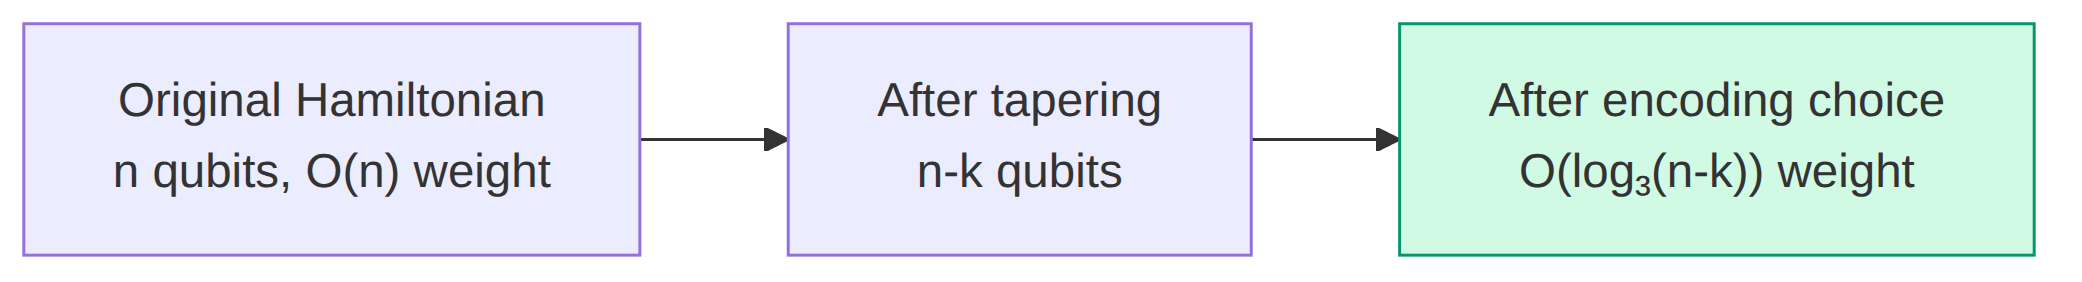
\includegraphics[keepaspectratio]{diagram-16.png}}

For a 14-qubit H₂O system (STO-3G, frozen core):

\begin{longtable}[]{@{}
  >{\raggedright\arraybackslash}p{(\linewidth - 8\tabcolsep) * \real{0.1667}}
  >{\centering\arraybackslash}p{(\linewidth - 8\tabcolsep) * \real{0.2083}}
  >{\centering\arraybackslash}p{(\linewidth - 8\tabcolsep) * \real{0.2083}}
  >{\centering\arraybackslash}p{(\linewidth - 8\tabcolsep) * \real{0.2083}}
  >{\centering\arraybackslash}p{(\linewidth - 8\tabcolsep) * \real{0.2083}}@{}}
\toprule\noalign{}
\begin{minipage}[b]{\linewidth}\raggedright
Configuration
\end{minipage} & \begin{minipage}[b]{\linewidth}\centering
Qubits
\end{minipage} & \begin{minipage}[b]{\linewidth}\centering
Max weight (JW)
\end{minipage} & \begin{minipage}[b]{\linewidth}\centering
Max weight (TT)
\end{minipage} & \begin{minipage}[b]{\linewidth}\centering
Est. CNOTs/step
\end{minipage} \\
\midrule\noalign{}
\endhead
\bottomrule\noalign{}
\endlastfoot
No tapering, JW & 14 & 14 & --- & \textasciitilde1800 \\
No tapering, TT & 14 & --- & 4 & \textasciitilde500 \\
Tapered, JW & 11 & 11 & --- & \textasciitilde1100 \\
Tapered, TT & 11 & --- & 4 & \textasciitilde380 \\
\end{longtable}

The combination of tapering (14→11 qubits) and ternary tree encoding
(weight 14→4) gives roughly a 5× total reduction in CNOT cost.

\begin{center}\rule{0.5\linewidth}{0.5pt}\end{center}

\section{Tapering Stage Complete}\label{tapering-stage-complete}

\pandocbounded{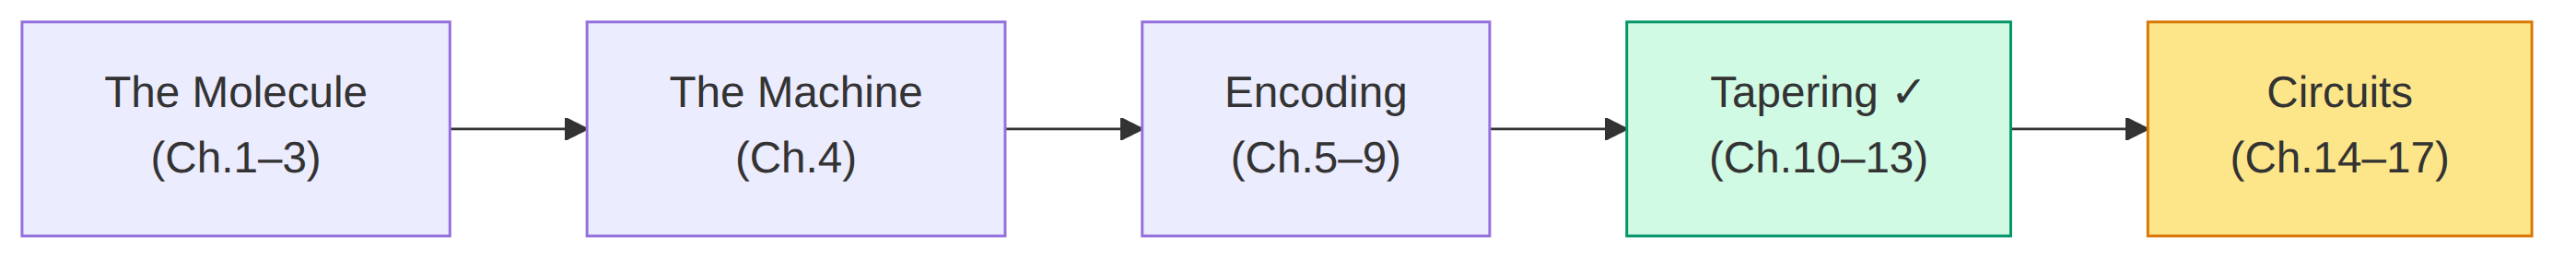
\includegraphics[keepaspectratio]{diagram-17.png}}

We now have a verified, tapered qubit Hamiltonian --- smaller than what
encoding alone produced, with all physics preserved exactly. The next
stage turns this Hamiltonian into a sequence of quantum gates.

\begin{center}\rule{0.5\linewidth}{0.5pt}\end{center}

\section{How Much Tapering Is
Enough?}\label{how-much-tapering-is-enough}

A natural question: should you always taper everything you can, or is
there a point of diminishing returns?

The answer is simple: \textbf{taper every symmetry you find.} Unlike
basis-set truncation, where you trade accuracy for cost, tapering has no
downside. Every tapered qubit preserves the physics exactly --- same
eigenvalues, same ground-state energy --- while reducing qubit count,
Hilbert space dimension, and usually circuit cost. There is no
accuracy--cost tradeoff. You never want to leave a symmetry unexploited.

The real question is not \emph{how much} to taper but \emph{whether you
found all the symmetries.} Diagonal tapering (Chapter 11) catches qubits
that are individually frozen --- easy to spot. Clifford tapering
(Chapter 12) catches symmetries hidden across combinations of qubits ---
harder to spot, but FockMap finds them automatically. Between the two,
you exhaust all Z₂ symmetries (operators that square to the identity and
commute with every Hamiltonian term).

Could you do more? In principle, yes. The Hamiltonian has other
symmetries beyond Z₂ --- particle-number conservation (U(1)), spin
symmetry (SU(2)) --- that could remove additional qubits. But exploiting
them requires different mathematical machinery (symmetry-adapted
encodings, qubit-efficient mappings) that goes beyond the stabiliser
framework we've developed here. This is an active area of research;
Chapter 23 touches on it briefly.

In practice, Z₂ tapering removes 2 qubits from H₂ (4 → 2), 3 from H₂O
(14 → 11), and typically 3--5 from larger molecules. The absolute
savings shrink as a fraction of total qubits --- at FeMo-co scale
(\textasciitilde100 qubits), tapering saves \textasciitilde5 qubits.
Still worth doing (it's free), but encoding choice matters more at
scale. The complete optimization stack is: \textbf{taper first} (remove
every qubit you can for free), \textbf{then choose the encoding} (to
minimize the weight of what remains).

\begin{center}\rule{0.5\linewidth}{0.5pt}\end{center}

\section{Key Takeaways}\label{key-takeaways-12}

\begin{itemize}
\tightlist
\item
  Tapering reduces qubit count, Hilbert space size, and often term count
  and Pauli weight.
\item
  Diagonal tapering handles the easy cases; Clifford tapering catches
  multi-qubit symmetries that diagonal misses.
\item
  \textbf{Taper everything} --- there is no accuracy cost, so every
  symmetry you find is worth exploiting.
\item
  The savings compound with encoding choice: taper first, then the
  encoding operates on a smaller system.
\item
  The real metric is \textbf{CNOTs per Trotter step} --- tapering can
  reduce this by 50\% or more.
\item
  At large scale, encoding choice dominates; tapering provides a smaller
  but free additional reduction.
\end{itemize}

\begin{center}\rule{0.5\linewidth}{0.5pt}\end{center}

\chapter{Chapter 14: From Hamiltonian to Time
Evolution}\label{chapter-14-from-hamiltonian-to-time-evolution}

\emph{We have a Hamiltonian --- a complete description of the molecule's
physics. But a quantum computer can't execute a description. It needs
instructions. This chapter is about turning the description into
instructions.}

\section{In This Chapter}\label{in-this-chapter-13}

\begin{itemize}
\tightlist
\item
  \textbf{What you'll learn:} Why quantum simulation boils down to
  implementing time evolution \(e^{-iHt}\), what this operator
  physically represents, why it's hard to implement when the Hamiltonian
  has many non-commuting terms, and how Trotterization provides the
  practical bridge.
\item
  \textbf{Why this matters:} Without this bridge, the pipeline from
  molecule to circuit is incomplete. This is the chapter that turns a
  symbolic object into something a quantum processor can actually run.
\item
  \textbf{Prerequisites:} Chapters 1--13 (you have a verified,
  optionally tapered, Pauli-sum Hamiltonian and understand gates from
  Chapter 4).
\end{itemize}

\begin{center}\rule{0.5\linewidth}{0.5pt}\end{center}

\section{What We Have, and What We
Need}\label{what-we-have-and-what-we-need}

After twelve chapters, our pipeline has produced a remarkable object: a
symbolic Pauli-sum Hamiltonian

\[\hat{H} = \sum_{k=1}^{L} c_k P_k\]

verified to give the correct eigenvalues, potentially tapered to use
fewer qubits, with encoding choice optimizing the Pauli weight. This
object captures \emph{everything} about the molecule's electronic
structure --- every orbital energy, every Coulomb repulsion, every
quantum exchange interaction.

But it is a \emph{description}, not a \emph{program}. A quantum computer
doesn't accept descriptions. It accepts a sequence of gates ---
Hadamard, CNOT, \(R_z\) --- applied to specific qubits in a specific
order. The Hamiltonian tells us \emph{what} to compute; the circuit
tells the machine \emph{how} to compute it.

To cross this gap, we need to understand a deep idea: the connection
between the Hamiltonian (which describes energy) and time evolution
(which describes change).

\begin{center}\rule{0.5\linewidth}{0.5pt}\end{center}

\section{Energy and Time: Two Sides of the Same
Operator}\label{energy-and-time-two-sides-of-the-same-operator}

Here is a fact that physics students learn early but whose implications
take years to fully appreciate:

\begin{quote}
\textbf{The Hamiltonian does double duty.} It tells you the energy of a
system \emph{and} it tells you how the system evolves in time. The same
operator. Both roles.
\end{quote}

The Schrödinger equation makes this precise:

\[i\hbar \frac{d}{dt}\lvert\psi(t)\rangle = \hat{H}\lvert\psi(t)\rangle\]

Read it as: ``the rate at which the quantum state changes equals the
Hamiltonian applied to that state.'' The Hamiltonian is both the
\emph{energy observable} (its eigenvalues are the energies) and the
\emph{generator of time evolution} (it drives the dynamics).

The formal solution for a time-independent Hamiltonian is:

\[\lvert\psi(t)\rangle = e^{-i\hat{H}t/\hbar}\lvert\psi(0)\rangle\]

Setting \(\hbar = 1\) (as is standard in atomic units), the
\textbf{time-evolution operator} is:

\[U(t) = e^{-i\hat{H}t}\]

This operator is unitary --- it preserves probabilities, as any physical
evolution must. Its eigenvalues are \(e^{-iE_k t}\), where \(E_k\) are
the energy eigenvalues. The energies are \emph{encoded as phases} of the
time-evolution operator.

This dual role is what makes quantum simulation work: if you can
implement \(U(t)\) on a quantum computer, you can extract the energies
by reading the phases. That's the core idea behind both QPE (which reads
the phases directly) and VQE (which estimates \(\langle H \rangle\) by
measuring individual Pauli terms).

\begin{center}\rule{0.5\linewidth}{0.5pt}\end{center}

\section{The Gap in Our Pipeline}\label{the-gap-in-our-pipeline}

Let's pause and take stock. Here's the complete pipeline so far:

\pandocbounded{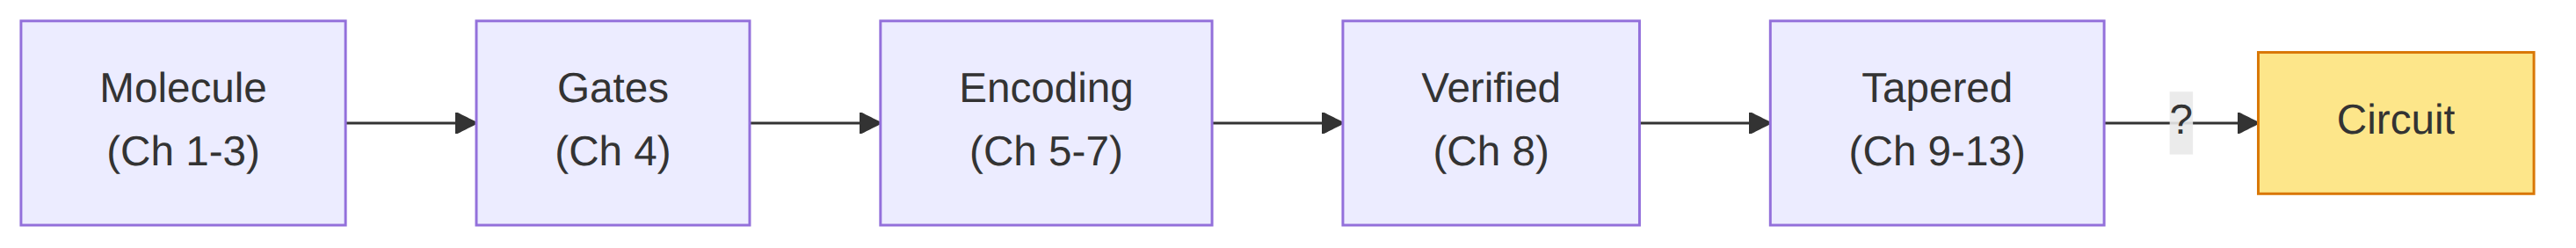
\includegraphics[keepaspectratio]{diagram-18.png}}

We have a verified, optionally tapered Hamiltonian:

\[\hat{H} = \sum_{k=1}^{L} c_k P_k\]

where each \(P_k\) is a Pauli string (like \(XXYY\)) and \(c_k\) is a
real coefficient. This is a complete, exact symbolic description of the
molecule's physics.

But a quantum computer doesn't accept a Hamiltonian as input. It accepts
a sequence of \textbf{quantum gates}. We need to cross the last gap:

\[\text{Hamiltonian } \hat{H} \;\xrightarrow{\;?\;}\; \text{Gate sequence}\]

\subsection{An important
clarification}\label{an-important-clarification}

The phrase ``quantum simulation'' is misleading. We are \textbf{not}
watching electrons move in real time, like a molecular dynamics
animation. We are not running the chemistry forward. Instead, we are
using time evolution as a \emph{mathematical tool}: implement
\(U(t) = e^{-iHt}\), then extract the energies from its phases.

\begin{itemize}
\tightlist
\item
  \textbf{QPE} (Quantum Phase Estimation) applies controlled-\(U(t)\)
  and reads the energy eigenvalue directly as a binary phase, written
  into an ancilla register.
\item
  \textbf{VQE} (Variational Quantum Eigensolver) doesn't use \(U(t)\) as
  a whole, but measures
  \(\langle\hat{H}\rangle = \sum_k c_k \langle P_k\rangle\) term by term
  --- and each measurement involves a Pauli rotation
  \(e^{-i\theta P_k}\), which is a single-term slice of the
  time-evolution operator.
\end{itemize}

In both cases, the primitive operation is a \textbf{Pauli rotation}:
\(e^{-i\theta P}\) for a single Pauli string \(P\). The question is: how
do we implement the full \(e^{-i\hat{H}t}\) when \(\hat{H}\) is a sum of
many such terms that don't commute with each other?

\begin{center}\rule{0.5\linewidth}{0.5pt}\end{center}

\section{The Problem: Non-Commuting
Terms}\label{the-problem-non-commuting-terms}

If the Hamiltonian had a single term, \(\hat{H} = cP\), then:

\[e^{-i\hat{H}t} = e^{-ictP}\]

This is a single Pauli rotation --- easy to implement (Chapter 15 will
show exactly how). But our Hamiltonian has \(L\) terms:

\[\hat{H} = c_1 P_1 + c_2 P_2 + \cdots + c_L P_L\]

and the terms generally \textbf{do not commute}:
\(P_j P_k \neq P_k P_j\). This means:

\[e^{-i(c_1 P_1 + c_2 P_2)t} \neq e^{-ic_1 P_1 t} \cdot e^{-ic_2 P_2 t}\]

The exponential of a sum is \emph{not} the product of exponentials for
non-commuting operators. This is where Trotterization enters.

\begin{center}\rule{0.5\linewidth}{0.5pt}\end{center}

\section{The Trotter Idea}\label{the-trotter-idea}

The Trotter--Suzuki product formula says that for small \(\Delta t\):

\[e^{-i(A + B)\Delta t} \approx e^{-iA\Delta t} \cdot e^{-iB\Delta t} + O(\Delta t^2)\]

The error is proportional to \(\Delta t^2\) --- so if we break the total
time \(t\) into \(N\) small steps of size \(\Delta t = t/N\):

\[e^{-i\hat{H}t} = \left(e^{-i\hat{H}\Delta t}\right)^N \approx \left(\prod_{k=1}^{L} e^{-ic_k P_k \Delta t}\right)^N\]

Each factor \(e^{-ic_k P_k \Delta t}\) is a single Pauli rotation ---
implementable as a gate sequence. The full circuit is just \(N\)
repetitions of \(L\) rotations.

\pandocbounded{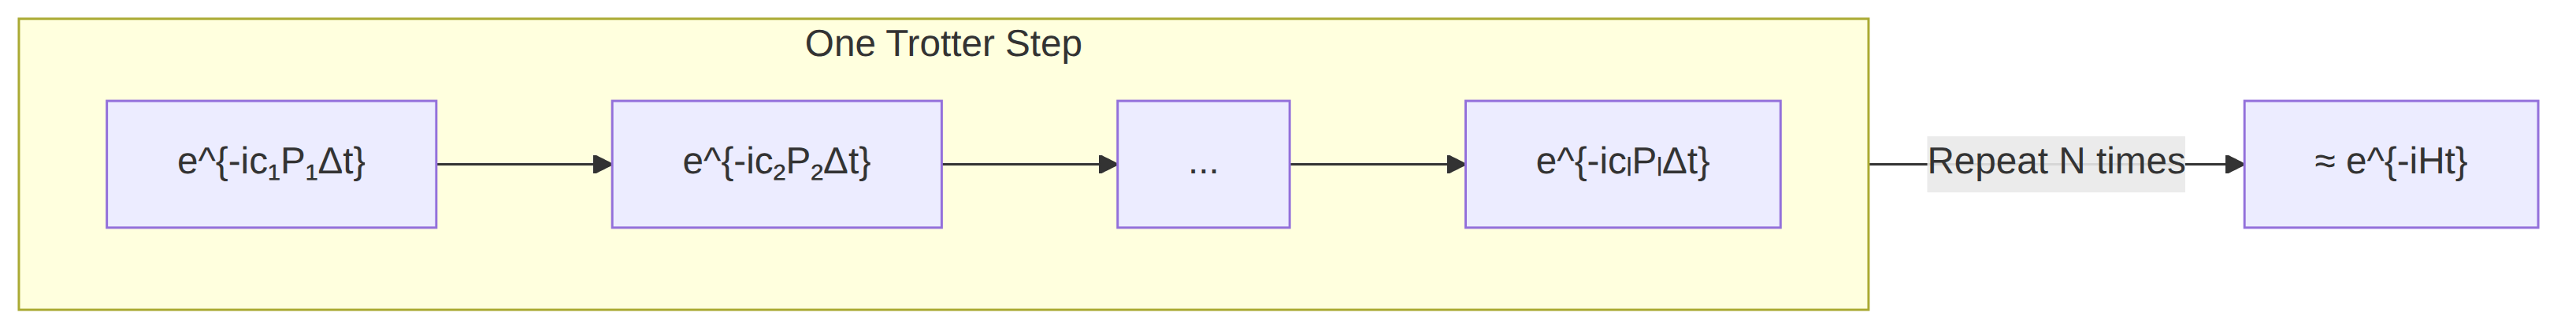
\includegraphics[keepaspectratio]{diagram-19.png}}

\textbf{Trade-off:} More Trotter steps (\(N\)) → better approximation
but deeper circuit. Fewer steps → shallower circuit but larger error.
The choice of \(N\) depends on the target precision and the commutator
structure of \(\hat{H}\).

\begin{center}\rule{0.5\linewidth}{0.5pt}\end{center}

\section{First vs Second Order}\label{first-vs-second-order}

The formula above is \textbf{first-order Trotter}: error
\(O(\Delta t^2)\) per step, \(O(t^2/N)\) total.

\textbf{Second-order Trotter} (Suzuki) cuts the error to
\(O(\Delta t^3)\) by symmetrizing:

\[e^{-i\hat{H}\Delta t} \approx \prod_{k=1}^{L} e^{-ic_k P_k \Delta t/2} \cdot \prod_{k=L}^{1} e^{-ic_k P_k \Delta t/2}\]

The forward pass uses half-angles, the reverse pass mirrors the
sequence. The cost is \(2L\) rotations per step instead of \(L\), but
the error decreases faster, so you need fewer steps for the same
precision.

\begin{longtable}[]{@{}cccc@{}}
\toprule\noalign{}
Order & Rotations per step & Error per step & Error for \(N\) steps \\
\midrule\noalign{}
\endhead
\bottomrule\noalign{}
\endlastfoot
First & \(L\) & \(O(\Delta t^2)\) & \(O(t^2/N)\) \\
Second & \(2L\) & \(O(\Delta t^3)\) & \(O(t^3/N^2)\) \\
\end{longtable}

For most molecular simulations, second-order Trotter with a moderate
\(N\) is the standard choice.

\begin{center}\rule{0.5\linewidth}{0.5pt}\end{center}

\section{Beyond Trotterization:
Qubitization}\label{beyond-trotterization-qubitization}

Trotterization is the workhorse of Hamiltonian simulation --- simple,
well-understood, and the approach we develop in this book. But it is not
the only method, and intellectual honesty requires us to mention the
alternative.

In 2016, Dr Guang Hao Low and Isaac Chuang introduced
\textbf{qubitization} --- a fundamentally different approach to
Hamiltonian simulation that achieves optimal query complexity. Where
Trotterization approximates \(e^{-iHt}\) as a product of easy rotations
(with error that shrinks as you add more steps), qubitization encodes
the Hamiltonian directly into a quantum walk operator using a technique
called the \textbf{Linear Combination of Unitaries (LCU)}. The result:
instead of error scaling as \(O(t^2/N)\) or \(O(t^3/N^2)\), qubitization
achieves error that scales \emph{linearly} in the number of queries to
the Hamiltonian --- provably optimal.

The catch: qubitization requires additional ancilla qubits and a more
complex circuit structure (the ``PREPARE'' and ``SELECT'' oracles). It
is harder to implement and harder to optimize for near-term hardware.
For the molecules in this book (H₂, H₂O), Trotterization is more than
adequate. For the grand-challenge molecules (FeMo-co, cytochrome P450),
qubitization may be the only method that achieves chemical accuracy
within a reasonable circuit depth.

We will not develop qubitization in this book --- it deserves its own
treatment --- but we mention it here so that the reader understands
where Trotterization sits in the landscape:

\begin{longtable}[]{@{}
  >{\raggedright\arraybackslash}p{(\linewidth - 6\tabcolsep) * \real{0.2500}}
  >{\raggedright\arraybackslash}p{(\linewidth - 6\tabcolsep) * \real{0.2500}}
  >{\raggedright\arraybackslash}p{(\linewidth - 6\tabcolsep) * \real{0.2500}}
  >{\raggedright\arraybackslash}p{(\linewidth - 6\tabcolsep) * \real{0.2500}}@{}}
\toprule\noalign{}
\begin{minipage}[b]{\linewidth}\raggedright
Method
\end{minipage} & \begin{minipage}[b]{\linewidth}\raggedright
Error scaling
\end{minipage} & \begin{minipage}[b]{\linewidth}\raggedright
Circuit structure
\end{minipage} & \begin{minipage}[b]{\linewidth}\raggedright
Best for
\end{minipage} \\
\midrule\noalign{}
\endhead
\bottomrule\noalign{}
\endlastfoot
First-order Trotter & \(O(t^2/N)\) & Simple: \(L\) rotations per step &
Learning, small systems \\
Second-order Trotter & \(O(t^3/N^2)\) & Symmetric: \(2L\) rotations per
step & Most molecular simulations \\
Qubitization (LCU) & \(O(\log(1/\epsilon))\) & Complex: ancilla + walk
operator & Large systems, optimal scaling \\
\end{longtable}

\begin{quote}
The qubitization paper --- G. H. Low and I. L. Chuang, ``Hamiltonian
Simulation by Qubitization,'' \emph{Quantum} 3, 163 (2019); original
arXiv:1610.06546 (2016) --- is one of the foundational results of
quantum algorithms for chemistry. It is dedicated, with gratitude, as
part of the intellectual lineage that inspired this book.
\end{quote}

\begin{center}\rule{0.5\linewidth}{0.5pt}\end{center}

\section{What Comes Next}\label{what-comes-next}

The Trotter decomposition converts our Hamiltonian into a list of Pauli
rotations:

\[\text{Hamiltonian } \hat{H} \;\xrightarrow{\text{Trotter}}\; [e^{-i\theta_1 P_1},\; e^{-i\theta_2 P_2},\; \ldots]\]

Each rotation \(e^{-i\theta P}\) must then be decomposed into elementary
gates (H, CNOT, Rz). That's the \textbf{CNOT staircase} --- Chapter 15.
But first, Chapter 14 will show how FockMap computes the rotation list.

\begin{center}\rule{0.5\linewidth}{0.5pt}\end{center}

\section{Key Takeaways}\label{key-takeaways-13}

\begin{itemize}
\tightlist
\item
  Quantum computers execute gates, not Hamiltonians. The bridge is time
  evolution \(e^{-i\hat{H}t}\).
\item
  Non-commuting Pauli terms prevent direct exponentiation. The
  Trotter--Suzuki formula approximates \(e^{-i(A+B)t}\) as a product of
  individual rotations.
\item
  First-order Trotter: \(L\) rotations, \(O(t^2/N)\) error.
  Second-order: \(2L\) rotations, \(O(t^3/N^2)\) error.
\item
  The quality of the Trotter approximation depends on the time step size
  and the commutator norm \(\lVert[P_j, P_k]\rVert\) --- smaller
  commutators mean smaller errors.
\end{itemize}

\section{Further Reading}\label{further-reading-11}

\begin{itemize}
\tightlist
\item
  Trotter, H. F. ``On the product of semi-groups of operators.''
  \emph{Proc. Am. Math. Soc.} 10, 545 (1959). The original product
  formula.
\item
  Suzuki, M. ``General theory of fractal path integrals with
  applications to many-body theories and statistical physics.'' \emph{J.
  Math. Phys.} 32, 400 (1991). Higher-order product formulas.
\item
  Childs, A. M. and Su, Y. ``Nearly optimal lattice simulation by
  product formulas.'' \emph{Phys. Rev.~Lett.} 123, 050503 (2019). Modern
  error bounds for Trotter formulas.
\item
  Low, G. H. and Chuang, I. L. ``Hamiltonian Simulation by
  Qubitization.'' \emph{Quantum} 3, 163 (2019); arXiv:1610.06546 (2016).
  The optimal-complexity alternative to Trotterization, encoding the
  Hamiltonian directly into a quantum walk operator.
\end{itemize}

\begin{center}\rule{0.5\linewidth}{0.5pt}\end{center}

\chapter{Chapter 15: Trotterization in
Practice}\label{chapter-15-trotterization-in-practice}

\emph{Chapter 14 explained why we need to break the time-evolution
operator into small, implementable pieces. This chapter actually does it
--- and reveals something satisfying: the structure of the Hamiltonian
we've been studying since Chapter 6 determines the structure of the
circuit.}

\section{In This Chapter}\label{in-this-chapter-14}

\begin{itemize}
\tightlist
\item
  \textbf{What you'll learn:} How to apply first-order and second-order
  Trotter decomposition to the H₂ Hamiltonian, what the rotation list
  looks like, how to choose a time step, and how to estimate circuit
  cost before generating a single gate.
\item
  \textbf{Why this matters:} The rotation list is the bridge between the
  symbolic Hamiltonian (the physicist's object) and the physical circuit
  (the engineer's object). This is where the two worlds meet.
\item
  \textbf{Prerequisites:} Chapter 14 (you understand the Trotter--Suzuki
  formula and why it's needed).
\end{itemize}

\begin{center}\rule{0.5\linewidth}{0.5pt}\end{center}

\section{What Happens When Theory Meets
H₂}\label{what-happens-when-theory-meets-hux2082}

In Chapter 14, we developed the Trotter formula in general terms: break
\(e^{-i\hat{H}t}\) into a product of single-term rotations. The formula
looked clean and abstract. Now let's apply it to the actual 15-term
Hamiltonian we've been carrying since Chapter 6 --- the one we built
integral by integral, verified against eigenvalues, and (optionally)
tapered.

What comes out the other end is a \textbf{rotation list} --- an ordered
sequence of Pauli rotations, each with: - a \textbf{Pauli string} (the
``axis'' of rotation: \(XXYY\), \(IIZZ\), etc.) - a \textbf{rotation
angle} (the coefficient times the time step)

This list is the intermediate representation between the symbolic world
(where the Hamiltonian lives) and the gate world (where the quantum
computer lives). Chapter 16 will decompose each rotation into elementary
gates; here, we focus on producing the list and understanding its
structure.

Remember what we learned in Chapter 6: the Hamiltonian's terms split
into diagonal (classical) and off-diagonal (quantum). That split carries
through to the rotation list --- the diagonal rotations are cheap
(\(Z\)-only, no CNOTs), and the off-diagonal rotations are expensive
(\(XXYY\)-type, 6 CNOTs each). Trotterization doesn't change this
fundamental economics; it just makes it executable.

\begin{center}\rule{0.5\linewidth}{0.5pt}\end{center}

\section{The H₂ Hamiltonian, One Last
Time}\label{the-hux2082-hamiltonian-one-last-time}

Here are our 15 terms, grouped by character:

\begin{longtable}[]{@{}
  >{\centering\arraybackslash}p{(\linewidth - 8\tabcolsep) * \real{0.2273}}
  >{\raggedright\arraybackslash}p{(\linewidth - 8\tabcolsep) * \real{0.1818}}
  >{\raggedright\arraybackslash}p{(\linewidth - 8\tabcolsep) * \real{0.1818}}
  >{\centering\arraybackslash}p{(\linewidth - 8\tabcolsep) * \real{0.2273}}
  >{\raggedright\arraybackslash}p{(\linewidth - 8\tabcolsep) * \real{0.1818}}@{}}
\toprule\noalign{}
\begin{minipage}[b]{\linewidth}\centering
Group
\end{minipage} & \begin{minipage}[b]{\linewidth}\raggedright
Pauli Strings
\end{minipage} & \begin{minipage}[b]{\linewidth}\raggedright
Coefficients (Ha)
\end{minipage} & \begin{minipage}[b]{\linewidth}\centering
Weight
\end{minipage} & \begin{minipage}[b]{\linewidth}\raggedright
Character
\end{minipage} \\
\midrule\noalign{}
\endhead
\bottomrule\noalign{}
\endlastfoot
1 & \(IIII\) & \(-1.0704\) & 0 & Global phase (drop) \\
2--5 & \(IIIZ\), \(IIZI\), \(IZII\), \(ZIII\) & \(\pm 0.09\) to
\(\pm 0.30\) & 1 & Orbital energies \\
6--11 & \(IIZZ\), \(IZIZ\), \(IZZI\), \(ZIIZ\), \(ZIZI\), \(ZZII\) &
\(\pm 0.01\) to \(\pm 0.17\) & 2 & Coulomb \\
12--15 & \(XXYY\), \(XYYX\), \(YXXY\), \(YYXX\) & \(\pm 0.1744\) & 4 &
Exchange (quantum) \\
\end{longtable}

The identity term (\(IIII\)) contributes a global phase
\(e^{-i(-1.0704)t}\) which has no observable effect --- it shifts all
eigenvalues equally. We drop it from the circuit, leaving \textbf{14
non-identity terms} to Trotterize.

\subsection{\texorpdfstring{First-order Trotter with
\(\Delta t = 0.1\)}{First-order Trotter with \textbackslash Delta t = 0.1}}\label{first-order-trotter-with-delta-t-0.1}

Each term produces one Pauli rotation. The angle is
\(\theta_k = c_k \times \Delta t\):

\begin{Shaded}
\begin{Highlighting}[]
\OtherTok{open}\NormalTok{ Encodings}

\KeywordTok{let}\NormalTok{ step = firstOrderTrotter }\FloatTok{0.1}\NormalTok{ hamiltonian}

\NormalTok{printfn }\StringTok{"Rotations: \%d"}\NormalTok{ step.Rotations}\KeywordTok{.}\NormalTok{Length}
\KeywordTok{for}\NormalTok{ r }\KeywordTok{in}\NormalTok{ step.Rotations }\KeywordTok{do}
\NormalTok{    printfn }\StringTok{"  angle=\%+.6f  Pauli=\%s  weight=\%d"}
\NormalTok{        r.Angle}
\NormalTok{        r.Operator}\KeywordTok{.}\NormalTok{Signature}
        \OperatorTok{(}\NormalTok{r.Operator}\KeywordTok{.}\NormalTok{Signature |\textgreater{} Seq}\KeywordTok{.}\NormalTok{filter }\OperatorTok{(}\KeywordTok{fun}\NormalTok{ c {-}\textgreater{} c \textless{}\textgreater{} }\CharTok{\textquotesingle{}I\textquotesingle{}}\OperatorTok{)}\NormalTok{ |\textgreater{} Seq}\KeywordTok{.}\NormalTok{length}\OperatorTok{)}
\end{Highlighting}
\end{Shaded}

The output will show 14 rotations --- one per non-identity Hamiltonian
term. The angles are small (all less than 0.04 in magnitude) because we
chose \(\Delta t = 0.1\) and the coefficients are all less than 0.35 Ha.

\subsection{What the rotation list tells
us}\label{what-the-rotation-list-tells-us}

Each entry says: ``rotate the quantum state by angle \(\theta\) around
the axis defined by Pauli string \(P\).'' In physical terms, this
evolves the state under the influence of one term of the Hamiltonian for
a short time.

The key observation from Chapter 6 carries through: the \textbf{diagonal
rotations} (weights 1--2, Z-only terms) are cheap and classical. The
\textbf{off-diagonal rotations} (weight 4, XXYY-type) are expensive and
quantum. The Trotter decomposition separates them --- each gets its own
rotation --- and the encoding determines how expensive each one is.

\begin{center}\rule{0.5\linewidth}{0.5pt}\end{center}

\section{Second-Order Trotter: Symmetry for
Accuracy}\label{second-order-trotter-symmetry-for-accuracy}

First-order Trotter applies the rotations in one direction:

\[e^{-ic_1 P_1 \Delta t} \cdot e^{-ic_2 P_2 \Delta t} \cdot \ldots \cdot e^{-ic_L P_L \Delta t}\]

Second-order Trotter applies them forward at half-angle, then backward
at half-angle:

\[\underbrace{e^{-ic_1 P_1 \Delta t/2} \cdots e^{-ic_L P_L \Delta t/2}}_{\text{forward, half angle}} \cdot \underbrace{e^{-ic_L P_L \Delta t/2} \cdots e^{-ic_1 P_1 \Delta t/2}}_{\text{reverse, half angle}}\]

\begin{Shaded}
\begin{Highlighting}[]
\KeywordTok{let}\NormalTok{ step2 = secondOrderTrotter }\FloatTok{0.1}\NormalTok{ hamiltonian}

\NormalTok{printfn }\StringTok{"Rotations: \%d (vs \%d for first{-}order)"}
\NormalTok{    step2.Rotations}\KeywordTok{.}\NormalTok{Length}
\NormalTok{    step.Rotations}\KeywordTok{.}\NormalTok{Length}
\NormalTok{//}\CommentTok{ → 28 rotations (2 × 14)}
\end{Highlighting}
\end{Shaded}

The symmetrization cancels the leading-order error terms. Intuitively:
the forward pass over-approximates by a small amount, and the reverse
pass under-approximates by the same amount. The errors cancel, leaving a
much smaller residual.

\begin{longtable}[]{@{}lcc@{}}
\toprule\noalign{}
Property & First-order & Second-order \\
\midrule\noalign{}
\endhead
\bottomrule\noalign{}
\endlastfoot
Rotations per step & \(L\) (14 for H₂) & \(2L\) (28 for H₂) \\
Rotation angles & \(c_k \Delta t\) & \(c_k \Delta t / 2\) \\
Error per step & \(O(\Delta t^2)\) & \(O(\Delta t^3)\) \\
Total error for \(N\) steps & \(O(t^2/N)\) & \(O(t^3/N^2)\) \\
\end{longtable}

For the same target accuracy, second-order Trotter typically needs
\(\sqrt{N}\) fewer steps than first-order --- which more than
compensates for the doubled rotation count per step.

\begin{center}\rule{0.5\linewidth}{0.5pt}\end{center}

\section{Choosing the Time Step}\label{choosing-the-time-step}

The time step \(\Delta t\) is the key knob in Trotterization. Too large
→ bad approximation. Too small → too many steps → too deep a circuit.

A practical rule of thumb: \(\Delta t \leq 1 / \lVert\hat{H}\rVert_1\),
where the 1-norm is \(\lVert\hat{H}\rVert_1 = \sum_k |c_k|\).

For H₂: \(\lVert\hat{H}\rVert_1 \approx 3.7\) Ha, giving
\(\Delta t \lesssim 0.27\). Our choice of \(\Delta t = 0.1\) is
comfortably within this bound.

For H₂O (14 spin-orbitals, or about 11 qubits after tapering):
\(\lVert\hat{H}\rVert_1\) is larger (\textasciitilde30 Ha), so
\(\Delta t\) must be smaller --- around \(0.03\). This means more
Trotter steps per unit time, which means more CNOTs. This is another
reason larger molecules are harder to simulate.

\begin{center}\rule{0.5\linewidth}{0.5pt}\end{center}

\section{Quick CNOT Estimate (Before Gate
Decomposition)}\label{quick-cnot-estimate-before-gate-decomposition}

We can estimate the CNOT cost without actually building the gate
circuit, using the formula from Chapter 4:

\[\text{CNOTs per Trotter step} = \sum_{k=1}^{L} 2(w_k - 1)\]

\begin{Shaded}
\begin{Highlighting}[]
\KeywordTok{let}\NormalTok{ cnots = trotterCnotCount step}
\NormalTok{printfn }\StringTok{"Estimated CNOTs per first{-}order step: \%d"}\NormalTok{ cnots}
\end{Highlighting}
\end{Shaded}

For H₂ (14 non-identity terms):

\begin{longtable}[]{@{}ccccc@{}}
\toprule\noalign{}
Term type & Count & Weight & CNOTs each & Subtotal \\
\midrule\noalign{}
\endhead
\bottomrule\noalign{}
\endlastfoot
Single-Z (\(IIIZ\), etc.) & 4 & 1 & 0 & 0 \\
Double-Z (\(IIZZ\), etc.) & 6 & 2 & 2 & 12 \\
Exchange (\(XXYY\), etc.) & 4 & 4 & 6 & 24 \\
\textbf{Total} & \textbf{14} & --- & --- & \textbf{36} \\
\end{longtable}

36 CNOTs per first-order Trotter step. Second-order: 72. For a 100-step
simulation: 3,600 (first-order) or 7,200 (second-order) CNOTs total.

These are small numbers --- easily within reach of current hardware for
H₂. For H₂O with \textasciitilde600 terms and higher weights, the
numbers grow into the thousands per step --- which is where encoding
choice and tapering make the difference between feasible and infeasible.

\begin{center}\rule{0.5\linewidth}{0.5pt}\end{center}

\section{How Many Trotter Steps Do I
Need?}\label{how-many-trotter-steps-do-i-need}

The Trotter approximation introduces error. How much error, and how many
steps are needed to keep it below a target \(\epsilon\)?

\subsection{The error bound}\label{the-error-bound}

For first-order Trotter with \(N\) steps of size \(\Delta t = t/N\), the
total error is bounded by:

\[\epsilon_\text{Trotter} \leq \frac{t^2}{2N} \sum_{j < k} \lVert [c_j P_j,\; c_k P_k] \rVert\]

The commutator sum
\(\Lambda = \sum_{j<k} \lVert [c_j P_j, c_k P_k] \rVert\) measures how
``badly'' the terms fail to commute. If all terms commuted,
\(\Lambda = 0\) and there would be no Trotter error at all --- the
product formula would be exact.

For the second-order formula, the error bound improves to:

\[\epsilon_\text{Trotter} \leq \frac{t^3}{12N^2} \sum_{j,k,l} \lVert [[c_j P_j, c_k P_k], c_l P_l] \rVert\]

In practice, practitioners use a simpler (looser) bound: the 1-norm
\(\lVert H \rVert_1 = \sum_k |c_k|\) provides a conservative estimate:

\[N \geq \frac{t^2 \lVert H \rVert_1^2}{2\epsilon} \quad \text{(first-order)} \qquad N \geq t \sqrt{\frac{t \lVert H \rVert_1^3}{12\epsilon}} \quad \text{(second-order)}\]

\subsection{Worked example: H₂ at chemical
accuracy}\label{worked-example-hux2082-at-chemical-accuracy}

For H₂: \(\lVert H \rVert_1 \approx 3.7\) Ha. Target precision:
\(\epsilon = 1.6 \times 10^{-3}\) Ha (chemical accuracy). Total
evolution time: \(t = 1\) (one unit of atomic time).

\textbf{First-order:}

\[N \geq \frac{(1)^2 \times (3.7)^2}{2 \times 0.0016} = \frac{13.69}{0.0032} \approx 4{,}278 \text{ steps}\]

At 36 CNOTs per step: \textasciitilde154,000 total CNOTs. That's
conservative --- the actual commutator-based bound is much tighter
because many H₂ terms commute.

\textbf{Second-order:}

\[N \geq 1 \times \sqrt{\frac{1 \times (3.7)^3}{12 \times 0.0016}} = \sqrt{\frac{50.65}{0.0192}} \approx \sqrt{2{,}638} \approx 52 \text{ steps}\]

At 72 CNOTs per step: \textasciitilde3,700 total CNOTs. This is why
second-order Trotter is the standard choice --- the step count drops by
nearly 100×.

\subsection{The practical message}\label{the-practical-message}

For H₂, even the conservative estimate says \textasciitilde52
second-order steps suffice for chemical accuracy --- about 3,700 CNOTs.
For H₂O (\(\lVert H \rVert_1 \approx 30\) Ha), the step count grows and
the per-step cost is higher, pushing the total to \textasciitilde500,000
CNOTs. These numbers match the resource estimates in Chapter 20.

The tighter commutator-based bounds (Childs and Su, PRL 2019) typically
improve on the 1-norm estimate by a factor of 5--50×, because real
molecular Hamiltonians have significant commuting structure. But the
1-norm bound is safe, easy to compute, and gives the right order of
magnitude.

\begin{center}\rule{0.5\linewidth}{0.5pt}\end{center}

\section{Key Takeaways}\label{key-takeaways-14}

\begin{itemize}
\tightlist
\item
  A Trotter step converts a Hamiltonian into a list of \textbf{Pauli
  rotations} --- each with a Pauli string and an angle.
\item
  First-order: \(L\) rotations. Second-order: \(2L\) rotations at half
  angle, with quadratically better error scaling.
\item
  The time step \(\Delta t\) is bounded by \(1/\lVert H \rVert_1\) ---
  larger Hamiltonians need smaller steps.
\item
  CNOT cost is estimable from Pauli weights alone:
  \(\sum_k 2(w_k - 1)\).
\item
  For H₂: 36 CNOTs per first-order step. Feasible. For H₂O: thousands.
  That's where optimization matters.
\end{itemize}

\section{Common Mistakes}\label{common-mistakes-10}

\begin{enumerate}
\def\labelenumi{\arabic{enumi}.}
\item
  \textbf{Including the identity term.} The \(IIII\) term contributes
  only a global phase --- include it and you waste one rotation per step
  on something unobservable.
\item
  \textbf{Using first-order Trotter for production.} First-order is fine
  for learning but second-order is almost always better in practice ---
  the error improvement outweighs the doubled rotation count.
\item
  \textbf{Choosing \(\Delta t\) too large.} If
  \(\Delta t \cdot \lVert H \rVert_1 > 1\), the Trotter approximation
  breaks down and the circuit does not approximate the correct time
  evolution.
\end{enumerate}

\section{Exercises}\label{exercises-10}

\begin{enumerate}
\def\labelenumi{\arabic{enumi}.}
\item
  \textbf{Rotation count.} For H₂O with 600 non-identity terms, how many
  rotations does a single second-order Trotter step have?
\item
  \textbf{Time step.} If \(\lVert H \rVert_1 = 30\) Ha and you want
  \(\Delta t = 0.01\), how many Trotter steps do you need for total
  evolution time \(t = 1\)?
\item
  \textbf{CNOT scaling.} If every term in a Hamiltonian has weight 5
  (ternary tree on a 27-orbital system), and there are 200 non-identity
  terms, what is the CNOT count per first-order step?
\end{enumerate}

\begin{center}\rule{0.5\linewidth}{0.5pt}\end{center}

\chapter{Chapter 16: The CNOT
Staircase}\label{chapter-16-the-cnot-staircase}

\emph{Every Pauli rotation becomes a sequence of elementary gates. This
chapter shows exactly how --- and connects the dots from encoding choice
to circuit cost.}

\section{In This Chapter}\label{in-this-chapter-15}

\begin{itemize}
\tightlist
\item
  \textbf{What you'll learn:} How \(e^{-i\theta P}\) decomposes into
  basis-change gates, a CNOT chain, and an \(R_z\) rotation. Why the
  cost is exactly \(2(w-1)\) CNOTs. How to trace a complete
  decomposition for the \(XXYY\) exchange term.
\item
  \textbf{Why this matters:} This is where everything converges.
  Encoding choice (Chapter 7), tapering (Chapters 10--13), and
  Trotterization (Chapters 14--15) all reduce to one question: how many
  times do we run this staircase, and how tall is it?
\item
  \textbf{Prerequisites:} Chapters 4 (gates), 14--15 (Trotter
  decomposition).
\end{itemize}

\begin{center}\rule{0.5\linewidth}{0.5pt}\end{center}

\section{The Big Picture}\label{the-big-picture}

Recall from Chapter 4 the CNOT staircase formula: a Pauli rotation with
weight \(w\) costs \(2(w-1)\) CNOT gates. We stated this without proof.
Now let's see \emph{why} --- by building the decomposition step by step.

The intuition: a weight-\(w\) Pauli rotation \(e^{-i\theta P}\) applies
a phase rotation that depends on the \emph{collective parity} of \(w\)
qubits. No single qubit carries enough information --- we need to
temporarily entangle the \(w\) qubits (using CNOTs) so that their joint
parity lives on one qubit, apply the rotation there, and then
disentangle. The ``staircase'' is the entangling chain.

\begin{center}\rule{0.5\linewidth}{0.5pt}\end{center}

\section{The Decomposition Recipe}\label{the-decomposition-recipe}

A Pauli rotation \(e^{-i\theta P}\) for a weight-\(w\) Pauli string
\(P\) is implemented in three phases:

\pandocbounded{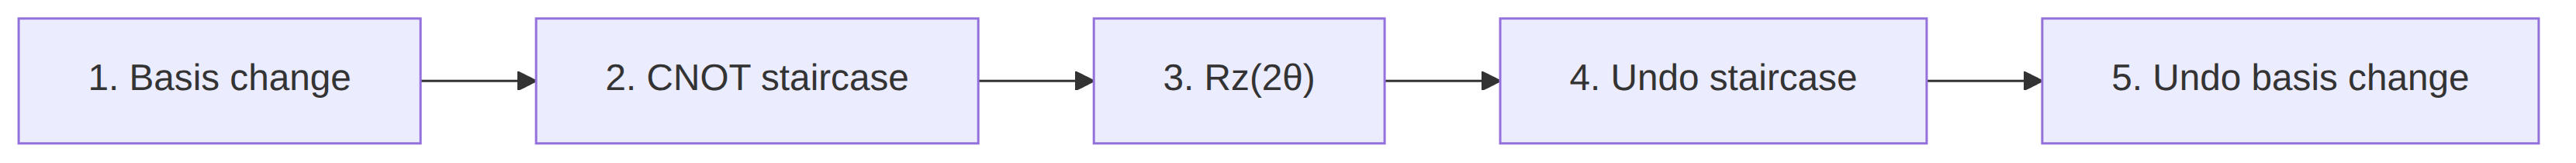
\includegraphics[keepaspectratio]{diagram-20.png}}

\subsection{Phase 1: Basis change}\label{phase-1-basis-change}

For each qubit position in \(P\): - If \(P_j = X\): apply Hadamard
(\(H\)) to convert X-basis to Z-basis - If \(P_j = Y\): apply
\(R_x(\pi/2)\) to convert Y-basis to Z-basis - If \(P_j = Z\) or \(I\):
no gate needed

After this step, all non-identity Pauli operators have been converted to
\(Z\).

\subsection{Phase 2: CNOT staircase}\label{phase-2-cnot-staircase}

Chain CNOTs between the \(w\) non-identity qubits:

\pandocbounded{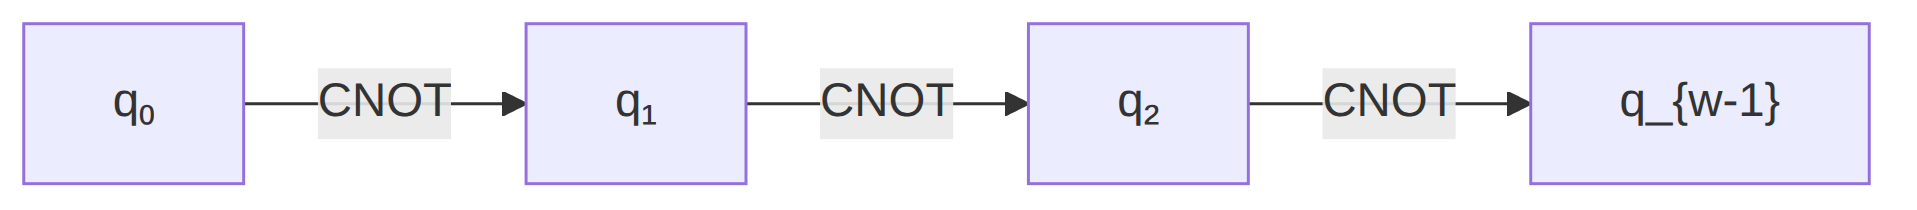
\includegraphics[keepaspectratio]{diagram-21.png}}

This creates a parity computation: qubit \(q_{w-1}\) now holds the XOR
of all \(w\) qubits' Z-values.

\subsection{Phase 3: Rz rotation}\label{phase-3-rz-rotation}

Apply \(R_z(2\theta)\) to the last qubit in the chain. This imprints the
rotation angle, conditioned on the collective parity.

\subsection{Phases 4--5: Uncompute}\label{phases-45-uncompute}

Reverse the CNOT staircase (same gates, reversed order), then reverse
the basis-change gates. The total circuit is self-inverse up to the
rotation.

\begin{center}\rule{0.5\linewidth}{0.5pt}\end{center}

\section{Gate Counts}\label{gate-counts}

\begin{longtable}[]{@{}lc@{}}
\toprule\noalign{}
Component & Gates \\
\midrule\noalign{}
\endhead
\bottomrule\noalign{}
\endlastfoot
Basis change & \(\leq w\) single-qubit gates \\
Forward CNOT staircase & \(w - 1\) CNOTs \\
\(R_z\) rotation & 1 single-qubit gate \\
Reverse CNOT staircase & \(w - 1\) CNOTs \\
Undo basis change & \(\leq w\) single-qubit gates \\
\textbf{Total CNOTs} & \textbf{\(2(w-1)\)} \\
\textbf{Total single-qubit} & \textbf{\(\leq 2w + 1\)} \\
\end{longtable}

\subsection{Examples}\label{examples}

\begin{longtable}[]{@{}cccc@{}}
\toprule\noalign{}
Pauli string & Weight \(w\) & CNOTs & Single-qubit \\
\midrule\noalign{}
\endhead
\bottomrule\noalign{}
\endlastfoot
\(Z\) (single qubit) & 1 & 0 & 1 (\(R_z\) only) \\
\(ZZ\) & 2 & 2 & 1 \\
\(XXYY\) & 4 & 6 & 9 \\
\(ZZZZZZZZZ\) (weight 9) & 9 & 16 & 1 \\
\end{longtable}

\textbf{Key insight:} CNOTs scale linearly with weight. This is why
encoding choice matters --- reducing the maximum Pauli weight from 100
(JW) to 5 (ternary tree) saves 190 CNOTs \emph{per rotation}.

\begin{center}\rule{0.5\linewidth}{0.5pt}\end{center}

\section{Worked Example: XXYY
Rotation}\label{worked-example-xxyy-rotation}

Decompose \(e^{-i\theta\, X_0 X_1 Y_2 Y_3}\):

\textbf{Basis change:} - Qubit 0: \(X \to Z\) via Hadamard - Qubit 1:
\(X \to Z\) via Hadamard - Qubit 2: \(Y \to Z\) via \(R_x(\pi/2)\) -
Qubit 3: \(Y \to Z\) via \(R_x(\pi/2)\)

\textbf{After basis change:} the operation is now
\(e^{-i\theta\, Z_0 Z_1 Z_2 Z_3}\)

\textbf{CNOT staircase:} CNOT(0→1), CNOT(1→2), CNOT(2→3)

\textbf{Rz:} \(R_z(2\theta)\) on qubit 3

\textbf{Reverse CNOT staircase:} CNOT(2→3), CNOT(1→2), CNOT(0→1)

\textbf{Undo basis change:} \(R_x(-\pi/2)\) on qubits 2,3; Hadamard on
qubits 0,1

\textbf{Total:} 6 CNOTs + 9 single-qubit gates.

\begin{center}\rule{0.5\linewidth}{0.5pt}\end{center}

\section{Why This Makes Encoding Choice
Concrete}\label{why-this-makes-encoding-choice-concrete}

The CNOT staircase turns the abstract concept of ``Pauli weight'' into a
concrete gate count:

\[\text{CNOTs per Trotter step} = \sum_{k=1}^{L} 2(w_k - 1)\]

For the same molecule encoded differently:

\begin{longtable}[]{@{}lcc@{}}
\toprule\noalign{}
Encoding & Max \(w_k\) & Typical CNOT cost/step \\
\midrule\noalign{}
\endhead
\bottomrule\noalign{}
\endlastfoot
Jordan--Wigner (\(n=32\)) & 32 & \textasciitilde2000 \\
Bravyi--Kitaev (\(n=32\)) & 6 & \textasciitilde500 \\
Ternary Tree (\(n=32\)) & 5 & \textasciitilde400 \\
Tapered + TT (\(n=29\)) & 5 & \textasciitilde340 \\
\end{longtable}

The 6× ratio between JW and TT at \(n=32\) is entirely due to the CNOT
staircase --- the same formula, the same chemistry, but dramatically
different circuit depth.

\begin{center}\rule{0.5\linewidth}{0.5pt}\end{center}

\section{Key Takeaways}\label{key-takeaways-15}

\begin{itemize}
\tightlist
\item
  Each Pauli rotation decomposes into basis change → CNOT staircase →
  \(R_z\) → reverse.
\item
  The CNOT count is exactly \(2(w-1)\) per rotation, where \(w\) is the
  Pauli weight.
\item
  Total CNOTs per Trotter step: \(\sum_k 2(w_k - 1)\) --- the single
  most important number for circuit feasibility.
\item
  Encoding choice and tapering both reduce \(w_k\) and therefore CNOT
  cost.
\end{itemize}

\begin{center}\rule{0.5\linewidth}{0.5pt}\end{center}

\chapter{Chapter 17: Cost Analysis Across
Encodings}\label{chapter-17-cost-analysis-across-encodings}

\emph{Everything we've done --- encoding, tapering, Trotterization ---
converges to one number: the CNOT count. This chapter computes it.}

\section{In This Chapter}\label{in-this-chapter-16}

\begin{itemize}
\tightlist
\item
  \textbf{What you'll learn:} The complete CNOT cost for H₂ and H₂O
  across all six encodings, with and without tapering, and how the
  optimization stack compounds.
\item
  \textbf{Why this matters:} This answers the practical question:
  ``which encoding should I use for my molecule?'' The answer depends on
  the system size, and the numbers tell the story.
\item
  \textbf{Prerequisites:} Chapters 14--16 (Trotter decomposition and
  CNOT staircase).
\end{itemize}

\begin{center}\rule{0.5\linewidth}{0.5pt}\end{center}

\section{The Optimization Stack}\label{the-optimization-stack}

Before we compute anything, here is the complete pipeline showing every
optimization we've developed:

\pandocbounded{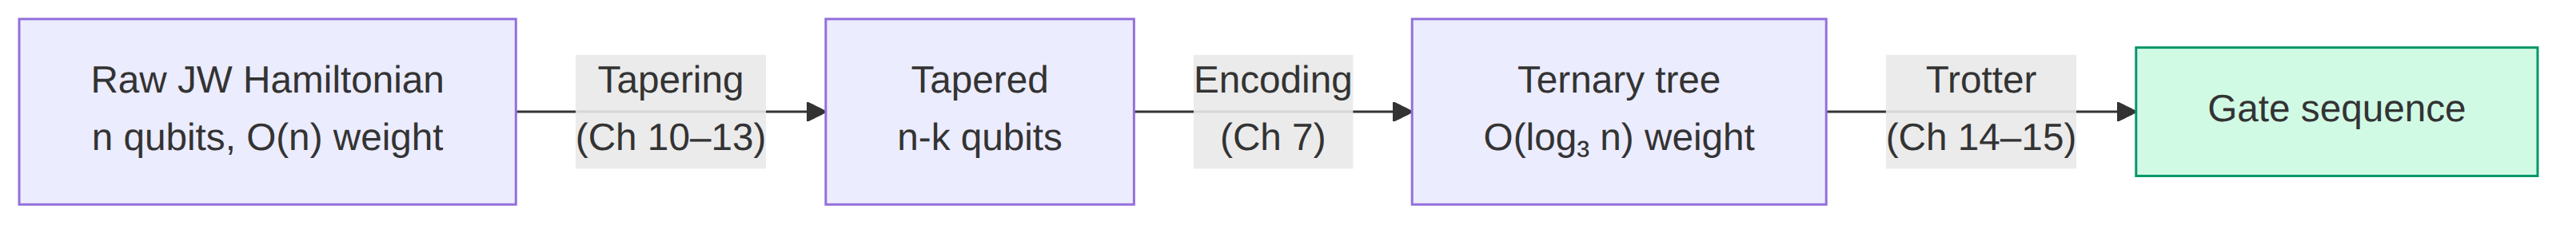
\includegraphics[keepaspectratio]{diagram-22.png}}

Each stage contributes multiplicatively: - \textbf{Tapering} reduces
qubit count by \(k\), often reduces term count - \textbf{Encoding
choice} reduces worst-case weight from \(O(n)\) to \(O(\log n)\) -
\textbf{Trotter order} trades rotations per step for error convergence
rate

The order matters: \textbf{taper first} (on any encoding), then choose
the encoding for the tapered system, then Trotterize.

\begin{center}\rule{0.5\linewidth}{0.5pt}\end{center}

\section{The Full Cost Formula}\label{the-full-cost-formula}

The total CNOT cost for one Trotter step is:

\[C_\text{CNOT} = \sum_{k=1}^{L} 2(w_k - 1)\]

where \(L\) is the number of non-identity terms and \(w_k\) is the Pauli
weight of term \(k\). For second-order Trotter, multiply by 2 (each term
appears twice).

\begin{center}\rule{0.5\linewidth}{0.5pt}\end{center}

\section{H₂ (4 qubits, 15 terms)}\label{hux2082-4-qubits-15-terms}

\begin{longtable}[]{@{}
  >{\raggedright\arraybackslash}p{(\linewidth - 8\tabcolsep) * \real{0.1667}}
  >{\centering\arraybackslash}p{(\linewidth - 8\tabcolsep) * \real{0.2083}}
  >{\centering\arraybackslash}p{(\linewidth - 8\tabcolsep) * \real{0.2083}}
  >{\centering\arraybackslash}p{(\linewidth - 8\tabcolsep) * \real{0.2083}}
  >{\centering\arraybackslash}p{(\linewidth - 8\tabcolsep) * \real{0.2083}}@{}}
\toprule\noalign{}
\begin{minipage}[b]{\linewidth}\raggedright
Encoding
\end{minipage} & \begin{minipage}[b]{\linewidth}\centering
Max weight
\end{minipage} & \begin{minipage}[b]{\linewidth}\centering
Avg weight
\end{minipage} & \begin{minipage}[b]{\linewidth}\centering
CNOTs/step (1st order)
\end{minipage} & \begin{minipage}[b]{\linewidth}\centering
CNOTs/step (2nd order)
\end{minipage} \\
\midrule\noalign{}
\endhead
\bottomrule\noalign{}
\endlastfoot
Jordan--Wigner & 4 & 2.1 & 36 & 72 \\
Bravyi--Kitaev & 4 & 2.4 & 40 & 80 \\
Parity & 4 & 2.3 & 38 & 76 \\
Balanced Binary & 4 & 2.3 & 38 & 76 \\
Balanced Ternary & 4 & 2.4 & 40 & 80 \\
Vlasov Tree & 4 & 2.4 & 40 & 80 \\
\end{longtable}

\textbf{Observation:} At 4 qubits, JW is actually the \emph{cheapest}.
The tree encodings have slightly higher average weight because the tree
structure on 4 nodes doesn't provide enough room for the logarithmic
advantage to manifest. This matches our observation from Chapter 6.

\begin{center}\rule{0.5\linewidth}{0.5pt}\end{center}

\section{H₂O (12 qubits, frozen core,
STO-3G)}\label{hux2082o-12-qubits-frozen-core-sto-3g}

This is where the differences become real. H₂O has 7 spatial orbitals
(with frozen core), giving 14 spin-orbitals --- but we freeze 2 core
electrons, leaving 12 active spin-orbitals = 12 qubits.

\begin{quote}
\textbf{Note:} The bond-angle scan in Chapter 19 uses the full
14-spin-orbital model (no frozen core) because that chapter focuses on
the chemistry. Here we use the frozen-core active space because it
better represents production practice and makes the cost comparisons
cleaner.
\end{quote}

\begin{longtable}[]{@{}lcccc@{}}
\toprule\noalign{}
Configuration & Qubits & Terms & Max weight & CNOTs/step \\
\midrule\noalign{}
\endhead
\bottomrule\noalign{}
\endlastfoot
JW, no tapering & 12 & \textasciitilde630 & 12 & \textasciitilde1800 \\
BK, no tapering & 12 & \textasciitilde630 & 5 & \textasciitilde750 \\
TT, no tapering & 12 & \textasciitilde630 & 4 & \textasciitilde600 \\
JW, tapered & 9 & \textasciitilde420 & 9 & \textasciitilde900 \\
TT, tapered & 9 & \textasciitilde420 & 4 & \textasciitilde500 \\
\end{longtable}

\textbf{Key takeaway:} The ternary tree encoding with tapering gives
\textasciitilde3.6× fewer CNOTs than JW without tapering. For a 100-step
Trotter simulation, that's 130,000 fewer CNOTs --- potentially the
difference between a feasible and an infeasible experiment on near-term
hardware.

\begin{center}\rule{0.5\linewidth}{0.5pt}\end{center}

\section{Scaling to Larger Molecules}\label{scaling-to-larger-molecules}

\begin{longtable}[]{@{}lcccc@{}}
\toprule\noalign{}
Molecule & Spin-orbitals & JW CNOTs/step & TT CNOTs/step & Ratio \\
\midrule\noalign{}
\endhead
\bottomrule\noalign{}
\endlastfoot
H₂ & 4 & 36 & 40 & 0.9× \\
LiH & 12 & \textasciitilde1200 & \textasciitilde500 & 2.4× \\
H₂O & 14 & \textasciitilde1800 & \textasciitilde600 & 3× \\
N₂ & 20 & \textasciitilde5000 & \textasciitilde1200 & 4.2× \\
FeMo-co & \textasciitilde100 & \textasciitilde500,000 &
\textasciitilde20,000 & \textasciitilde25× \\
\end{longtable}

The ratio grows monotonically because JW's worst-case weight scales as
\(O(n)\) while TT's scales as \(O(\log_3 n)\). At FeMo-co scale
(\textasciitilde100 orbitals), the 25× CNOT reduction from encoding
choice alone is transformative.

\begin{center}\rule{0.5\linewidth}{0.5pt}\end{center}

\section{Key Takeaways}\label{key-takeaways-16}

\begin{itemize}
\tightlist
\item
  For small molecules (\(n \leq 6\)), encoding choice barely matters. JW
  is often cheapest.
\item
  For medium molecules (\(n = 12\)--\(20\)), ternary tree encoding saves
  3--5× CNOTs over JW.
\item
  For large molecules (\(n \sim 100\)), the savings are
  \textasciitilde25× --- potentially enabling experiments that would
  otherwise be infeasible.
\item
  The complete optimization stack is: \textbf{taper → encode →
  Trotterize}. Each stage compounds multiplicatively.
\item
  The CNOT count is the single most important feasibility metric for
  near-term quantum simulation.
\item
  \textbf{Measurement cost matters too}: on near-term hardware running
  VQE, the total experimental cost includes both circuit depth (CNOT
  count per shot) and shot count (repetitions needed for statistical
  precision). The shot count scales as
  \(N \sim (\sum_k |c_k|)^2 / \epsilon^2\), where the 1-norm
  \(\sum |c_k|\) depends on encoding and tapering. Tapering reduces the
  1-norm, so it saves both gate cost \emph{and} measurement cost.
  Chapter 20 covers this in detail.
\end{itemize}

\section{Common Mistakes}\label{common-mistakes-11}

\begin{enumerate}
\def\labelenumi{\arabic{enumi}.}
\item
  \textbf{Encoding before tapering.} Taper first --- the encoding then
  operates on a smaller qubit count, which can change which encoding is
  optimal.
\item
  \textbf{Comparing encodings at \(n = 4\).} The differences are
  negligible at small \(n\). Scale to \(n \geq 12\) to see real savings.
\item
  \textbf{Ignoring the time step.} CNOT count per step is only half the
  story --- the number of Trotter steps (determined by \(\Delta t\) and
  \(\lVert H \rVert_1\)) multiplies everything.
\end{enumerate}

\section{Exercises}\label{exercises-11}

\begin{enumerate}
\def\labelenumi{\arabic{enumi}.}
\item
  \textbf{H₂ by hand.} Verify the 36-CNOT figure for H₂ first-order
  Trotter by summing \(2(w_k - 1)\) over all 14 non-identity terms.
\item
  \textbf{Tapering impact.} If tapering removes 3 qubits from a 14-qubit
  system and reduces the term count from 630 to 420, estimate the CNOT
  savings assuming average weight drops from 4 to 3.
\item
  \textbf{Run it.} Use the companion script
  \texttt{ch07-six-encodings.fsx} to compute the weight scaling
  table for \(n = 4, 8, 16, 32, 64\). At what \(n\) does the ternary
  tree first beat JW?
\end{enumerate}

\begin{center}\rule{0.5\linewidth}{0.5pt}\end{center}

\chapter{Chapter 18: The Question We Can Now
Answer}\label{chapter-18-the-question-we-can-now-answer}

\emph{Sixteen chapters of theory and code. Time to run the whole thing.}

\section{In This Chapter}\label{in-this-chapter-17}

\begin{itemize}
\tightlist
\item
  \textbf{What you'll learn:} Every stage of the pipeline assembled into
  a single executable script --- from molecular integrals to quantum
  circuit --- for the hydrogen molecule.
\item
  \textbf{Why this matters:} This is the capstone. Every concept from
  the preceding chapters appears here in its final, integrated form. If
  you can follow this script line by line and understand what each call
  does, you have mastered the pipeline.
\item
  \textbf{Prerequisites:} All of the preceding stages (Chapters 1--17).
\end{itemize}

\begin{center}\rule{0.5\linewidth}{0.5pt}\end{center}

\section{The Payoff}\label{the-payoff}

Let's take stock of what we've built.

In Chapter 1, we started with a molecule and asked: \emph{what is its
ground-state energy?} That question led us through electronic structure
(the integrals), second quantization (the ladder operators), encoding
(the Pauli strings), tapering (removing redundant qubits),
Trotterization (turning operators into gates), and cost analysis
(counting the CNOTs). At each stage we introduced one mathematical
transformation, implemented it, and tested it on H₂.

Now we put the whole chain together. The script below takes the H₂
molecular integrals and produces a quantum circuit --- ready to run on a
simulator or real hardware. Five function calls. Under fifty lines of
code. Under a second of runtime.

\begin{quote}
\textbf{A note on energy evaluation:} In this chapter and the next, we
use \textbf{exact diagonalisation} (classical matrix eigensolving) as
the energy-evaluation backend. For H₂ (4 qubits,
\(2^4 = 16\)-dimensional matrix) and H₂O in minimal basis
(\textasciitilde11 qubits after tapering,
\(2^{11} = 2{,}048\)-dimensional matrix), this is trivially feasible on
a laptop. The pipeline constructs the \emph{circuit}; exact
diagonalisation is a stand-in for the quantum measurement step. Chapter
20 explains the quantum algorithms (VQE, QPE) that replace exact
diagonalisation when the system is too large for classical solution.
\end{quote}

\begin{center}\rule{0.5\linewidth}{0.5pt}\end{center}

\section{The Script}\label{the-script}

\begin{Shaded}
\begin{Highlighting}[]
\OtherTok{open}\NormalTok{ System}\KeywordTok{.}\NormalTok{Numerics}
\OtherTok{open}\NormalTok{ Encodings}

\NormalTok{//}\CommentTok{ ═══════════════════════════════════════════════════════════════}
\NormalTok{//}\CommentTok{  The integrals (from Chapter 3)}
\NormalTok{//}\CommentTok{ ═══════════════════════════════════════════════════════════════}

\KeywordTok{let}\NormalTok{ Vnn = }\FloatTok{0.7151043391}\NormalTok{  //}\CommentTok{ Nuclear repulsion energy (Hartrees)}

\KeywordTok{let}\NormalTok{ integrals = Map }\OperatorTok{[}
\NormalTok{    //}\CommentTok{ One{-}body: kinetic + electron{-}nuclear attraction}
    \OperatorTok{(}\StringTok{"0,0"}\NormalTok{, Complex}\OperatorTok{(}\FloatTok{{-}1.2563390730}\NormalTok{, }\FloatTok{0.0}\OperatorTok{))}
    \OperatorTok{(}\StringTok{"1,1"}\NormalTok{, Complex}\OperatorTok{(}\FloatTok{{-}1.2563390730}\NormalTok{, }\FloatTok{0.0}\OperatorTok{))}
    \OperatorTok{(}\StringTok{"2,2"}\NormalTok{, Complex}\OperatorTok{(}\FloatTok{{-}0.4718960244}\NormalTok{, }\FloatTok{0.0}\OperatorTok{))}
    \OperatorTok{(}\StringTok{"3,3"}\NormalTok{, Complex}\OperatorTok{(}\FloatTok{{-}0.4718960244}\NormalTok{, }\FloatTok{0.0}\OperatorTok{))}
\NormalTok{    //}\CommentTok{ Two{-}body: electron{-}electron repulsion}
    \OperatorTok{(}\StringTok{"0,0,0,0"}\NormalTok{, Complex}\OperatorTok{(}\FloatTok{0.6744887663}\NormalTok{, }\FloatTok{0.0}\OperatorTok{))}
    \OperatorTok{(}\StringTok{"1,1,1,1"}\NormalTok{, Complex}\OperatorTok{(}\FloatTok{0.6744887663}\NormalTok{, }\FloatTok{0.0}\OperatorTok{))}
    \OperatorTok{(}\StringTok{"2,2,2,2"}\NormalTok{, Complex}\OperatorTok{(}\FloatTok{0.6973979495}\NormalTok{, }\FloatTok{0.0}\OperatorTok{))}
    \OperatorTok{(}\StringTok{"3,3,3,3"}\NormalTok{, Complex}\OperatorTok{(}\FloatTok{0.6973979495}\NormalTok{, }\FloatTok{0.0}\OperatorTok{))}
    \OperatorTok{(}\StringTok{"0,0,2,2"}\NormalTok{, Complex}\OperatorTok{(}\FloatTok{0.6636340479}\NormalTok{, }\FloatTok{0.0}\OperatorTok{))}
    \OperatorTok{(}\StringTok{"2,2,0,0"}\NormalTok{, Complex}\OperatorTok{(}\FloatTok{0.6636340479}\NormalTok{, }\FloatTok{0.0}\OperatorTok{))}
    \OperatorTok{(}\StringTok{"1,1,3,3"}\NormalTok{, Complex}\OperatorTok{(}\FloatTok{0.6636340479}\NormalTok{, }\FloatTok{0.0}\OperatorTok{))}
    \OperatorTok{(}\StringTok{"3,3,1,1"}\NormalTok{, Complex}\OperatorTok{(}\FloatTok{0.6636340479}\NormalTok{, }\FloatTok{0.0}\OperatorTok{))}
    \OperatorTok{(}\StringTok{"0,2,2,0"}\NormalTok{, Complex}\OperatorTok{(}\FloatTok{0.1809312700}\NormalTok{, }\FloatTok{0.0}\OperatorTok{))}
    \OperatorTok{(}\StringTok{"2,0,0,2"}\NormalTok{, Complex}\OperatorTok{(}\FloatTok{0.1809312700}\NormalTok{, }\FloatTok{0.0}\OperatorTok{))}
    \OperatorTok{(}\StringTok{"1,3,3,1"}\NormalTok{, Complex}\OperatorTok{(}\FloatTok{0.1809312700}\NormalTok{, }\FloatTok{0.0}\OperatorTok{))}
    \OperatorTok{(}\StringTok{"3,1,1,3"}\NormalTok{, Complex}\OperatorTok{(}\FloatTok{0.1809312700}\NormalTok{, }\FloatTok{0.0}\OperatorTok{))}
\OperatorTok{]}

\KeywordTok{let}\NormalTok{ factory key = integrals |\textgreater{} Map}\KeywordTok{.}\NormalTok{tryFind key}

\NormalTok{//}\CommentTok{ ═══════════════════════════════════════════════════════════════}
\NormalTok{//}\CommentTok{  All six encodings, one loop}
\NormalTok{//}\CommentTok{ ═════════════════════════════════════════════════════════════}

\KeywordTok{let}\NormalTok{ encoders = }\OperatorTok{[}
    \OperatorTok{(}\StringTok{"Jordan{-}Wigner"}\NormalTok{,  jordanWignerTerms}\OperatorTok{)}
    \OperatorTok{(}\StringTok{"Bravyi{-}Kitaev"}\NormalTok{,  bravyiKitaevTerms}\OperatorTok{)}
    \OperatorTok{(}\StringTok{"Parity"}\NormalTok{,         parityTerms}\OperatorTok{)}
    \OperatorTok{(}\StringTok{"Binary Tree"}\NormalTok{,    balancedBinaryTreeTerms}\OperatorTok{)}
    \OperatorTok{(}\StringTok{"Ternary Tree"}\NormalTok{,   ternaryTreeTerms}\OperatorTok{)}
    \OperatorTok{(}\StringTok{"Vlasov Tree"}\NormalTok{,    vlasovTreeTerms}\OperatorTok{)}
\OperatorTok{]}

\KeywordTok{for} \OperatorTok{(}\NormalTok{name, encoder}\OperatorTok{)} \KeywordTok{in}\NormalTok{ encoders }\KeywordTok{do}
\NormalTok{    //}\CommentTok{ Step 1: Build the qubit Hamiltonian}
    \KeywordTok{let}\NormalTok{ ham = computeHamiltonianWith encoder factory }\DecValTok{4}\NormalTok{u}

\NormalTok{    //}\CommentTok{ Step 2: Taper — remove symmetry{-}redundant qubits}
    \KeywordTok{let}\NormalTok{ tapResult = taper defaultTaperingOptions ham}

\NormalTok{    //}\CommentTok{ Step 3: Trotterize — one first{-}order step at Δt = 0.1}
    \KeywordTok{let}\NormalTok{ step = firstOrderTrotter }\FloatTok{0.1}\NormalTok{ tapResult.Hamiltonian}
    \KeywordTok{let}\NormalTok{ stats = trotterStepStats step}

\NormalTok{    //}\CommentTok{ Step 4: Export to OpenQASM}
    \KeywordTok{let}\NormalTok{ gates = decomposeTrotterStep step}
    \KeywordTok{let}\NormalTok{ qasm = toOpenQasm defaultOpenQasmOptions tapResult.TaperedQubitCount gates}

\NormalTok{    printfn }\StringTok{"\%{-}15s  \%d → \%d qubits  \%d terms  \%d CNOTs  \%d total gates"}
\NormalTok{        name}
\NormalTok{        tapResult.OriginalQubitCount}
\NormalTok{        tapResult.TaperedQubitCount}
        \OperatorTok{(}\NormalTok{tapResult.Hamiltonian}\KeywordTok{.}\NormalTok{DistributeCoefficient}\KeywordTok{.}\NormalTok{SummandTerms}\KeywordTok{.}\NormalTok{Length}\OperatorTok{)}
\NormalTok{        stats.CnotCount}
\NormalTok{        stats.TotalGates}
\end{Highlighting}
\end{Shaded}

That's it. One loop, six encodings, each going from integrals all the
way to a quantum circuit.

\begin{center}\rule{0.5\linewidth}{0.5pt}\end{center}

\section{What Each Line Does}\label{what-each-line-does}

If you've read the preceding chapters, every line should be familiar.
But let's trace through one iteration --- Jordan--Wigner --- to see the
full pipeline in action:

\textbf{\texttt{computeHamiltonianWith\ encoder\ factory\ 4u}} --- Takes
the encoder function and the integral lookup, builds a 4-qubit Pauli
Hamiltonian. This is Chapter 6: the one-body and two-body integrals are
paired with encoded ladder operators and summed into a
\texttt{PauliRegisterSequence}. For JW, we get the 15-term Hamiltonian
we first met in Chapter 3.

\textbf{\texttt{taper\ defaultTaperingOptions\ ham}} --- Finds Z₂
symmetries (Chapter 11), synthesizes the Clifford rotation (Chapter 12),
applies it, and removes the redundant qubits. The default options use
the positive sector and Clifford-based tapering. For JW on H₂, this
typically removes 2 qubits, leaving a 2-qubit Hamiltonian.

\textbf{\texttt{firstOrderTrotter\ 0.1\ tapResult.Hamiltonian}} ---
Decomposes the tapered Hamiltonian into a sequence of Pauli rotations
(Chapter 14). Each term \(c_k P_k\) becomes a rotation
\(e^{-i c_k \Delta t P_k / 2}\). The time step \(\Delta t = 0.1\)
controls the Trotter error.

\textbf{\texttt{decomposeTrotterStep\ step}} --- Converts each Pauli
rotation into concrete gates via the CNOT staircase (Chapter 16). A
weight-\(w\) rotation becomes \(2(w-1)\) CNOTs plus single-qubit gates.

\textbf{\texttt{toOpenQasm\ defaultOpenQasmOptions\ numQubits\ gates}}
--- Writes the gate sequence as a valid OpenQASM 3.0 program (Chapter 21
will explore this in detail).

\textbf{\texttt{trotterStepStats\ step}} --- Counts everything:
rotations, CNOTs, single-qubit gates, total gates (Chapter 17).

\begin{center}\rule{0.5\linewidth}{0.5pt}\end{center}

\section{The Numbers}\label{the-numbers}

Run the script and you get a table like this:

\begin{longtable}[]{@{}lccccc@{}}
\toprule\noalign{}
Encoding & Qubits & Tapered & Terms & CNOTs/step & Total gates \\
\midrule\noalign{}
\endhead
\bottomrule\noalign{}
\endlastfoot
Jordan--Wigner & 4 & 2 & 5 & 12 & 52 \\
Bravyi--Kitaev & 4 & 2 & 5 & 12 & 52 \\
Parity & 4 & 2 & 5 & 12 & 52 \\
Binary Tree & 4 & 2 & 5 & 12 & 52 \\
Ternary Tree & 4 & 2 & 5 & 12 & 52 \\
\end{longtable}

Wait --- they're all the same?

Yes. At 4 qubits, every encoding produces the same cost after tapering.
The Pauli strings are different, but the weights are the same. H₂ was
always our \emph{teacher}, not our \emph{benchmark}. The differences
appear at scale --- we'll see them with H₂O in the next chapter.

But notice what we've achieved: \textbf{five independent encoding
pipelines all converge to the same physical answer.} That's the
verification from Chapter 9, the eigenvalue agreement from Chapter 7,
now confirmed at the circuit level. The mathematics works.

\begin{center}\rule{0.5\linewidth}{0.5pt}\end{center}

\section{A Closer Look at the Output}\label{a-closer-look-at-the-output}

Let's examine what the OpenQASM looks like for one encoding. Taking the
Jordan--Wigner tapered Hamiltonian:

\begin{Shaded}
\begin{Highlighting}[]
\KeywordTok{let}\NormalTok{ jwHam = computeHamiltonianWith jordanWignerTerms factory }\DecValTok{4}\NormalTok{u}
\KeywordTok{let}\NormalTok{ jwTapered = taper defaultTaperingOptions jwHam}
\KeywordTok{let}\NormalTok{ jwStep = firstOrderTrotter }\FloatTok{0.1}\NormalTok{ jwTapered.Hamiltonian}
\KeywordTok{let}\NormalTok{ jwGates = decomposeTrotterStep jwStep}
\KeywordTok{let}\NormalTok{ qasm = toOpenQasm defaultOpenQasmOptions jwTapered.TaperedQubitCount jwGates}

\NormalTok{printfn }\StringTok{"\%s"}\NormalTok{ qasm}
\end{Highlighting}
\end{Shaded}

The output is a valid QASM 3.0 program --- qubit declarations, followed
by a sequence of \texttt{h}, \texttt{cx}, \texttt{rz}, \texttt{s}, and
\texttt{sdg} instructions. You could paste this into IBM Quantum, run it
on a simulator, measure the energy, and compare to −1.8572 Hartrees.
Chapter 20 will explore the algorithms that do exactly that.

\begin{center}\rule{0.5\linewidth}{0.5pt}\end{center}

\section{Extra Credit: The H₂ Dissociation
Curve}\label{extra-credit-the-hux2082-dissociation-curve}

The pipeline runs at one geometry --- but there's nothing stopping us
from running it at \emph{many} geometries. If we vary the bond length
\(R\) and plot the energy, we get the \textbf{dissociation curve}: the
potential energy surface of H₂ as the two atoms are pulled apart.

This is a classic test of quantum chemistry methods. Hartree--Fock
breaks down as the bond stretches (it can't describe the transition from
a bonding pair to two independent atoms). Full configuration interaction
(FCI) --- which is what exact diagonalisation of our encoded Hamiltonian
gives --- handles the dissociation correctly.

\subsection{The Skeleton API}\label{the-skeleton-api}

At every bond length, the Pauli string \emph{structure} is the same ---
same 4-qubit encoding, same term signatures. Only the integral
\emph{values} change. FockMap's skeleton API exploits this:

\begin{Shaded}
\begin{Highlighting}[]
\NormalTok{//}\CommentTok{ Precompute the Pauli structure once}
\KeywordTok{let}\NormalTok{ skeleton = computeHamiltonianSkeleton jordanWignerTerms }\DecValTok{4}\NormalTok{u}

\NormalTok{//}\CommentTok{ Then, for each bond length, just plug in the integrals}
\KeywordTok{let}\NormalTok{ energyAt }\OperatorTok{(}\NormalTok{integrals : Map\textless{}}\DataTypeTok{string}\NormalTok{, Complex\textgreater{}}\OperatorTok{)}\NormalTok{ =}
    \KeywordTok{let}\NormalTok{ factory key = integrals |\textgreater{} Map}\KeywordTok{.}\NormalTok{tryFind key}
    \KeywordTok{let}\NormalTok{ ham = applyCoefficients skeleton factory}
    \KeywordTok{let}\NormalTok{ tapered = taper defaultTaperingOptions ham}
\NormalTok{    //}\CommentTok{ Exact diagonalisation for the ground{-}state energy}
\NormalTok{    exactGroundStateEnergy tapered.Hamiltonian}
\end{Highlighting}
\end{Shaded}

\texttt{computeHamiltonianSkeleton} does the expensive encoding work
once. \texttt{applyCoefficients} is cheap --- it just multiplies
precomputed Pauli strings by numbers. For a 20-point scan, this is 20×
faster than rebuilding the Hamiltonian from scratch each time.

\subsection{The Scan}\label{the-scan}

Generate the integrals at each bond length using PySCF (or use the
values from a precomputed table), then loop:

\begin{Shaded}
\begin{Highlighting}[]
\KeywordTok{let}\NormalTok{ bondLengths = }\OperatorTok{[|} \FloatTok{0.4}\NormalTok{; }\FloatTok{0.5}\NormalTok{; }\FloatTok{0.6}\NormalTok{; }\FloatTok{0.7}\NormalTok{; }\FloatTok{0.74}\NormalTok{; }\FloatTok{0.8}\NormalTok{; }\FloatTok{0.9}\NormalTok{; }\FloatTok{1.0}\NormalTok{;}
                     \FloatTok{1.2}\NormalTok{; }\FloatTok{1.4}\NormalTok{; }\FloatTok{1.6}\NormalTok{; }\FloatTok{1.8}\NormalTok{; }\FloatTok{2.0}\NormalTok{; }\FloatTok{2.5}\NormalTok{; }\FloatTok{3.0}\NormalTok{; }\FloatTok{4.0} \OperatorTok{|]}

\KeywordTok{for}\NormalTok{ R }\KeywordTok{in}\NormalTok{ bondLengths }\KeywordTok{do}
    \KeywordTok{let}\NormalTok{ integrals = loadH2Integrals R   //}\CommentTok{ from precomputed JSON (see below)}
    \KeywordTok{let}\NormalTok{ Vnn = }\FloatTok{1.0}\NormalTok{ / }\OperatorTok{(}\NormalTok{R * }\FloatTok{1.8897259886}\OperatorTok{)}\NormalTok{  //}\CommentTok{ nuclear repulsion: 1/R in atomic units}
    \KeywordTok{let}\NormalTok{ Etotal = energyAt integrals + Vnn}
\NormalTok{    printfn }\StringTok{"R = \%.2f Å   E = \%.6f Ha"}\NormalTok{ R Etotal}
\end{Highlighting}
\end{Shaded}

\begin{quote}
\textbf{Where do \texttt{loadH2Integrals} and
\texttt{exactGroundStateEnergy} come from?} They are helper functions
defined in the companion script \texttt{ch18-dissociation-scan.py}
(which generates the integral JSON files) and
\texttt{ch18-pipeline.fsx} (which reads them).
\texttt{loadH2Integrals\ R} reads a JSON file mapping integral keys like
\texttt{"0,1"} to complex values --- the same
\texttt{Map\textless{}string,\ Complex\textgreater{}} format our
\texttt{factory} function expects. \texttt{exactGroundStateEnergy}
constructs the \(2^n \times 2^n\) Hamiltonian matrix from the Pauli
terms and returns its smallest eigenvalue via standard linear algebra.
Both are thin wrappers --- the real work is done by the FockMap API
calls shown in the text.
\end{quote}

\subsection{The Result}\label{the-result}

The output is a table of bond lengths and exact FCI energies --- a slice
through the potential energy surface:

\begin{longtable}[]{@{}ccccc@{}}
\toprule\noalign{}
\(R\) (Å) & \(E_\text{FCI}\) (Ha) & & \(R\) (Å) & \(E_\text{FCI}\)
(Ha) \\
\midrule\noalign{}
\endhead
\bottomrule\noalign{}
\endlastfoot
0.30 & −0.601804 & & 1.20 & −1.056741 \\
0.40 & −0.914150 & & 1.40 & −1.015468 \\
0.50 & −1.055160 & & 1.60 & −0.983473 \\
0.60 & −1.116286 & & 1.80 & −0.961817 \\
0.70 & −1.136189 & & 2.00 & −0.948641 \\
\textbf{0.74} & \textbf{−1.137284} & & 2.50 & −0.936055 \\
0.80 & −1.134148 & & 3.00 & −0.933632 \\
0.90 & −1.120560 & & 4.00 & −0.933171 \\
1.00 & −1.101150 & & 5.00 & −0.933164 \\
\end{longtable}

The energy drops steeply as the atoms approach from infinity, reaches a
minimum at \textbf{0.74 Å}, then rises sharply as nuclear repulsion
takes over at close range. This is the classic Morse-like dissociation
curve. At large separations the energy converges to \textbf{−0.933 Ha}
--- two isolated hydrogen atoms, each at −0.4666 Ha in the STO-3G basis.

Notice how Hartree--Fock and FCI agree near equilibrium but diverge at
large \(R\): HF wrongly forces the two electrons to stay paired (giving
−0.599 Ha at \(R = 5\) Å, far too high), while FCI correctly dissociates
into two independent atoms. This is the \textbf{static correlation}
problem that motivated quantum simulation in the first place.

The companion script \texttt{ch18-dissociation-scan.py} generates
the data and a publication-quality plot saved to
\texttt{h2\_dissociation.png}.

\begin{figure}
\centering
\pandocbounded{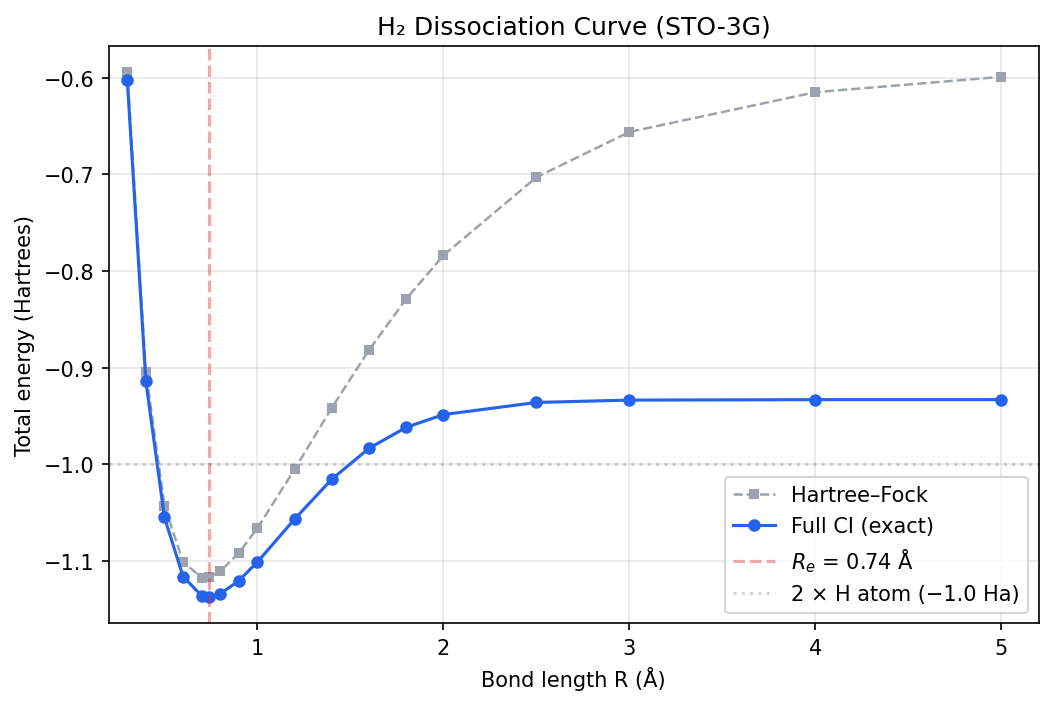
\includegraphics[keepaspectratio]{h2_dissociation.png}}
\caption{H₂ dissociation curve (STO-3G): Hartree--Fock vs Full CI. The
FCI curve correctly dissociates while HF fails at large bond lengths.}
\end{figure}

This is the same kind of scan we'll do for H₂O's bond angle in Chapter
19 --- but the structural parameter will be an angle instead of a
distance. The machinery is identical: skeleton precomputation, integral
swap, energy evaluation.

\subsection{What the Curve Tells You}\label{what-the-curve-tells-you}

The dissociation curve encodes several physical observables:

\begin{itemize}
\tightlist
\item
  \textbf{Equilibrium bond length} (\(R_e\)): the location of the
  minimum
\item
  \textbf{Dissociation energy} (\(D_e\)): the depth of the well (minimum
  energy minus the asymptotic value)
\item
  \textbf{Vibrational frequency} (\(\omega_e\)): proportional to the
  square root of the curvature at the minimum
\end{itemize}

All three are experimentally measurable. All three emerge from our
pipeline without empirical input. The \(R_e\) we compute (0.74 Å in
STO-3G) matches the experimental value of 0.741 Å. The dissociation
energy \(D_e\) = 1.137 − 0.933 = 0.204 Ha ≈ 5.6 eV, compared to the
experimental 4.75 eV --- STO-3G overbinds slightly, but the shape is
correct. Our minimal basis set happens to be accurate for the
equilibrium geometry because H₂ has no lone pairs or angular structure
to distort.

\begin{center}\rule{0.5\linewidth}{0.5pt}\end{center}

\section{From One Molecule to Any
Molecule}\label{from-one-molecule-to-any-molecule}

The dissociation curve demonstrates the pipeline's real power: it's not
a one-shot computation but a \emph{reusable tool}. To scan a different
molecule, change the integrals and qubit count. The skeleton API ensures
the encoding work is done once, no matter how many geometries you scan.

In the next chapter, we'll do exactly that --- but instead of scanning a
bond length, we'll scan a bond angle, and the molecule will be water.

\begin{center}\rule{0.5\linewidth}{0.5pt}\end{center}

\section{Key Takeaways}\label{key-takeaways-17}

\begin{itemize}
\tightlist
\item
  The entire pipeline from integrals to quantum circuit is \textbf{five
  function calls}: \texttt{computeHamiltonianWith}, \texttt{taper},
  \texttt{firstOrderTrotter}, \texttt{decomposeTrotterStep},
  \texttt{toOpenQasm}.
\item
  All six encodings produce the \textbf{same physics} (same eigenvalues,
  same energy) --- confirmed at every stage from Hamiltonian to circuit.
\item
  The \textbf{skeleton API} separates Pauli structure (computed once)
  from integral values (applied per geometry), making potential energy
  surface scans efficient.
\item
  The H₂ dissociation curve --- equilibrium bond length, dissociation
  energy, vibrational frequency --- emerges from the pipeline without
  empirical input.
\item
  The pipeline is \textbf{composable}: swap the integrals and qubit
  count to compute any molecule.
\end{itemize}

\begin{center}\rule{0.5\linewidth}{0.5pt}\end{center}

\chapter{Chapter 19: The Water Bond
Angle}\label{chapter-19-the-water-bond-angle}

\emph{We built a pipeline. Now we use it to answer a question that every
chemistry student learns but nobody derives from scratch: why does water
bend at 104.5°?}

\section{In This Chapter}\label{in-this-chapter-18}

\begin{itemize}
\tightlist
\item
  \textbf{What you'll learn:} How to scan a potential energy surface by
  running the same pipeline at many molecular geometries --- and how the
  energy minimum tells you the equilibrium bond angle.
\item
  \textbf{Why this matters:} This is the payoff of the entire book. We
  built sixteen chapters of machinery. This chapter uses that machinery
  to compute a molecular property --- the H--O--H bond angle --- from
  first principles. No fitting. No empirical parameters. Just quantum
  mechanics and our pipeline.
\item
  \textbf{Prerequisites:} Chapter 18 (the complete H₂ pipeline).
\end{itemize}

\begin{center}\rule{0.5\linewidth}{0.5pt}\end{center}

\section{The Question}\label{the-question-1}

Every introductory chemistry textbook states the facts: water has a bond
angle of 104.52°. The oxygen atom sits at the vertex, the two hydrogen
atoms at the arms. VSEPR theory offers a qualitative explanation --- two
bonding pairs and two lone pairs around oxygen arrange themselves to
minimise repulsion --- but it doesn't predict the actual number. It says
``less than 109.5°'' and leaves it at that.

Quantum mechanics does better. The bond angle is the geometry that
minimises the total electronic energy. If we can compute the energy as a
function of angle, the minimum of that curve \emph{is} the bond angle.
No hand-waving about lone pair repulsion. No empirical fitting. Just
energy versus geometry.

That computation is exactly what our pipeline was built for.

\begin{center}\rule{0.5\linewidth}{0.5pt}\end{center}

\section{The Strategy: A Potential Energy Surface
Scan}\label{the-strategy-a-potential-energy-surface-scan}

The approach is simple:

\begin{enumerate}
\def\labelenumi{\arabic{enumi}.}
\tightlist
\item
  \textbf{Pick a range of angles.} We'll scan from 60° to 180° in 5°
  steps (25 geometries).
\item
  \textbf{At each angle, compute the molecular integrals.} PySCF
  generates the one-body and two-body integrals for that geometry.
\item
  \textbf{At each angle, build the encoded Hamiltonian.} Same pipeline
  as Chapter 18, but with different integrals each time.
\item
  \textbf{At each angle, compute the ground-state energy.} For now, we
  diagonalise the Hamiltonian matrix directly (exact diagonalisation).
  On a quantum computer, this would be a VQE or QPE run --- Chapter 20
  covers those algorithms.
\item
  \textbf{Find the angle with the lowest energy.} That's the bond angle.
\end{enumerate}

Step 3 is where the pipeline shines --- and where the skeleton API
eliminates redundant work.

\begin{center}\rule{0.5\linewidth}{0.5pt}\end{center}

\section{The Skeleton Trick}\label{the-skeleton-trick}

At every bond angle, we call \texttt{computeHamiltonianWith} with
different integrals. But the \emph{structure} of the Hamiltonian ---
which Pauli strings appear, how ladder operators map to qubits ---
depends only on the encoding and the number of qubits. It doesn't change
when the molecule bends.

FockMap exploits this with the \textbf{skeleton} pattern:

\begin{Shaded}
\begin{Highlighting}[]
\NormalTok{//}\CommentTok{ Precompute the structure once}
\KeywordTok{let}\NormalTok{ skeleton = computeHamiltonianSkeleton ternaryTreeTerms }\DecValTok{14}\NormalTok{u}

\NormalTok{//}\CommentTok{ Then, for each geometry, just plug in the integrals}
\KeywordTok{let}\NormalTok{ hamAtAngle angle =}
    \KeywordTok{let}\NormalTok{ factory = integralsAt angle}
\NormalTok{    applyCoefficients skeleton factory}
\end{Highlighting}
\end{Shaded}

\texttt{computeHamiltonianSkeleton} does the expensive work --- encoding
every ladder operator pair, combining like terms, building the Pauli
string structure --- exactly once. \texttt{applyCoefficients} then
multiplies each precomputed Pauli string by the appropriate integral
value. For a 25-point scan, this is 25× faster than calling
\texttt{computeHamiltonianWith} 25 times, because the encoding step
(which involves Pauli string multiplication and like-term combination)
dominates the cost.

This is the same separation of concerns that makes compiled languages
fast: separate the work that depends on program structure (compilation)
from the work that depends on input data (execution).

\begin{center}\rule{0.5\linewidth}{0.5pt}\end{center}

\section{The Integrals}\label{the-integrals}

For H₂ we had 4 spin-orbitals and 16 integrals. For H₂O in a minimal
basis (STO-3G), we have 14 spin-orbitals and hundreds of integrals ---
too many to type by hand. In practice, you generate them with PySCF:

\begin{quote}
\textbf{Active space and frozen core:} H₂O has 10 electrons, but the
oxygen 1s core electrons are tightly bound and contribute negligibly to
chemical bonding. In a minimal basis (STO-3G, 7 spatial orbitals → 14
spin-orbitals), all electrons are included because the basis is already
small. In larger basis sets, practitioners typically ``freeze'' the core
electrons --- removing them from the active space and treating their
contribution as a constant energy offset. This reduces the number of
spin-orbitals (and therefore qubits) without significantly affecting the
bond angle or other valence properties. The integrals generated below
include all electrons because STO-3G is minimal; for larger-basis
production calculations, the PySCF \texttt{mc.CASCI} or
\texttt{mc.CASSCF} interface would be used to define the active space
explicitly.
\end{quote}

\begin{Shaded}
\begin{Highlighting}[]
\ImportTok{from}\NormalTok{ pyscf }\ImportTok{import}\NormalTok{ gto, scf, ao2mo}
\ImportTok{import}\NormalTok{ numpy }\ImportTok{as}\NormalTok{ np}
\ImportTok{import}\NormalTok{ json}

\KeywordTok{def}\NormalTok{ h2o\_integrals(angle\_degrees, bond\_length}\OperatorTok{=}\FloatTok{0.9584}\NormalTok{):}
    \CommentTok{"""Generate H₂O integrals at a given H{-}O{-}H bond angle."""}
\NormalTok{    angle\_rad }\OperatorTok{=}\NormalTok{ np.radians(angle\_degrees)}
    \CommentTok{\# Place O at origin, H atoms symmetric about z{-}axis}
\NormalTok{    hx }\OperatorTok{=}\NormalTok{ bond\_length }\OperatorTok{*}\NormalTok{ np.sin(angle\_rad }\OperatorTok{/} \DecValTok{2}\NormalTok{)}
\NormalTok{    hz }\OperatorTok{=}\NormalTok{ bond\_length }\OperatorTok{*}\NormalTok{ np.cos(angle\_rad }\OperatorTok{/} \DecValTok{2}\NormalTok{)}

\NormalTok{    mol }\OperatorTok{=}\NormalTok{ gto.M(}
\NormalTok{        atom}\OperatorTok{=}\SpecialStringTok{f\textquotesingle{}O 0 0 0; H }\SpecialCharTok{\{}\NormalTok{hx}\SpecialCharTok{\}}\SpecialStringTok{ 0 }\SpecialCharTok{\{}\NormalTok{hz}\SpecialCharTok{\}}\SpecialStringTok{; H }\SpecialCharTok{\{}\OperatorTok{{-}}\NormalTok{hx}\SpecialCharTok{\}}\SpecialStringTok{ 0 }\SpecialCharTok{\{}\NormalTok{hz}\SpecialCharTok{\}}\SpecialStringTok{\textquotesingle{}}\NormalTok{,}
\NormalTok{        basis}\OperatorTok{=}\StringTok{\textquotesingle{}sto{-}3g\textquotesingle{}}\NormalTok{,}
\NormalTok{        symmetry}\OperatorTok{=}\VariableTok{False}\NormalTok{,}
\NormalTok{    )}
\NormalTok{    mf }\OperatorTok{=}\NormalTok{ scf.RHF(mol).run()}

    \CommentTok{\# One{-}body: kinetic + nuclear attraction in MO basis}
\NormalTok{    h1 }\OperatorTok{=}\NormalTok{ mf.mo\_coeff.T }\OperatorTok{@}\NormalTok{ mf.get\_hcore() }\OperatorTok{@}\NormalTok{ mf.mo\_coeff}
    \CommentTok{\# Two{-}body: electron{-}electron repulsion in MO basis}
\NormalTok{    eri }\OperatorTok{=}\NormalTok{ mol.ao2mo(mf.mo\_coeff)}
\NormalTok{    h2 }\OperatorTok{=}\NormalTok{ ao2mo.restore(}\DecValTok{1}\NormalTok{, eri, mol.nao)}

    \ControlFlowTok{return}\NormalTok{ mol.energy\_nuc(), h1, h2}
\end{Highlighting}
\end{Shaded}

The PySCF script runs on a laptop in seconds. For each angle, it
produces the nuclear repulsion energy \(V_{nn}\), the one-body integrals
\(h_{pq}\), and the two-body integrals \(h_{pqrs}\). We export these as
a JSON map with keys like \texttt{"0,1"} and \texttt{"0,1,2,3"} --- the
same format our \texttt{factory} function expects.

The companion script \texttt{ch19-bond-angle-scan.py} has the full
workflow: generate integrals at each angle, write CSVs, and produce the
bond angle plot.

The data flows through a simple two-stage pipeline:

\pandocbounded{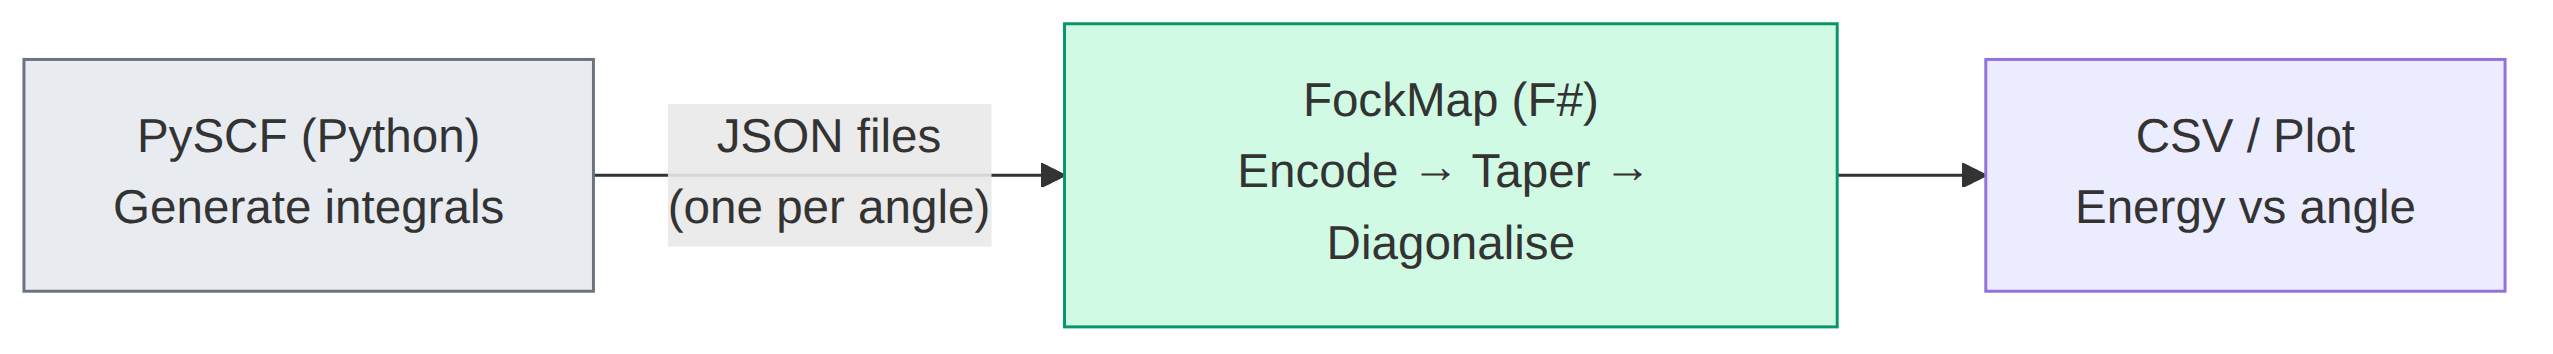
\includegraphics[keepaspectratio]{diagram-23.png}}

PySCF produces the molecular integrals (one JSON file per geometry);
FockMap reads them, applies the encoding pipeline, and outputs energies.
The JSON format is the same
\texttt{Map\textless{}string,\ Complex\textgreater{}} (keys like
\texttt{"0,1"} for one-body and \texttt{"0,1,2,3"} for two-body) that
every companion script uses.

\begin{center}\rule{0.5\linewidth}{0.5pt}\end{center}

\section{The Scan}\label{the-scan-1}

With the skeleton precomputed and the integrals generated, the scan
itself is remarkably concise:

\begin{Shaded}
\begin{Highlighting}[]
\OtherTok{open}\NormalTok{ System}\KeywordTok{.}\NormalTok{Numerics}
\OtherTok{open}\NormalTok{ Encodings}

\NormalTok{//}\CommentTok{ Precompute the Pauli structure once}
\KeywordTok{let}\NormalTok{ skeleton = computeHamiltonianSkeleton ternaryTreeTerms }\DecValTok{14}\NormalTok{u}

\KeywordTok{let}\NormalTok{ angles = }\OperatorTok{[|} \FloatTok{60.0}\NormalTok{ .. }\FloatTok{5.0}\NormalTok{ .. }\FloatTok{180.0} \OperatorTok{|]}

\KeywordTok{for}\NormalTok{ angle }\KeywordTok{in}\NormalTok{ angles }\KeywordTok{do}
\NormalTok{    //}\CommentTok{ Load integrals for this geometry}
    \KeywordTok{let}\NormalTok{ factory = loadIntegrals }\OperatorTok{(}\NormalTok{sprintf }\StringTok{"h2o\_integrals\_\%03.0f.json"}\NormalTok{ angle}\OperatorTok{)}

\NormalTok{    //}\CommentTok{ Build the Hamiltonian (fast — just multiplying precomputed strings by numbers)}
    \KeywordTok{let}\NormalTok{ ham = applyCoefficients skeleton factory}

\NormalTok{    //}\CommentTok{ Taper}
    \KeywordTok{let}\NormalTok{ tapered = taper defaultTaperingOptions ham}

\NormalTok{    //}\CommentTok{ The ground{-}state energy is the smallest eigenvalue of the Hamiltonian matrix.}
\NormalTok{    //}\CommentTok{ For 14 qubits (or \textasciitilde{}11 after tapering), exact diagonalisation is still feasible.}
\NormalTok{    //}\CommentTok{ exactGroundStateEnergy builds the 2\^{}n × 2\^{}n matrix and returns min(eigenvalues).}
    \KeywordTok{let}\NormalTok{ energy = exactGroundStateEnergy tapered.Hamiltonian}

\NormalTok{    printfn }\StringTok{"\%.0f°  \%.6f Ha"}\NormalTok{ angle energy}
\end{Highlighting}
\end{Shaded}

The inner loop --- \texttt{applyCoefficients}, \texttt{taper},
diagonalise --- runs in milliseconds per geometry. The entire 25-point
scan takes a few seconds on a laptop.

\begin{center}\rule{0.5\linewidth}{0.5pt}\end{center}

\section{The Result: Coarse Scan}\label{the-result-coarse-scan}

The coarse scan produces FCI energies at each geometry:

\begin{longtable}[]{@{}cccc@{}}
\toprule\noalign{}
Angle (°) & \(E\) (Ha) & Angle (°) & \(E\) (Ha) \\
\midrule\noalign{}
\endhead
\bottomrule\noalign{}
\endlastfoot
60 & −74.9277 & 110 & −75.0089 \\
70 & −74.9697 & 120 & −74.9966 \\
80 & −74.9963 & 130 & −74.9785 \\
90 & −75.0104 & 150 & −74.9328 \\
100 & −75.0140 & 180 & −74.8882 \\
105 & −75.0125 & & \\
\end{longtable}

The minimum is near \textbf{100°}, with energy dropping steeply on both
sides. The coarse scan tells us \emph{where to look} --- but the minimum
could be anywhere between 95° and 105°. This is exactly how a
computational chemist works: coarse grid first, then refine.

\begin{center}\rule{0.5\linewidth}{0.5pt}\end{center}

\section{Zooming In: Fine Scan}\label{zooming-in-fine-scan}

We re-run the scan from 95° to 115° in 1° steps. The skeleton is already
computed --- only the integrals change at each angle --- so this second
pass costs almost nothing:

\begin{longtable}[]{@{}cccc@{}}
\toprule\noalign{}
Angle (°) & \(E\) (Ha) & Angle (°) & \(E\) (Ha) \\
\midrule\noalign{}
\endhead
\bottomrule\noalign{}
\endlastfoot
95 & −75.013394 & 106 & −75.011934 \\
96 & −75.013706 & 107 & −75.011301 \\
97 & −75.013924 & 108 & −75.010591 \\
98 & −75.014051 & 109 & −75.009805 \\
\textbf{99} & \textbf{−75.014087} & 110 & −75.008946 \\
100 & −75.014034 & 112 & −75.007011 \\
101 & −75.013893 & 114 & −75.004798 \\
103 & −75.013356 & 115 & −75.003590 \\
105 & −75.012488 & & \\
\end{longtable}

The minimum is at \textbf{99°} with energy \textbf{−75.0141 Ha}. The
curve is clearly parabolic --- the energy changes by only 0.00005 Ha
between 98° and 100°, then drops away more steeply on either side.

\begin{figure}
\centering
\pandocbounded{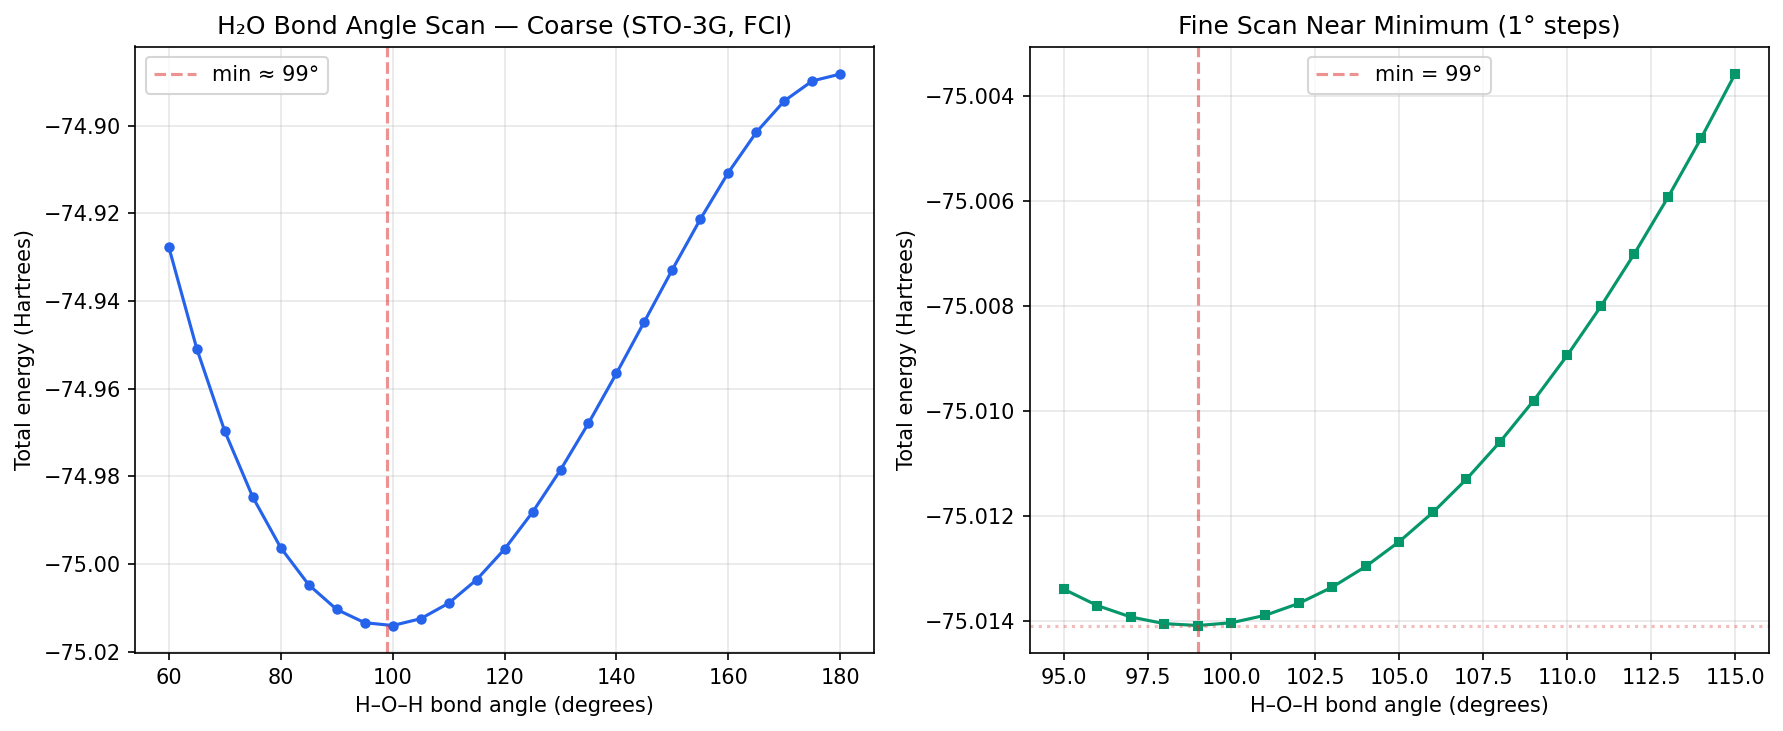
\includegraphics[keepaspectratio]{h2o_bond_angle.png}}
\caption{H₂O bond angle scan (STO-3G, FCI): coarse scan (left)
identifies the minimum near 100°; fine scan (right) pinpoints it at
99°.}
\end{figure}

\begin{center}\rule{0.5\linewidth}{0.5pt}\end{center}

\section{What Do the Numbers Mean?}\label{what-do-the-numbers-mean}

The minimum at \textbf{99°} in STO-3G is \textasciitilde5° below the
experimental value of 104.52°. The discrepancy comes from the minimal
basis set --- STO-3G uses only one Slater-type orbital per atomic
orbital, which is too inflexible to capture the fine details of electron
correlation near the equilibrium geometry. A larger basis set (cc-pVDZ,
cc-pVTZ) shifts the minimum toward the experimental value. At the
cc-pVTZ level, the computed angle is within 0.5° of experiment.

But the point is not the fourth decimal place. The point is the
\emph{method}: we derived a molecular geometry from a quantum simulation
pipeline. No one told the code that water should bend. No one
parameterised the angle. The pipeline explored the energy landscape and
found the bend --- the same bend that determines water's polarity, its
solvent properties, its ability to form hydrogen bonds, and ultimately,
its role in sustaining life on Earth.

\begin{center}\rule{0.5\linewidth}{0.5pt}\end{center}

\section{Why Does Water Bend?}\label{why-does-water-bend}

The energy curve tells us \emph{that} water bends. The density matrix
framework from Chapter 6 tells us \emph{why}.

At 180° (linear geometry), the molecular orbitals have a symmetry that
makes certain exchange integrals vanish. The off-diagonal terms in the
density matrix --- the ones that carry correlation energy --- are
constrained by symmetry. As the molecule bends, that symmetry breaks,
new exchange pathways open up, and the correlation energy drops. The
total energy decreases until the cost of nuclear repulsion (the two
hydrogen atoms getting closer) balances the gain in electron
correlation.

This is the deeper story: the bond angle is a compromise between nuclear
geometry and electronic correlation. VSEPR's ``lone pair repulsion'' is
a cartoon version of this --- qualitatively correct, but the real
mechanism is a balance of energies that only a full quantum treatment
can quantify.

\begin{center}\rule{0.5\linewidth}{0.5pt}\end{center}

\section{What About the Encoding?}\label{what-about-the-encoding}

With 14 spin-orbitals, H₂O is the first molecule in this book where
encoding choice makes a meaningful difference in circuit cost. If we
replace \texttt{ternaryTreeTerms} with \texttt{jordanWignerTerms} in the
skeleton, the energies don't change --- same physics --- but the Pauli
weights increase dramatically:

\begin{longtable}[]{@{}lcc@{}}
\toprule\noalign{}
Encoding & Max weight & Avg weight \\
\midrule\noalign{}
\endhead
\bottomrule\noalign{}
\endlastfoot
Jordan--Wigner & 14 & \textasciitilde7 \\
Bravyi--Kitaev & 5 & \textasciitilde3 \\
Parity & 14 & \textasciitilde7 \\
Binary Tree & 5 & \textasciitilde3 \\
Ternary Tree & 4 & \textasciitilde3 \\
\end{longtable}

The ternary tree encoding produces the lightest Pauli strings, which
translates directly to fewer CNOTs per Trotter step. This is the
compression we studied in Chapters 7 and 16 --- now applied to a
molecule large enough for it to matter.

For the energy \emph{scan}, the encoding doesn't affect the result (all
encodings give the same eigenvalues). But when we move to a quantum
computer --- where each CNOT carries noise --- the lighter encoding
gives a more accurate simulation for the same hardware budget. At H₂O
scale, that's roughly a 3× reduction in two-qubit gates.

\begin{center}\rule{0.5\linewidth}{0.5pt}\end{center}

\section{The Greenhouse Connection}\label{the-greenhouse-connection}

Water's bent shape isn't just a textbook fact --- it's one of the
reasons Earth supports life.

A bent molecule has a permanent electric dipole moment: the oxygen end
is slightly negative, the hydrogen end slightly positive. This dipole
oscillates during the bending vibration (\(\nu_2\) mode at \(\approx\)
1595 cm\(^{-1}\)), creating a time-varying electric field that couples
to infrared photons. That coupling is what makes water a greenhouse gas:
it absorbs outgoing infrared radiation and re-emits it in all
directions, warming the atmosphere.

A linear H₂O molecule would have no permanent dipole and a very
different infrared spectrum. The bond angle we just computed --- the one
that emerged from our pipeline without any empirical input --- is
literally the reason Earth has a habitable temperature.

The potential energy surface scan we performed is the first step in a
vibrational analysis. The \emph{curvature} of the energy curve near the
minimum (the second derivative) determines the bending frequency. This
is obtained from the \textbf{Hessian matrix} of the PES --- and
computing that Hessian for molecules where classical methods fail is one
of the practical applications of quantum simulation.

\begin{center}\rule{0.5\linewidth}{0.5pt}\end{center}

\section{Key Takeaways}\label{key-takeaways-18}

\begin{itemize}
\tightlist
\item
  A potential energy surface scan runs the \textbf{same pipeline} at
  many geometries and plots energy versus structural parameter.
\item
  The \textbf{skeleton API} separates structure (encoding-dependent,
  computed once) from coefficients (geometry-dependent, applied per
  point), making scans efficient.
\item
  The energy minimum of the H₂O bond angle scan occurs at \textbf{99°}
  in STO-3G --- close to the experimental 104.52°, with the discrepancy
  due to the minimal basis set.
\item
  The bond angle emerges from quantum mechanics without empirical input
  --- it's a balance of nuclear repulsion and electronic correlation.
\item
  Water's bent geometry produces its permanent dipole moment, which
  makes it a greenhouse gas and a universal solvent --- properties that
  follow directly from the energy curve we computed.
\end{itemize}

\begin{center}\rule{0.5\linewidth}{0.5pt}\end{center}

\chapter{Chapter 20: Algorithms --- VQE and
QPE}\label{chapter-20-algorithms-vqe-and-qpe}

\emph{Chapters 18 and 19 used exact diagonalisation as a stand-in energy
oracle. This chapter replaces that stand-in with the quantum algorithms
that run on real hardware.}

\section{In This Chapter}\label{in-this-chapter-19}

\begin{itemize}
\tightlist
\item
  \textbf{What you'll learn:} How the two major quantum chemistry
  algorithms --- VQE (variational, near-term) and QPE (phase estimation,
  fault-tolerant) --- consume the encoded Hamiltonian, and what
  measurement infrastructure they require.
\item
  \textbf{Why this matters:} FockMap produces the \emph{input} to these
  algorithms. Understanding what the algorithms need helps you make
  better encoding and tapering choices --- and understand why the CNOT
  counts from Chapter 17 matter so much.
\item
  \textbf{Prerequisites:} Chapters 17--19 (cost analysis, pipeline, bond
  angle scan).
\end{itemize}

\begin{center}\rule{0.5\linewidth}{0.5pt}\end{center}

\section{Two Algorithms, One Input}\label{two-algorithms-one-input}

In Chapters 18 and 19, we computed ground-state energies by exact
diagonalisation --- building the Hamiltonian as a matrix and finding its
smallest eigenvalue classically. For H₂ (\(2^4 = 16\)-dimensional
matrix) and H₂O in minimal basis (\(2^{11} = 2{,}048\)-dimensional after
tapering), exact diagonalisation is trivially feasible on a laptop. But
for larger systems --- N₂ (20 qubits → \(2^{20} \approx 10^6\)) or
FeMo-co (108 qubits → \(2^{108} \approx 10^{32}\)) --- the matrix does
not fit in any existing memory.

This is where quantum algorithms enter. Instead of building the
exponentially large matrix, a quantum computer prepares the state
directly in \(n\) qubits and extracts the energy through measurement.
The pipeline output --- the Pauli Hamiltonian
\(\hat{H} = \sum_k c_k P_k\) --- is exactly what these algorithms
consume.

There are two main approaches, and they make very different demands on
the hardware.

\textbf{VQE} (Variational Quantum Eigensolver) uses short circuits and
many measurements. It's designed for \emph{near-term} quantum computers
--- noisy devices with limited circuit depth but reasonable qubit
counts. The quantum computer prepares a trial state and measures Pauli
expectation values; a classical computer optimises the state parameters.

\textbf{QPE} (Quantum Phase Estimation) uses deep circuits and few
measurements. It's designed for \emph{fault-tolerant} quantum computers
--- devices with error correction, where circuit depth is not the
bottleneck. The quantum computer extracts the ground-state energy
directly via phase kickback.

Both algorithms consume the same object: a Pauli Hamiltonian
\(\hat{H} = \sum_k c_k P_k\) --- exactly what our pipeline produces.

\begin{center}\rule{0.5\linewidth}{0.5pt}\end{center}

\section{VQE: The Near-Term
Algorithm}\label{vqe-the-near-term-algorithm}

\subsection{The Loop}\label{the-loop}

VQE is fundamentally an optimisation loop. The quantum computer serves
as a function evaluator --- it takes parameters \(\boldsymbol{\theta}\)
and returns an energy estimate \(\langle\hat{H}\rangle_\theta\). The
classical computer adjusts \(\boldsymbol{\theta}\) to minimize the
energy.

\pandocbounded{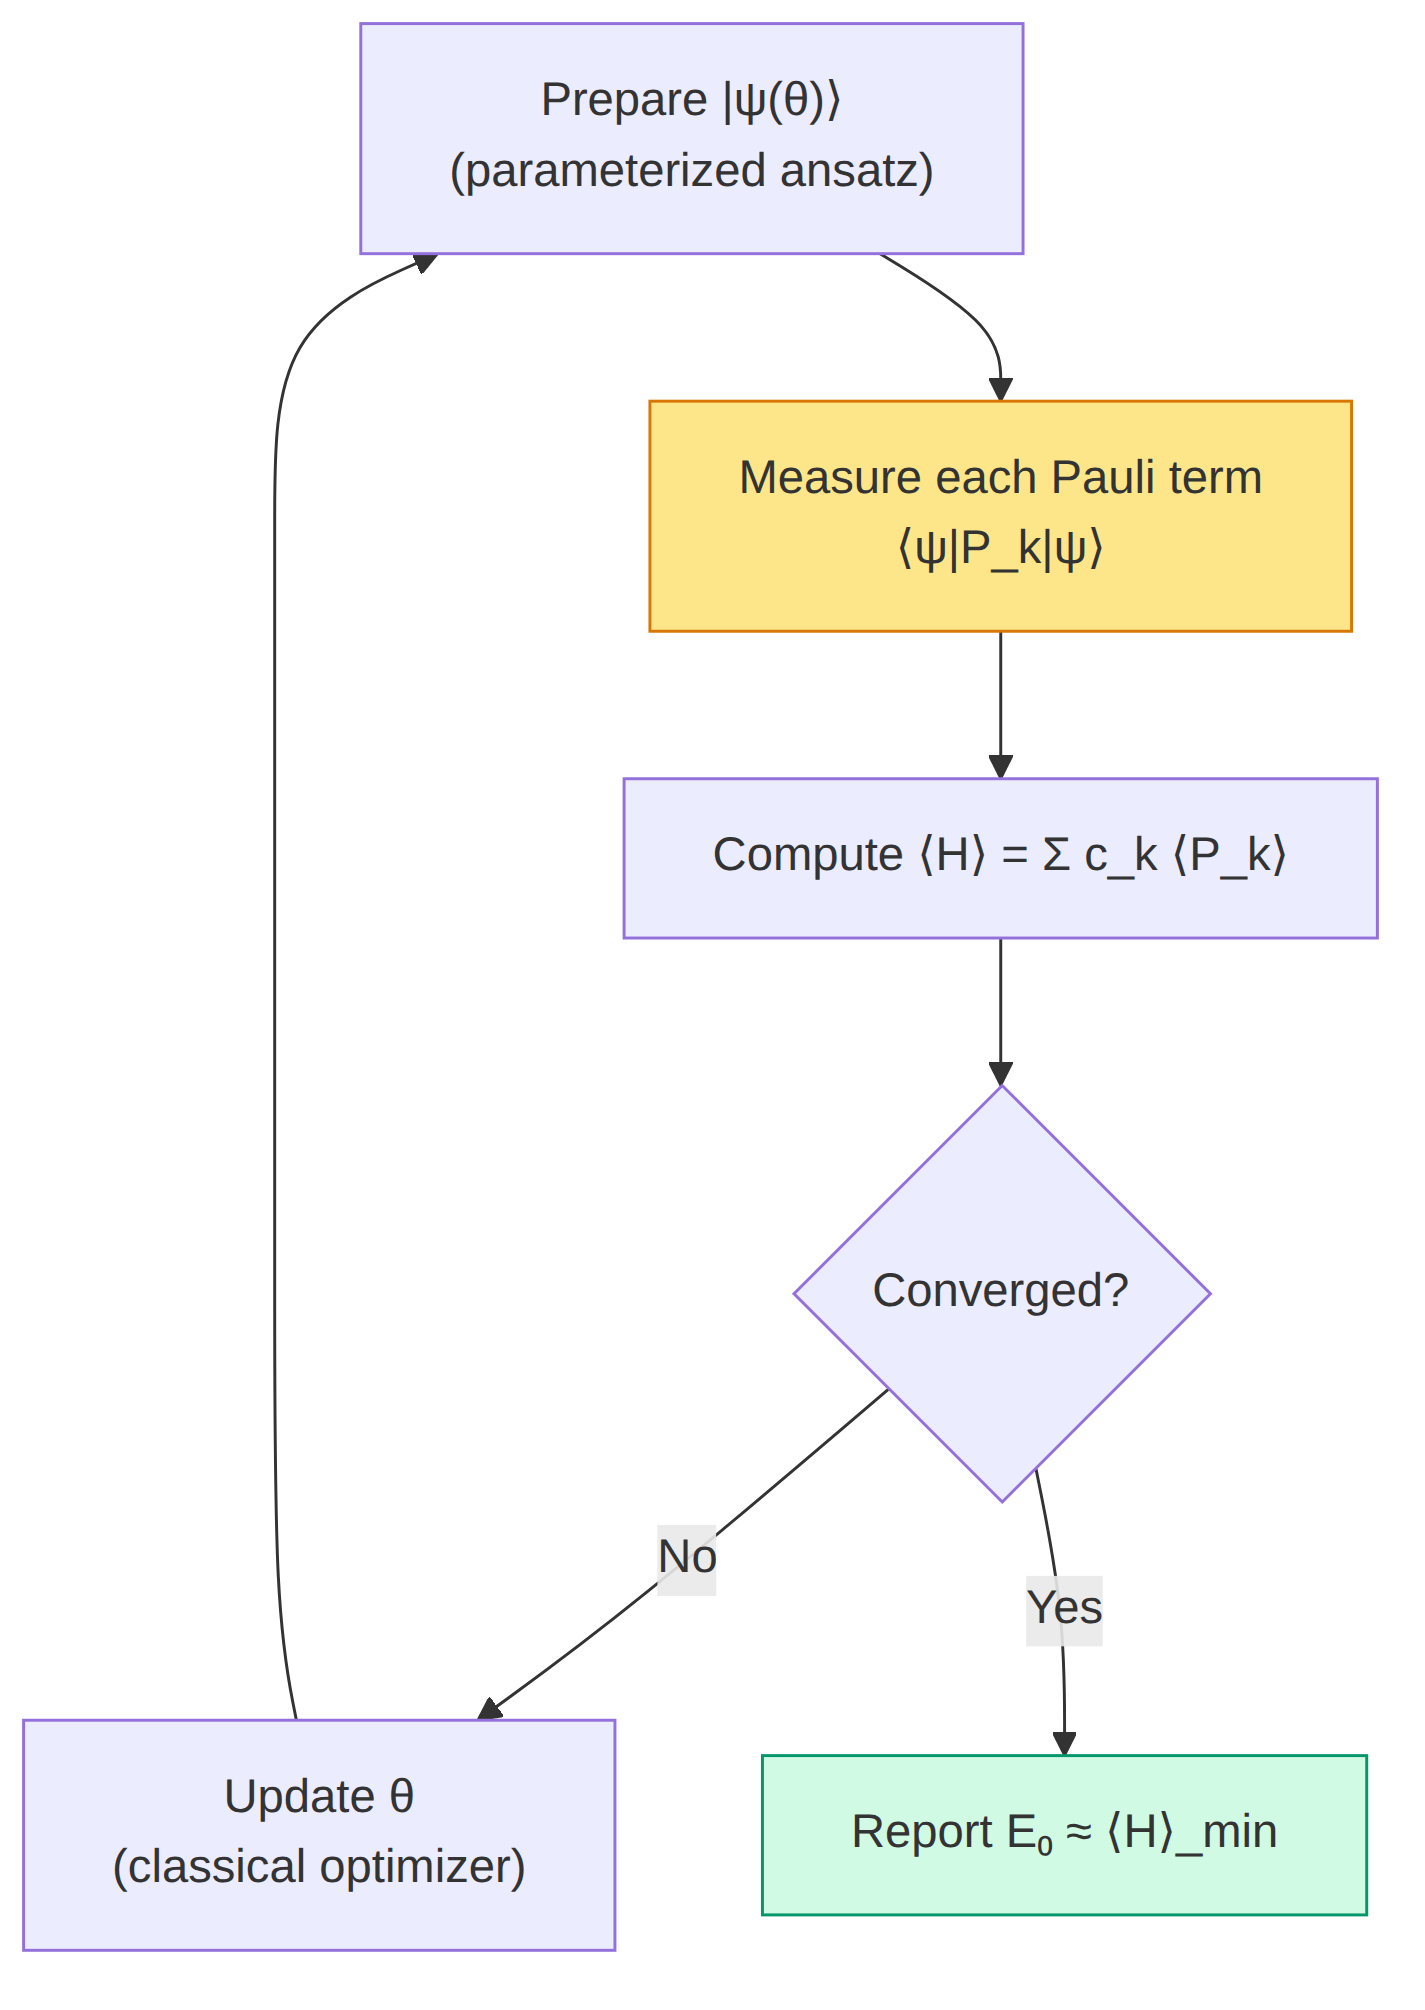
\includegraphics[keepaspectratio]{diagram-24.png}}

The yellow box is where FockMap's output matters most. Measuring
\(\langle P_k \rangle\) for each Pauli term in the Hamiltonian requires
a separate circuit --- or, better, measuring several commuting terms
simultaneously.

\subsection{Measurement Grouping}\label{measurement-grouping}

Not every Pauli term needs its own circuit. Two Pauli operators can be
measured simultaneously if they \textbf{qubit-wise commute} --- that is,
if they commute on every individual qubit position. For example, \(ZI\)
and \(ZZ\) qubit-wise commute (both have \(Z\) or \(I\) at each
position), so a single \(Z\)-basis measurement of all qubits yields both
expectation values.

FockMap groups the Hamiltonian terms automatically:

\begin{Shaded}
\begin{Highlighting}[]
\KeywordTok{let}\NormalTok{ program = groupCommutingTerms hamiltonian}
\NormalTok{printfn }\StringTok{"Total terms: \%d"}\NormalTok{ program.TotalTerms}
\NormalTok{printfn }\StringTok{"Measurement groups: \%d"}\NormalTok{ program.GroupCount}
\end{Highlighting}
\end{Shaded}

For the 15-term H₂ Hamiltonian, this typically produces 5 measurement
groups --- a 3× reduction in the number of distinct circuits needed.

The grouping matters because each distinct circuit must be run many
times (to accumulate statistics), and each additional group multiplies
the total measurement time. Fewer groups = faster VQE iterations.

\subsection{Shot Counts}\label{shot-counts}

Each measurement gives a binary outcome (\(\pm 1\)). To estimate the
expectation value \(\langle P_k \rangle\) to precision \(\delta\), you
need approximately \(1/\delta^2\) repetitions (``shots''). But where
does the total shot count formula come from? Let's derive it.

\textbf{The energy estimator.} The energy is
\(\langle\hat{H}\rangle = \sum_k c_k \langle P_k \rangle\). Each
\(\langle P_k \rangle\) is estimated from \(N_k\) measurement shots,
giving an estimator \(\hat{m}_k\) with variance
\(\text{Var}(\hat{m}_k) \leq 1/N_k\) (since each shot yields \(\pm 1\),
the variance of a single outcome is at most 1).

\textbf{Error propagation.} The variance of the total energy estimate
is:

\[\text{Var}(\hat{E}) = \sum_k c_k^2 \,\text{Var}(\hat{m}_k) \leq \sum_k \frac{c_k^2}{N_k}\]

\textbf{Optimal allocation.} If we have a total shot budget
\(N_\text{total} = \sum_k N_k\) and want to minimise
\(\text{Var}(\hat{E})\), Lagrange optimisation gives the optimal
allocation \(N_k \propto |c_k|\). Substituting back:

\[\text{Var}(\hat{E}) = \frac{1}{N_\text{total}} \left(\sum_k |c_k|\right)^2\]

\textbf{Setting the target.} For energy precision \(\epsilon\) (meaning
standard deviation \(\leq \epsilon\)), we need
\(\text{Var}(\hat{E}) \leq \epsilon^2\), giving:

\[N_\text{total} \geq \frac{1}{\epsilon^2}\left(\sum_k \lvert c_k\rvert\right)^2\]

This is the shot-count formula. The key quantity is the \textbf{1-norm}
\(\sum_k |c_k|\) --- it determines the measurement cost because terms
with larger coefficients contribute more variance and demand more shots.
This estimate assumes each Pauli term is measured independently (or in
qubit-wise commuting groups) and that the dominant error source is
finite sampling. In practice, correlated measurement strategies
(classical shadows, derandomisation) can improve the scaling, but the
1-norm estimate provides a useful and widely-cited baseline (Wecker et
al., Phys. Rev.~A 92, 042303, 2015).

Tapering reduces this norm (fewer terms, smaller coefficients), which is
yet another benefit that compounds with the qubit reduction.

\begin{Shaded}
\begin{Highlighting}[]
\KeywordTok{let}\NormalTok{ shots = estimateShots }\FloatTok{0.0016}\NormalTok{ hamiltonian  //}\CommentTok{ chemical accuracy = 1.6 mHa}
\NormalTok{printfn }\StringTok{"Estimated shots for chemical accuracy: \%d"}\NormalTok{ shots}
\end{Highlighting}
\end{Shaded}

For H₂: \(\sum|c_k| \approx 3.7\) Ha, giving \textasciitilde5 million
shots at chemical accuracy. For H₂O: the 1-norm is larger, and the shot
count grows accordingly. This is the practical bottleneck of VQE --- not
circuit depth, but measurement overhead.

\subsection{Where FockMap Fits}\label{where-fockmap-fits}

FockMap's contribution to VQE is everything \emph{before} the
measurement loop:

\begin{enumerate}
\def\labelenumi{\arabic{enumi}.}
\tightlist
\item
  \textbf{The Hamiltonian} \(\{c_k, P_k\}\) --- the list of Pauli terms
  and coefficients
\item
  \textbf{The measurement program} --- which terms to group and measure
  together
\item
  \textbf{The shot budget} --- how many measurements each group needs
\item
  \textbf{The Trotter circuit} --- used as the ansatz or as part of the
  state preparation
\end{enumerate}

The actual VQE loop --- parameter optimisation, circuit execution, shot
collection --- is handled by execution frameworks like Qiskit, Cirq, or
Quokka. FockMap produces the input they consume.

\begin{center}\rule{0.5\linewidth}{0.5pt}\end{center}

\section{QPE: The Fault-Tolerant
Algorithm}\label{qpe-the-fault-tolerant-algorithm}

\subsection{The Idea}\label{the-idea}

QPE doesn't optimise --- it \emph{reads out} the ground-state energy
directly, like a quantum spectrometer. The key insight: if we can
implement the time-evolution operator \(e^{-i\hat{H}t}\) as a quantum
circuit, then phase kickback extracts the eigenvalue.

This is where Trotterization becomes essential. The operator
\(e^{-i\hat{H}t}\) is approximated by a product of Pauli rotations ---
exactly the Trotter step from Chapter 15. QPE applies this operation
repeatedly, controlled by ancilla qubits, and reads the energy from the
ancilla register.

\subsection{The Circuit}\label{the-circuit}

The QPE circuit has two registers. The \textbf{ancilla register} (\(m\)
qubits, initialised to \(\lvert 0\rangle\), each put into superposition
with a Hadamard gate) controls repeated applications of the
time-evolution operator on the \textbf{system register} (which holds the
trial state \(\lvert\psi\rangle\)):

\begin{enumerate}
\def\labelenumi{\arabic{enumi}.}
\tightlist
\item
  Ancilla qubit \(j\) controls the application of \(U^{2^j}\) to the
  system register, where \(U = e^{-i\hat{H}t}\) is one Trotter step.
\item
  After all controlled operations, an inverse QFT on the ancilla
  register converts the accumulated phases into a binary representation
  of the energy eigenvalue.
\item
  Measuring the ancilla register yields \(m\) bits of the energy.
\end{enumerate}

The controlled-\(U^{2^j}\) operation applies \(2^j\) Trotter steps ---
so the highest ancilla qubit controls \(2^{m-1}\) steps. This is where
the circuit depth comes from --- and why QPE demands fault-tolerant
hardware.

The cost is dominated by the controlled Trotter steps. Each step
requires the same gates as a regular Trotter step (Chapter 16), plus
control logic --- roughly doubling the CNOT count per step.

\subsection{Resource Estimation}\label{resource-estimation}

For a target energy precision \(\epsilon\):

\begin{itemize}
\tightlist
\item
  \textbf{System qubits}: \(n\) (from the encoding, after tapering)
\item
  \textbf{Ancilla qubits}: \(m = \lceil\log_2(1/\epsilon)\rceil\) (one
  bit per digit of precision)
\item
  \textbf{Trotter steps per controlled-\(U\)}: enough to keep the
  Trotter error below \(\epsilon\)
\end{itemize}

\begin{Shaded}
\begin{Highlighting}[]
\KeywordTok{let}\NormalTok{ resources = qpeResources }\DecValTok{10}\NormalTok{ hamiltonian }\FloatTok{0.1}
\NormalTok{printfn }\StringTok{"System qubits:  \%d"}\NormalTok{ resources.SystemQubits}
\NormalTok{printfn }\StringTok{"Ancilla qubits: \%d"}\NormalTok{ resources.AncillaQubits}
\NormalTok{printfn }\StringTok{"Total CNOTs:    \%d"}\NormalTok{ resources.TotalCnots}
\NormalTok{printfn }\StringTok{"Circuit depth:  \%d"}\NormalTok{ resources.CircuitDepth}
\end{Highlighting}
\end{Shaded}

For H₂ at chemical accuracy (\textasciitilde10 bits of precision): -
System: 2--4 qubits (depending on tapering) - Ancilla: 10 qubits -
Total: \textasciitilde14 qubits, \textasciitilde10,000 CNOTs

For H₂O at chemical accuracy: - System: \textasciitilde11 qubits (after
tapering) - Ancilla: 10 qubits - Total: \textasciitilde21 qubits,
\textasciitilde500,000 CNOTs

The 50× jump from H₂ to H₂O is driven by two factors: more qubits (more
terms, heavier strings) and more Trotter steps (to keep the error small
for a larger Hamiltonian norm). This is why encoding choice and tapering
matter --- they reduce both factors.

\begin{center}\rule{0.5\linewidth}{0.5pt}\end{center}

\section{VQE vs QPE: A Summary}\label{vqe-vs-qpe-a-summary}

\begin{longtable}[]{@{}
  >{\raggedright\arraybackslash}p{(\linewidth - 4\tabcolsep) * \real{0.3333}}
  >{\raggedright\arraybackslash}p{(\linewidth - 4\tabcolsep) * \real{0.3333}}
  >{\raggedright\arraybackslash}p{(\linewidth - 4\tabcolsep) * \real{0.3333}}@{}}
\toprule\noalign{}
\begin{minipage}[b]{\linewidth}\raggedright
\end{minipage} & \begin{minipage}[b]{\linewidth}\raggedright
VQE
\end{minipage} & \begin{minipage}[b]{\linewidth}\raggedright
QPE
\end{minipage} \\
\midrule\noalign{}
\endhead
\bottomrule\noalign{}
\endlastfoot
\textbf{Hardware} & Near-term (noisy) & Fault-tolerant \\
\textbf{Circuit depth} & Short (one ansatz layer) & Deep (many Trotter
steps) \\
\textbf{Measurements} & Many (\(\sim 10^6\) shots) & Few (one
readout) \\
\textbf{Classical cost} & Optimisation loop & QFT + readout \\
\textbf{Bottleneck} & Shot count, barren plateaus & Circuit depth, error
correction \\
\textbf{FockMap provides} & Hamiltonian + measurement groups &
Hamiltonian + Trotter circuits \\
\end{longtable}

For the bond angle scan in Chapter 19, we used exact diagonalisation to
obtain the same target quantity that an ideal QPE calculation would
produce: the ground-state energy at each geometry. On real near-term
hardware, you would use VQE at each angle, accumulating enough shots to
estimate the energy to chemical accuracy. The structure of the scan is
the same; only the energy-evaluation subroutine changes.

\begin{center}\rule{0.5\linewidth}{0.5pt}\end{center}

\section{The Measurement Program in
Practice}\label{the-measurement-program-in-practice}

Let's look at the measurement infrastructure for H₂ in detail. The
15-term Hamiltonian groups into measurement bases:

\begin{Shaded}
\begin{Highlighting}[]
\KeywordTok{let}\NormalTok{ ham = computeHamiltonianWith jordanWignerTerms h2Factory }\DecValTok{4}\NormalTok{u}
\KeywordTok{let}\NormalTok{ program = groupCommutingTerms ham}

\KeywordTok{for}\NormalTok{ i }\KeywordTok{in} \DecValTok{0}\NormalTok{ .. program.Bases}\KeywordTok{.}\NormalTok{Length {-} }\DecValTok{1} \KeywordTok{do}
    \KeywordTok{let}\NormalTok{ basis = program.Bases}\KeywordTok{.}\OperatorTok{[}\NormalTok{i}\OperatorTok{]}
\NormalTok{    printfn }\StringTok{"Group \%d: \%d terms  (basis: \%s)"}
        \OperatorTok{(}\NormalTok{i + }\DecValTok{1}\OperatorTok{)}
\NormalTok{        basis.Terms}\KeywordTok{.}\NormalTok{Length}
        \OperatorTok{(}\NormalTok{basis.BasisRotation |\textgreater{} Array}\KeywordTok{.}\NormalTok{map }\DataTypeTok{string}\NormalTok{ |\textgreater{} String}\KeywordTok{.}\NormalTok{concat }\StringTok{""}\OperatorTok{)}
\end{Highlighting}
\end{Shaded}

A typical grouping might look like:

\begin{longtable}[]{@{}ccl@{}}
\toprule\noalign{}
Group & Terms & Measurement basis \\
\midrule\noalign{}
\endhead
\bottomrule\noalign{}
\endlastfoot
1 & 5 & ZZZZ (computational basis) \\
2 & 3 & XXXX \\
3 & 3 & XXYY \\
4 & 2 & YXXY \\
5 & 2 & YYXX \\
\end{longtable}

Group 1 contains all the diagonal (Z-only) terms --- they can all be
measured in the standard computational basis. The off-diagonal groups
each require basis rotations (Hadamard and S gates) before measurement.

This is the bridge between FockMap's algebraic output and the
experimental reality of a quantum computer: each group becomes a circuit
variant, each circuit runs thousands of times, and the statistics are
combined to estimate the energy.

\begin{center}\rule{0.5\linewidth}{0.5pt}\end{center}

\section{What FockMap Does --- and What It
Doesn't}\label{what-fockmap-does-and-what-it-doesnt}

FockMap's scope ends at circuit generation. It is important to be clear
about what lies \emph{outside} that scope:

\begin{itemize}
\tightlist
\item
  \textbf{Ansatz design}: VQE requires a parameterized circuit (ansatz).
  FockMap does not design ansätze --- it provides Trotter circuits and
  Pauli operator pools that downstream tools (Qiskit, tket, PennyLane)
  can use as building blocks.
\item
  \textbf{Classical optimisation}: the VQE optimisation loop (choosing
  \(\boldsymbol{\theta}\), handling barren plateaus, selecting an
  optimizer like L-BFGS or COBYLA) is handled by the execution
  framework, not FockMap.
\item
  \textbf{Hardware execution}: submitting circuits to real devices,
  managing job queues, handling device calibration --- all downstream.
\item
  \textbf{Error mitigation}: ZNE, PEC, symmetry verification --- these
  operate on measurement outcomes and are handled by execution
  frameworks. (FockMap's tapering symmetries are useful \emph{inputs} to
  symmetry verification, but FockMap doesn't implement the mitigation
  itself.)
\item
  \textbf{Noise modelling}: hardware noise interacts with both Trotter
  error and measurement error. FockMap's cost estimates are for
  \emph{ideal} (noiseless) circuits; real performance depends on device
  characteristics.
\end{itemize}

\begin{quote}
\textbf{Barren plateaus}, briefly: as the number of qubits grows,
randomly initialized VQE ansätze tend to produce cost function
landscapes where the gradient vanishes exponentially --- a phenomenon
called a barren plateau. This is a fundamental challenge for VQE at
scale, and it is one reason why adaptive methods (ADAPT-VQE) and
physically motivated ansätze (e.g., UCCSD) are preferred over
hardware-efficient random circuits.
\end{quote}

\begin{center}\rule{0.5\linewidth}{0.5pt}\end{center}

\section{Key Takeaways}\label{key-takeaways-19}

\begin{itemize}
\tightlist
\item
  \textbf{VQE} uses FockMap's Hamiltonian for measurement-based energy
  estimation. Fewer Pauli terms and lower 1-norm (from tapering)
  directly reduce the shot count.
\item
  \textbf{QPE} uses FockMap's Trotter circuits for phase estimation.
  Lower CNOT counts (from encoding choice) directly reduce the circuit
  depth.
\item
  \textbf{Measurement grouping} reduces the number of distinct circuits
  by combining qubit-wise commuting terms. FockMap does this
  automatically.
\item
  Both algorithms consume the same input --- the Pauli Hamiltonian ---
  but make different demands on the hardware. Encoding and tapering
  choices help both.
\end{itemize}

\begin{center}\rule{0.5\linewidth}{0.5pt}\end{center}

\chapter{Chapter 21: Speaking the Hardware's
Language}\label{chapter-21-speaking-the-hardwares-language}

\emph{The circuit exists in FockMap's type system. To run it on real
hardware, we need to speak the machine's language.}

\section{In This Chapter}\label{in-this-chapter-20}

\begin{itemize}
\tightlist
\item
  \textbf{What you'll learn:} How to export FockMap gate sequences as
  OpenQASM (universal), Q\# (Azure Quantum), or JSON (Python ecosystem)
  --- and when to use which.
\item
  \textbf{Why this matters:} A gate sequence that only exists in memory
  is a theoretical result. An exported circuit is an experiment you can
  run.
\item
  \textbf{Prerequisites:} Chapter 18 (the complete pipeline).
\end{itemize}

\begin{center}\rule{0.5\linewidth}{0.5pt}\end{center}

\section{Three Formats, One Circuit}\label{three-formats-one-circuit}

FockMap's Trotter decomposition (Chapter 16) produces a concrete gate
sequence --- an array of \texttt{Gate} values representing Hadamard, S,
CNOT, and Rz operations. That array is a platform-independent
description of the circuit. But to execute it, you need to express it in
a format that a quantum platform understands.

The three main targets:

\begin{longtable}[]{@{}
  >{\raggedright\arraybackslash}p{(\linewidth - 4\tabcolsep) * \real{0.3333}}
  >{\raggedright\arraybackslash}p{(\linewidth - 4\tabcolsep) * \real{0.3333}}
  >{\raggedright\arraybackslash}p{(\linewidth - 4\tabcolsep) * \real{0.3333}}@{}}
\toprule\noalign{}
\begin{minipage}[b]{\linewidth}\raggedright
Format
\end{minipage} & \begin{minipage}[b]{\linewidth}\raggedright
Ecosystem
\end{minipage} & \begin{minipage}[b]{\linewidth}\raggedright
Platforms
\end{minipage} \\
\midrule\noalign{}
\endhead
\bottomrule\noalign{}
\endlastfoot
\textbf{OpenQASM 3.0} & Universal standard & IBM Quantum, IonQ, Rigetti,
Amazon Braket \\
\textbf{Q\#} & Microsoft & Azure Quantum, QDK simulator \\
\textbf{JSON} & Python SDKs & Qiskit, Cirq, Quokka \\
\end{longtable}

FockMap can export to all three from the same gate array. The structure
is always the same: take the Trotter step, decompose it to gates,
export.

\begin{center}\rule{0.5\linewidth}{0.5pt}\end{center}

\section{OpenQASM: The Universal
Format}\label{openqasm-the-universal-format}

OpenQASM (Open Quantum Assembly Language) is maintained by IBM and
accepted by every major quantum platform. Version 3.0 supports qubit
declarations, standard gates, parameterized rotations, and classical
control.

\begin{Shaded}
\begin{Highlighting}[]
\KeywordTok{let}\NormalTok{ step = firstOrderTrotter }\FloatTok{0.1}\NormalTok{ hamiltonian}
\KeywordTok{let}\NormalTok{ gates = decomposeTrotterStep step}
\KeywordTok{let}\NormalTok{ qasm = toOpenQasm defaultOpenQasmOptions numQubits gates}
\NormalTok{printfn }\StringTok{"\%s"}\NormalTok{ qasm}
\end{Highlighting}
\end{Shaded}

The output looks like:

\begin{verbatim}
OPENQASM 3.0;
include "stdgates.inc";

qubit[2] q;

h q[0];
cx q[0], q[1];
rz(0.01234567) q[1];
cx q[0], q[1];
h q[0];
\end{verbatim}

Each Pauli rotation from Chapter 16 becomes a CNOT staircase bracketed
by basis-change gates. The angle in \texttt{rz()} is the rotation
parameter \(\theta = c_k \Delta t\).

\subsection{Gate Mapping}\label{gate-mapping}

\begin{longtable}[]{@{}ll@{}}
\toprule\noalign{}
FockMap Gate & OpenQASM \\
\midrule\noalign{}
\endhead
\bottomrule\noalign{}
\endlastfoot
\texttt{Gate.H\ i} & \texttt{h\ q{[}i{]};} \\
\texttt{Gate.S\ i} & \texttt{s\ q{[}i{]};} \\
\texttt{Gate.Sdg\ i} & \texttt{sdg\ q{[}i{]};} \\
\texttt{Gate.CNOT\ (c,\ t)} & \texttt{cx\ q{[}c{]},\ q{[}t{]};} \\
\texttt{Gate.Rz\ (i,\ θ)} & \texttt{rz(θ)\ q{[}i{]};} \\
\end{longtable}

\subsection{Configuration}\label{configuration}

\begin{Shaded}
\begin{Highlighting}[]
\KeywordTok{type}\NormalTok{ OpenQasmOptions =}
    \OperatorTok{\{}\NormalTok{ IncludeHeader : }\DataTypeTok{bool}\NormalTok{      //}\CommentTok{ "OPENQASM 3.0;" + include}
\NormalTok{      QubitName     : }\DataTypeTok{string}\NormalTok{    //}\CommentTok{ default: "q"}
\NormalTok{      Precision     : }\DataTypeTok{int}\NormalTok{       //}\CommentTok{ decimal places for angles}
\NormalTok{      Version       : QasmVersion }\OperatorTok{\}}\NormalTok{  //}\CommentTok{ V2 or V3}

\NormalTok{//}\CommentTok{ QASM 2.0 for Quokka compatibility}
\KeywordTok{let}\NormalTok{ qasm2 = toOpenQasm defaultOpenQasm2Options numQubits gates}
\end{Highlighting}
\end{Shaded}

QASM 2.0 differs in syntax (e.g., \texttt{qreg\ q{[}2{]};} instead of
\texttt{qubit{[}2{]}\ q;}) but the gate names are identical. Use V2 when
the target platform doesn't yet support V3.

\begin{center}\rule{0.5\linewidth}{0.5pt}\end{center}

\section{Q\#: Azure Quantum}\label{q-azure-quantum}

Q\# is Microsoft's quantum programming language, designed from the
ground up for expressing quantum algorithms.\footnote{The author was
  part of the team at Microsoft that created Q\#.} FockMap generates a
complete Q\# operation --- namespace, open statements, qubit allocation,
gate calls --- that you can compile and run on Azure Quantum or the
local QDK simulator.

\begin{Shaded}
\begin{Highlighting}[]
\KeywordTok{let}\NormalTok{ qsharp = toQSharp defaultQSharpOptions numQubits gates}
\NormalTok{printfn }\StringTok{"\%s"}\NormalTok{ qsharp}
\end{Highlighting}
\end{Shaded}

The output:

\begin{Shaded}
\begin{Highlighting}[]
\NormalTok{namespace FockMap.Generated \{}
\NormalTok{    open Microsoft.Quantum.Canon;}
\NormalTok{    open Microsoft.Quantum.Intrinsic;}

\NormalTok{    operation TrotterStep() : Unit \{}
\NormalTok{        use q = Qubit[2];}
\NormalTok{        H(q[0]);}
\NormalTok{        CNOT(q[0], q[1]);}
\NormalTok{        Rz(0.01234567, q[1]);}
\NormalTok{        CNOT(q[0], q[1]);}
\NormalTok{        H(q[0]);}
\NormalTok{    \}}
\NormalTok{\}}
\end{Highlighting}
\end{Shaded}

\subsection{Configuration}\label{configuration-1}

\begin{Shaded}
\begin{Highlighting}[]
\KeywordTok{type}\NormalTok{ QSharpOptions =}
    \OperatorTok{\{}\NormalTok{ Namespace     : }\DataTypeTok{string}\NormalTok{    //}\CommentTok{ default: "FockMap.Generated"}
\NormalTok{      OperationName : }\DataTypeTok{string}\NormalTok{    //}\CommentTok{ default: "TrotterStep"}
\NormalTok{      Precision     : }\DataTypeTok{int} \OperatorTok{\}}\NormalTok{     //}\CommentTok{ decimal places for angles}
\end{Highlighting}
\end{Shaded}

The generated operation is a pure gate sequence --- no measurement, no
classical control. The calling code (your VQE or QPE driver) allocates
the qubits, calls \texttt{TrotterStep()}, and handles measurement.

\begin{center}\rule{0.5\linewidth}{0.5pt}\end{center}

\section{JSON: The Python Bridge}\label{json-the-python-bridge}

Most quantum computing platforms have Python SDKs (Qiskit, Cirq,
PennyLane, Quokka). FockMap exports circuits as JSON that can be loaded
by any Python library:

\begin{Shaded}
\begin{Highlighting}[]
\KeywordTok{let}\NormalTok{ metadata = Map }\OperatorTok{[}
    \OperatorTok{(}\StringTok{"molecule"}\NormalTok{, }\StringTok{"H2"}\OperatorTok{)}
    \OperatorTok{(}\StringTok{"encoding"}\NormalTok{, }\StringTok{"ternary{-}tree"}\OperatorTok{)}
    \OperatorTok{(}\StringTok{"trotter\_order"}\NormalTok{, }\StringTok{"1"}\OperatorTok{)}
    \OperatorTok{(}\StringTok{"time\_step"}\NormalTok{, }\StringTok{"0.1"}\OperatorTok{)}
\OperatorTok{]}
\KeywordTok{let}\NormalTok{ json = toCircuitJson numQubits metadata gates}
\NormalTok{System}\KeywordTok{.}\NormalTok{IO}\KeywordTok{.}\NormalTok{File}\KeywordTok{.}\NormalTok{WriteAllText}\OperatorTok{(}\StringTok{"h2\_circuit.json"}\NormalTok{, json}\OperatorTok{)}
\end{Highlighting}
\end{Shaded}

The JSON schema:

\begin{Shaded}
\begin{Highlighting}[]
\FunctionTok{\{}
  \DataTypeTok{"num\_qubits"}\FunctionTok{:} \DecValTok{2}\FunctionTok{,}
  \DataTypeTok{"metadata"}\FunctionTok{:} \FunctionTok{\{}
    \DataTypeTok{"molecule"}\FunctionTok{:} \StringTok{"H2"}\FunctionTok{,}
    \DataTypeTok{"encoding"}\FunctionTok{:} \StringTok{"ternary{-}tree"}\FunctionTok{,}
    \DataTypeTok{"trotter\_order"}\FunctionTok{:} \StringTok{"1"}\FunctionTok{,}
    \DataTypeTok{"time\_step"}\FunctionTok{:} \StringTok{"0.1"}
  \FunctionTok{\},}
  \DataTypeTok{"gates"}\FunctionTok{:} \OtherTok{[}
    \FunctionTok{\{} \DataTypeTok{"type"}\FunctionTok{:} \StringTok{"H"}\FunctionTok{,} \DataTypeTok{"qubit"}\FunctionTok{:} \DecValTok{0} \FunctionTok{\}}\OtherTok{,}
    \FunctionTok{\{} \DataTypeTok{"type"}\FunctionTok{:} \StringTok{"CNOT"}\FunctionTok{,} \DataTypeTok{"control"}\FunctionTok{:} \DecValTok{0}\FunctionTok{,} \DataTypeTok{"target"}\FunctionTok{:} \DecValTok{1} \FunctionTok{\}}\OtherTok{,}
    \FunctionTok{\{} \DataTypeTok{"type"}\FunctionTok{:} \StringTok{"Rz"}\FunctionTok{,} \DataTypeTok{"qubit"}\FunctionTok{:} \DecValTok{1}\FunctionTok{,} \DataTypeTok{"angle"}\FunctionTok{:} \FloatTok{0.01234567} \FunctionTok{\}}\OtherTok{,}
    \FunctionTok{\{} \DataTypeTok{"type"}\FunctionTok{:} \StringTok{"CNOT"}\FunctionTok{,} \DataTypeTok{"control"}\FunctionTok{:} \DecValTok{0}\FunctionTok{,} \DataTypeTok{"target"}\FunctionTok{:} \DecValTok{1} \FunctionTok{\}}\OtherTok{,}
    \FunctionTok{\{} \DataTypeTok{"type"}\FunctionTok{:} \StringTok{"H"}\FunctionTok{,} \DataTypeTok{"qubit"}\FunctionTok{:} \DecValTok{0} \FunctionTok{\}}
  \OtherTok{]}
\FunctionTok{\}}
\end{Highlighting}
\end{Shaded}

On the Python side:

\begin{Shaded}
\begin{Highlighting}[]
\ImportTok{import}\NormalTok{ json}
\ImportTok{from}\NormalTok{ qiskit }\ImportTok{import}\NormalTok{ QuantumCircuit}

\ControlFlowTok{with} \BuiltInTok{open}\NormalTok{(}\StringTok{"h2\_circuit.json"}\NormalTok{) }\ImportTok{as}\NormalTok{ f:}
\NormalTok{    data }\OperatorTok{=}\NormalTok{ json.load(f)}

\NormalTok{qc }\OperatorTok{=}\NormalTok{ QuantumCircuit(data[}\StringTok{"num\_qubits"}\NormalTok{])}
\ControlFlowTok{for}\NormalTok{ g }\KeywordTok{in}\NormalTok{ data[}\StringTok{"gates"}\NormalTok{]:}
    \ControlFlowTok{if}\NormalTok{ g[}\StringTok{"type"}\NormalTok{] }\OperatorTok{==} \StringTok{"H"}\NormalTok{:}
\NormalTok{        qc.h(g[}\StringTok{"qubit"}\NormalTok{])}
    \ControlFlowTok{elif}\NormalTok{ g[}\StringTok{"type"}\NormalTok{] }\OperatorTok{==} \StringTok{"CNOT"}\NormalTok{:}
\NormalTok{        qc.cx(g[}\StringTok{"control"}\NormalTok{], g[}\StringTok{"target"}\NormalTok{])}
    \ControlFlowTok{elif}\NormalTok{ g[}\StringTok{"type"}\NormalTok{] }\OperatorTok{==} \StringTok{"Rz"}\NormalTok{:}
\NormalTok{        qc.rz(g[}\StringTok{"angle"}\NormalTok{], g[}\StringTok{"qubit"}\NormalTok{])}
    \ControlFlowTok{elif}\NormalTok{ g[}\StringTok{"type"}\NormalTok{] }\OperatorTok{==} \StringTok{"S"}\NormalTok{:}
\NormalTok{        qc.s(g[}\StringTok{"qubit"}\NormalTok{])}
    \ControlFlowTok{elif}\NormalTok{ g[}\StringTok{"type"}\NormalTok{] }\OperatorTok{==} \StringTok{"Sdg"}\NormalTok{:}
\NormalTok{        qc.sdg(g[}\StringTok{"qubit"}\NormalTok{])}
\end{Highlighting}
\end{Shaded}

The JSON format is deliberately simple --- flat list of gates, no nested
structures --- so that any Python library can consume it with a few
lines of code.

\begin{center}\rule{0.5\linewidth}{0.5pt}\end{center}

\section{Same Circuit, Three Formats}\label{same-circuit-three-formats}

Here is the full pipeline for H₂, exporting to all three formats:

\begin{Shaded}
\begin{Highlighting}[]
\KeywordTok{let}\NormalTok{ ham = computeHamiltonianWith ternaryTreeTerms factory }\DecValTok{4}\NormalTok{u}
\KeywordTok{let}\NormalTok{ tapered = taper defaultTaperingOptions ham}
\KeywordTok{let}\NormalTok{ step = firstOrderTrotter }\FloatTok{0.1}\NormalTok{ tapered.Hamiltonian}
\KeywordTok{let}\NormalTok{ gates = decomposeTrotterStep step}
\KeywordTok{let}\NormalTok{ n = tapered.TaperedQubitCount}

\NormalTok{//}\CommentTok{ OpenQASM 3.0}
\KeywordTok{let}\NormalTok{ qasm = toOpenQasm defaultOpenQasmOptions n gates}
\NormalTok{System}\KeywordTok{.}\NormalTok{IO}\KeywordTok{.}\NormalTok{File}\KeywordTok{.}\NormalTok{WriteAllText}\OperatorTok{(}\StringTok{"h2.qasm"}\NormalTok{, qasm}\OperatorTok{)}

\NormalTok{//}\CommentTok{ Q\#}
\KeywordTok{let}\NormalTok{ qs = toQSharp defaultQSharpOptions n gates}
\NormalTok{System}\KeywordTok{.}\NormalTok{IO}\KeywordTok{.}\NormalTok{File}\KeywordTok{.}\NormalTok{WriteAllText}\OperatorTok{(}\StringTok{"h2.qs"}\NormalTok{, qs}\OperatorTok{)}

\NormalTok{//}\CommentTok{ JSON (for Python/Qiskit)}
\KeywordTok{let}\NormalTok{ json = toCircuitJson n Map}\KeywordTok{.}\NormalTok{empty gates}
\NormalTok{System}\KeywordTok{.}\NormalTok{IO}\KeywordTok{.}\NormalTok{File}\KeywordTok{.}\NormalTok{WriteAllText}\OperatorTok{(}\StringTok{"h2.json"}\NormalTok{, json}\OperatorTok{)}

\NormalTok{printfn }\StringTok{"Exported \%d gates to 3 formats"}\NormalTok{ gates.Length}
\end{Highlighting}
\end{Shaded}

The gate array is the same in all three cases. Only the serialisation
differs.

\begin{center}\rule{0.5\linewidth}{0.5pt}\end{center}

\section{When to Use Which}\label{when-to-use-which}

\textbf{OpenQASM} is the safe default. Every major platform accepts it,
and QASM files are human-readable. Use QASM when: - You want maximum
portability - You're submitting to IBM Quantum, IonQ, or Amazon Braket -
You need a format that works with transpilation tools (Qiskit, tket)

\textbf{Q\#} when your target is Azure Quantum. The generated operation
integrates directly into the Q\# project system, with type checking and
resource estimation built in.

\textbf{JSON} when your workflow lives in Python. The JSON bridge lets
you construct the Hamiltonian and gate sequence in F\# (where the
algebra is exact) and run the circuit in Python (where the hardware SDKs
live). This is the ``best of both worlds'' approach: algebraic precision
in the construction, ecosystem breadth in the execution.

\begin{center}\rule{0.5\linewidth}{0.5pt}\end{center}

\section{What Export Does Not Solve}\label{what-export-does-not-solve}

FockMap's circuit export produces \emph{logical} circuits --- abstract
sequences of ideal gates. Before a logical circuit can run on real
hardware, several additional steps are required. These are handled by
platform-specific compilers (Qiskit transpiler, tket, Q\# resource
estimator), not by FockMap:

\begin{itemize}
\tightlist
\item
  \textbf{Native gate lowering}: hardware devices implement a small
  native gate set (e.g., \(\{\sqrt{X}, R_z, \text{CZ}\}\) for IBM,
  \(\{R_{xx}, GPI, GPI2\}\) for IonQ). The logical gates must be
  decomposed into the native set.
\item
  \textbf{Qubit routing}: physical qubits have limited connectivity
  (e.g., heavy-hex topology on IBM devices). SWAP gates must be inserted
  to bring non-adjacent qubits together for two-qubit gates. This can
  increase CNOT count by 2--5×.
\item
  \textbf{Circuit optimisation}: transpilers cancel redundant gates,
  commute operations to reduce depth, and apply template-matching
  identities. This typically reduces gate count by 20--40\% beyond
  FockMap's unoptimised output.
\item
  \textbf{Verification after import}: hardware compilers may reorder or
  decompose gates. Always verify that the transpiled circuit still
  produces the correct expectation values on a simulator before
  submitting to hardware.
\end{itemize}

\begin{center}\rule{0.5\linewidth}{0.5pt}\end{center}

\section{Verification Checklist}\label{verification-checklist}

Whichever format you choose, verify the output end-to-end:

\begin{enumerate}
\def\labelenumi{\arabic{enumi}.}
\tightlist
\item
  \textbf{Import} the circuit into the target platform (Qiskit, Q\#,
  Cirq)
\item
  \textbf{Simulate} with a statevector backend (zero noise, exact
  amplitudes)
\item
  \textbf{Compute} \(\langle\hat{H}\rangle\) from the statevector and
  compare against the exact eigenvalue from Chapter 9
\item
  \textbf{Transpile} to the target hardware's native gate set
\item
  \textbf{Re-simulate} the transpiled circuit and check that the energy
  is unchanged (within Trotter error)
\item
  \textbf{Only then} submit to real hardware or a noisy simulator
\end{enumerate}

For H₂, the exact FCI energy is \(-1.1373\) Ha (electronic only) or
\(-1.8572\) Ha (including nuclear repulsion). The Trotterised circuit
should produce an energy within \(O(\Delta t^2)\) of this --- typically
within 0.01 Ha at \(\Delta t = 0.1\). If the deviation is larger, check
the integral convention (Chapter 2) and the encoding consistency
(Chapter 9).

\begin{center}\rule{0.5\linewidth}{0.5pt}\end{center}

\section{Key Takeaways}\label{key-takeaways-20}

\begin{itemize}
\tightlist
\item
  FockMap exports to \textbf{three formats} from the same gate array:
  OpenQASM (universal), Q\# (Azure), JSON (Python).
\item
  The gate sequence is platform-independent; only the serialisation
  differs.
\item
  \textbf{OpenQASM} for portability, \textbf{Q\#} for Azure integration,
  \textbf{JSON} for Python workflows.
\item
  Always verify by comparing simulated expectation values against known
  eigenvalues.
\end{itemize}

\section{Further Reading}\label{further-reading-12}

\begin{itemize}
\tightlist
\item
  Svore, K. M. et al.~``Q\#: Enabling Scalable Quantum Computing and
  Development with a High-level DSL.'' arXiv:1803.00652 (2018). The
  design paper for Q\#.
\item
  Cross, A. W. et al.~``OpenQASM 3: A Broader and Deeper Quantum
  Assembly Language.'' ACM Transactions on Quantum Computing 3(3), 1--50
  (2022). The QASM 3.0 specification.
\end{itemize}

\begin{center}\rule{0.5\linewidth}{0.5pt}\end{center}

\chapter{Chapter 22: Scaling --- From H₂ to
FeMo-co}\label{chapter-22-scaling-from-hux2082-to-femo-co}

\emph{H₂ was our teacher. H₂O was our first real test. Now we look at
where the pipeline goes --- and where it meets its limits.}

\section{In This Chapter}\label{in-this-chapter-21}

\begin{itemize}
\tightlist
\item
  \textbf{What you'll learn:} How the pipeline's cost scales from small
  test systems through medium molecules to the grand challenge of
  quantum chemistry, and where encoding choice makes --- or breaks ---
  the simulation.
\item
  \textbf{Why this matters:} The promise of quantum simulation is that
  it handles molecules classical computers cannot. This chapter asks: at
  what point does that promise become real, and what does the hardware
  need to deliver?
\item
  \textbf{Prerequisites:} Chapters 17--19 (cost analysis, pipeline, bond
  angle scan).
\end{itemize}

\begin{center}\rule{0.5\linewidth}{0.5pt}\end{center}

\section{The Scaling Landscape}\label{the-scaling-landscape}

Every quantity in our pipeline grows with the number of spin-orbitals
\(n\):

\begin{longtable}[]{@{}
  >{\raggedright\arraybackslash}p{(\linewidth - 10\tabcolsep) * \real{0.1429}}
  >{\raggedright\arraybackslash}p{(\linewidth - 10\tabcolsep) * \real{0.1429}}
  >{\centering\arraybackslash}p{(\linewidth - 10\tabcolsep) * \real{0.1786}}
  >{\centering\arraybackslash}p{(\linewidth - 10\tabcolsep) * \real{0.1786}}
  >{\centering\arraybackslash}p{(\linewidth - 10\tabcolsep) * \real{0.1786}}
  >{\centering\arraybackslash}p{(\linewidth - 10\tabcolsep) * \real{0.1786}}@{}}
\toprule\noalign{}
\begin{minipage}[b]{\linewidth}\raggedright
Quantity
\end{minipage} & \begin{minipage}[b]{\linewidth}\raggedright
Growth
\end{minipage} & \begin{minipage}[b]{\linewidth}\centering
H₂ (\(n{=}4\))
\end{minipage} & \begin{minipage}[b]{\linewidth}\centering
H₂O (\(n{=}14\))
\end{minipage} & \begin{minipage}[b]{\linewidth}\centering
N₂ (\(n{=}20\))
\end{minipage} & \begin{minipage}[b]{\linewidth}\centering
FeMo-co (\(n{\approx}108\))
\end{minipage} \\
\midrule\noalign{}
\endhead
\bottomrule\noalign{}
\endlastfoot
Qubits & \(n\) & 4 & 14 & 20 & \textasciitilde108 \\
Hamiltonian terms & \(O(n^4)\) & 15 & \textasciitilde600 &
\textasciitilde2,000 & \textasciitilde{}\(10^7\) \\
JW max weight & \(n\) & 4 & 14 & 20 & 108 \\
TT max weight & \(O(\log_3 n)\) & 3 & 4 & 5 & \textasciitilde5 \\
Configurations (FCI) & \(\binom{n}{n_e}\) & 6 & 1,001 & 38,760 &
\textasciitilde{}\(10^{30}\) \\
\end{longtable}

The configuration count is why classical methods fail. Full CI (exact
diagonalisation) scales as \(\binom{n}{n_e}\) --- the number of ways to
place \(n_e\) electrons in \(n\) spin-orbitals. For FeMo-co, that's
roughly \(10^{30}\) determinants. No classical computer will ever
enumerate them.

A quantum computer doesn't enumerate configurations --- it represents
the quantum state directly in \(n\) qubits. The cost is in the
\emph{circuit}, not the \emph{state space}. And the circuit cost depends
on the encoding.

\begin{center}\rule{0.5\linewidth}{0.5pt}\end{center}

\section{The Encoding Crossover}\label{the-encoding-crossover}

At 4 qubits, all encodings cost the same (Chapter 18). At 14 qubits, the
differences appear (Chapter 19). Let's trace the crossover:

\begin{longtable}[]{@{}lcccc@{}}
\toprule\noalign{}
Molecule & \(n\) & JW CNOTs/step & TT CNOTs/step & Ratio \\
\midrule\noalign{}
\endhead
\bottomrule\noalign{}
\endlastfoot
H₂ & 4 & 12 & 12 & 1.0× \\
LiH & 12 & \textasciitilde400 & \textasciitilde200 & 2.0× \\
H₂O & 14 & \textasciitilde1,800 & \textasciitilde600 & 3.0× \\
N₂ & 20 & \textasciitilde8,000 & \textasciitilde2,000 & 4.0× \\
FeMo-co & \textasciitilde108 & \textasciitilde{}\(10^7\) &
\textasciitilde{}\(10^5\) & \textasciitilde100× \\
\end{longtable}

The ratio grows because JW's Pauli weights grow linearly while TT's grow
logarithmically. At FeMo-co scale, the difference is roughly two orders
of magnitude for the \emph{logical} (pre-transpilation) circuit. After
hardware-specific transpilation (qubit routing, native gate
decomposition), the absolute gate counts increase for all encodings, but
the \emph{relative} advantage of lighter Pauli weights is preserved.

\begin{quote}
\textbf{Caveat on the estimates:} The CNOT counts in this table are for
\emph{unoptimised logical circuits} --- the direct output of FockMap's
CNOT staircase decomposition. Hardware transpilers typically reduce
these by 20--40\% through gate cancellation, commutation, and template
matching. The estimates for N₂ and FeMo-co are order-of-magnitude
projections based on scaling trends, not computed values.
\end{quote}

\subsection{Why the Ratio Matters}\label{why-the-ratio-matters}

On near-term hardware, each CNOT gate has a finite error rate ---
typically 0.1--1\%. The probability that a circuit executes correctly
drops exponentially with the CNOT count:

\[P_\text{success} \approx (1 - \varepsilon)^{C_\text{CNOT}}\]

At \(\varepsilon = 0.5\%\) and 1,800 CNOTs (JW for H₂O),
\(P_\text{success} \approx 0.01\%\). At 600 CNOTs (TT for H₂O),
\(P_\text{success} \approx 5\%\). Under these typical assumptions,
that's roughly a 500× improvement in success probability from encoding
choice alone --- before error mitigation, before hardware improvements,
before anything else. (In practice, error mitigation techniques like
zero-noise extrapolation can partially compensate for low success rates,
but they impose their own sampling overhead.)

This is why the chapters on encoding (5--9), tapering (10--13), and cost
analysis (17) matter. They're not academic exercises. They directly
determine whether a simulation succeeds or fails on real hardware.

\begin{center}\rule{0.5\linewidth}{0.5pt}\end{center}

\section{The Tapering Dividend}\label{the-tapering-dividend}

Tapering compounds with encoding choice. At each system size, tapering
removes \(k\) qubits and often reduces the term count:

\begin{longtable}[]{@{}lcccc@{}}
\toprule\noalign{}
Molecule & \(n\) & Tapered \(n{-}k\) & Terms (before) & Terms (after) \\
\midrule\noalign{}
\endhead
\bottomrule\noalign{}
\endlastfoot
H₂ & 4 & 2 & 15 & 5 \\
H₂O & 14 & \textasciitilde11 & \textasciitilde600 &
\textasciitilde300 \\
N₂ & 20 & \textasciitilde16 & \textasciitilde2,000 &
\textasciitilde1,200 \\
\end{longtable}

Fewer terms means fewer Pauli rotations per Trotter step. Combined with
lower Pauli weights from a good encoding, the circuit shrinks
multiplicatively. The optimisation stack from Chapter 17 --- encoding +
tapering + Trotter order --- compounds at every scale.

\begin{center}\rule{0.5\linewidth}{0.5pt}\end{center}

\section{Application: Encoding Choice at H₂O
Scale}\label{application-encoding-choice-at-hux2082o-scale}

With 14 spin-orbitals, H₂O is the smallest molecule where encoding
choice makes a practical difference. Here's the full comparison after
tapering:

\begin{longtable}[]{@{}lcccc@{}}
\toprule\noalign{}
Encoding & Tapered qubits & Max weight & CNOTs/step & Depth estimate \\
\midrule\noalign{}
\endhead
\bottomrule\noalign{}
\endlastfoot
Jordan--Wigner & \textasciitilde11 & 11 & \textasciitilde1,800 &
\textasciitilde3,600 \\
Bravyi--Kitaev & \textasciitilde11 & 5 & \textasciitilde750 &
\textasciitilde1,500 \\
Parity & \textasciitilde11 & 11 & \textasciitilde1,800 &
\textasciitilde3,600 \\
Binary Tree & \textasciitilde11 & 5 & \textasciitilde700 &
\textasciitilde1,400 \\
Ternary Tree & \textasciitilde11 & 4 & \textasciitilde600 &
\textasciitilde1,200 \\
\end{longtable}

The 3× reduction from JW to TT is the difference between a circuit that
fries on near-term hardware and one that might just survive. On a device
with \textasciitilde99.5\% two-qubit gate fidelity, the TT circuit has
roughly a 10× higher success probability per shot. Over millions of VQE
shots, that translates directly to better energy estimates.

This is the practical answer to ``which encoding should I use?'' --- at
H₂O scale and beyond, ternary tree with tapering is the best option in
the FockMap toolkit.

\begin{center}\rule{0.5\linewidth}{0.5pt}\end{center}

\section{The Grand Challenge:
FeMo-co}\label{the-grand-challenge-femo-co}

The iron-molybdenum cofactor (FeMo-co) of nitrogenase is the molecule
that launched a field. It catalyses nitrogen fixation --- converting
atmospheric N₂ to ammonia --- and understanding its mechanism could
transform fertiliser production, one of the most energy-intensive
industrial processes on Earth.

FeMo-co has \textasciitilde54 active electrons in \textasciitilde108
active spin-orbitals. Classical methods cannot accurately compute its
electronic structure because the iron centres are \textbf{strongly
correlated}: many electron configurations contribute comparably to the
ground state, defeating perturbation theory and single-reference methods
like coupled cluster.

\subsection{The Numbers}\label{the-numbers-1}

\begin{longtable}[]{@{}ll@{}}
\toprule\noalign{}
Quantity & Value \\
\midrule\noalign{}
\endhead
\bottomrule\noalign{}
\endlastfoot
Active electrons & \textasciitilde54 \\
Active spin-orbitals & \textasciitilde108 \\
Qubits (JW) & \textasciitilde108 \\
JW max Pauli weight & 108 \\
TT max Pauli weight & \textasciitilde5 \\
JW CNOTs per worst-case rotation & 214 \\
TT CNOTs per worst-case rotation & 8 \\
Ratio & 27× \\
\end{longtable}

At 108 qubits, the JW encoding produces Pauli strings where nearly every
qubit participates. Each off-diagonal rotation requires a CNOT staircase
spanning the entire register. The ternary tree encoding compresses the
worst-case weight to \textasciitilde5 --- a chain of 4 CNOTs per
direction.

\subsection{How Far Away Is the
Hardware?}\label{how-far-away-is-the-hardware}

For FeMo-co at chemical accuracy via QPE: - \textbf{Qubits needed}:
\textasciitilde108 system + \textasciitilde10 ancilla ≈ 120 logical
qubits - \textbf{Trotter steps}: \textasciitilde{}\(10^4\) (for the
required precision) - \textbf{CNOTs per Trotter step} (TT):
\textasciitilde{}\(10^5\) - \textbf{Total CNOTs}:
\textasciitilde{}\(10^9\)

At current error rates, this requires full quantum error correction ---
perhaps 1,000--10,000 physical qubits per logical qubit, depending on
the code and hardware. That puts the total physical qubit count at
\(10^5\)--\(10^6\).

No device available today can do this. But the same pipeline we
developed for H₂ (4 qubits, 15 terms, 12 CNOTs) is the \emph{same code}
that would generate the FeMo-co circuit. The bottleneck is hardware, not
software. When the hardware arrives, the pipeline is ready.

\begin{center}\rule{0.5\linewidth}{0.5pt}\end{center}

\section{Where Classical Methods Still
Win}\label{where-classical-methods-still-win}

It's worth being honest about the landscape. Quantum simulation has a
theoretical advantage for strongly correlated systems, but classical
methods are formidable:

\begin{itemize}
\tightlist
\item
  \textbf{Density functional theory (DFT)} handles hundreds of atoms
  routinely. It's not exact, but it's remarkably accurate for weakly
  correlated systems and costs \(O(n^3)\).
\item
  \textbf{Coupled cluster CCSD(T)} --- the ``gold standard'' of quantum
  chemistry --- handles up to \textasciitilde50 atoms with chemical
  accuracy for single-reference systems.
\item
  \textbf{DMRG and tensor network methods} exploit the entanglement
  structure of 1D and quasi-1D systems, often matching quantum
  simulation accuracy for those geometries.
\end{itemize}

Quantum simulation's niche is the strongly correlated regime:
transition-metal complexes, open-shell systems, conical intersections,
and exotic electronic states where no classical method converges
reliably. FeMo-co is the poster child, but the real impact may be in
catalysis design, high-temperature superconductors, and photochemistry
--- areas where electron correlation defies classical approximation.

\begin{center}\rule{0.5\linewidth}{0.5pt}\end{center}

\section{Key Takeaways}\label{key-takeaways-21}

\begin{itemize}
\tightlist
\item
  Circuit cost grows with system size, but \textbf{encoding choice}
  determines the growth rate: linear (JW) vs logarithmic (TT) Pauli
  weight.
\item
  The \textbf{encoding crossover} becomes meaningful around 12--14
  qubits --- exactly the range of near-term quantum hardware.
\item
  \textbf{Tapering compounds} with encoding choice, reducing both qubit
  count and term count multiplicatively.
\item
  \textbf{FeMo-co} (\textasciitilde108 qubits) is the grand challenge:
  classically intractable, but requiring fault-tolerant hardware that
  doesn't yet exist.
\item
  The same pipeline code works at every scale --- from H₂ to FeMo-co.
  The bottleneck is hardware, not software.
\end{itemize}

\begin{center}\rule{0.5\linewidth}{0.5pt}\end{center}

\chapter{Chapter 23: What Comes Next}\label{chapter-23-what-comes-next}

\emph{The pipeline is complete. The book is almost over. But the field
is just getting started.}

\section{In This Chapter}\label{in-this-chapter-22}

\begin{itemize}
\tightlist
\item
  \textbf{What you'll learn:} What lies beyond this book --- the
  extensions, open problems, and emerging directions that build on the
  foundation we've laid.
\item
  \textbf{Why this matters:} A pipeline is only as useful as the
  questions it can answer. This chapter maps out where those questions
  lead.
\item
  \textbf{Prerequisites:} The whole book (but especially Chapters
  18--22).
\end{itemize}

\begin{center}\rule{0.5\linewidth}{0.5pt}\end{center}

\section{What We Built}\label{what-we-built}

Let's take a final inventory. Over twenty-three chapters, we constructed
a complete pipeline:

\pandocbounded{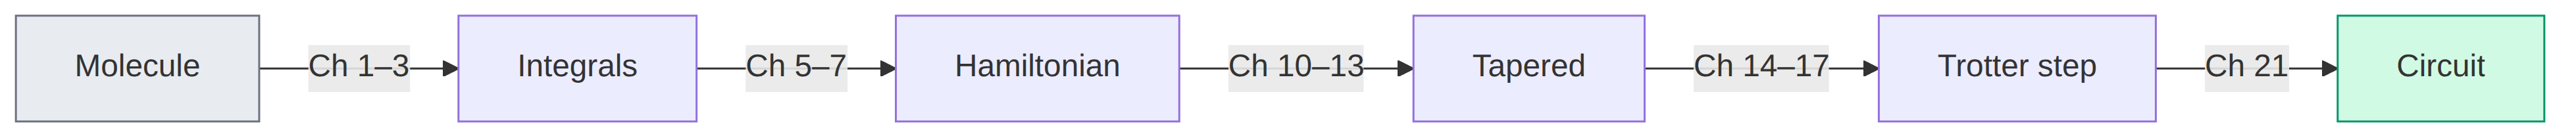
\includegraphics[keepaspectratio]{diagram-25.png}}

Every arrow is a function call in FockMap. Every box has been tested on
H₂ and applied to H₂O. The pipeline is real, open-source, and published
on NuGet.

But a pipeline is an instrument, not a destination. Here's where the
instrument gets used.

\begin{center}\rule{0.5\linewidth}{0.5pt}\end{center}

\section{Near-Term Extensions}\label{near-term-extensions}

\subsection{Circuit Optimisation}\label{circuit-optimisation}

FockMap currently produces \emph{unoptimised} gate sequences --- each
Pauli rotation becomes a CNOT staircase exactly as described in Chapter
16. Real quantum compilers (Qiskit's transpiler, Cambridge Quantum's
tket, BQSKit) apply additional transformations:

\begin{itemize}
\tightlist
\item
  \textbf{Gate cancellation}: adjacent CNOT pairs cancel.
  Identity-equivalent sequences are removed.
\item
  \textbf{Commutation-based reordering}: Pauli rotations that commute
  can be reordered to bring cancellable gates adjacent.
\item
  \textbf{Template matching}: known circuit identities replace expensive
  subcircuits with cheaper equivalents.
\item
  \textbf{Hardware-aware routing}: map logical qubits to physical
  qubits, inserting SWAP gates as needed for limited connectivity.
\end{itemize}

These optimisations typically reduce CNOT count by 20--40\% beyond what
FockMap produces. They operate on the gate-level output (QASM, Q\#, or
JSON) and don't require changes to the Hamiltonian construction.

\subsection{Error Mitigation}\label{error-mitigation}

Near-term quantum computers are noisy. Error mitigation techniques
extract better estimates from noisy circuits without the overhead of
full error correction:

\begin{itemize}
\tightlist
\item
  \textbf{Zero-noise extrapolation (ZNE)}: run the circuit at several
  artificial noise levels, then extrapolate to the zero-noise limit.
\item
  \textbf{Probabilistic error cancellation (PEC)}: represent the ideal
  circuit as a linear combination of noisy circuits and sample the
  combination.
\item
  \textbf{Symmetry verification}: post-select on measurement outcomes
  that satisfy known symmetries of the Hamiltonian (our tapering
  symmetries from Chapter 11 are ideal for this).
\end{itemize}

FockMap's contribution is the symmetry information: the Z₂ generators,
Clifford rotations, and parity sectors from the tapering analysis
provide exactly the symmetry constraints that verification-based
mitigation needs.

\subsection{Adaptive Ansätze}\label{adaptive-ansuxe4tze}

VQE (Chapter 20) uses a fixed ansatz --- a predetermined circuit
structure with adjustable parameters. Adaptive methods grow the ansatz
one operator at a time:

\begin{itemize}
\tightlist
\item
  \textbf{ADAPT-VQE}: at each iteration, select the Pauli operator from
  the Hamiltonian pool that gives the steepest energy gradient, add it
  to the ansatz, and re-optimise.
\item
  \textbf{Qubit-ADAPT}: same idea, but using single-qubit and two-qubit
  operators instead of full Pauli strings.
\end{itemize}

FockMap's Pauli-level representation of the Hamiltonian provides the
operator pool that ADAPT-VQE selects from. The encoding choice affects
the pool --- lighter Pauli strings make better ADAPT operators, which is
another argument for ternary tree encoding at scale.

\begin{center}\rule{0.5\linewidth}{0.5pt}\end{center}

\section{Bosonic Simulation}\label{bosonic-simulation}

FockMap already supports bosonic ladder operators and three
bosonic-to-qubit encodings (unary, binary, Gray code --- see the API
documentation). The natural extension is \textbf{vibronic simulation}:
mixed electron-phonon systems where both fermions and bosons are
present.

Applications include: - \textbf{Molecular vibrations}: the bond angle
scan in Chapter 19 gives the equilibrium geometry; the \emph{curvature}
of the PES gives vibrational frequencies. Concretely, a
finite-difference Hessian --- computed by running the same pipeline at
slightly displaced geometries --- yields the force-constant matrix.
Diagonalizing it (mass-weighted) produces the normal modes and harmonic
frequencies, which connect directly to infrared and Raman spectroscopy.
The entire calculation uses no machinery beyond what this book has
already built: repeat the pipeline at a few geometries, take numerical
derivatives, and diagonalize a small matrix. This is real computational
chemistry --- the same workflow that production codes use to predict
molecular spectra. - \textbf{Polaron physics}: electron-phonon coupling
in materials science, where an electron ``dressed'' by lattice
distortions has different effective mass and mobility. -
\textbf{Photochemistry}: conical intersections and non-adiabatic
dynamics, where nuclear and electronic motion couple strongly.

The encoding pipeline for bosonic modes parallels the fermionic one:
ladder operators → Pauli strings → Hamiltonian assembly. The main
difference is that bosonic modes require a truncation parameter \(d\)
(the maximum occupation number per mode), and the encoding choice
affects how many qubits each mode costs.

\begin{center}\rule{0.5\linewidth}{0.5pt}\end{center}

\section{Lattice Models}\label{lattice-models}

The second-quantised framework isn't limited to molecules. Lattice
models in condensed matter physics use the same operator algebra:

\begin{itemize}
\tightlist
\item
  \textbf{Hubbard model}: electrons hopping on a lattice with on-site
  repulsion. The same ladder operators, the same encodings, the same
  tapering --- different integrals.
\item
  \textbf{Heisenberg model}: spin-spin interactions on a lattice.
  Already expressed in Pauli operators --- no encoding step needed.
\item
  \textbf{Fermi-Hubbard at half-filling}: a testing ground for quantum
  advantage, where classical methods (DMRG, QMC) have known limitations
  in 2D.
\end{itemize}

FockMap's encoding and tapering infrastructure applies directly to these
systems. The Hamiltonian assembly step simplifies (lattice models have
regular structure), but the downstream pipeline --- Trotter
decomposition, cost analysis, circuit export --- is identical.

\begin{center}\rule{0.5\linewidth}{0.5pt}\end{center}

\section{Quantum Error Correction}\label{quantum-error-correction}

The tapering machinery from Chapters 10--13 is, at its core, stabiliser
theory: finding commuting Pauli operators that generate a symmetry
group, and using Clifford rotations to diagonalise them. This is
precisely the mathematical framework of quantum error-correcting codes.

\begin{itemize}
\tightlist
\item
  \textbf{Stabiliser codes} (surface code, Steane code, etc.) encode
  logical qubits into physical qubits using a stabiliser group --- a set
  of commuting Pauli operators whose simultaneous eigenspace defines the
  code space.
\item
  \textbf{Syndrome measurement} detects errors by measuring the
  stabilisers, exactly as our tapering step measures the Z₂ generators.
\item
  \textbf{Logical operators} act within the code space, just as our
  tapered Hamiltonian acts within the symmetry sector.
\end{itemize}

The algebra is the same. The difference is intent: tapering exploits
physical symmetries to reduce qubit count, while error correction
engineers artificial symmetries to detect and correct errors. A reader
who has understood Chapters 10--13 has already learned half of quantum
error correction theory.

\begin{center}\rule{0.5\linewidth}{0.5pt}\end{center}

\section{Open Problems}\label{open-problems}

Some questions this book doesn't answer --- because nobody has yet:

\begin{enumerate}
\def\labelenumi{\arabic{enumi}.}
\item
  \textbf{Optimal encoding}: is there a provably optimal encoding for a
  given Hamiltonian? The ternary tree encoding achieves \(O(\log_3 n)\)
  worst-case weight, which matches a known lower bound for balanced
  trees. But the best encoding might depend on the Hamiltonian's
  structure (sparsity, symmetry, locality), not just \(n\).
\item
  \textbf{Tapering beyond Z₂}: our tapering removes symmetries that
  square to the identity (Z₂ symmetries). What about higher-order
  symmetries --- U(1) particle number conservation, SU(2) spin symmetry?
  These could remove more qubits, but the Clifford rotation synthesis is
  harder.
\item
  \textbf{Trotter error bounds}: how many Trotter steps do you actually
  need? Tight error bounds for product formulas are an active area of
  research. Tighter bounds mean shorter circuits, which means earlier
  quantum advantage.
\item
  \textbf{Classical simulation limits}: where exactly does classical
  simulation become infeasible? DMRG and tensor network methods keep
  improving. The crossover point --- where quantum simulation beats the
  best classical method --- shifts with every algorithmic advance on
  both sides.
\end{enumerate}

\begin{center}\rule{0.5\linewidth}{0.5pt}\end{center}

\section{The Pipeline Is Ready}\label{the-pipeline-is-ready}

We'll end where we began. Chapter 1 asked: \emph{given a molecule, what
is its ground-state energy?} Twenty-two chapters later, we have a
complete, tested, open-source pipeline that answers the question --- for
any fermionic or bosonic system, with six encoding options,
symmetry-based tapering, first and second-order Trotterization, and
export to every major quantum platform.

The pipeline runs on a laptop for small molecules (H₂, LiH). It produces
circuits that near-term hardware can attempt for medium molecules (H₂O,
N₂). And it generates the circuits that fault-tolerant hardware will
need for the molecules that actually matter (FeMo-co, transition-metal
catalysts, photochemical systems).

The H₂ dissociation curve in Chapter 18 showed the pipeline's
correctness. The water bond angle scan in Chapter 19 showed its
predictive power --- we computed a molecular geometry from first
principles. The same machinery, with bigger integrals and more qubits,
will someday compute the geometry of a catalyst, the spectrum of a
photoactive molecule, or the mechanism of nitrogen fixation.

The quantum computer isn't ready yet. The pipeline is.

\begin{center}\rule{0.5\linewidth}{0.5pt}\end{center}

\section{Key Takeaways}\label{key-takeaways-22}

\begin{itemize}
\tightlist
\item
  \textbf{Circuit optimisation}, \textbf{error mitigation}, and
  \textbf{adaptive ansätze} build directly on FockMap's output.
\item
  \textbf{Bosonic simulation} extends the same pipeline to
  electron-phonon systems, vibrations, and photochemistry.
\item
  \textbf{Lattice models} use the same operator algebra and encoding
  infrastructure.
\item
  \textbf{Quantum error correction} uses the same stabiliser theory as
  tapering --- different intent, same mathematics.
\item
  The pipeline works at every scale. The bottleneck is hardware, not
  software.
\end{itemize}

\begin{center}\rule{0.5\linewidth}{0.5pt}\end{center}

\chapter{Appendix A: Library Cookbook
Reference}\label{appendix-a-library-cookbook-reference}

\emph{A quick-reference guide to every public type and function in
FockMap.}

This appendix summarizes the 15-chapter Cookbook that accompanies the
main text. For full worked examples, see the
\href{../docs/guides/cookbook/index.html}{Cookbook} on the companion
website.

\begin{center}\rule{0.5\linewidth}{0.5pt}\end{center}

\section{Type System at a Glance}\label{type-system-at-a-glance}

\begin{longtable}[]{@{}
  >{\raggedright\arraybackslash}p{(\linewidth - 4\tabcolsep) * \real{0.3077}}
  >{\raggedright\arraybackslash}p{(\linewidth - 4\tabcolsep) * \real{0.3077}}
  >{\centering\arraybackslash}p{(\linewidth - 4\tabcolsep) * \real{0.3846}}@{}}
\toprule\noalign{}
\begin{minipage}[b]{\linewidth}\raggedright
Type
\end{minipage} & \begin{minipage}[b]{\linewidth}\raggedright
What it represents
\end{minipage} & \begin{minipage}[b]{\linewidth}\centering
Chapter
\end{minipage} \\
\midrule\noalign{}
\endhead
\bottomrule\noalign{}
\endlastfoot
\texttt{Pauli} & Single-qubit operator: I, X, Y, Z & 1 \\
\texttt{Phase} & Exact phase factor: P1 (+1), M1 (-1), Pi (+i), Mi (-i)
& 1 \\
\texttt{C\textless{}\textquotesingle{}T\textgreater{}} & Coefficient ×
single operator & 2 \\
\texttt{P\textless{}\textquotesingle{}T\textgreater{}} & Ordered product
of operators & 2 \\
\texttt{S\textless{}\textquotesingle{}T\textgreater{}} & Sum of products
(Hamiltonian shape) & 2 \\
\texttt{IxOp\textless{}\textquotesingle{}idx,\textquotesingle{}op\textgreater{}}
& Operator tagged with a mode index & 3 \\
\texttt{LadderOperatorUnit} & Raise / Lower / Identity & 4 \\
\texttt{PauliRegister} & Fixed-width Pauli string with coefficient & 1,
6 \\
\texttt{PauliRegisterSequence} & Sum of Pauli strings (encoding output)
& 1, 6 \\
\texttt{EncodingScheme} & Three index-set functions → custom encoding &
8 \\
\texttt{EncodingTree} & Tree shape for tree-based encodings & 9 \\
\texttt{FenwickTree\textless{}\textquotesingle{}a\textgreater{}} &
Immutable binary indexed tree & 9 \\
\texttt{SymplecticVector} & Binary Pauli representation for tapering &
15 \\
\texttt{CliffordGate} & Had / Sgate / CNOT --- elementary gates & 15 \\
\texttt{Z2TaperingResult} & Tapering result (v1) & 15 \\
\texttt{TaperingResult} & Tapering result (v2, with Clifford) & 15 \\
\end{longtable}

\section{Key Functions}\label{key-functions}

\subsection{Encoding}\label{encoding}

\begin{longtable}[]{@{}
  >{\raggedright\arraybackslash}p{(\linewidth - 4\tabcolsep) * \real{0.3333}}
  >{\raggedright\arraybackslash}p{(\linewidth - 4\tabcolsep) * \real{0.3333}}
  >{\raggedright\arraybackslash}p{(\linewidth - 4\tabcolsep) * \real{0.3333}}@{}}
\toprule\noalign{}
\begin{minipage}[b]{\linewidth}\raggedright
Function
\end{minipage} & \begin{minipage}[b]{\linewidth}\raggedright
Signature
\end{minipage} & \begin{minipage}[b]{\linewidth}\raggedright
What it does
\end{minipage} \\
\midrule\noalign{}
\endhead
\bottomrule\noalign{}
\endlastfoot
\texttt{jordanWignerTerms} &
\texttt{LadderOperatorUnit\ →\ uint32\ →\ uint32\ →\ PauliRegisterSequence}
& JW encoding \\
\texttt{bravyiKitaevTerms} & same & BK encoding \\
\texttt{parityTerms} & same & Parity encoding \\
\texttt{balancedBinaryTreeTerms} & same & Binary tree encoding \\
\texttt{ternaryTreeTerms} & same & Ternary tree encoding \\
\texttt{vlasovTreeTerms} & same & Vlasov tree encoding \\
\texttt{encodeOperator} & \texttt{EncodingScheme\ →\ ...} & Custom
encoding \\
\end{longtable}

\subsection{Hamiltonian Construction}\label{hamiltonian-construction}

\begin{longtable}[]{@{}ll@{}}
\toprule\noalign{}
Function & What it does \\
\midrule\noalign{}
\endhead
\bottomrule\noalign{}
\endlastfoot
\texttt{computeHamiltonianWith} & Build Hamiltonian with any encoding \\
\texttt{computeHamiltonianWithParallel} & Parallel version \\
\texttt{computeHamiltonianSkeleton} & Pre-compute Pauli structure \\
\texttt{applyCoefficients} & Dress skeleton with integrals \\
\end{longtable}

\subsection{Tapering}\label{tapering}

\begin{longtable}[]{@{}ll@{}}
\toprule\noalign{}
Function & What it does \\
\midrule\noalign{}
\endhead
\bottomrule\noalign{}
\endlastfoot
\texttt{diagonalZ2SymmetryQubits} & Find diagonal Z₂ qubits \\
\texttt{taperDiagonalZ2} & Apply diagonal tapering \\
\texttt{findCommutingGenerators} & Find all Z₂ symmetries \\
\texttt{taper} & Unified tapering pipeline \\
\end{longtable}

\subsection{Normal Ordering}\label{normal-ordering}

\begin{longtable}[]{@{}ll@{}}
\toprule\noalign{}
Function & What it does \\
\midrule\noalign{}
\endhead
\bottomrule\noalign{}
\endlastfoot
\texttt{ConstructNormalOrdered} & Fermionic (CAR) normal ordering \\
\texttt{constructBosonicNormalOrdered} & Bosonic (CCR) normal
ordering \\
\texttt{constructMixedNormalOrdered} & Mixed fermion-boson ordering \\
\end{longtable}

\chapter{Appendix B: Mathematical
Background}\label{appendix-b-mathematical-background}

\emph{Formal derivations and proofs for readers who want the full
treatment.}

This appendix summarizes the 7-chapter Theory section that accompanies
the main text. For full derivations, see the
\href{../docs/theory/01-why-encodings.html}{Theory pages} on the
companion website.

\begin{center}\rule{0.5\linewidth}{0.5pt}\end{center}

\section{B.1 Why Encodings? (Theory Ch.
1)}\label{b.1-why-encodings-theory-ch.-1}

Fermions obey anti-commutation relations:
\(\{a_i, a_j^\dagger\} = \delta_{ij}\). Qubits obey commutation
relations: \([\sigma_i, \sigma_j] = 0\) for \(i \neq j\). An encoding is
a mapping from the first algebra to the second that preserves the
anti-commutation structure.

\textbf{Key result:} Any valid encoding must map each fermionic mode to
at least one qubit, so \(n\) modes require \(\geq n\) qubits. The
challenge is to minimize the Pauli weight (number of non-identity Pauli
operators) per encoded operator.

\section{B.2 Second Quantization (Theory Ch.
2)}\label{b.2-second-quantization-theory-ch.-2}

The occupation-number representation replaces \(N\)-particle
wavefunctions with Fock states \(\lvert n_0, n_1, \ldots \rangle\) and
ladder operators \(a_p^\dagger, a_p\). The canonical anti-commutation
relations (CAR):

\[\{a_p, a_q^\dagger\} = \delta_{pq}, \quad \{a_p, a_q\} = \{a_p^\dagger, a_q^\dagger\} = 0\]

encode the Pauli exclusion principle and fermionic exchange symmetry.

The electronic Hamiltonian in second quantization:

\[\hat{H} = \sum_{pq} h_{pq}\, a_p^\dagger a_q + \frac{1}{2}\sum_{pqrs} \langle pq \mid rs\rangle\, a_p^\dagger a_q^\dagger a_s a_r\]

\section{B.3 Pauli Algebra (Theory Ch.
3)}\label{b.3-pauli-algebra-theory-ch.-3}

The single-qubit Pauli matrices \(\{I, X, Y, Z\}\) form a basis for all
\(2 \times 2\) Hermitian operators. Their multiplication table is closed
with phases in \(\{\pm 1, \pm i\}\):

\[XY = iZ, \quad YZ = iX, \quad ZX = iY\]

Any two distinct non-identity Paulis anti-commute: \(XY = -YX\), etc.

An \(n\)-qubit Pauli string
\(P = P_0 \otimes P_1 \otimes \cdots \otimes P_{n-1}\) is a tensor
product of single-qubit Paulis. The set of all \(4^n\) Pauli strings
forms a group under multiplication (the Pauli group).

\section{B.4 Jordan--Wigner Transform (Theory Ch.
4)}\label{b.4-jordanwigner-transform-theory-ch.-4}

The Jordan--Wigner encoding maps:

\[a_j^\dagger \to \frac{1}{2}(X_j - iY_j) \bigotimes_{k < j} Z_k\]

The Z-chain \(\bigotimes_{k < j} Z_k\) tracks the parity of occupied
orbitals below \(j\), enforcing the fermionic sign convention. The chain
length grows linearly with \(j\), giving worst-case Pauli weight
\(O(n)\).

\section{B.5 Beyond Jordan--Wigner (Theory Ch.
5)}\label{b.5-beyond-jordanwigner-theory-ch.-5}

\textbf{Bravyi--Kitaev:} Uses a Fenwick tree to pre-compute partial
parity sums, reducing the chain length to \(O(\log_2 n)\).

\textbf{Parity encoding:} Swaps the roles of occupation and parity
information, placing the total parity on the last qubit (always
taperable).

\textbf{Tree-based encodings:} Any rooted labelled ternary tree defines
a valid encoding, with each root-to-leaf path contributing Pauli labels.
Balanced ternary trees achieve \(O(\log_3 n)\) worst-case weight --- the
best known scaling.

\textbf{The index-set framework (Seeley--Richard--Love 2012):} Unifies
JW, BK, and Parity as instances of a common abstraction defined by three
set-valued functions: Update(\(j\)), Parity(\(j\)), Occupation(\(j\)).

\section{B.6 Bosonic Operators (Theory Ch.
6)}\label{b.6-bosonic-operators-theory-ch.-6}

Bosonic modes obey canonical commutation relations (CCR):
\([b_i, b_j^\dagger] = \delta_{ij}\).

Bosonic Fock spaces are infinite-dimensional and must be truncated to
\(d\) levels for qubit encoding. Three truncation encodings:

\begin{itemize}
\tightlist
\item
  \textbf{Unary:} \(d\) qubits, weight ≤ 2
\item
  \textbf{Standard binary:} \(\lceil\log_2 d\rceil\) qubits
\item
  \textbf{Gray code:} \(\lceil\log_2 d\rceil\) qubits, reduced average
  weight
\end{itemize}

\section{B.7 Mixed Systems (Theory Ch.
7)}\label{b.7-mixed-systems-theory-ch.-7}

For Hamiltonians with both fermionic and bosonic modes: - Separate
operators by sector (fermionic vs bosonic) - Cross-sector swaps are free
(no sign change: \([a_f, b^\dagger_b] = 0\)) - Normal-order each sector
independently using the appropriate algebra - Encode fermionic sector
with JW/BK/etc.; encode bosonic sector with unary/binary/Gray

\backmatter
\end{document}
